\documentclass[a4paper, UKenglish]{book}  
\newcommand\hmmax{0}
\newcommand\bmmax{0}

\counterwithout{footnote}{chapter}
\usepackage{Setup/style}
\usepackage{neuralnetwork}
\DeclareMathAlphabet{\mathcal}{OMS}{cmsy}{m}{n}
\raggedbottom %%reduces the gaps between the paragraphs
\usepackage{jheppub}
\usepackage[UKenglish]{uiomasterfp}




%\addbibresource{bibliography.bib}         
%\DeclareUnicodeCharacter{2212}{-}
%\DeclareUnicodeCharacter{03B1}{-}

\begin{document}
%\duoforside[dept={Department of Physics}, program={Master's Program Name}, long]  
\uiomasterfp[author=Sakarias Garcia de Presno Frette,
colour=green,
date=\today,
dept=Department of Physics,
fac=Faculty of Mathematics and Natural Sciences,
long,
subtitle=Benchmarking autoencoders for anomaly detection at the LHC with the ATLAS detector,
supervisors={Professor Farid Ould-Saada \and Dr. James Catmore},
title=Deployment of semi-unsupervised learning in the search for new physics at the LHC with the ATLAS detector,
program={Computational Science: Physics}]    


%%%%%%%%%%%%%%%%%%%%%%%%%%%%%%%%%%%%%%%%%%%

\frontmatter{}
\chapter*{Abstract} 
Near the kinematical production threshold scattering cross sections gain large logarithmic corrections. This is due to the fact that close to the threshold the radiation of gauge bosons is restricted to be soft. This leads to an imbalance in the cancelling between real and virtual contributions at higher order, leading to large logarithmic contributions. In order to make reliable predictions such contributions must be resummed. In this thesis we make use of an object called a Wilson line to describe the soft radiation. Wilson lines are path-ordered exponentials of the gauge fields. They contain all the kinematical and dynamical information from the gauge sector and are central in taking a geometrical viewpoint of quantum field theory, and in particular quantum chromodynamics. We mainly consider semi-infinite Wilson lines on linear paths, which naturally describes radiation from highly energetic particles. By constructing a special class of Wilson lines, namely Wilson lines on closed paths called Wilson loops, we show how the soft radiation can be fully characterized by a so-called eikonal cross section. From an explicit one-loop calculation of a Wilson loop expectation value we find the universal cusp anomalous dimension. This cusp anomalous dimension is shown to be a central ingredient in evolution equations for Wilson lines, perturbative distributions and subsequently for eikonal cross sections. With the aid of the cusp anomalous dimension we find an exponentiated form of the Drell-Yan cross section up to leading logarithmic order. 
\chapter*{Acknowledgments}



\epigraph{
    To be blunt, this exercise is the equivalent of fishing in the dark, 
    with a blindfold on, with a net of an arbitrary size, 
in an ocean trying to not catch fish, but something else 
that may or may not look like fish that might or might not be in the ocean.}{\textit{Sakarias Frette | Spring 2023}}

This thesis has been a rollercoaster of a project, with its ups and downs, periods of joy and of mild 
clinical depression.
Nevertheless, it is finally done, my master project. It, like so much in my life could not have been 
done without help. 
First, thanks to the No Carbs Company for creating the most delicious and addictive energy drink, 
the NOCCO. They have 
served my limbic system well and kept my need for caffeine somewhat at bay. I would also thank Bunnpris 
at Frederikkes plass 
for selling them for as long as you did, although I have to pick a bone with you guys about the somewhat axiomatically 
wrong choice to stop selling them. On the other hand, I enjoyed your warm burgers as well, I guess that makes a bit up for it. \par 
Throughout my education here at the Univesity of Oslo, I have had the pleasure of working with, befriending, 
and working out with several funny, smart, and close friends. William Hirst, Samir Noor, Anders Vestengen and 
Mikkel Metzch Jensen, you have all given me five excellent years with a lot of fun. Through difficult exams, long days, deadlines, 
heavy workouts, fun parties, UFC, Formula 1, movie nights and much, much more we have made some beautiful bonds of friendship 
that I will cherish forever. This is just the beginning. \par 
To my mum and dad, Live and Jarle. You have guided me through thick and thin with your excellent guidance and wisdom. 
You are what all parents should aspire to be. Loving, just, caring, strict but fair, full of insight and interests in your 
different offsprings. Dad, your longstanding fascination and curiosity of nature  is admirable. Your ability to keep a cool head is envious, 
and you are very, very funny. You saw a potential within me to pursue the natural sciences. You have always been helpful and supportive 
with good advice. Thank you for this. Mum, your love knows no bounduries. You have children all over the world, as you should, 
for it is selfish of us to not share your heart with others. Where the natural sciences have been dad's department, the ways 
of the heart and soul have been yours. You are what I aspire to be in matters of the heart and soul. This I know for a fact. 
Thank you both for my upbringing and for the parents you are to me. I am forever in your debt. \par 
To Ern. My lovely girlfriend, training partner and tickle monster. You are inspiring, with your hard work ethics, your ambition 
and your drive. I would not have thought in October how much time we would spend together, how much fun we have had, and how happy 
I would be. You keep me on my toes, you push me when I need it, and hugs me when I need it. Truly you are one of a kind. 
And although I tend to make a face when bug med and poke me, and it hurts a bit, I do actually like it $;)$. Sometimes. Love you boo.\par
Finally, to Professor Farid Ould-Saada, Dr. Eirik Gramstad and Dr. James Catmore. Thank you for an exiting and difficult project. 
It is funny to look back to the first weeks of my masters program and reminisce about how little I actually knew about particle physics, 
the process of science research, machine learning applications and much more. These past two years have been an education 
to say the least. The tools I bring with me are credited to you. Thanks for being patient with me, as I know I had a lot of questions. 
The weekly meetings, the questionnaires, and bugfixing are just some many moments I look back fondly on, and will bring with me. 
My hope is that my work will help the next masters students. I hope you have had some fun and interesting talks 
and discoveries with me. Until we meet again. 

\tableofcontents{}
\listoffigures{} %% (omit if none)
\listoftables{}
%%%%%%%%%%%%%%%%%%%%%%%%%%%%%%%%%%%%%%%%%%%
\mainmatter{}
\chapter*{Introduction}
\addcontentsline{toc}{chapter}{Introduction} 

\epigraph{Not only is the Universe stranger than we think, it is stranger than we can think.}{\textit{Werner Heisenberg}}
\hl{So goes the quote} by Werner Heisenberg, acclaimed for his work in quantum physics in the early to mid 
20th century. The quote is a reminder and a statement of the fact that the world we live in is immensly 
strange, beautiful, complex and interesting. From the smallest atoms to the largest galaxy clusters, 
the universe is a place of wonder and mystery. It is perhaps easy to forget what science tries to do
when studying nature. Its fundamental duty is to model the universe as well as possible given the tools 
available. These models gets better over time, but unlike what scientific absolutists might think and 
argue for, we will never know the whole truth. \marginpar{Gjør kortere, del i to?} One should always remember Heisenbergs quote, for it
illustrates the very point that nature is indeed stranger than we can think, and science, with its 
predictive power is only an approximation, one can never truly know if the model we have of nature is 
a hyperfitted model or the actual instruction manual for nature itself. \par 
As physicists, we develop 
and extends, replaces and debunks models at the most fundamental level of nature, one of which is
the Standard model. At higher energies, it is the most accurate, experimentally tested model to date,
only rivalled by general relativity. From the 1930s to around 1973, there were huge leaps within the field
of particle physics. However, besides experimentally verifying the existence of the Higgs boson,
there have not been any major discoveries of the same order as before 1973. As the tools of science became 
better, stranger behavior was found around us. \marginpar{Siter bok på dette?} Some of that behavior could not be explained by the 
Standard model. Attempts have been made to create theoretical frameworks that could include the strange behavior 
into the Standard Model, but all have yet to be experimentally verified. One could ask oneself why 
this is the case. Why is this new physics, what ever it may look like, so difficult to find? 
Is the framework wrong? Are the theories not well enough understood or wrong? Or could it be that
the new physics are hiding within the data already collected, in some set of features, too subtle for
\hl{the naked eye}, but available through advanced data analysis tools? The answer is, perhaps not to 
anyone's shock, we have no idea. In fact, they may all be true or false, to some proud 
physicist's dismay. \par 
This story does not end here, as there are countless departments all 
over the world searching for this new physics. The ATLAS experiment at CERN is one organization that 
\marginpar{Skriv om} has taken upon itself this task, including my supervisors Professor Farid Ould-Saada and Dr. James Catmore working 
on searches for new physics at the University of Oslo. This thesis will take a somewhat different search 
approach than conventional analyses done at ATLAS. In a humble attempt, the assumption is made that 
if the new physics exists, it is too subtle \hl{for the naked eye to see}, and that it is hiding in the data
in some set of features. Further, it is assumed that by focusing on data we can label and that we know 
from experiment to exist, deviations from this would be of interest for more narrow searches. The hope is 
to filter out the events of interest, that with some certainty differs from the established theory, 
and then try to understand them better. \par 
In the last decade, data analysis tools such as neural networks have become more and more available 
to the public, \hl{getting optimized} and upgraded, extended and getting more computationally powerful every 
day. Google's Tensorflow\cite{tensorflow-whitepaper} and Facebooks PyTorch\cite{paszkepytorch} 
are two increasingly popular frameworks, with their own strengths and weaknesses that are used within industry, 
academia, and even within the particle physics community. \hl{Tensorflow was chosen for this thesis, and 
all the neural networks are using this framework}, together with several other third party pieces of software. 
In the epigraph below, the author of this thesis used ChatGPT to write a description of what is 
attempted in this thesis. 

\epigraph{
    This endeavor resembles casting a line into the abyss, a murky world 
shrouded in darkness. With vision obscured and a net of unknown scale, 
the pursuit is not of fish, but of a nebulous entity that may or may 
not bear resemblance to its aquatic counterparts, if it exists in 
the briny deep at all.}{\textit{ChatGPT | Spring 2023}}

\par 

\subsubsection*{Outline of the Thesis}
The master thesis is outlined in the following way. The first two chapters \hl{are dedicated} to the necessary machine learning and
standard model physics background required to understand the analysis done and tools used in the thesis. The third chapter goes 
through the implementation of the project, where the datasets comes from, the ATLAS architecture, the programming libraries, 
feature choice, and so on. Chapter four goes through the results from the implementation as well as discussion and 
interpretation of the results, the pros and cons of the implementation, aspects for future improvement, and other thoughts around the process.
The final chapter is \hl{dedicated to} the conclusion, were the results are summarized. 



%%%%%%%%%%%% Theory %%%%%%%%%%%%%%%%%%%%%%%%%
\input{}
\input{}


%%%%%%%%%%%%% ML %%%%%%%%%%%%%%%%%%%%%%%%
\chapter{Data Analysis}\label{Chap:MLphenom}
\section*{Anomaly detection}
Anomaly detection is a tool with a wide range of uses, from time series data, fraud detection or anomalous sensor data. 
Its main purpose is to detect data which does not conform to some predetermined standard for normal behavior. 
The predetermined standard varies from situation to situation, both from the context it self and what is expected as an anomaly. 
Anomalies are typically classified in three categories \cite{anom_detec}:


\begin{enumerate}
    \item Point anomalies
    \item Contextual anomalies
    \item Collective anomalies
\end{enumerate}

Point anomalies are singular or few outliers from a larger contect or group. 
\section{Neural Networks}
In the field of machine learning, statistical algorithms are commonly employed for data analysis. 
Neural networks, a specific category of such algorithms, have experienced exponential growth in 
usage in both industry and academia over the past decade. All though most of the theory behind it was 
discovered as far back as the 80's, the technology has only now in the last 10 to 15 years become good enough. 
These statistical models are of extensive use in a variety of applications, ranging from image analysis to 
weather prediction. \par 
The fundamental principle behind feed forward neural networks (FFNN) involves the 
data being fed forward through the network, with the end output evaluated and corrections then back 
propagated through the network to update the weights and biases. This training process is repeated 
until a certain threshold is met. Figure \ref{fig:nndiagram} depicts a general layout of a neural 
network, wherein the input layer consists of one node per feature in the dataset. The number of 
hidden layers and nodes per layer can be fine-tuned, with the last hidden layer connected to the 
output layer. The latter is determined by the problem being addressed, and in the case of the 
binary classification problem depicted in figure \ref{fig:nndiagram}, the nodes interact via 
tunable weights $w$ and biases $b$ that must be trained on the dataset prior to making predictions.
The neural network, expecially deep\footnote{Deep here refers to a neural network with more than 
one hidden layer, and often also a network where the layers have many neurons. One example would be a network with say a 
200 - 500 - 500 - 700 - 500 - 200 - 1 network where the numbers correspond to number of nodes in their layers.} 
ones becomes black boxes, meaning that once the training data or the test data is fed in through 
the input layer it is hard to know exactly what happens with the data until it comes out as a 
prediction. It is because of this that some\footnote{In cases where a lot of money is at stake or 
lives are dependent on the output and performance of the neural network, it is reasonable to expect 
some explainability from the engineers if something goes wrong. There are other algorithms that are less 
"black box" machines, such as decision trees\cite{Chen_2016} or support vector machines\cite{cortes1995support}, 
both of which have their pros and cons compared to neural networks.} have shown some hesitency 
with using neural networks for problems of high importance. None the less they can be very 
effective if used correctly. 

\begin{figure}[H]
    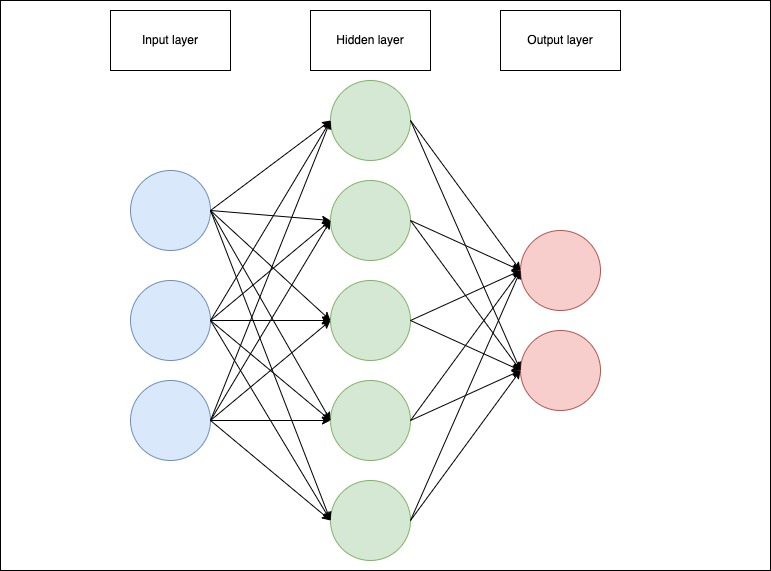
\includegraphics[width=\linewidth]{Figures/Machinelearning/nn_diagram.jpeg}
    \caption[Simple diagram of a neural network]{Simple neural network diagram drawm using Draw.io. Here the blue dots are the input layer, the green dots are a hidden layer, 
    and the red dots are the output layer. The arrows shows the connections between the nodes. }
    \label{fig:nndiagram}
\end{figure}

In order to avoid confusion, we will adhere to table \ref{tab:notation} for the notation used in the following sections.
Some of the following subsections contains work previously done by myself and two co-students, and can be found here\cite{FYSSTK}.

% Define new columns types 
\newcolumntype{L}[1]{>{\raggedright\arraybackslash}p{#1}} % left fixed width
\newcolumntype{C}[1]{>{\centering\arraybackslash}p{#1}} % center fixed width
\newcolumntype{R}[1]{>{\raggedleft\arraybackslash}p{#1}} % flush right fixed width
\begin{table}[H]
    % \setlength{\tabcolsep}{15pt}
    \renewcommand{\arraystretch}{1.3}
    \begin{center}
    \begin{tabular}{|C{1.5cm}|L{4cm}|C{2cm}|} \hline
    \multicolumn{3}{|c|}{Matrices and vectors}  \\ \hline
    Notation & \multicolumn{1}{c|}{Description} & Type \\ \hline
    $X$ & Design Matrix (input data). & $\mathbb{R}^{N\times \text{\#features}}$ \\ \hline
    $t$ & Target values. & $\mathbb{R}^{N\times \text{\#categories}}$ \\ \hline
    $y$ & Model output, the prediction from our network. &  $\mathbb{R}^{N\times \text{\#categories}}$\\ \hline
    $W^l$ & The weight matrix associated with layer $l$ which handles the connections between layer $l-1$ and $l$ . & $\mathbb{R}^{n_{l-1} \times n_l}$ \\ \hline
     $B^l$ & The bias vector associated with layer $l$ which handles the biases for all nodes in layer $l$.  & $\mathbb{R}^{n_{l} \times 1}$ \\ \hline
   
    \multicolumn{3}{|c|}{Elements}  \\ \hline
    $w^l_{ij}$ & The weight connecting node $i$ in layer $l-1$ to node $j$ in layer $l$. & $\mathbb{R}$ \\ \hline
    $b^l_j$ & Bias acting on node $j$ in layer $l$.  & $\mathbb{R}$ \\ \hline
    $z^l_j$ & Node output before activation on node $j$ on layer $l$. & $\mathbb{R}$\\ \hline
    $a^l_j$ & Activated node output on node $j$ on layer $l$. & $\mathbb{R}$ \\ \hline
    \multicolumn{3}{|c|}{Functions}  \\ \hline
    $C$ & \multicolumn{2}{l|}{Cost function} \\ \hline
    $\sigma^l$ & \multicolumn{2}{l|}{Activation function associated with layer $l$.} \\ \hline
    \multicolumn{3}{|c|}{Quantities }  \\ \hline
    $n_l$ & \multicolumn{2}{l|}{The number of nodes in layer $l$.} \\ \hline
    $L$ & \multicolumn{2}{l|}{Number of layers in total with $L-2$ hidden layers.} \\ \hline
    $N$ & \multicolumn{2}{l|}{Total number of data points.} \\ \hline
    \multicolumn{3}{|l|}{All indexing starts from 1: $i,j,k,l = 1, 2, \hdots$}  \\ \hline
    \end{tabular}
    \caption[Neural network notation]{Table containing notation used for deriving the mathematical formulas for the neural 
    network fetched from previous work\cite{FYSSTK}. }
    \label{tab:notation}
\end{center}
\end{table}
   

\subsection*{Gradient descent}
Let us now consider a general n-dimensional problem, with parameters $\boldsymbol{\theta} = \{\theta_1, \theta_2, ..., \theta_n\}$. 
Our objective is to find the set of $\boldsymbol{\theta}$ to minimize a cost function with respect to the data and target. 
One way to solve this problem is using ordinary least squares. For this approach, 
the optimal paramters $\boldsymbol{\theta_{opt}}$ are derived from minimizing the cost function, as shown here:
\begin{equation*}
    \boldsymbol{\theta_{opt}} = (\boldsymbol{X}^T\boldsymbol{X})^{-1}\boldsymbol{X}^T\boldsymbol{t},
\end{equation*}
where $\boldsymbol{X}$ is the design matrix containing the data, and $\boldsymbol{t}$ is the target vector. This however leads to a problem. Suppose the design matrix is sufficiently large,
then the matrix inversion will get computaitonally expensive, or it might not even exist for a given $\boldsymbol{X}$. Thus, an alternative approch is to iteratively approximate the ideal 
parameters. \par 
Suppose we we have a cost function $C(\boldsymbol{\theta})$ for a given problem. We can approximate the minimum of the cost function by calculating
the gradient $\nabla_{\theta}C$ with respect to $\boldsymbol{\theta}$. The negative of this gradient indicates the direction for the minimum of $C$ when evaluating 
it in a specific point $\boldsymbol{\theta}_i$ in the parameter space \cite{FYSSTK}. This is formulized as follows 
\begin{equation}
    \boldsymbol{\theta}_{i+1} = \boldsymbol{\theta}_i - \eta\nabla_{\theta}C(\boldsymbol{\theta}_i),
\end{equation}
where $\eta$ is a step size, also called the learning rate. The choice of $\eta$ is not a trivial case. It is one of several 
hyperparameters\cite{Goodfellow-et-al-2016} that can be altered, and that highly depend on the given problem. 
With regards to the learning rate, there are only three situations to consider, shown in figure \ref{fig:lr_choice}.

\begin{figure}[H]
    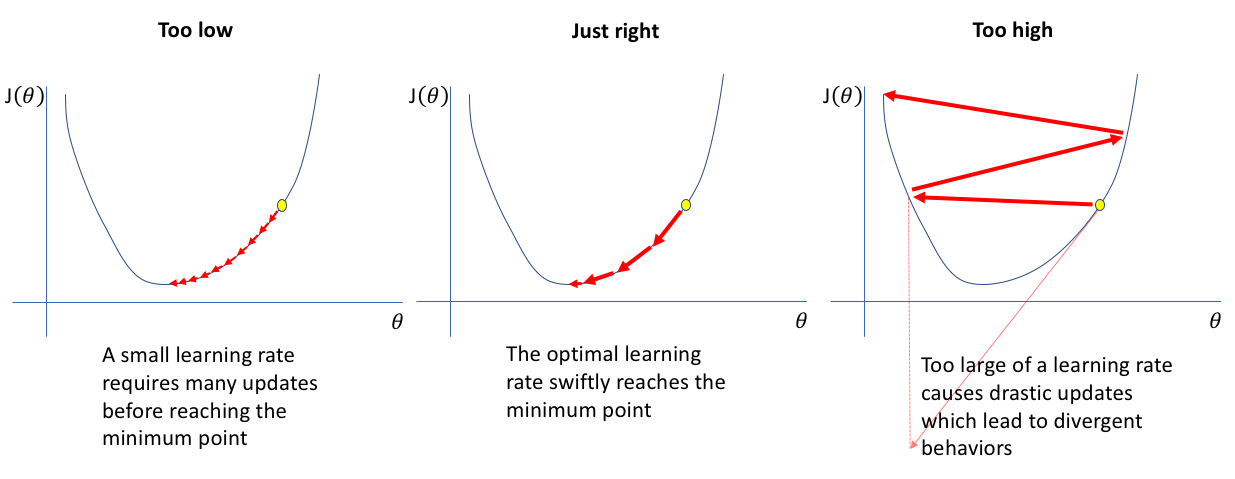
\includegraphics[width=\linewidth]{Figures/Machinelearning/lr_choice.png}
    \caption[Explaining concequence of choice of learning rate]{Figures showing different choices of learning rate for a given cost function, with respect to the tunable parameters. 
    Source: \href{https://www.jeremyjordan.me/content/images/2018/02/Screen-Shot-2018-02-24-at-11.47.09-AM.png}{Jeremy Jordan}, accessed 03.10.22.}
    \label{fig:lr_choice}
\end{figure}

Figure \ref{fig:lr_choice} visualizes the relation between the learning rate and the cost function. 
In the left most figure we note that the learning rate is too small. This leads to many iterations 
before you reach a minimum. In the right most figure we note that the learning rate is too high, 
and the result is that we get divergent behavior. Thus the goal is to find the optimal learning 
rate, shown in the middle figure. There are several algorithms that tries to do what is shown in 
the middle figure above, of of which is ADAM\cite{ADAM:opti}\par 
A modified and prefered version of gradient descent is the so called stochastic gradient descent.
Regular gradient descent can, for large datasets be quite slow, and is prone to getting stuck 
in a local minima. To circumvent this issue, mini batches are introduced. 




\subsection*{Feed forwarding}
Inference (prediction) and training both use the same feed-forward algorithm. Lets then assume that we have generated a 
network. The network initializes the weights and biases usually with normal or uniformly distributed values, that can 
later be adjusted. The procedure is to send the data through the network, weighting each connection according to the networks 
architecture, and produce an output. The procedure can be summarized in the following steps\cite{FYSSTK}:
 \begin{itemize}
    \item The data is recieved by the input nodes in the network for each feature.
    \item Each input node weights the data value according to the connection of each node in the next layer.
    \item Every node in the hidden layers sums the weighted data values and adds the bias associated to the given node. The resulting number is denoted as z. 
    \item This value z is then sent through an activation function $\sigma$, which produces the output of the node, denoted as $a = \sigma(z)$.
    \item This process is repeated for each hidden layer, and it is important to note that the number of nodes in the hidden layers is not dependent on the number of features in the original dataset. 
    \item The last hidden layer then sends the activated values to the output layer, where the number of nodes and choice of activation function depends on the problem to solve.
 \end{itemize}

Mathematically this is expressed as follows:
\begin{equation}
    z_j^l = \sum_{i=1}^{n_{l-1}} w_{ij}^l a_i^{l-1} + b_j^l, \quad a_j^l = \sigma^l(z_j^l),
\end{equation}
where $l$ is the layer index, $j$ is the node index, and $i$ is the index of the node in the previous layer, 
and $l \neq 1$, as it is not used on the input layer.


\subsection*{Backpropagation}
The way neural networks learn is conventionally by the use of the backpropagation algorithm, first proposed by 
Rumelhart et al\cite{backprop}. This is a bit misleading, as the backpropagation algorithm actually only refers 
to how to compute the gradient\cite{Goodfellow-et-al-2016}. The algorithm allows us to alter the weights and 
biases such thatwe get an ideal output. Assuming a cost function $C$, we can calculate the gradient $\nabla_{w, b}C$,
and use this to back propagate the error correction. The gradient $\nabla_{w, b}C$ is comprised of two derivatives.
 

\begin{equation*}
    \nabla_{w, b}C = \left(\frac{\partial C}{\partial w_{i,j}^l}, \frac{\partial C}{\partial b_j^l}\right).
\end{equation*}

We have to use the chain rule to calculate the derivatives, and using that the last layer is $l=L$, we get the derivative with respect to the weights as 

\begin{equation*}
    \frac{\partial C}{\partial w_{i,j}^L} = \frac{\partial C}{\partial a_j^L}\frac{\partial a_j^L}{\partial z_j^L}\frac{\partial z_j^L}{\partial w_{i,j}^L},
\end{equation*}
where 
\begin{equation*}
    a_j^L = \sigma(z_j^L), \quad z_j^L = \sum_{i=1}^{n_L-1} w_{i,j}^La_i^{L-1} + b_j^L.
\end{equation*}

This then gives us 
\begin{equation*}
    \frac{\partial C}{\partial w_{i,j}^L} = \frac{\partial C}{\partial a_j^L}\sigma'(z_j^L)a_i^{L-1},
\end{equation*}
where we defined that 
\begin{equation}\label{eq:sigma_der}
    \sigma'(z_j^L) = \frac{\partial a_j^L}{\partial z_j^L}.
\end{equation}

This derivative is very easy to calculate given a specific cost function and activation function. The derivative with respect to the bias is given as follows:

\begin{equation*}
    \frac{\partial C}{\partial b_k^L} = \frac{\partial C}{\partial a_j^L}\frac{\partial a_j^L}{\partial z_j^L}\frac{\partial z_j^L}{\partial b_{j}^L},
\end{equation*}
which gives us the final expression as 

\begin{equation*}
    \frac{\partial C}{\partial b_k^L} = \frac{\partial C}{\partial a_j^L}\sigma'(z_j^L). 
\end{equation*}

We will now introduce a new notation, a local gradient commonly called the "error". It reflects how the rate of change of the cost function depends on the j'th node in the l'th layer.

\begin{equation*}
    \delta_j^l \equiv \frac{\partial C}{\partial z_j^l}.  
\end{equation*}
Using this we get the following expression:

\begin{equation*}
    \delta_j^L=  \frac{\partial C}{\partial z_j^L} = \frac{\partial C}{\partial a_j^L}\frac{\partial a_j^L}{\partial z_j^L} = \frac{\partial C}{\partial a_j^L}\sigma'(z_j^L),
\end{equation*}

giving us the more compact forms of the derivatives with respect to the weights and biases:

\begin{equation*}
    \frac{\partial C}{\partial w_{i,j}^L} = \delta_j^La_i^{L-1}, \quad \frac{\partial C}{\partial b_j^L} = \delta_j^L.
\end{equation*}

We can now let $\boldsymbol{\delta^l}$ be the vector of all the errors in the l'th layer, and $\boldsymbol{\delta^L}$ be the vector of all the errors in the last layer. 
The error in the l'th layer can then be expressed as a matrix equation for the last layer as follows:

\begin{equation*}
    \boldsymbol{\delta^l} = \nabla_aC \odot \frac{\partial \sigma}{\partial z^L}, \quad \nabla_aC = \left[\frac{\partial C}{\partial a_1^L}, \frac{\partial C}{\partial a_2^L}, ..., \frac{\partial C}{\partial a_{n_L}^L} \right]^T.
\end{equation*}

Here $\odot$ is the Hadamard product (element wise product). This local gradient can now be defined recursively for the j'th node in a layer l as a function of the local error in the next layer:

\begin{equation}
    \label{eq:localgradient}
    \delta_j^l \equiv \frac{\partial C}{\partial z_j^l} = \sum_k \frac{\partial C}{\partial z_k^{l+1}}\frac{\partial z_k^{l+1}}{\partial z_j^l} = \sum_k \frac{\partial z_k^{l+1}}{\partial z_j^l} \delta_k^{l+1}.
\end{equation}

We also note that 
\begin{equation*}
    z_k^{l+1} = \sum_{j=1}^{n_l} w_{j,k}^{l+1}a_j^l + b_k^{l+1} = \sum_{j=1}^{n_l} w_{j,k}^{l+1}\sigma(z_j^l) + b_k^{l+1},
\end{equation*} 
thus the partial derivative is given as 

\begin{equation}
    \label{eq:dzl1dz}
    \frac{\partial z_k^{l+1}}{\partial z_j^l} = w_{j,k}^{l+1}\sigma'(z_j^l), 
\end{equation}
using the substitution from equation \ref{eq:sigma_der}. This allows us to substitute equation \ref{eq:dzl1dz} into equation \ref{eq:localgradient} to get the following expression:

\begin{equation}
    \label{eq:localgradient2}
    \delta_j^l = \sum_k w_{j,k}^{l+1}\sigma'(z_j^l)\delta_k^{l+1}.
\end{equation}

Using this we can derive a three step formula for the backpropagation algorithm:
\begin{itemize}
    \item Compute the local gradient for the last layer, $\delta^L$.
    \item Recursively compute the local gradient for the remaining layers, $\delta^l$ for $l=L-1, L-2, ..., 1$.
    \item Update the weights and biases for all layers, $l=1, 2, ..., L$, given the learning rate $\eta$ as shown below: 
\end{itemize}

\begin{equation*}
    w_{i,j}^{l} \leftarrow w_{i,j}^{l} - \eta \delta_j^l a_i^{l-1},
\end{equation*}


\begin{equation*}
    b_j^l \leftarrow b_j^l - \eta \delta_j^l.
\end{equation*}

\section*{Autoencoders}
Autoencoders are a subset of neural networks. Whereas a general neural network
 in principle can take any shape, autoencoders are more restrictive.
This restrictiveness can in its most general sence we condensed 
into the following points:
\begin{itemize}
    \item Same number of output categories as input categories  
    \item A latent space with smaller dimensionality than the input/output layer  
\end{itemize}
What we end up with two funnel shaped parts linked together. The two funnels are 
called the encoder (left funnel) and decoder (right funnel) respectively. This architecture is not 
accidental, but rather designed with a very specific solution of ploblems in mind, reconstruction. 
A good example to illustrate this is image denoising. Suppose you have a noised image, 
and want to denoise it. By feeding the encoder a noised image, and comparing the decoder output 
to the actual image, the autoencoder can tune itself to denoise images. 
\section{Other tools and algorithms}
\subsection*{Adaptable moment estimation (ADAM) Optimizer}
Stochastic gradient descent, though very useful, lack the ability to adapt to the feature space. One algorithm that address this
issue is the ADAM optimizer\cite{ADAM:opti}. The Adaptable moment estimation (ADAM) algorithm uses stochastic gradient descent, but with 
an adaptiv learning rate. This learning rate is adjusted by calculating estimates for the first and second moment\footnote{In statistics
the first moment is the expectation value for a distribution, $E[X-\mu]$. The second moment is the 
expectation value of the distribution squared, i.e the variance, $E[(X-\mu)^2]$}. Thus, a large gradient would indicate close proximity 
to a minimum in feature space, thus a lower learning rate would yield a more accurate result, 
where as a small gradient would suggest far proximity to a local minimum, and thus a larger learning rate would increase the chance 
of approaching a minimum.\par 

\subsection*{Hyperband}
Hyperband is a tool for hyperparameter optimization\cite{hyperband:opt}. Hyperparameter optimization is of high importance in the 
search for ideal structures and architectures when using neural networks, as there is not a way to find an a priori setup for a 
given problem. Several algorithms are used, from random search, grid search, and bayesian optimization. Hyperband is an algorithm 
proposed by L. Li et al. It focuses on using successful halving\cite{successivehalving}
but at the same time doing a grid search for how to allocate resources. Successive halving focuses on testing n configurations, and removing 
the bottom half, thus (hopefully) quickly converging to the ideal combination. However, it is not easy to a priori know the 
number of configurations n, and how much resources one needs, r, to quickly find the ideal set. This is where Hyperband comes in. 
In essence, it fetches and tries different combinations of r resources (time, data set subsampling or feature subsampling) and n 
configurations, to determine the ideal set of hyperparameters via successive halving, yielding 5x to 30x speedup compared to 
Bayesian optimization. One drawback for this algorithm is that one cannot guarantiy that the configuration is optimal, 
but rather that it is good enough. 

\subsection*{Activation functions}
Several activation functions are used in neural networks, and how one chooses the best combination for a given problem is not trivial. 
This leads often to the use of tuning. Below are a list of the functions used in this thesis, aswell as their mathematical definitions. 

\begin{enumerate}
    \item  $sigmoid(x) = \frac{1}{1+e^{-x}}$
    \item $tanh(x) = \frac{e^x-e^{-x}}{e^x+e^{-x}}$
    \item $ReLU(x) = \max(0,x)$
    \item $LeakyReLU(x) = \max(\alpha x,x)$
    \item $Softmax(x) = \frac{e^x}{\sum_{i=1}^n e^x}$
    \item $Linear(x) = x$
\end{enumerate}


\subsection*{ROC curve}
One way to measure the effectiveness of a prediction for a machine learning algorithm is with the use of a ROC curve. 
The ROC curve is a plot of the true positive rate (TPR) against the false positive rate (FPR) which will be defined shortly. 
Suppose a classifier $\mathcal{M}$ does a binary classification of positive and negative. If $\mathcal{M}$ predicts a positive 
label, and the instance is indeed positive, we define this as a $\it{true\, positive}$. The same goes for negative prediction of a 
negative instance, which is defined as a $\it{true\, negative}$. Then there is the case where $\mathcal{M}$ predicts a negative label
when the instance is positive, defined as a $\it{false\, negative}$, and vice versa is then defined as a $\it{false\, positive}$\cite{FAWCETT2006861}.
Now, the TPR is defined as the ratio of true positives to the total number of positive instances, i.e 
\begin{equation*}
    TPR = \frac{TP}{TP+FN},
\end{equation*}
and the FPR is defined as the ratio of false positives to the total number of negative instances, i.e
\begin{equation*}
    FPR = \frac{FP}{FP+TN}.
\end{equation*}
Using this, we get a plot that tells us how well the classifier performs. As the goal usually is it to have a high TPR and a low FPR,
the more "north west"\cite{FAWCETT2006861} of the plot the curve is, the better. Below are two example of a ROC curve and the classifier output it 
is calculated from. For simplicity, the classifier output is in this case just two normal distributions with the mean and standard deviation 
listed in the legend of the distribution plots.

\begin{figure}[H]
    \centering
    \begin{subfigure}{.45\textwidth}
        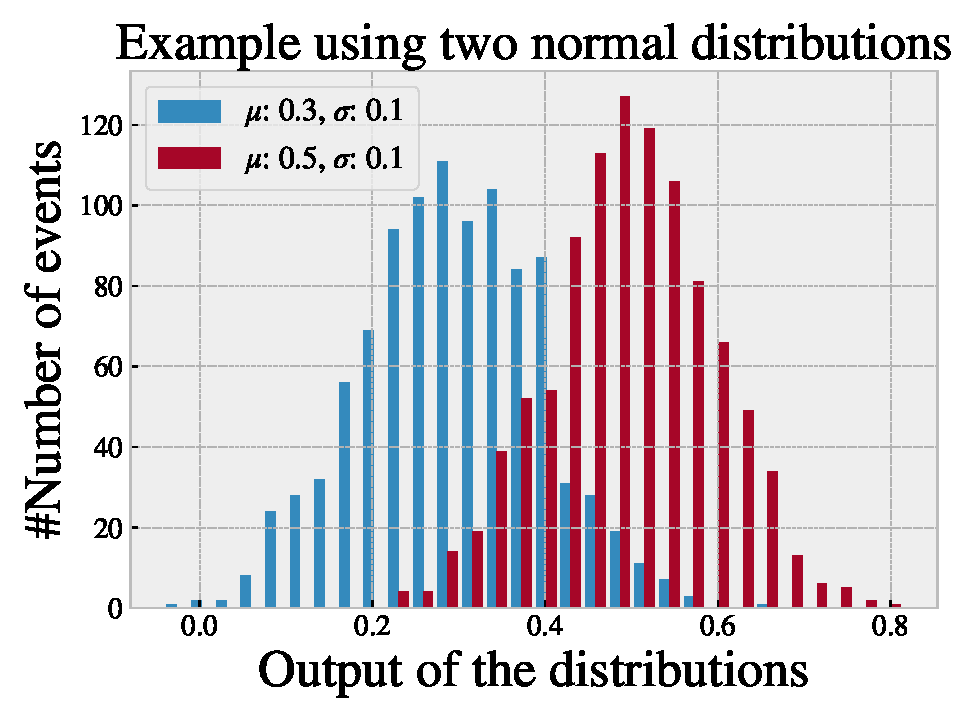
\includegraphics[width=\textwidth]{Figures/Machinelearning/histo_example_Sep.pdf}
        \caption{Histogram showing good separation. Here the left distribution is calculated using a mean of 0.3 and a standard 
        deviation of 0.1, and the right distribution is calculated using a mean of 0.5 and a standard deviation of 0.1.}
        \label{fig:dist_ex_good}
    \end{subfigure}
    \hfill
    \begin{subfigure}{.45\textwidth}
        \includegraphics[width=\textwidth]{Figures/Machinelearning/ROC_curve_example_Sep.pdf}
        \caption{ROC curve based on the two distributions to the left. Here we get an area under the curve score of 0.92, which is very good. }
        \label{fig:ROC_curve_ex_good}
    \end{subfigure}
    \hfill        
    \caption{Histogram and ROC curve for two well separated distributions.}
    \label{fig:roc_example_good}
\end{figure}

\begin{figure}[H]
    \centering
    \begin{subfigure}{.45\textwidth}
        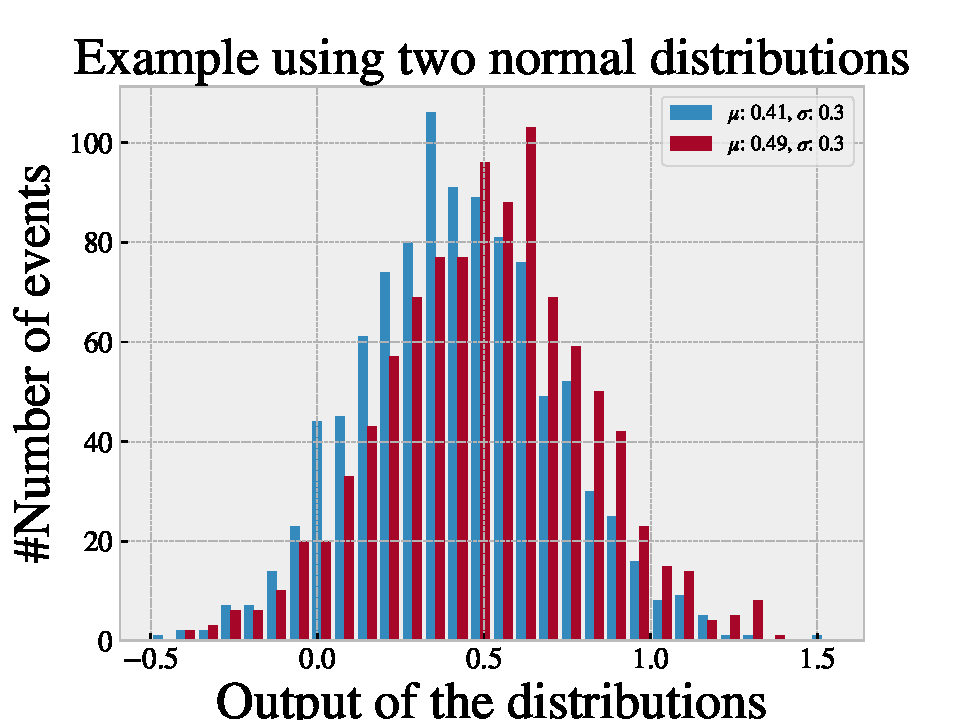
\includegraphics[width=\textwidth]{Figures/Machinelearning/histo_example_bad.pdf}
        \caption{Histogram showing bad separation. Here the left distribution is calculated using a mean of 0.41 and a standard 
        deviation of 0.3, and the right distribution is calculated using a mean of 0.49 and a standard deviation of 0.3.}
        \label{fig:dist_ex_bad}
    \end{subfigure}
    \hfill
    \begin{subfigure}{.45\textwidth}
        \includegraphics[width=\textwidth]{Figures/Machinelearning/ROC_curve_example_bad.pdf}
        \caption{ROC curve based on the two distributions to the left. Here we get an area under the curve score of 0.58, which is not a good classification score.}
        \label{fig:ROC_curve_ex_bad}
    \end{subfigure}
    \hfill        
    \caption{Histogram and ROC curve for two poorly separated distributions.}
    \label{fig:roc_example_bad}
\end{figure}

In figure \ref{fig:roc_example_good} we have a histogram showing two distributions that are well separated, and the ROC curve that is calculated 
based on thos distributions. If we compare this to figure \ref{fig:roc_example_bad}, we see that the better separation of the two distributions, the better ROC curve. 
This is a useful tool to use with the autoencoder, as it provides valueable insight beyond just looking at the output distributions.

\subsection*{Statistical significance}
In the frequentist statistics, the Poisson distribution can be approximated with a Gaussian distribution in the limit of large number of events\cite{magnar}. 
The expression for the significance is given then as 
\begin{equation}\label{eq:significance_large}
    Z = \frac{s}{\sqrt{b}},
\end{equation}
where s is the amount of signal, and b is the amount of background. For low statistics we have that the significance is given as 
\begin{equation}\label{eq:significance_small}
    Z = \sqrt{2\left[(s+b)\ln(1+\frac{s}{b})-s\right]}.
\end{equation}
It can be shown that in the limit where $s << b$, the two expressions are approimately the same\cite{magnar}.

%%%%%%%%%%%%%%  SM and BSM  %%%%%%%%%%%%%%%%%%%%%%%
\chapter{The Standard model and BSM physics}\label{Chap:SM}

\begin{figure}[h!]
    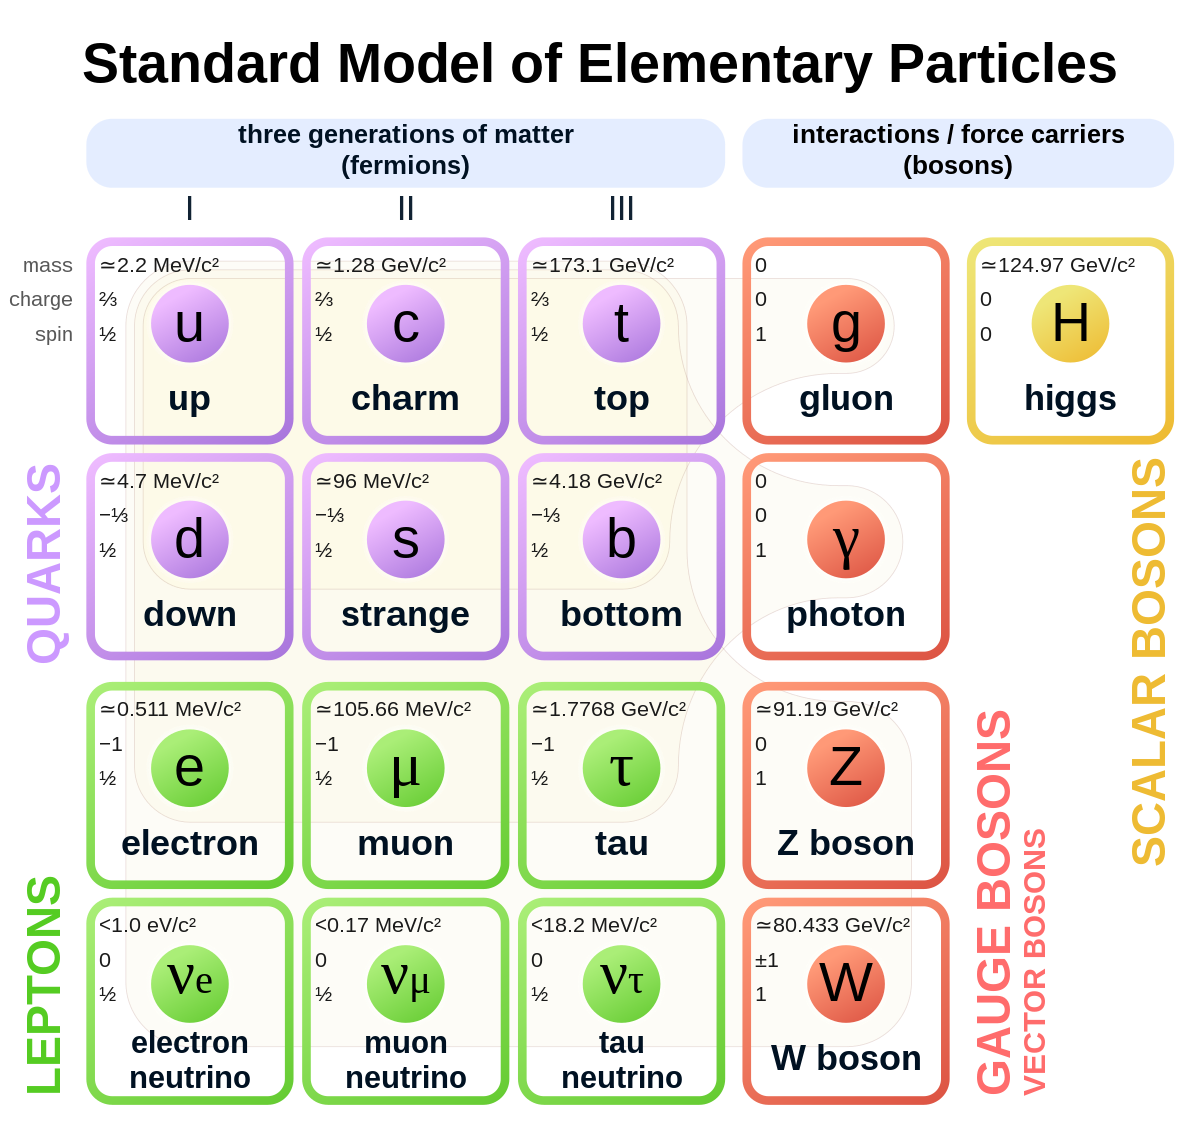
\includegraphics[width=\linewidth]{Figures/SM/Standard_Model_of_Elementary_Particles.svg.png}
    \caption{The standard model of elementary particles. Source \href{https://upload.wikimedia.org/wikipedia/commons/thumb/0/00/Standard_Model_of_Elementary_Particles.svg/1200px-Standard_Model_of_Elementary_Particles.svg.png}{here}. Accessed 07.10.22}
    \label{fig:smdiagram}
\end{figure}

\section{Structure and composition of the Standard Model}
This section will describe the standard model in a phenomelogical way, as the mathematics and physical reasoning behind the theory is not of great 
importance to understand the work, nor the results or discussion of them. For a more technical explanation, read (Pich, 2008)\cite{Pich:819632} for a 
well written paper containing the some more standard model fundamentals, as well as summarizing the experimental status regarding the standard model.
For more mathematical understanding of the standard model, Peskin and Schroeder's "An introduction to Quantum Field theory" (Peskin and Schroeder, 1995)\cite{Peskin:1995ev}
 is highly recommended. Finally, see Thomson's "Modern Particle physics" (Thomson, 2013)\cite{Thomson:2013zua} for a very comprehensive and up-to-date book that is easy to read and understand. \par
The standard model is to physicists what the periodic table is to chemists, and is to this day the most fundamental description of matter as we know it. 
It is comprised of two parent class particles, fermions and bosons, where fermions are comprised of quarks and leptons. The model contains 
17 particles, 6 quarks, 6 leptons and 5 bosons, and are shown in figure \ref{fig:smdiagram}.



\subsection*{Fermions}
The fermions are the building blocks of matter, and contain two types of particles, leptons and quarks. Together they form protons and neutrons,  atoms all around us.
Fermions, unlike bosons, are spin half particles, and are also the only particles to have anti particles. The fermions are grouped into three so called families:
\begin{equation*}
    \begin{bmatrix}
        \nu_e & u \\
        e^{-} & d^{\, '} 
    \end{bmatrix},\quad
    \begin{bmatrix}
        \nu_{\mu} & c \\
        \mu^{-} & s^{\, '}
    \end{bmatrix},\quad
    \begin{bmatrix}
        \nu_{\tau} & t \\
        \tau^{-} & b^{\, '}
    \end{bmatrix}
\end{equation*}
Note that the left column contains the leptons. whilst the right column contains the quarks. Within the left column, the subscripted $\nu$ denotes what kind of neutrino that corresponds 
to the given lepton. Here, the first family consists of the electron, the electron neutrino, the up and down quarks. The second family consists of the muon and the
muon neutrino, the charm and strange quarks. The third family consists of the tau and the tau neutrino, the top and bottom quarks. The masses of these particles 
increases for each particle in the matrix as the family number increases, i.e the muon is heavier than the electron, and the tau is heavier than the muon, and so 
on for the other fermions. Below is a table with specific properties of the fermions.\par

% Please add the following required packages to your document preamble:
% \usepackage{multirow}
\begin{table}[h!]
    \caption{Table showing properties of all the fermions, including name, symbol, antiparticle, spin, charge, generation and mass.}
    \label{tab:fermion_table}
    \begin{tabular}{|ccccccc|}
    \hline
    \multicolumn{1}{|l|}{\textbf{Generation}}         & \multicolumn{1}{l|}{\textbf{Name}}     & \multicolumn{1}{l|}{\textbf{Symbol}} & \multicolumn{1}{l|}{\textbf{Antiparticle}} & \multicolumn{1}{l|}{\textbf{Spin}} & \multicolumn{1}{l|}{\textbf{Charge}} & \multicolumn{1}{l|}{\textbf{Mass (MeV$/c^2$)}} \\ \hline
    \multicolumn{7}{|c|}{\textbf{Quarks}}                                                                                                                                                                                                                                                                       \\ \hline
    \multicolumn{1}{|c|}{\multirow{2}{*}{\textbf{1}}}                  & \multicolumn{1}{c|}{up}                & \multicolumn{1}{c|}{u}               & \multicolumn{1}{c|}{$\bar{u}$}             & \multicolumn{1}{c|}{$1/2$} & \multicolumn{1}{c|}{$2/3$}   & $2.2_{-0.4}^{+0.6}$                            \\ \cline{2-7} 
    \multicolumn{1}{|c|}{}                   & \multicolumn{1}{c|}{down}              & \multicolumn{1}{c|}{d}               & \multicolumn{1}{c|}{$\bar{d}$}             & \multicolumn{1}{c|}{$1/2$} & \multicolumn{1}{c|}{$-1/3$}  & $4.6_{-0.4}^{+0.5}$                            \\ \hline
    \multicolumn{1}{|c|}{\multirow{2}{*}{\textbf{2}}} & \multicolumn{1}{c|}{charm}             & \multicolumn{1}{c|}{c}               & \multicolumn{1}{c|}{$\bar{c}$}             & \multicolumn{1}{c|}{$1/2$} & \multicolumn{1}{c|}{$2/3$}   & $1280 \pm 30$                                  \\ \cline{2-7} 
    \multicolumn{1}{|c|}{}                            & \multicolumn{1}{c|}{strange}           & \multicolumn{1}{c|}{s}               & \multicolumn{1}{c|}{$\bar{s}$}             & \multicolumn{1}{c|}{$1/2$} & \multicolumn{1}{c|}{$-1/3$}  & $96_{-4}^{+8}$                                 \\ \hline
    \multicolumn{1}{|c|}{\multirow{2}{*}{\textbf{3}}} & \multicolumn{1}{c|}{top}               & \multicolumn{1}{c|}{t}               & \multicolumn{1}{c|}{$\bar{t}$}             & \multicolumn{1}{c|}{$1/2$} & \multicolumn{1}{c|}{$2/3$}   & $172100 \pm 600$                               \\ \cline{2-7} 
    \multicolumn{1}{|c|}{}                            & \multicolumn{1}{c|}{bottom}            & \multicolumn{1}{c|}{b}               & \multicolumn{1}{c|}{$\bar{b}$}             & \multicolumn{1}{c|}{$1/2$} & \multicolumn{1}{c|}{$-1/3$}  & $4180_{-30}^{+40}$                             \\ \hline
    \multicolumn{7}{|c|}{\textbf{Leptons}}                                                                                                                                                                                                                                                                               \\ \hline
    \multicolumn{1}{|c|}{\multirow{2}{*}{\textbf{1}}}                & \multicolumn{1}{c|}{electron}          & \multicolumn{1}{c|}{$e^-$}           & \multicolumn{1}{c|}{$\bar{e}^-$}           & \multicolumn{1}{c|}{$1/2$} & \multicolumn{1}{c|}{-1}              & $0.511$                                        \\ \cline{2-7} 
    \multicolumn{1}{|c|}{}                   & \multicolumn{1}{c|}{electron neutrino} & \multicolumn{1}{c|}{$\nu_{e}$}       & \multicolumn{1}{c|}{$\bar{\nu}_e$}         & \multicolumn{1}{c|}{$1/2$} & \multicolumn{1}{c|}{0}               & $<0.0000022$                                   \\ \hline
    \multicolumn{1}{|c|}{\multirow{2}{*}{\textbf{2}}} & \multicolumn{1}{c|}{muon}              & \multicolumn{1}{c|}{$\mu^-$}         & \multicolumn{1}{c|}{$\bar{\mu}^-$}         & \multicolumn{1}{c|}{$1/2$} & \multicolumn{1}{c|}{-1}              & $105.7$                                        \\ \cline{2-7} 
    \multicolumn{1}{|c|}{}                            & \multicolumn{1}{c|}{muon neutrino}     & \multicolumn{1}{c|}{$\nu_{\mu}$}     & \multicolumn{1}{c|}{$\bar{\nu}_{\mu}$}     & \multicolumn{1}{c|}{$1/2$} & \multicolumn{1}{c|}{0}               & $<0.170$                                       \\ \hline
    \multicolumn{1}{|c|}{\multirow{2}{*}{\textbf{3}}} & \multicolumn{1}{c|}{tau}               & \multicolumn{1}{c|}{$\tau$}          & \multicolumn{1}{c|}{$\bar{\tau}$}          & \multicolumn{1}{c|}{$1/2$} & \multicolumn{1}{c|}{-1}              & $1776.86 \pm 0.12$                             \\ \cline{2-7} 
    \multicolumn{1}{|c|}{}                            & \multicolumn{1}{c|}{tau neutrino}      & \multicolumn{1}{c|}{$\nu_{\tau}$}    & \multicolumn{1}{c|}{$\bar{\tau}_{\tau}$}   & \multicolumn{1}{c|}{$1/2$} & \multicolumn{1}{c|}{0}               & $< 15.5$                                       \\ \hline
    \end{tabular}
    \end{table}

Quarks are fractional charge particles, with defined charge of either $2/3$ or $-1/3$, as shown in table \ref{tab:fermion_table}. They are the "main" building blocks of protons and neutrons, and are bound by the strong 
force, the strongest of the four fundamental forces. The force mediator is the gluon. The other half of fermions are the leptons. They are split into the charged 
leptons (electrons, muons and taus), and the uncharged leptons (neutrinos). The charged leptons can interact via the electroweak force, where the Z, W bosons 
as well as the photon can be a mediator.


\subsection*{Bosons}
Bosons are integer number spin particles, with spin $0, 1, 2, ...$. Within bosons there are so called elementary bosons, some of which are force carriers or mediators such as the W, Z and the photon.
The Higgs boson is also an elementary boson, but is not a force carrier. It provides masses for the fermions via a process called spontaneous symmetry breaking\cite{Pich:819632}. Other 
bosons are so called composite bosons, which are particles constructed by an even amount of fermions yeilding the integer spin. 

\subsection*{Left and right handedness}
Particles in the standard model are subject to a quantum mechanical property called chirality. 
Chirality is a property that describes a particle's ability to be superimposed on its mirror image. 
If a particle has chirality, it cannot be superimposed on its mirror image by any combination of translation, 
rotation, and reflection operations. \cite{weinberg_1995}

\subsection*{Feynman diagrams}
A graphical way to understand particle interactions are through so called Feynman diagrams. Feynman diagrams are drawn based on the Feynman rules for a given Lagrangian\cite{Pich:819632}\cite{feynrules}, and each component 
can be linked to a part in the Lagrangian for the system. 

\begin{figure}[h!]
    \centering
    \caption{Feynman diagram of muon pair production from electron scattering. Here, both Z and $\gamma$ can work as the propagator.}
    
\begin{tikzpicture}
    \begin{feynman}
    
        \vertex at (0.5, 1.) (a2){\(e^{-}\)} ;
        \vertex at (0.5, -1.)  (a5){\(e^{+}\)} ;

        \vertex at (1.5, 0.0) (c);
        \vertex at (3., 0.0) (d);

        \vertex at (4, 1.) (f1) {\(\mu^{-}\)} ;
        \vertex at (4,-1.) (f2) {\(\mu^{+}\)};

        
    \diagram*{


        (a2) -- [fermion] (c) -- [boson] (d),
    
        (a5) -- [anti fermion] (c) -- [boson, edge label = {$\gamma, Z$}] (d),
        (d) -- [fermion] (f1),
        (d) -- [anti fermion] (f2),
        
        ;
    };
    \end{feynman}
    \end{tikzpicture}
    \label{fig:eemm_scat}
\end{figure}

In figure \ref{fig:eemm_scat} we have a Feynman diagram describing two scenarios: electron scattering into muon pairs and 
electron muon scattering into electron muon. This is because we have not yet set the direction for time evolution. In this thesis, all 
diagrams will be interpreted from left to right, i.e figure \ref{fig:eemm_scat} then only represents electron scattering into muon pair. 
The diagram contains all the components in the Lagrangian, and arrows, curly lines and so on all have its own meaning. A straight line with 
an arrow usually means a fermion, where the direction of the arrow tells if the particle (arrow towards the vertex) is an anti particle (arrow away from the vertex) 
or particle, showing the momentum direction essentially. The is often also a propagator between the input and the output of such processes, 
and they depend on the processes we want to study. in the diagram above we have lepton scattering, thus we can both have the photon and the 
Z-boson as a propagator. This process is called a neutral current\cite{Pich:819632}, as the total charge coming out of the interaction is 0. 
As with neutral currents, we also have so called charged currents, where the sum of charge is not 0. Note that we only require charge conservation,
thus there is nothing wrong with either having a neutral or a charged current, as long as charge conservation is preserved. \par 
Feynman diagrams is not only used for visualizing scatterings, they can also visualize decays. An example is provided below. 

\begin{figure}[h!]
    \centering
    \caption{Muon decay into an electron, an electron neutrino and a muon neutrino via the $W^{-}$ boson. Read the graph from left to right.}
    
\begin{tikzpicture}
    \begin{feynman}
    
        \vertex at (0.5, 0.) (a2){\(\mu^{-}\)} ;

        \vertex at (2., 0.0) (c);
        \vertex at (3., -1.) (d);
        
        \vertex at (3.5, 0.7) (a3){\(\nu_{\mu}\)} ;

        \vertex at (4, -0.5) (f1){\(e^{-}\)} ;
        \vertex at (4.,-1.4) (f2) {\(\bar{\nu}_{e}\)};

        
    \diagram*{


        (a2) -- [fermion] (c) -- [boson, edge label = {$W^{-}$}] (d),
        (a2) -- [fermion] (c) -- [fermion] (a3),
        (d) -- [fermion] (f1),
        (d) -- [anti fermion] (f2),
        
        ;
    };
    \end{feynman}
    \end{tikzpicture}
    \label{fig:eemm_scat}
\end{figure}

Here we have a decay of a muon into and electron and two neutrinos, through a charged current. 

\subsection*{Some limitations}
All though the standard model have had great success comparing with experiments,
there are still several problems not addressed by it. One example is gravity, the standard model
as described above, does not and cannot explain gravity in a quantized way. There 
are models that try to address this problem, but they supplement the standard model,
and does not derrive it from it. \par 
The problem that will be addressed in this thesis is a curious property of the weak interaction, 
namely that parity is broken. Parity as a mathematical operation is equivalent to the spatial inversion 
through the origin\cite{Thomson:2013zua}:
\begin{equation}
    x \to -x.
\end{equation}
In other words, parity can be thought of as left-right symmetry, or mirror symmetry. Breaking of parity is observed
with weak currents, where the mediator of the charged currents, $W^{\pm}$ only interacts with 
left handed fermions. In the standard model, neutrinos are assumed to be massless, and the righthanded 
neutrinos are sterile, i.e they do not interact with the standard model. \par 
This asymmetry is strange, and hints towards new physics that perhaps can restore the parity breaking. 
Another note to make is that it has been experimentally verified that the neutrinos are massive\cite{Katrin_neutrinos},
with an upper limit on the mass for the anti electron neutrino of $m_{\nu} < 0.8eVc^2$ at $90\%$ confidence level.
This is somewhat problematic, as the masses of the neutrinos are not predicted by the standard model. 









\section{Beyond Standard Model (BSM) physics}
The approach of using an autoencoder is an attempt to try and detect BSM physics in an as model agnostic way as possible. This is because there are 
numerous amounts of possible BSM physics signals some of which could exist in nature. To test the autoencoder two 
signals from supersymmetry were used. The testing was performed only after having trained on SM only background.
\subsection*{Supersymmetry}
Supersymmetry is a BSM theory that attempts to solve two problems that the SM has. 
First we have the hierarchy problem. As the SM is a perturbative theory, the Higgs mass increases at 
higher energies. The problem is that when you approach higher and higher energies, the Higgs mass goes to infinity, 
which is not physical. Supersymmetry solves this problem by introducing a supersymmetric partner to each particle
in the SM. The result is that the contributions to the Higgs mass from fermions and bosons mainly cancel each other out, 
thus fixing the hierarchy problem. Another problem we have with the SM
is that is does not have a candidate for dark matter, whereas some supersymmetry models have a dark matter candidate.
As supersymmetry in theory could solve some problems with the SM it is a topic of great interest with both theoretical and 
experimental physicists. Still, after two LHC runs supersymmetry has not been observed\cite{atlas_search_2021}. \par 

To test the autoencoders, two simplified signal models from SUSY were picked up. The chosen signal samples have a final state with 3 leptons + $e_T^{miss}$,
as the background does. The signal final state is shown below in figure \ref{fig:sysy_feyn}. 

\begin{figure}[H]
    \centering
    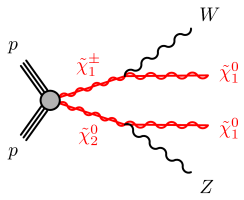
\includegraphics[width=0.4\linewidth]{Figures/susy/C1N2-WZN1N1.png}
    \caption[SUSY feynman diagram]{SUSY diagram showing chargino-neutralino prodiction in proton-proton collision. 
    The test samples we look for with this signal is where the W and Z boson decay leptonically.}
    \label{fig:sysy_feyn}
\end{figure}

Figure \ref{fig:sysy_feyn} shows chargino$(\tilde{\chi}_2^{\pm})$-neutralino$(\tilde{\chi}_1^{0})$ production via proton-proton collisions. 
The charginos are the supersymmetric partners 
to the charged bosons and the neutralinos are the supersymmetric partner of the neutral bosons $(\gamma, Z^0)$ and 
the neutral Higgs bosons $(h, H^0)$\footnote{Supersymmetry spontaneous symmetry breaking leads to 5 physical Higgs bosons: 
$H^0$, $h^0$, $A^0$, $H^{\pm}$}. The neutralino
is the lightest stable supersymmetric particle, and is therefor a good candidate for dark matter. 
The search for these particles was similarly done by ATLAS in 2021\cite{atlas_search_2021}. 

%%%%%%%%%%%%%%  Implementation  %%%%%%%%%%%%%%%%%%%%%%%
\chapter{Implementation}\label{Chap:implementation}

\section{The ATLAS detector}

\subsection*{Kinematics and detector geometry}
Before one can analyse the data, it has to be collected and processed in a detector. The data used in this thesis 
are generated from proton-proton collisions in the ATLAS detector at the LHC. The ATLAS inner detector itself is a solenoid, 
and the kinematic variables are measured based on the following coordinate system. The z-axis is defined to go 
along the center axis of the solenoid, whereas the y-axis points upwards in the detector and the x-axis radialy 
outwards from the center axis. This allows for all transverse variables to be defined in the x-y plane\cite{Gramstad:1631043}. 
From this we contruct the azimuthal and polar angles $\phi$ and $\theta$, where the azimuthal angle $\phi$\cite{Airapetian:391176} is the angle around the z-axis, 
and the polar angle $\theta$ is the angle from the z-axis, as shown in figure \ref{fig:long_trans_plane}.


\begin{figure}[H]
    \centering
    \begin{subfigure}{.45\textwidth}
        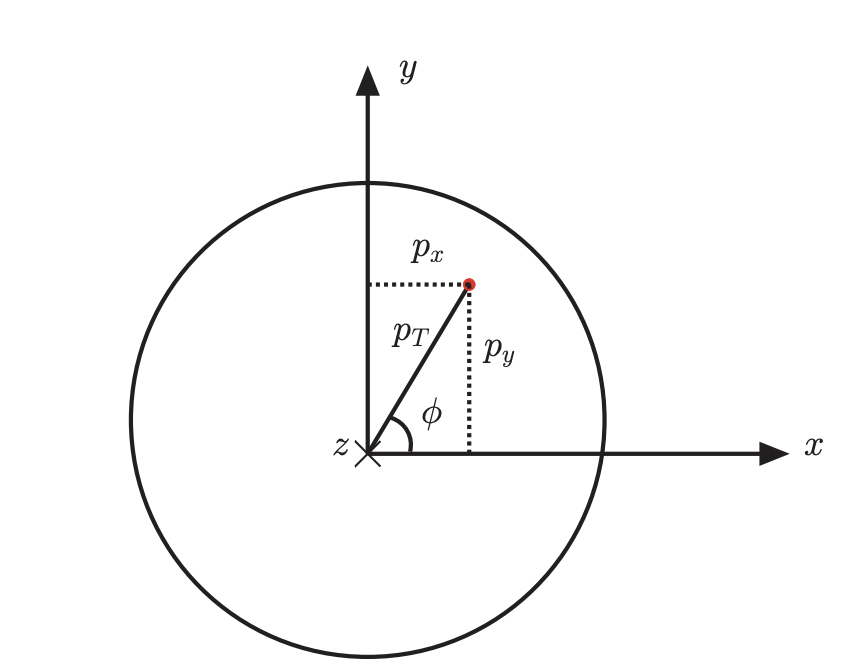
\includegraphics[width=\textwidth]{Figures/atlas/transverse_plane.png}
        \caption{Transverse plane of detector}
        \label{fig:transverse_plane}
    \end{subfigure}
    \hfill
    \begin{subfigure}{.45\textwidth}
        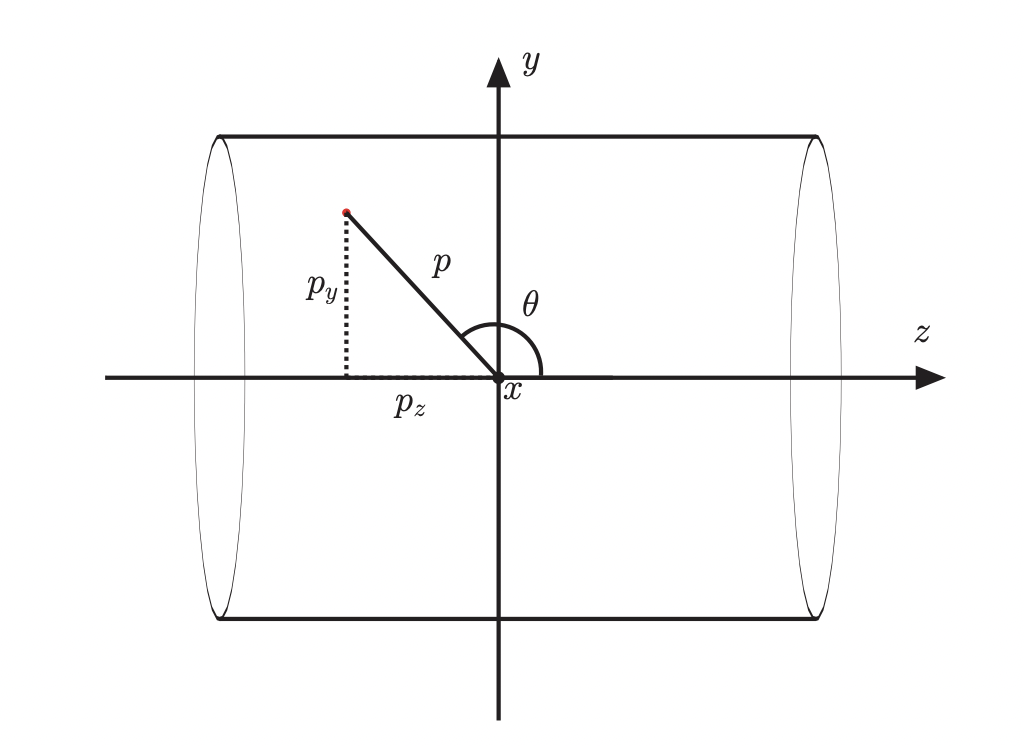
\includegraphics[width=\textwidth]{Figures/atlas/longitudal_plane.png}
        \caption{Longitudal plane of detector}
        \label{fig:longitudal_plane}
    \end{subfigure}
    \hfill
    \caption[ATLAS detector longitudal and azimuthal diagrams]{Spherical coordinate definitions with the azimuthal and polar angles $\phi$ and $\theta$. Here figure \ref{fig:transverse_plane} of the transverse plane shows the z-axis
     into the paper, where as figure \ref{fig:longitudal_plane} of the longitudal plane shows the positive x-axis going out of the paper. Source \href{https://www.duo.uio.no/bitstream/handle/10852/37785/thesis_clean_embedded.pdf?sequence=2&isAllowed=y}{here}. Accessed 16.03.23 }
    \label{fig:long_trans_plane}
\end{figure}

In figure \ref{fig:long_trans_plane} the kinematic variables for proton-proton collisions are described by the energy, rest mass 
and momentum, given as E, m, and $\textbf{p} = (p_x, p_y, p_z)$ respectively. As the particles move with very high energy, we will 
use the relativistic 4 momentum\footnote{In special relativity, 4 momentum is used as both energy and momentum are conserved, and 
thus by creating the 4 momentum, you achieve a Lorentz invariant quantity\cite{Thomson:2013zua}. }, given as $\textbf{P} = (E, \textbf{p})$. We also have that 
\begin{equation*}
    \gamma = \frac{1}{\sqrt{1-\beta^2}},
\end{equation*}
where $\gamma$ is the Lorentz factor, and $\beta = \frac{v}{c}$, which gives us the following definitions for energy $E = \gamma m$ and momentum $\textbf{p} = \beta\gamma m$\cite{Gramstad:1631043}. 
From this we can derive the energy momentum formula:

\begin{align*} 
    \textbf{p}^2 &= \beta^2\gamma^2m^2  \\ 
    \textbf{p}^2 + m^2 &=  m^2(\beta^2\gamma^2 + 1) \\
    \textbf{p}^2 + m^2 &= m^2\gamma^2 \\
    \textbf{p}^2 + m^2 &= E^2
\end{align*}

\begin{equation}\label{eq:energy_momentum}
    E = \sqrt{p^2 + m^2}.
\end{equation}

It can be shown that the phase space of a particle is given by\cite{green_highpt}:

\begin{equation}\label{eq:phase_space}
    d\textbf{p} = dp_xdp_ydp_z = p^2dpd\Omega = dp_zp_Tdp_Td\phi,
\end{equation}

where $p_z$ is the momentum along the beam direction, $p_T$ is the projected momentum on the transverse plane, 
and $\Omega$ is the solid angle. An analog to the relativistic longitudal velocity is the rapidity y. To define this 
we have that the relativistic generalization of equation \ref{eq:phase_space} is given by:
\begin{equation*}
    d^4p\delta (E^2 - p^2 - m^2) = d\textbf{p}\frac{1}{E} = p_T dp_Td\phi dy, \, \, dy = \frac{dp_z}{E}.
\end{equation*}

Using the fact that $p = \sqrt{p_T^2 + p_z^2}$ and equation \ref{eq:energy_momentum} we can integrate $dy$ to get the rapidity:

\begin{equation*}
    \int dy = \int \frac{dp_z}{\sqrt{p_T^2 + p_z^2 + m^2}}
\end{equation*}

\begin{equation}
    y = \cosh^{-1}\left( \frac{E}{\sqrt{p_T^2 + m^2}}\right)
\end{equation}

For particles with little to no mass relative to the transverse momentum, we have that $p_T^2 + m^2 \approx p_T^2$ 
where $p_T = E\sin{(\theta)}$, which gives us the following relations:

\begin{equation*}
    \cosh(y) = \frac{1}{\sin(\theta)},
\end{equation*}
\begin{equation*}
    \sinh(y) = \frac{1}{\tan(\theta)},
\end{equation*}
\begin{equation*}
    \tanh(y) = \cos(\theta).
\end{equation*}

which can be used to show that $e^{-y} = \tan{\frac{\theta}{2}}$. From this we define the pseudorapidity $\eta$ as:
\begin{equation}
    \eta = -\ln{\left( \tan{\frac{\theta}{2}}\right)},
\end{equation}
which is, in the relativistic limit, the same as the rapidity y. A useful property of the pseudorapidity is that 
the phase space of a single particle is uniformly distributed for both $\eta$ and $\phi$, making them good features 
to compare overlap between SM MC and ATLAS data\cite{Gramstad:1631043}. 
\subsection*{Data collection}

\begin{figure}[H]
    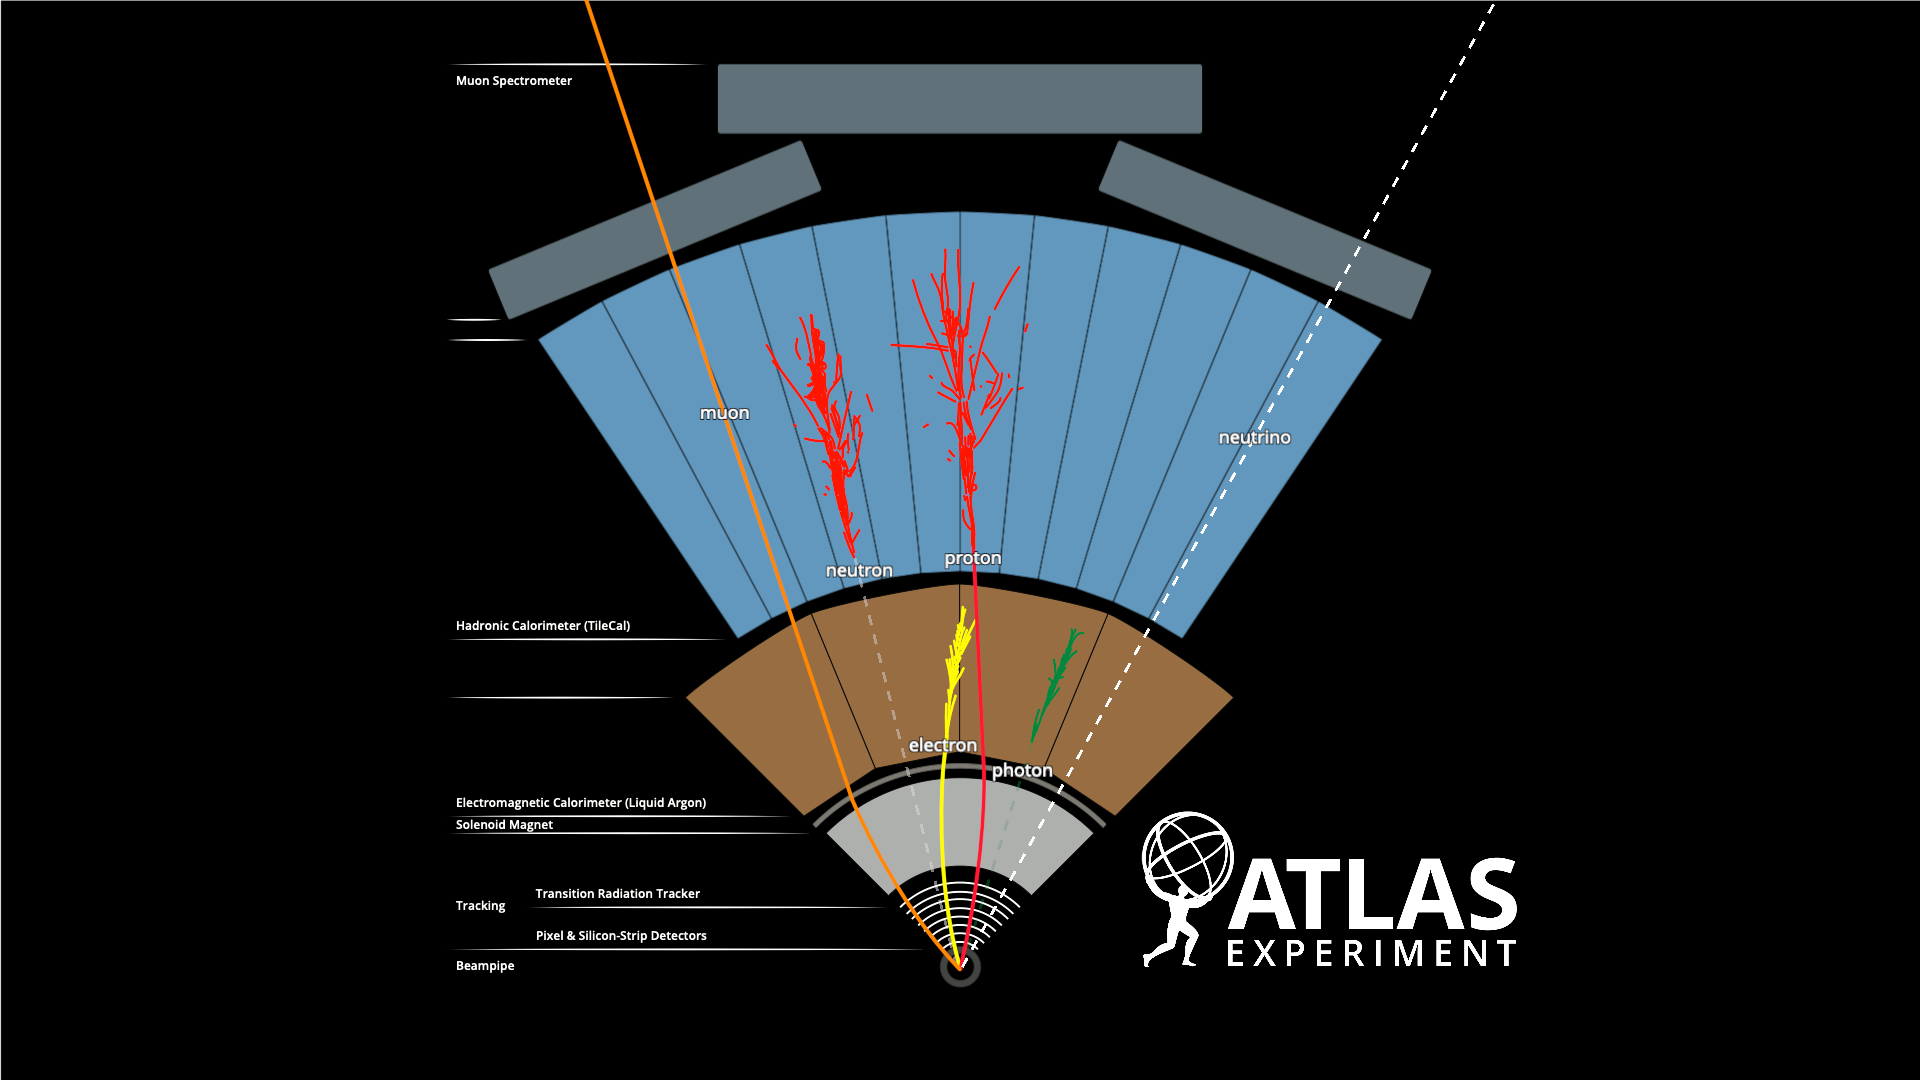
\includegraphics[width=\linewidth]{Figures/atlas/ATLAS Detector Schematic black particles.png}
    \caption[Detector tracking of particles]{Figure describing how particles are detected at ATLAS, fetched from \href{https://cds.cern.ch/record/2770815}{	ATLAS detector slice (and particle visualisations)}, by Sascha Mehlhase \cite{Mehlhase:2770815} . }
    \label{fig:atlas_particle_detect}
\end{figure}

The features used in this analysis are computed with or fetched from the features from the 
detector itself. Such features include the momentum, energy, angles etc., 
all of which are either directly measured or computed based on the measurements in the 
detector. In figure \ref{fig:atlas_particle_detect} a visualization shows how
different particles move through the detector and how they are detected. For example, 
energy deposits are measured using calorimeters, and the different particles 
have calorimeters specially designed for them. Charged particles leave tracks in the 
inner tracking device. Thus, electrons leaves tracks in the inner tracker and deposits energy 
in the elctromagnetic calorimeter, the muons leaves tracks in the inner detector and 
deposits energy in the muon detector. The photons only deposits energy in the electromagnetic 
calorimeter. Hadrons like protons and neutrons deposits energy in the electromagnetic and 
hadronic calorimeters, and charged hadrons also leaves tracks in the inner tracker. This is 
shown in figure \ref{fig:atlas_particle_detect}.\par

The ATLAS detector have a few thousand selection stages before the data is stored. 
In order to reach the highest intensity of collisions, the LHC accellerates
packets of around $10^{11}$ protons, and collides them at a rate of 25 nanoseconds, 
yeilding a collision rate of 40 MHz\cite{Wang:2707056}. \cite{Bernius:2707054}



\subsubsection*{Data preparation}
During datagathering at the ATLAS detector, triggers on the hardware and software level select out the events that are of most interest. On the order of $99 \%$ or
 more of the recorded events are discarded, with about 1 in 40000 events being accepted, as the amount of recorded events simply as too high to realistically analyse. Also, a lot of the events are of no 
 interest for new physics analysis anyway as they for example might have too little energy. Once the trigger selection is done, the data is reconstructed. This means that the objects
 in the recorded events are through software algorithms reconstructed into particles, jets, photons etc. The reconstruction is done based on the tracks and measurements
 in the detector, but it is not perfect, and can lead to fake leptons or jets. By fake, it is meant that an object might look like a lepton but is in reality a jet or vice versa\cite{Gillam:2015kta}.
 Once the reconstruction is done, further slimming of the n-tuples are done. Derivations are slimmings of the n-tuples where the selection of events are further reduced 
 to match the needs of the different analysis groups. \par 
The SM MC go through parts of the same process. These events are first generated and then run through the detector to simulate actual events. Once that is done, the events
 can be reconstructed and go through derivations just like the pp-collision data, to be used in analysis. 

\begin{figure}[H]
    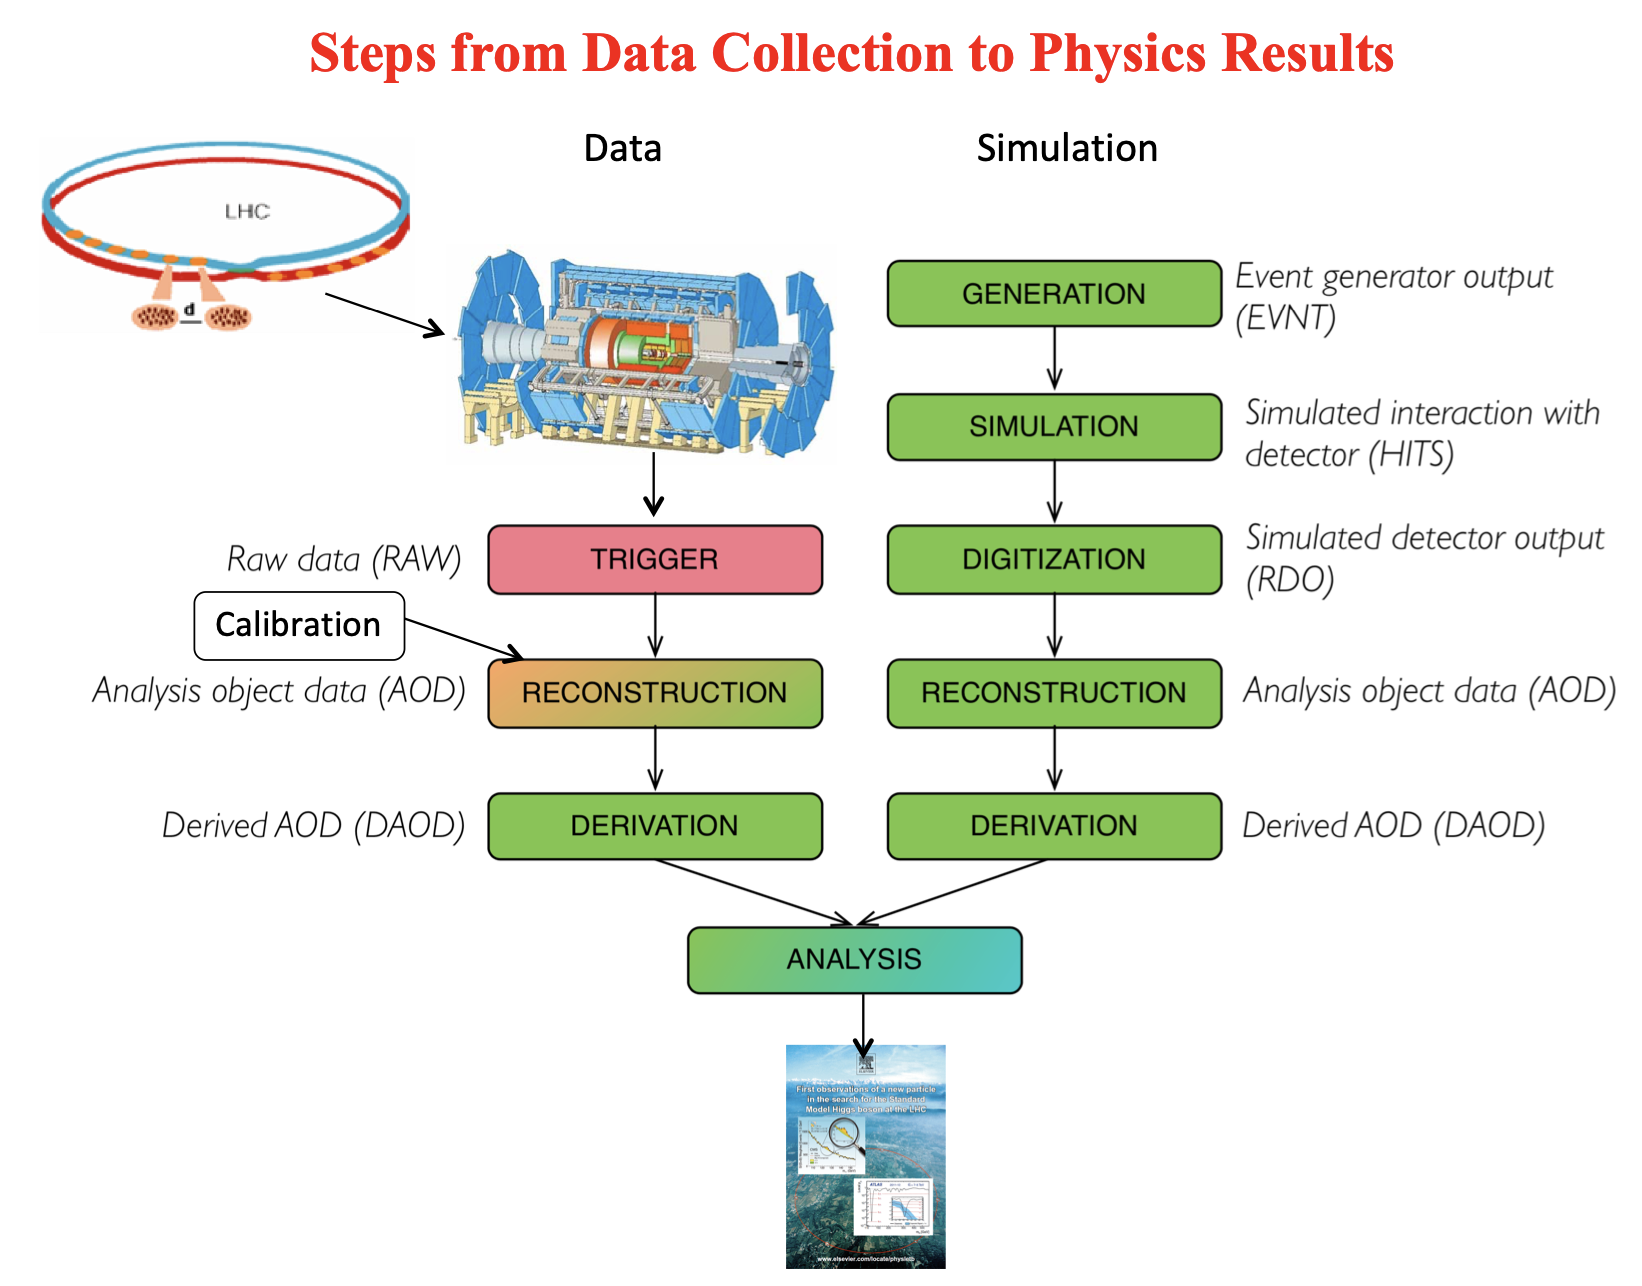
\includegraphics[width=\linewidth]{Figures/atlas/data_col_phys.png}
    \caption[Steps from data collection to physics results]{Figure describing the steps to take for data collection at ATLAS, fetched from \href{https://indico.cern.ch/event/1159574/timetable/?view=standard}{Hybrid ATLAS Induction Day + Software Tutorial workshop}, part
    \href{https://indico.cern.ch/event/860971/contributions/3672974/attachments/1972049/3280896/Atlas_computing_data_preparation_jan20.pdf}{Computing and Data preparation}, 
    held by S.M Wang \cite{Wang:2707056} . }
    \label{fig:atlas_data_col_phys}
\end{figure}


\subsubsection*{Jets}
Photons and electrons are detected in the electromagnetic calorimeter, and are easy to track and detect as they 
separate easily. Quarks, however, are bound by QCD and thus cannot be seperated as individual 
particles. An illustration of how quarks and gluons materialise as jets during a proton-proton 
collision is shown below in figure \ref{fig:cms_jets}.

\begin{figure}[H]
    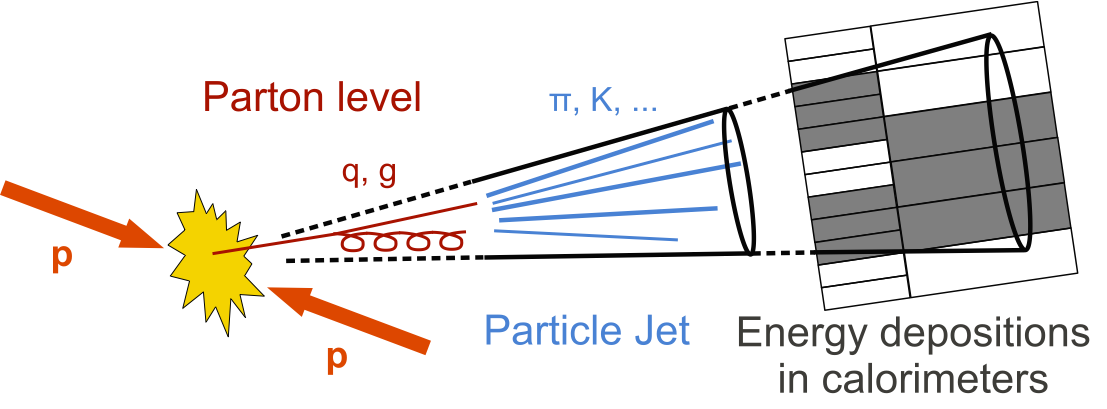
\includegraphics[width=\linewidth]{Figures/atlas/cms_Sketch_PartonParticleCaloJet.png}
    \caption[Jet produciton from pp-collisions to detector]{Figure describing how quarks and gluons are treated in the detector, and thus why we name them jets, fetched from \href{https://cms.cern/sites/default/files/field/image/Sketch_PartonParticleCaloJet.png}{the CMS webpage}. }
    \label{fig:cms_jets}
\end{figure}

In a proton-proton collision, the quarks and gluons forms stable or unstable hadrons such that the color confinement\footnote{Add link to a source or explanation for this.} is upheld. These then 
decay to other stable hadrons that can be tracked, and these tracks are called jets. This is particularly difficult because one wants to isolate which hadrons came from  the original quark in the 
Feynman diagram. Another point to make is that some quarks are of higher interest than others. For example, the b jet, coming from a b quark, is a good indicator for certain processes, 
thus identifying suchs particles is of huge interest. 
\section{ROOT}
ROOT is an open-source data analysis framework used by high energy physics. It can do fast data manipulation, save and access data, 
create graphics for publication, and even combine with high level languanges such as R and Python.


\subsection*{RDataFrame}
RDataFrame's main purpose is to make reading and handling of ROOT files easier, especially in 
relation to modern machine learning tools and their respective frameworks and environments. 
This is done by creating a dataframe type of structure of the ROOT n-tuples, and then 
lazily\footnote{In this context lazily means that the functions and or cuts are done first after 
all have been registered, see \href{https://root.cern/doc/master/classROOT_1_1RDataFrame.html}{ROOT 
guidelines} for more.} apply contraints to the data. Using PyROOT
\footnote{\href{https://root.cern/manual/python/}{PyROOT website}}, RDataFrame can be accessed in 
Python, as the functionality is wrapped around a C++ class. Below is a code example of how
to create a RDataFrame object, apply a cut and then create a column for later use. Here, good 
leptons are defined first, denoted as "ele\_SG" and "muo\_SG". A cut is then applied where we 
require that the number of good leptons is always 3. Finally, a column is created where the 
combination of type of leptons in the 3 lepton system is stored, as well as creating a histogram 
containing the results for that given channel\footnote{A channel here refers to a certain decay 
channel. The simulations of the SM is divided into several channels, and some look more alike than others. One example is 
the Higgs decay channel, with possible decays such as two photons, W bosons or Z bosons. This pertains 
to simulated events only, as we cannot control what decay channels we get in the data recorded at ATLAS} 
k. Notice here that if the variable already exists as a column in the dataframe, arithmetic and logic 
can be applied directly using those columns to create new one. More complicated variables, such as 
the flavor combination for the leptons, or the invariant mass of two particles must be found or 
calculated using C++ functions. An example of such a C++ function is shown below the python code example. 

\begin{figure}[H]
    \centering
\begin{lstlisting}[language=Python, style=pythonstyle, label={code:python_func_example}]
import ROOT as R

R.EnableImplicitMT(200)
R.gROOT.ProcessLine(".L helperFunctions.cxx+")
R.gSystem.AddDynamicPath(str(dynamic_path))
R.gInterpreter.Declare(
    '#include "helperFunctions.h"'
)  # Header with the definition of the myFilter function
R.gSystem.Load("helperFunctions_cxx.so")  # Library with the myFilter function

df_mc = getDataFrames(mypath_mc)
df_data = getDataFrames(mypath_data)
df = {**df_mc, **df_data}

for k in df.keys():

    # Signal leptons
    df[k] = df[k].Define(
        "ele_SG",
        "ele_BL && lepIsoLoose_VarRad && lepTight && (lepD0Sig <= 5 && lepD0Sig >= -5)",
    )  
    df[k] = df[k].Define(
        "muo_SG",
        "muo_BL && lepIsoLoose_VarRad && (lepD0Sig <= 3 && lepD0Sig >= -3)",
    )  
    df[k] = df[k].Define("isGoodLep", "ele_SG || muo_SG")
    df[k] = df[k].Define(
                "nlep_SG", "ROOT::VecOps::Sum(ele_SG)+ROOT::VecOps::Sum(muo_SG)"
            )

    df[k] = df[k].Filter("nlep_SG == 3", "3 SG leptons")

    # Define flavor combination based on 
    df[k] = df[k].Define("flcomp", "flavourComp3L(lepFlavor[ele_SG || muo_SG])")
    histo[f"flcomp_{k}" ] = df[k].Histo1D(
        (
            f"h_flcomp_{k}",
            f"h_flcomp_{k}",
            len(fldic.keys()),
            0,
            len(fldic.keys()),
        ),
        "flcomp",
        "wgt_SG",
    )
    \end{lstlisting}
    \caption[RDataFrame code example]{Example of event selection done using RDataFrame.}
    \label{code:rdata}
\end{figure}

In the code example above we see how RDataframe can be used for event selection. Line 1-9 are settings for ROOT, 
number of threads to use in the paralellization, extra helper functions written in C++ with .h and .so files and the path to the folder.
Lines 11-13 create a dictionary containing the ROOT RDataFrames used for event selection. These are categorized by channel name. 
The loop on line 15 does event selection for each channel sample, defining new variables in the RDataFrame, applying filters and creating histograms.
Some variables are constructed using variables already in the ROOT files such as energy and mass. Through custom C++ functions
these properties can be added to the RDataFrames. The example below shows a custom C++ function which is used in work of this thesis.

\begin{figure}[H]
    \centering
\begin{lstlisting}[language=C++, style=cppstyle, label={code:cpp_func_example}]
double getM(VecF_t &pt_i, VecF_t &eta_i, VecF_t &phi_i, VecF_t &e_i,
            VecF_t &pt_j, VecF_t &eta_j, VecF_t &phi_j, VecF_t &e_j,
            int i, int j)
{
    /* Gets he invariant mass between two particles, be it jets or leptons */

    const auto size_i = int(pt_i.size());
    const auto size_j = int(pt_j.size());

    if (size_i == 0 || size_j == 0){return 0.;}
    if (i > size_i-1){return 0.;}
    if (j > size_j-1){return 0.;}

    TLorentzVector p1;
    TLorentzVector p2;

    p1.SetPtEtaPhiM(pt_i[i], eta_i[i], phi_i[i], e_i[i]);
    p2.SetPtEtaPhiM(pt_j[j], eta_j[j], phi_j[j], e_j[j]);

    double inv_mass = (p1 + p2).M();

    return inv_mass;
}
\end{lstlisting}
\caption[C++ function example]{Example of a C++ function used in event selection.}
\end{figure}
This C++ function creates Lorentz vectors for two particles, and then returns the invariant mass based on the parameters sent in. 
This function will be used on all the leptons in a given event. If one particle or both do not exist, the C++ function will
return zero as the invariant mass. \par


\begin{figure}[H]
    \centering
\begin{lstlisting}[language=Python, style=pythonstyle, label={code:python_func_example_2}]
import pandas as pd 

cols = df.keys()

for k in cols:

    print(f"Transforming {k}.ROOT to numpy")
    numpy = df[k].AsNumpy(DATAFRAME_COLS)
    print(f"Numpy conversion done for {k}.ROOT")
    df1 = pd.DataFrame(data=numpy)
    print(f"Transformation done")
    

    df1.to_hdf(
        PATH_TO_STORE + f"/{k}_3lep_df_forML_bkg_signal_fromRDF.hdf5", "mini"
    )

\end{lstlisting}
\caption[Conversion from RDataFrame to NumPy]{Loop converting RDataFrames to NumPy structures, before being stored as HDF5 files.}
\end{figure}

Once event selection is done, the features have been chosen and histograms have been 
drawn, the RdataFrame can be converted to a Pandas dataframe. This is a very popular 
choice for data structure when doing data analysis in python. This is done through an 
intermediary step of converting the RDataframe to a numpy filestructure, which then can 
be converted to a Pandas\cite{reback2020pandas} dataframe or some other framework.
The new Pandas dataframes are stored as HDF5\cite{hdf5} files to be used later. This is 
because the HDF5 format has a very good compression ratio, and is very fast to read and write. 
\section{Background samples}

\subsection*{3 lepton background MonteCarlo}
To look for the heavy neutrinos, we need to train on background MonteCarlo with that finalstate aswell. This means in a sense that 
we want the autoencoder to learn what is expected from the Standard model in terms of this final state. The 3 lepton background MonteCarlo 
contains the following channels:

\begin{enumerate}
    \item Wjets
    \item Triboson
    \item Higgs
    \item Zttjets
    \item Zmmjets
    \item Zeejets
    \item SingleTop
    \item TopOther
    \item ttbar
    \item Diboson2L
    \item Diboson3L
    \item Diboson4L
\end{enumerate}

Below are three examples of what some of the samples contains. The selected ones are likely Feynman diagrams for $t\bar{t}$, Higgs and Zeejets channels. 

\begin{figure}[h!]
    \centering
    \caption{Proton-proton collision showing the $t\bar{t}$ channel. Here the w bosons decay leptonically and one or more jets
    are misreconstructed as leptons by the detector. }

\begin{tikzpicture}
    \begin{feynman}
    
        \vertex at (0, 1.) (a2){\(g\)} ;
        \vertex at (0, -1.)  (a5){\(g\)} ;

        \vertex at (1.5, 1.) (c);
        \vertex at (3., 1.) (d);

        \vertex at (1.5, -1.) (e);
        \vertex at (3., -1.) (f);

        \vertex at (1.5, 1.) (g);
        \vertex at (1.5, -1.) (h);

        \vertex at (3, 1) (a1);
        \vertex at (4.5, 1.5) (a3);

        \vertex at (3, 1) (a6);
        \vertex at (4.5, 0.5) (a7);


        \vertex at (3, -1) (b1);
        \vertex at (4.5, -1.5) (b2);

        \vertex at (3, -1) (b3);
        \vertex at (4.5, -0.5) (b4);

       
        
    \diagram*{


        (a2) -- [gluon] (c) -- [anti fermion, edge label = {$\bar{t}$}] (d),
    
        (a5) -- [gluon] (e) -- [fermion, edge label = {$t$}] (f),

        (g) -- [fermion, edge label = {$t$}] (h),

        (a1) -- [boson, edge label ={$w^-$}] (a3),

        (a6) -- [anti fermion, edge label ={$\bar{b}$}] (a7),

        (b1) -- [boson, edge label ={$w^+$}] (b2),

        (b3) -- [anti fermion, edge label ={$b$}] (b4),
        
        ;
    };
    \end{feynman}
    \end{tikzpicture}
    \label{fig:ttbar_feynman}
    \end{figure}

    \begin{figure}[h!]
        \centering
        \caption{Proton-proton collision showing the Higgs channel. Here the Z bosons decay leptonically. }
    
    \begin{tikzpicture}
        \begin{feynman}
        
            \vertex at (0, 1.) (a2){\(g\)} ;
            \vertex at (0, -1.)  (a5){\(g\)} ;
    
            \vertex at (1.5, 1.) (c);
            \vertex at (3., 0) (d);
    
            \vertex at (1.5, -1.) (e);
            \vertex at (3., 0) (f);
    
            \vertex at (1.5, 1.) (g);
            \vertex at (1.5, -1.) (h);
    
            \vertex at (3, 0) (a1);
            \vertex at (4.5, 0) (a3);

            \vertex at (6, 1) (a6);
            \vertex at (6, -1) (a7);
    
           
            
        \diagram*{
    
    
            (a2) -- [gluon] (c) -- [anti fermion, edge label = {$\bar{t}$}] (d),
        
            (a5) -- [gluon] (e) -- [fermion, edge label = {$t$}] (f),
    
            (g) -- [fermion] (h),
    
            (a1) -- [dashed, edge label = {$H$}] (a3),

            (a3) -- [boson, edge label = {$Z$}] (a6),
            (a3) -- [boson, edge label = {$Z$}] (a7),


            
            ;
        };
        \end{feynman}
        \end{tikzpicture}
        \label{fig:higgs_feynman}
        \end{figure}
        
        \begin{figure}[h!]
            \centering
            \caption{Proton-proton collision showing the Zeejets channel. Here one of the Z bosons decay leptonically and the W boson
            decays hadronically. }
        
        \begin{tikzpicture}
            \begin{feynman}
                \vertex at (0, 1.) (a2){\(q\)} ;
                \vertex at (0, -1.)  (a5){\(\bar{q}^{'}\)} ;

                \vertex at (1.5, 1.) (c);

                \vertex at (1.5, -1.) (e);

                \vertex at (3, 1.) (b1);

                \vertex at (3, -1.) (b2);

                \vertex at (4.5, -0.5) (b4);

                \vertex at (4.5, -1.5) (b3);

                \vertex at (4.5, 0.5) (b5);

                \vertex at (4.5, 1.5) (b6);
        
                
               
                
            \diagram*{
        
        
                (a2) -- [fermion] (c),
            
                (a5) -- [anti fermion] (e),

                (c) -- [fermion] (e),

                (c) -- [boson, edge label={$Z$}] (b1),
                (e) -- [gluon, edge label={$g$}] (b2),

                (b2) -- [fermion, edge label={$b$}] (b4),
                (b2) -- [anti fermion, edge label={$\bar{b}$}] (b3),

                (b1) -- [fermion, edge label={$e^-$}] (b5),
                (b1) -- [anti fermion, edge label={$e^+$}] (b6),
        
                ;
            };
               
            \end{feynman}
            \end{tikzpicture}
            \label{fig:zeejets_feynman}
            \end{figure}

\subsection*{2 lepton background MonteCarlo}

\begin{enumerate}
    \item singletop 
    \item Diboson 
    \item Zeejets 
    \item Zmmjets 
    \item Zttjets 
    \item Wjets 
    \item ttbar
   
\end{enumerate}

 
\section*{The dataset features}

\subsection*{RMM matrix}
Most of the features in the analysis are elements in the so called Rapidity-Mass (RMM) matrix inspired by the work of Chekanov \cite{Chekanov_2019}.
\par
!! Motivation for using such a matrix in machine learning $\to$ hint to highly uncorrolated feats!!
\par
Its composition is determined as a square matrix of $1 + \sum_{i=1}^{T}N_i$ columns and rows, where T is the total number of objects (i.e jets, electrons etc.),
and $N_i$ is the multiplicity of a given object. In the case of the same number of a given object for all objects, we can denote the RMM matrix as a 
TmNn matrix, where m is the multiplicity of T, and n is the number of particle per type. Thus there is already room for evaluation, as the combination of number of objects 
and the number of each object type highly affects the analysis as well as computational resources. Each cell in the matrix contains information about
either single og two particle properties. An example is shown in matrix \ref{eq:rmmmatrix}.

\begin{equation}\label{eq:rmmmatrix}
\begin{pmatrix}
    \boldsymbol{e}_{T}^{miss} & m_T(j_1) & m_T(j_2) &  m_T(e_1) &  m_T(e_2)\\
    h_L(j_1) & \boldsymbol{e_T}(j_1) & m(j_1, j_2) & m(j_1, e_1) & m(j_1, e_2)\\
    h_L(j_2) & h(j_2, j_1) & \delta \boldsymbol{e_T}(j_2)& m(j_2, e_1) & m(j_2, e_2)\\
    h_L(e_1) & h(e_1, j_1) & h(e_1, j_2) & \boldsymbol{e_T}(e_1) & m(e_1, e_2)\\
    h_L(e_2) & h(e_2, j_1) & h(e_2, j_2) & h(e_2, e_1) & \delta \boldsymbol{e_T}(j_2)\\
\end{pmatrix}
\end{equation}

In matrix \ref{eq:rmmmatrix} we have the RMM matrix for a T2N2 system, in other words we have two types of particles, jets and electrons, where each type has
two particles. The matrix itself is partitioned into three parts. The diagonal represents energy properties, the upper triangular represents mass properties, 
and the lower triangular represents longitudal properties related to rapidity. The diagonal has three different properties, $\boldsymbol{e_T^{miss}}$, $\boldsymbol{e_T}$ and $\delta\boldsymbol{e_T}$. 
$\boldsymbol{e_T^{miss}}$ is placed in the $(0,0)$ in the matrix. It accounts for the missing energy for the system, which is of high interest for this analysis due to
the search for heavy neutrinos. $\boldsymbol{e_T}$ is the transverse energy defined as 
\begin{equation*}
    \boldsymbol{e_T} = \sqrt{m^2 + p_T^2}
\end{equation*}
but for light particles such as electrons, this can be approximated to $\boldsymbol{e_T} \approx p_T$. $\delta\boldsymbol{e_T}$ is the transverse energy imbalance.
It is defined as 
\begin{equation*}
    \delta\boldsymbol{e_T} = \frac{E_T(i_n-1) - E_T(i_n)}{E_T(i_n-1) + E_T(i_n)}, \, n = 2, ..., N.
\end{equation*}
The first columm in the RMM matrix, with the exeption of the first element, is related to the longitudal property of the given particle. 
It is defined as
\begin{equation*}
    h_L(i_n) = C(\cosh{(y)} - 1),
\end{equation*}
where C is a constant to ensure that the average $h_L(i_n)$ values do not deviate too much from the ranges of the invariant masses of the transverse masses, found to be $0.15$\cite{Chekanov_2019}. 
y is the rapidity of the particle, and $i_n$ is the particle number. On the lower triangle we have the longitudal properties of the combinations of particles. Similar to $h_L(i_n)$,
this property is defined as 
\begin{equation*}
    h(i_n, j_k) = C(\cosh{(\Delta y)} - 1),
\end{equation*}
where $\Delta y = y_{i_n} - y_{j_k}$ is the rapidity difference for particle $i_n$ and $j_k$.


\subsection*{MonteCarlo and data comparison}\label{sec:mcdatacomp}

Before we can start the analysis, we need to compare the MonteCarlo and data. This is done to ensure that the training samples we use are actually useful. As described by R. Stuart 
Geiger et al. \cite{DBLP:journals/corr/abs-2107-02278}, the concept of "Garbage in, garbage out" is of key importance in computer science, and indeed important in high energy physics. 
To ensure that the models we train actually learns physical processes, the training set must represent the physics "status quo". If the training samples do not match the physical reality,
we regard it, in the context of high energy physics, as garbage in, which will in turn give garbage out. The Monte Carlo standard model simulations are indeed very good, but the are 
numerical approximations, and can sometimes be off. Thus, every feature that well be used for training have to be checked before being used. This is done by comparing the distributions 
of the features in the MonteCarlo and ATLAS data. Assuming that there are no issues with the data collection from ATLAS, we then assume that the data from ATLAS is the "ground truth", as it 
is the only dataset we can analyze, and the only dataset we can compare to. The MonteCarlo is then compared to the data, and if the distributions are similar, we can assume that the 
training samples are good enough. 


\begin{figure}
    \centering
    \begin{subfigure}{.6\textwidth}
        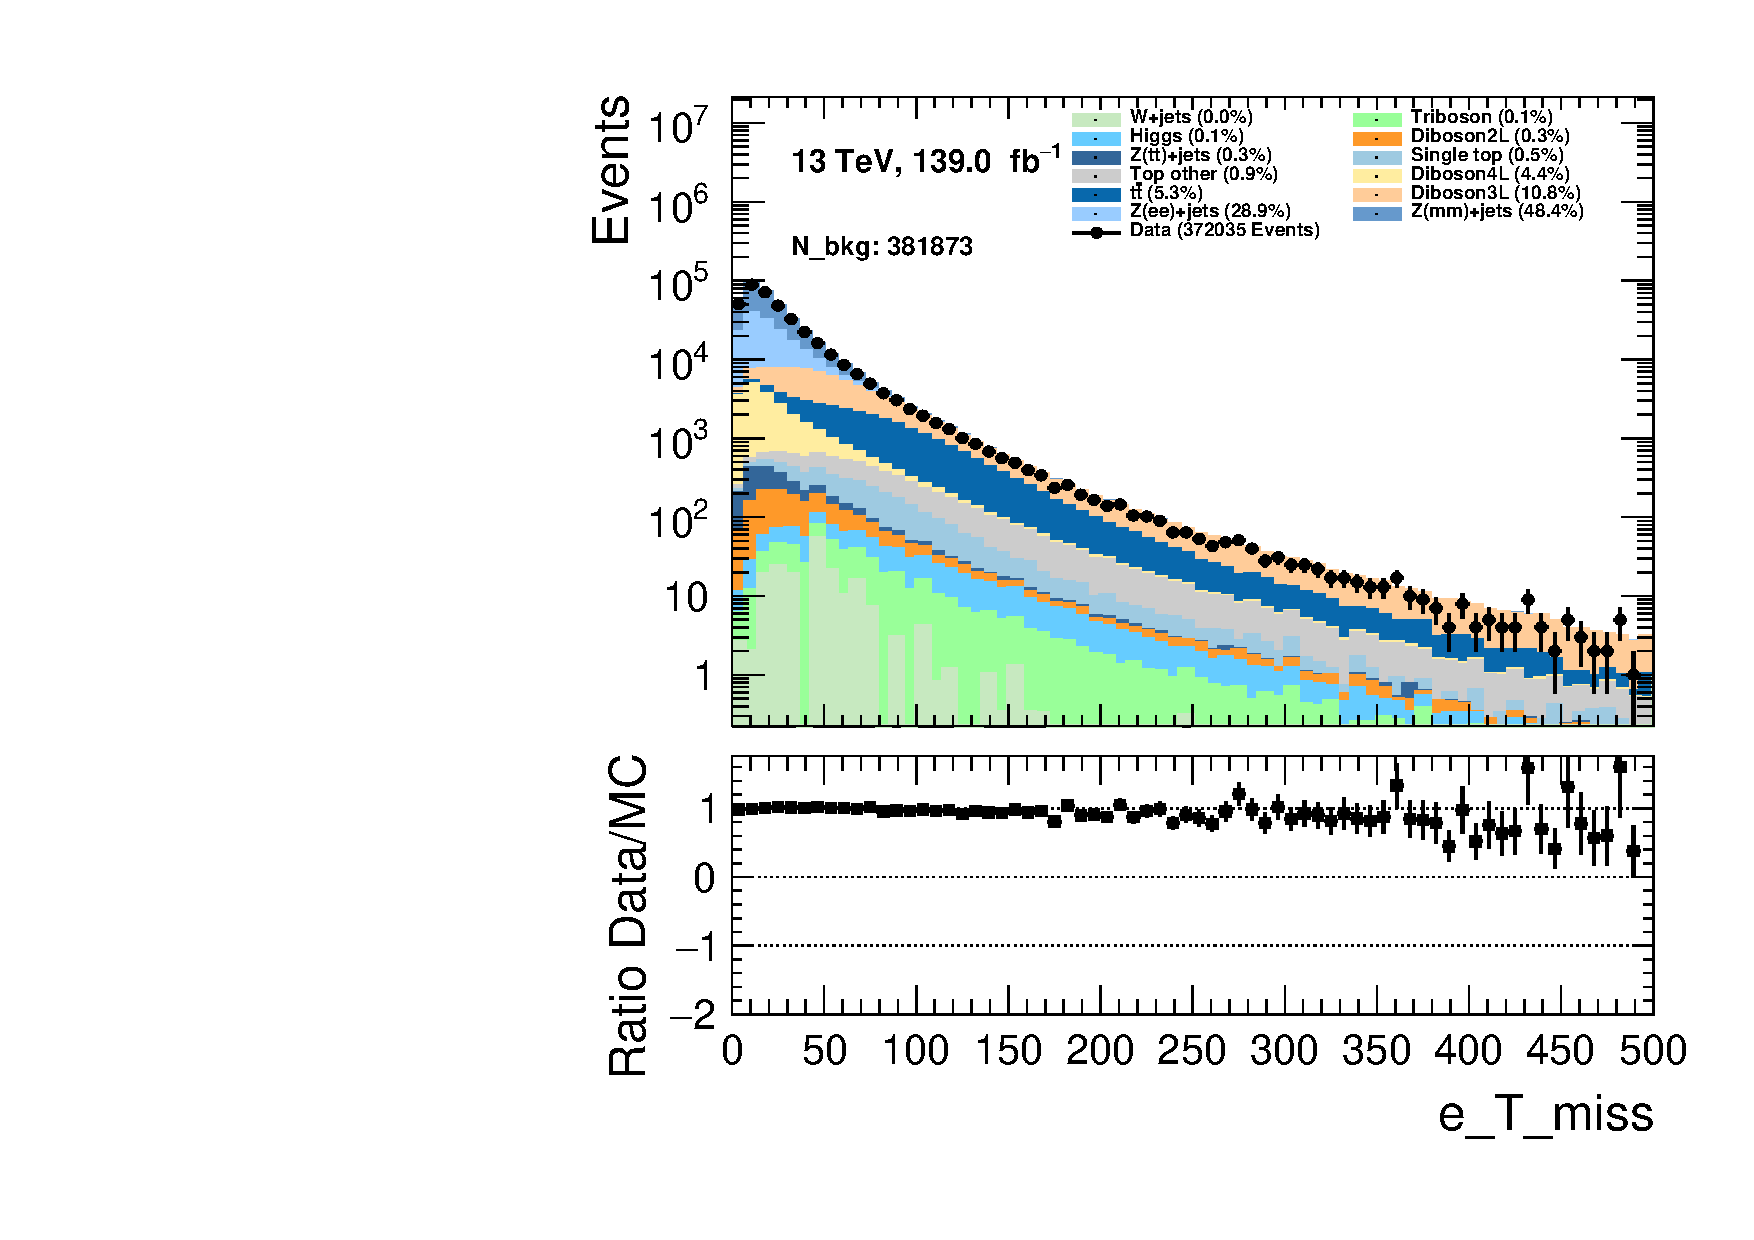
\includegraphics[width=\textwidth]{Figures/MC_Data_comp/e_T_miss.pdf}
        \caption{Missing transverse energy for the three lepton final state. The histogram contains the entire Run 2 dataset.}
        \label{fig:etmiss}
    \end{subfigure}
    \hfill
    \begin{subfigure}{.6\textwidth}
        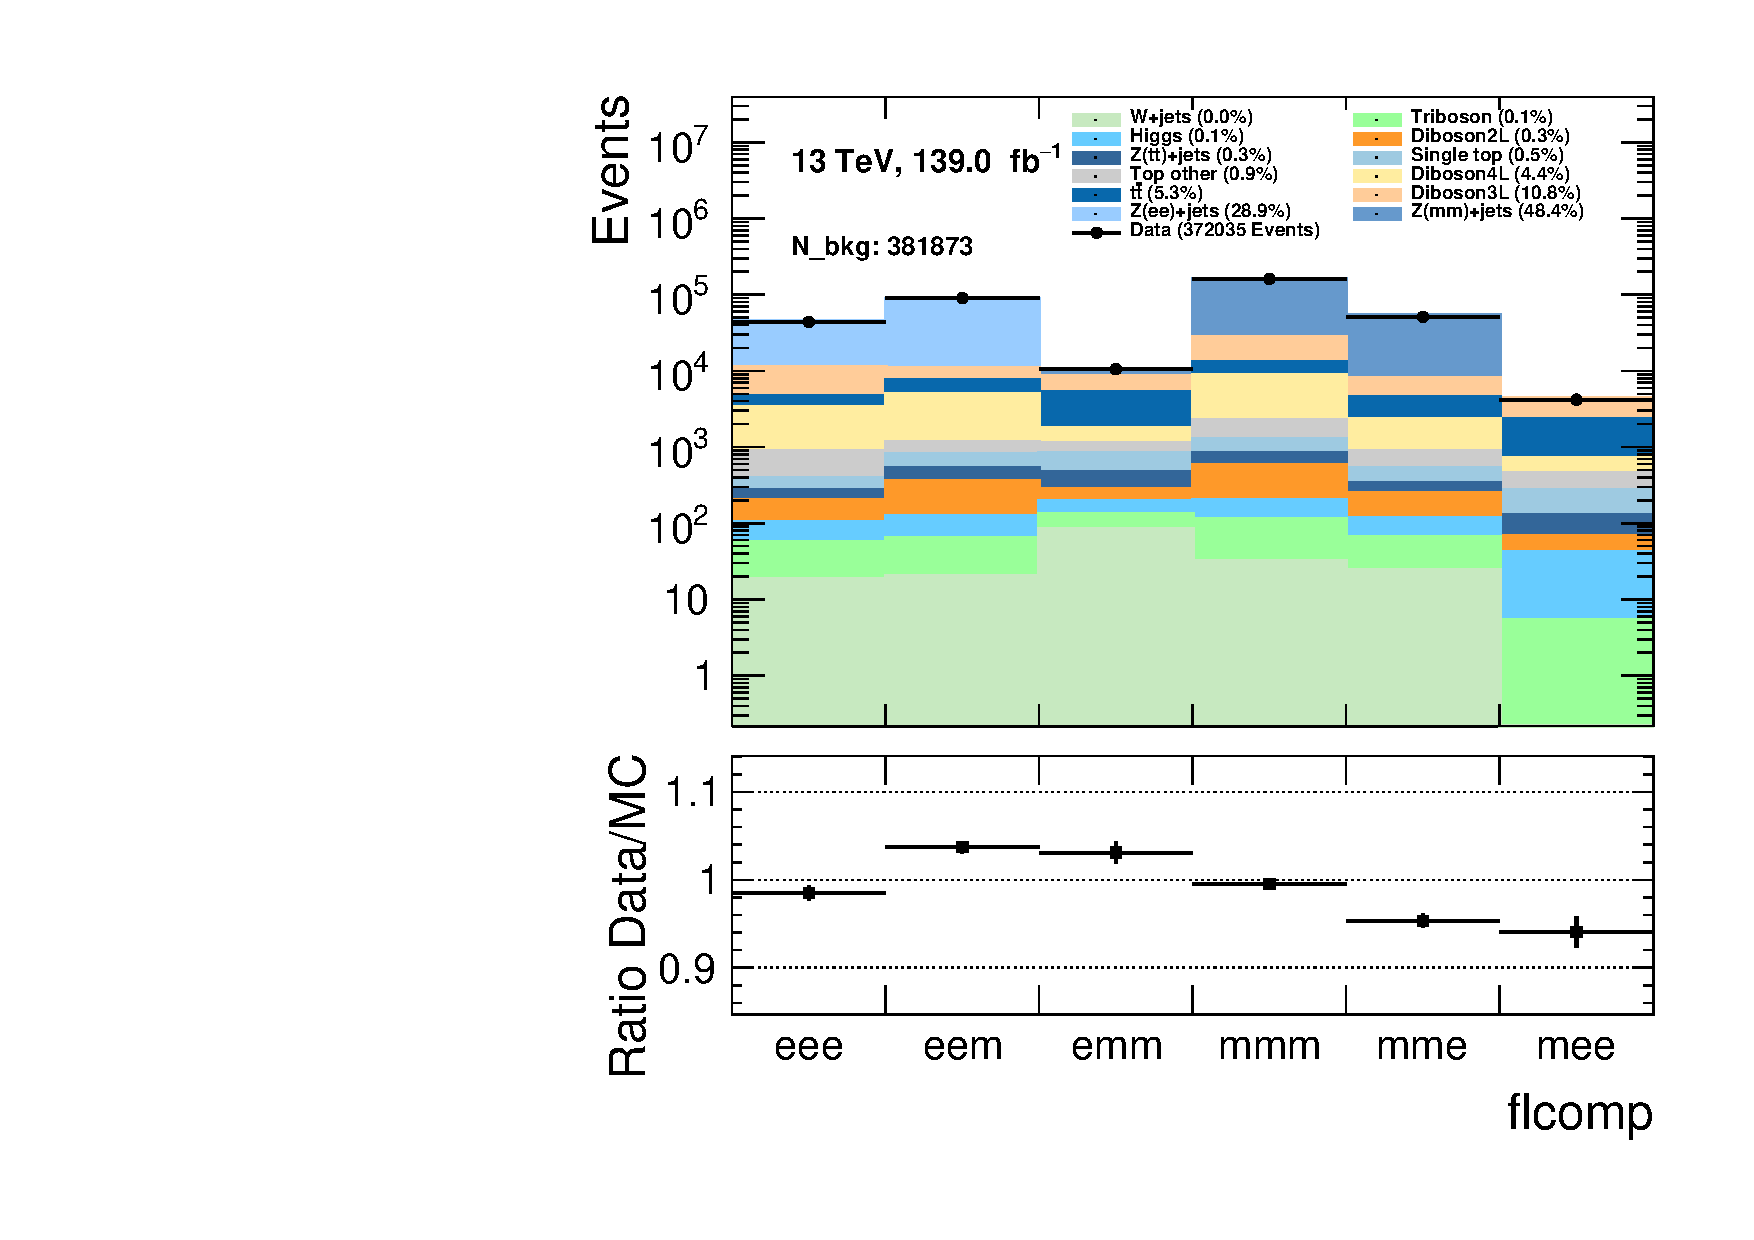
\includegraphics[width=\textwidth]{Figures/MC_Data_comp/flcomp.pdf}
        \caption{Flavor combination for the three lepton final state. This histogram only contains the flavor combinations for the good leptons, denoted $lep_{SG}$. The histogram contains the entire Run 2 dataset. }
        \label{fig:flcomp}
    \end{subfigure}
    \hfill        
    \caption{Comparison of the MonteCarlo and data for the three lepton final state with the features $e_{T}^{miss}$ and flavor composition.
    }
    \label{fig:MC_Data_comp}
\end{figure}

In figure \ref{fig:MC_Data_comp} two features have been selected to vizualize the comparison between Monte Carlo and ATLAS data, $e_T^{miss}$ and $flcomp$. 
We see that both $e_T^{miss}$ and $flcomp$ satisfy a good ratio between Monte Carlo and ATLAS data, thus we can safely move forward with the analysis. 
All features were checked, and can be found in appendix B.
\par \par

\subsection*{Tabular data}
\section*{Code implementation}

The machine learning analysis was written with Keras\cite{chollet2015keras} using the Tensorflow api\cite{tensorflow2015-whitepaper} . 
The machine learning structure was written using a functional structure\footnote{Functional structure uses a function call for layers, i.e for layers a,b, then b(a) will connect the two layers, and equals a sequential link a $\to$ b. This allows for more flexible structures. More on the functional api can be found \href{https://www.tensorflow.org/guide/keras/functional}{here}.}
In practise, this model could just as well have been written as a Sequential model\footnote{Sequential structure adds layers in sequence, i.e for layers a, b, c we have that a $\to$ b $\to$ c, with a strict structure. This allows for more organized code. More on sequential models can be found \href{https://www.tensorflow.org/guide/keras/sequential_model}{here}.}, 
but at a cost of flexibility and lack of potential non-linear structure in the architecture.\par


%Tuning \cite{omalley2019kerastuner}, \par 
%Tuning optimization \cite{hyperband:opt}, \par
%Optimizing \cite{ADAM:opti}, \par 
%Splitting and scaling \cite{scikit-learn}, \par
%Plotting \cite{Hunter:2007}, \par
%More plotting  \cite{Waskom2021}, \par
%Even more plotting \cite{plotly}, \par
%Arrays \cite{harris2020array}, \par 
%Dataframe structure \cite{reback2020pandas}, \par


\subsection*{Construction of a neural network in Tensorflow}

Using the functional structure, a general neural network in the Tensorflow API can be constructed as shown below. 
\begin{lstlisting}[language=Python, style=pythonstyle, label={code:python_func_example_general}]
import tensorflow as tf


inputs = tf.keras.layers.Input(shape=data_shape, name="input")

# First hidden layer
First_layer = tf.keras.layers.Dense(
    units=30,
    activation="relu"
)(inputs)

# Second hidden layer
Second_layer = tf.keras.layers.Dense(
    units=45, 
    activation="relu"
)(First_layer)

# Second hidden layer
output_layer = tf.keras.layers.Dense(
    units=1, 
    activation="sigmoid"
)(Second_layer)


# Model definition
nn_model = tf.keras.Model(inputs, output_layer, name="nn_model")

hp_learning_rate = 0.0015
optimizer = tf.keras.optimizers.Adam(hp_learning_rate)
nn_model.compile(loss="mse", optimizer=optimizer, metrics=["mse"]) 
\end{lstlisting}
The neural network here contains one input layer, two hidden layers, and an output layer. The choice of nodes and activation functions are 
arbitrary here as the use case has not been defined. Note that this is exactly the same as this example, using a sequential structure.


\begin{lstlisting}[language=Python, style=pythonstyle, label={code:python_seq_example}]
import tensorflow as tf

nn_model = tf.keras.Sequential(
    [
        tf.keras.layers.Dense(30, activation="relu", input_shape=data_shape),
        tf.keras.layers.Dense(45, activation="relu"),
        tf.keras.layers.Dense(1, activation="sigmoid"),
    ]
)

hp_learning_rate = 0.0015
optimizer = tf.keras.optimizers.Adam(hp_learning_rate)
nn_model.compile(loss="mse", optimizer=optimizer, metrics=["mse"]) 
\end{lstlisting}

In the case of this project, we want to create an autoencoder, as shown in figure \ref{fig:ae_denoise}. A general network archtitecture is proposed below, 
where the nodes, activation functions, and other hyperparameters can be tuned. 


\begin{lstlisting}[language=Python, style=pythonstyle, label={code:ae_code_arch}]
import tensorflow as tf

class HyperParameterTuning(RunAE):
    def __init__(self, data_structure: object, path: str)->None:
        super().__init__(data_structure, path)

    def AE_model_builder(self, hp: kt.engine.hyperparameters.HyperParameters):

        """_summary_

        Args:
            hp (kt.engine.hyperparameters.HyperParameters): _description_

        Returns:
            _type_: _description_
        """
        ker_choice = hp.Choice("Kernel_reg", values=[0.5, 0.1, 0.05, 0.01])
        act_choice = hp.Choice("Atc_reg", values=[0.5, 0.1, 0.05, 0.01])

        alpha_choice = hp.Choice("alpha", values=[1.0, 0.5, 0.1, 0.05, 0.01])

        # Activation functions
        activations = {
            "relu": tf.nn.relu,
            "tanh": tf.nn.tanh,
            "leakyrelu": "leaky_relu",
            "linear": tf.keras.activations.linear,
        }  # lambda x: tf.nn.leaky_relu(x, alpha=alpha_choice),

        # Input layer
        inputs = tf.keras.layers.Input(shape=self.data_shape, name="encoder_input")

        # First hidden layer
        x = tf.keras.layers.Dense(
            units=hp.Int(
                "num_of_neurons1", min_value=60, max_value=self.data_shape - 1, step=1
            ),
            activation=activations.get(
                hp.Choice("1_act", ["relu", "tanh", "leakyrelu", "linear"])
            ),
            kernel_regularizer=tf.keras.regularizers.L1(ker_choice),
            activity_regularizer=tf.keras.regularizers.L2(act_choice),
        )(inputs)

        # Second hidden layer
        x_ = tf.keras.layers.Dense(
            units=hp.Int("num_of_neurons2", min_value=30, max_value=59, step=1),
            activation=activations.get(
                hp.Choice("2_act", ["relu", "tanh", "leakyrelu", "linear"])
            ),
        )(x)

        # Third hidden layer
        x1 = tf.keras.layers.Dense(
            units=hp.Int("num_of_neurons3", min_value=10, max_value=29, step=1),
            activation=activations.get(
                hp.Choice("3_act", ["relu", "tanh", "leakyrelu", "linear"])
            ),
            kernel_regularizer=tf.keras.regularizers.L1(ker_choice),
            activity_regularizer=tf.keras.regularizers.L2(act_choice),
        )(x_)

        val = hp.Int("lat_num", min_value=1, max_value=9, step=1)

        # Forth hidden layer
        x2 = tf.keras.layers.Dense(
            units=val,
            activation=activations.get(
                hp.Choice("4_act", ["relu", "tanh", "leakyrelu", "linear"])
            ),
        )(x1)

        # Encoder definition
        encoder = tf.keras.Model(inputs, x2, name="encoder")

        # Latent space
        latent_input = tf.keras.layers.Input(shape=val, name="decoder_input")

        # Fifth hidden layer
        x = tf.keras.layers.Dense(
            units=hp.Int("num_of_neurons5", min_value=10, max_value=29, step=1),
            activation=activations.get(
                hp.Choice("5_act", ["relu", "tanh", "leakyrelu", "linear"])
            ),
            kernel_regularizer=tf.keras.regularizers.L1(ker_choice),
            activity_regularizer=tf.keras.regularizers.L2(act_choice),
        )(latent_input)

        # Sixth hidden layer
        x_ = tf.keras.layers.Dense(
            units=hp.Int("num_of_neurons6", min_value=30, max_value=59, step=1),
            activation=activations.get(
                hp.Choice("6_act", ["relu", "tanh", "leakyrelu", "linear"])
            ),
        )(x)

        # Seventh hidden layer
        x1 = tf.keras.layers.Dense(
            units=hp.Int(
                "num_of_neurons7", min_value=60, max_value=self.data_shape - 1, step=1
            ),
            activation=activations.get(
                hp.Choice("7_act", ["relu", "tanh", "leakyrelu", "linear"])
            ),
            kernel_regularizer=tf.keras.regularizers.L1(ker_choice),
            activity_regularizer=tf.keras.regularizers.L2(act_choice),
        )(x_)

        # Output layer
        output = tf.keras.layers.Dense(
            self.data_shape,
            activation=activations.get(
                hp.Choice("8_act", ["relu", "tanh", "leakyrelu", "linear"])
            ),
        )(x1)

        # Encoder definition
        decoder = tf.keras.Model(latent_input, output, name="decoder")

        # Output definition
        outputs = decoder(encoder(inputs))

        # Model definition
        AE_model = tf.keras.Model(inputs, outputs, name="AE_model")

        hp_learning_rate = hp.Choice(
            "learning_rate", values=[9e-2, 9.5e-2, 1e-3, 1.5e-3]
        )
        optimizer = tf.keras.optimizers.Adam(hp_learning_rate)

        AE_model.compile(loss="mse", optimizer=optimizer, metrics=["mse"])

        return AE_model
    \end{lstlisting}

This function creates a tensorflow.keras model that has tuneable structure, thus allowing for optimized tuning with the Keras-Tuner 
library\cite{omalley2019kerastuner}.
\section{The chosen neural network architectures}

\subsection*{The regular Autoencoder}

Below are the two models used for the regular autoencoder. 
\begin{figure}[H]
    \centering
    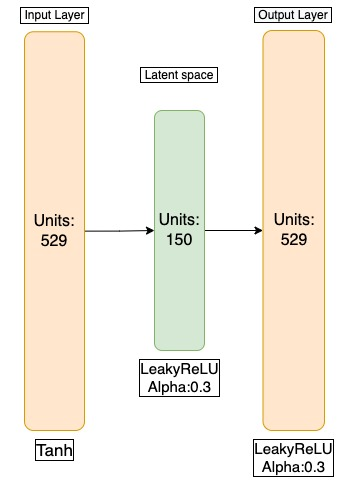
\includegraphics[scale=0.4]{Figures/nnarchitect/ae_small.jpeg}
    \caption[AE | Small network architecture]{Small autoencoder architecture.}
    \label{fig:ae_small}
\end{figure}

In figure \ref{fig:ae_small} we have the small autoencoder. It consists of an input and output layer of 529 nodes, with 
one latent space layer of 150 nodes. The activation functions for the input, latent space and output are the Tanh and 
LeakyReLU with $\alpha=0.3$ respectively, 


\begin{figure}[H]
    \centering
    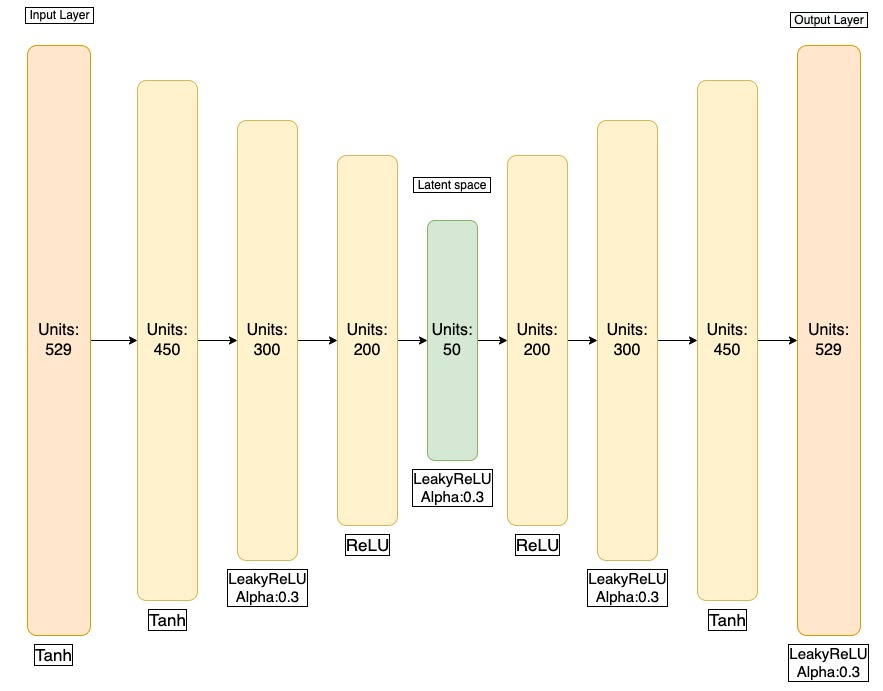
\includegraphics[width=0.8\textwidth]{Figures/nnarchitect/ae_big.jpeg}
    \caption[AE | Large network architecture]{Large autoencoder architecture.}
    \label{fig:ae_big}
\end{figure}

In figure \ref{fig:ae_big} we have the large autoencoder. It consists of an input and output layer of 529 nodes, with three 
hidden layers of 450, 300 and 200 nodes respectively in the encoder and three hidden layers of 200, 300 and 450 respectively. 
The activation functions for the input and ouput layers are the Tanh and LeakyReLU with $\alpha=0.3$ respectively. The hidden 
layers in the encoder have the activation functions Tanh, LeakyReLU with $\alpha=0.3$ and ReLU respectively. The hidden layers
in the decoder have the activation functions ReLU, LeakyReLU with $\alpha=0.3$ and Tanh respectively. The latent space has 150 nodes,
with the LeakyReLU activation function with $\alpha=0.3$.
\subsection*{The variational Autoencoder}
Below are the two models used for the variational autoencoder. 

\begin{figure}[H]
    \centering
    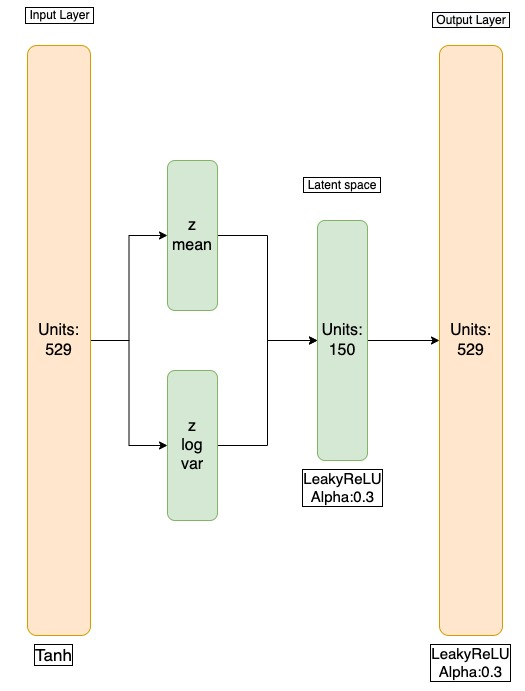
\includegraphics[scale=0.4]{Figures/nnarchitect/vae_small.jpeg}
    \caption[VAE | Small network architecture]{Small variational autoencoder architecture.}
    \label{fig:vae_small}
\end{figure}

In figure \ref{fig:vae_small} we have the small variational autoencoder. It consists of an input and output layer of 529 nodes, with 
one latent space layer of 150 nodes sampling from a mean and variance layer of same size. The activation functions for the input and 
output are the Tanh and LeakyReLU with $\alpha=0.3$ respectively.

\begin{figure}[H]
    \centering
    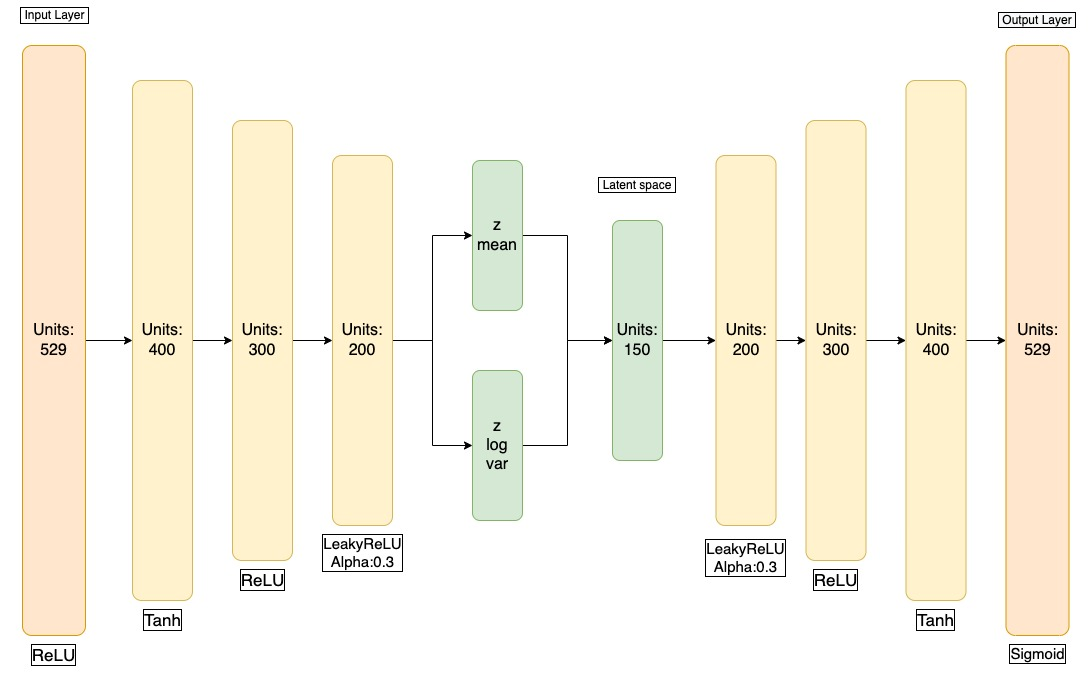
\includegraphics[width=0.8\textwidth]{Figures/nnarchitect/vae_big.jpeg}
    \caption{Large variational autoencoder architecture.}
    \label[VAE | Large network architecture]{fig:vae_big}
\end{figure}


In figure \ref{fig:vae_big} we have the large autoencoder. It consists of an input and output layer of 529 nodes, with three 
hidden layers of 400, 300 and 200 nodes respectively in the encoder and three hidden layers of 200, 300 and 400 respectively. 
The activation functions for the input and ouput layers are the ReLU and Sigmoid respectively. The hidden 
layers in the encoder have the activation functions Tanh, ReLU, LeakyReLU with $\alpha=0.3$ respectively. The hidden layers
in the decoder have the activation functions LeakyReLU with $\alpha=0.3$, ReLU and Tanh respectively.
\section{The search strategy}\label{sec:strategy}
The strategy used to look for anomalies in the 3 lepton + missing energy final state is presented as follows. 
First, the SM MC and ATLAS data for training and inference are constructed with the RMM from section 
\ref{sec:rmm} as features. After scaling and splitting, $80\%$ of the MC will be used for training the neural 
network, and the remaining $20\%$ will be used for inference. The output from the autoencoder will then be used 
to calculate the $log_{10}$ reconstruction error, given as 
\begin{equation}\label{eq:rec_err}
    err = log_{10}\left[ \sum_i (x-\tilde{x})^2\right],
\end{equation}
where $x$ is the input data and $\tilde{x}$ is the autoencoder output. To separate the anomalies, the reconstruction 
error of the input data will create a distribution. The same will then be done for a test signal. The ATLAS data 
is completely unlabeled which makes validation difficult. However, the test signals are labeled, thus we can 
analyze the reconstruction error distribution of those signals as a validation of performance when scientists at 
ATLAS do analysis on ATLAS data. \par
Standard analyses rely on what is called a signal region. The signal region is a region in the feature space in which
the signal is expected to be enriched. These are often not inpected until all analysis selections are fixed ("blind" analysis). 
We use this region to calculate the significance of a result in the search, which is 
really the only metric that is of use. The statistical uncertainty and noise is proportional to the amount of SM MC, 
thus with lower amounts of SM MC, the better the significance will be. Using the reconstruction error, the autoencoder 
can create its own signal region, more specifically the areas of high reconstruction error. A cut here will then be used to 
separate the anomalies from the SM in for example missing transverse energy, or other features of interest. \par 
The signal region for the regular autoencoder models were created by calculating the median $m_{err}$ of the 
reconstruction error. Then, 3 cuts were made, starting at $m_{err} + im_{err}/5$ for $i = 1,2,3$. This was a direct 
result of the shape of the background reconstruction error, being a hill-like shape. The median then became a 
good place to start to remove much of the SM MC. This is however just a guess for an optimal signal region, 
as the true signal is unknown, and the method has to be as unbiased as possible. There is however an issue to keep 
in mind here. The method to find the cut is in some sense based on the slope shape of the SM MC reconstruction 
error distribution, thus three cuts based on the median seems like a good choice. However, if one then uses all 
the events in the signal region, it might be that one misses the ideal amount of background and signal to create 
the significance. Thus, for each reconstruction error cut, there is an associated plot showing the significance 
as a function of $e_T^{miss}$. More specifically, the function calculates from a specific bin and outwards, for all 
bins in the $e_T^{miss}$ distribution. Thus, you can find the ideal cut, within the signal region, for where to 
choose the amount of background and signal to get a better significance.\par 

Since the analysis is based on semi supervised learning, one should avoid tuning on specific signal models.
Therefor one should also prepare a blind test. 
% ROC curves will then be used to evaluate the binary classification ability of the autoencoder. \par 

\section*{Initial testings}
Before testing the AE and VAE on signal samples, it was of interest to test the sensitivity of the
two models on alterings on the Monte Carlo. This can be thought of as initial testing. 
\subsection*{Channel removing}
As the goal of the autoencoder is to reconstruction data is has looked on, one idea was to remove on of the channels in the standard model.
The idea was that some of the channels differs enough in the final states they produce and thus the RMMs for the events in the given selection. 
All channels where tested on as signal, but one can expect some to have more similar results than others. 

\subsection*{Altering transverse momentum}
Another idea for anomaly detection testing with the MonteCarlo was to alter the transverse momentum of some of the particles. Random events where
selected and had the transverse energy changed, in accordance with equation \ref{eq:et}. The hope is that especially events with above 5 time 
increase in transverse momentum should be picked up. Note that by changing the transverse momentum, the change in transverse energy also changes. 
From equation \ref{eq:deltaet} we have that a scale change k in $p_T$ yields the following new relation:

\begin{equation}\label{eq:deltaet_scale}
    \delta\boldsymbol{e_T}^k = \frac{kE_T(i_n-1) - E_T(i_n)}{kE_T(i_n-1) + E_T(i_n)}, \, n = 2, ..., N.
\end{equation}
Thus, both the transverse energy and the change in transverse energy is changed for this test.

\subsection*{Feature shuffling}
Another idea was to shuffle the features of the events. This is done by randomly selecting a feature and swapping it with another feature. 
This will create fake and unphysical events, which should be picked up by the autoencoder. 
\subsection*{Dummy data}
The last idea was to create dummy data. This is done by selecting both a percentage of the rows and columns, and swapping them, 
making the data unphysical. 

%%%%%%%%%%%%%%  Results and Discussion %%%%%%%%%%%%%%%%%%%%%%%
\chapter{Results and Discussion}\label{Chap:results_discuss}
\section{Non signal testing of the regular and variational Autoencoder}




\section{Dummy signal testing of the regular and variational Autoencoder}

Another important part of benchmarking the algorithm is to test it on a signal sample. This is the closest test we can do before
we no longer can alter the algorithm, as that would be supervised learning. Results from both the regular and the variational autoencoder 
are shown below. 

\subsection*{Autoencoder}

\begin{figure}[h!]
    \centering
    \begin{subfigure}{.45\textwidth}
        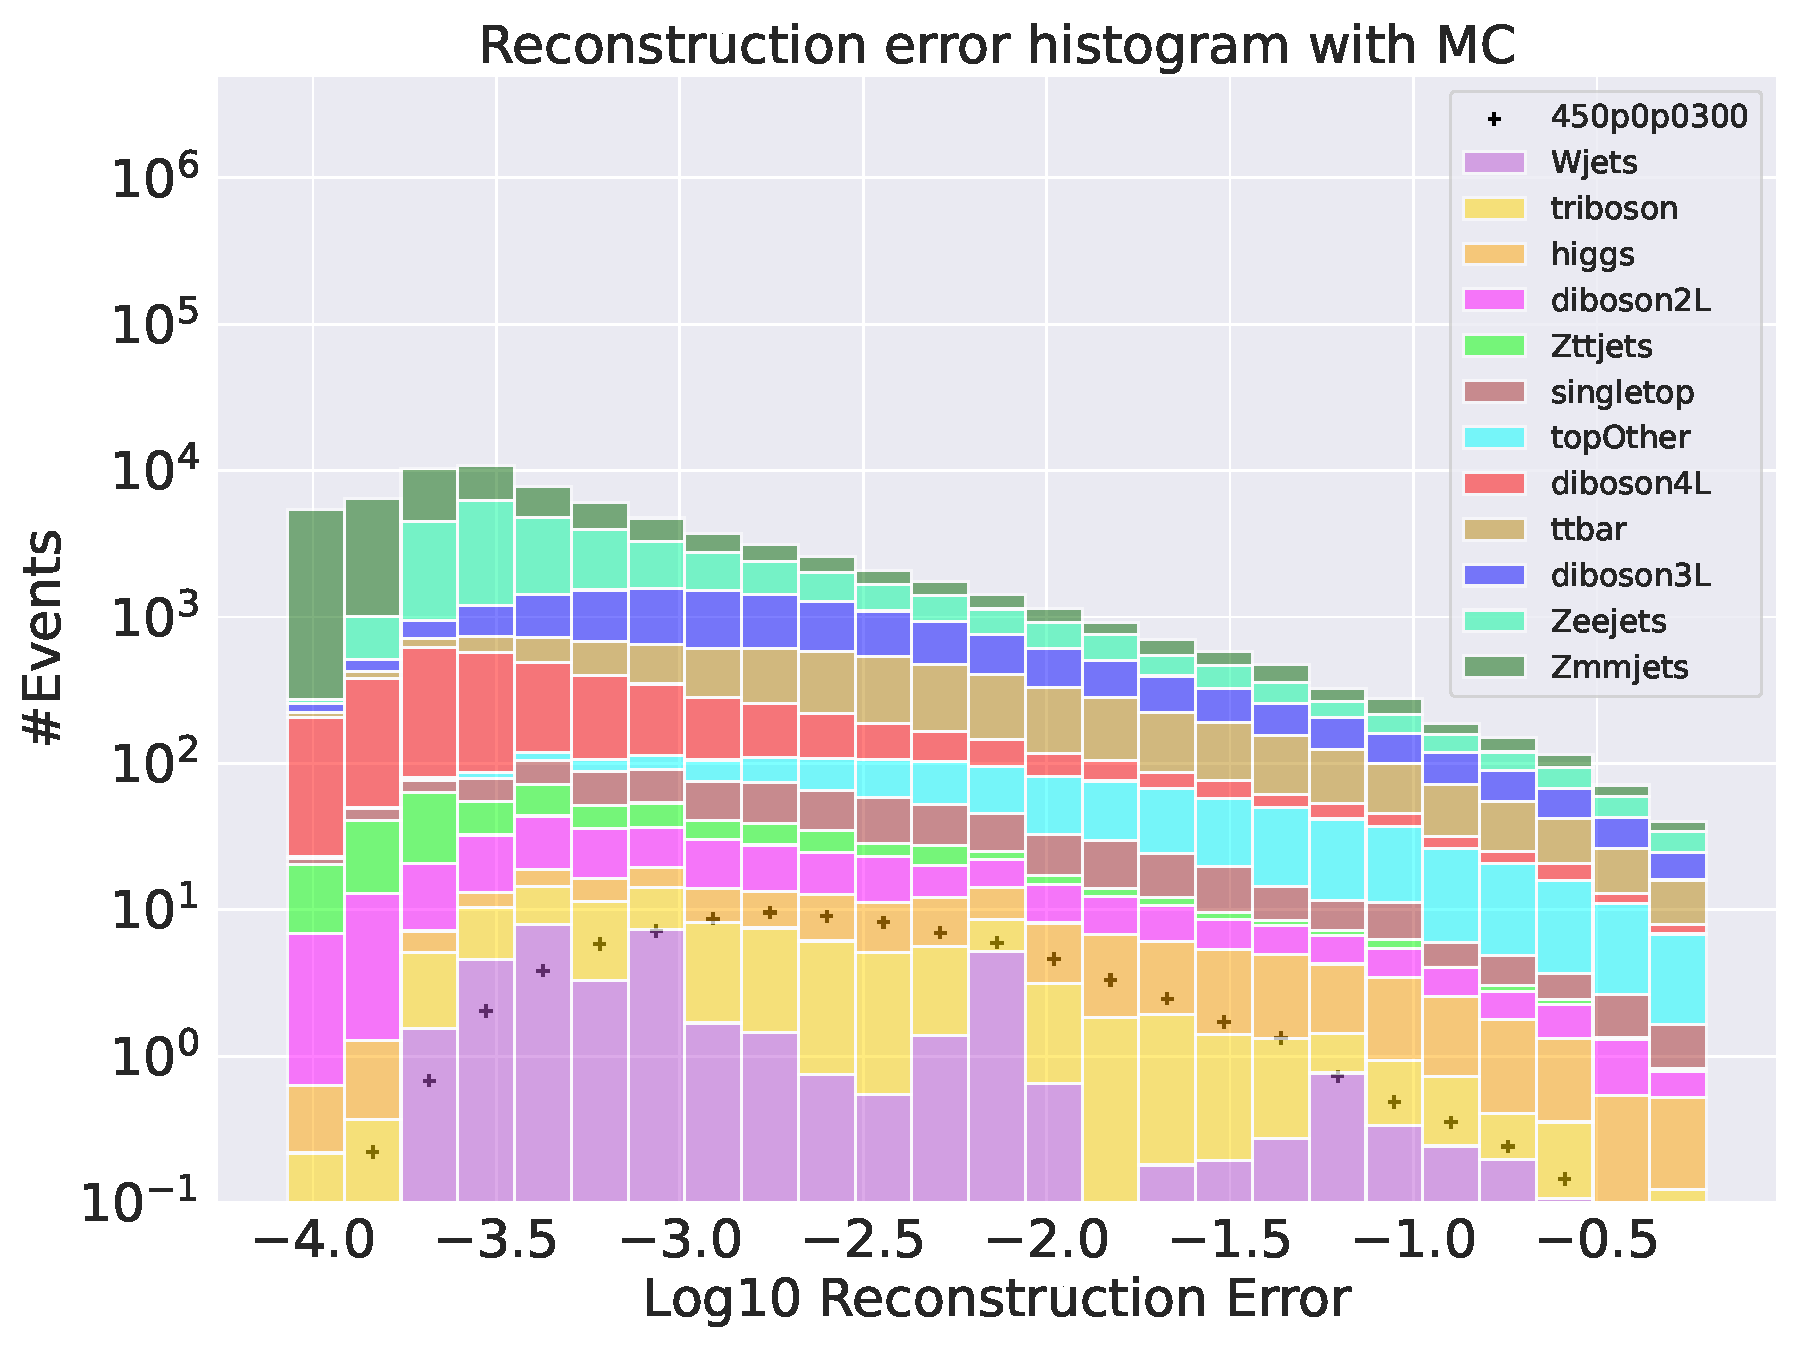
\includegraphics[width=\textwidth]{Figures/AE_testing/small/b_data_recon_big_rm3_feats_sig_450p0p0300.pdf}
        \caption{Reconstruction error on validation SM MC from the Autoencoder. The susy signal is the $450-300$ sample. 
        No significant separation of the distributions are found. }
        \label{fig:ae_susy_450_300_recon}
    \end{subfigure}
    \hfill
    \begin{subfigure}{.45\textwidth}
        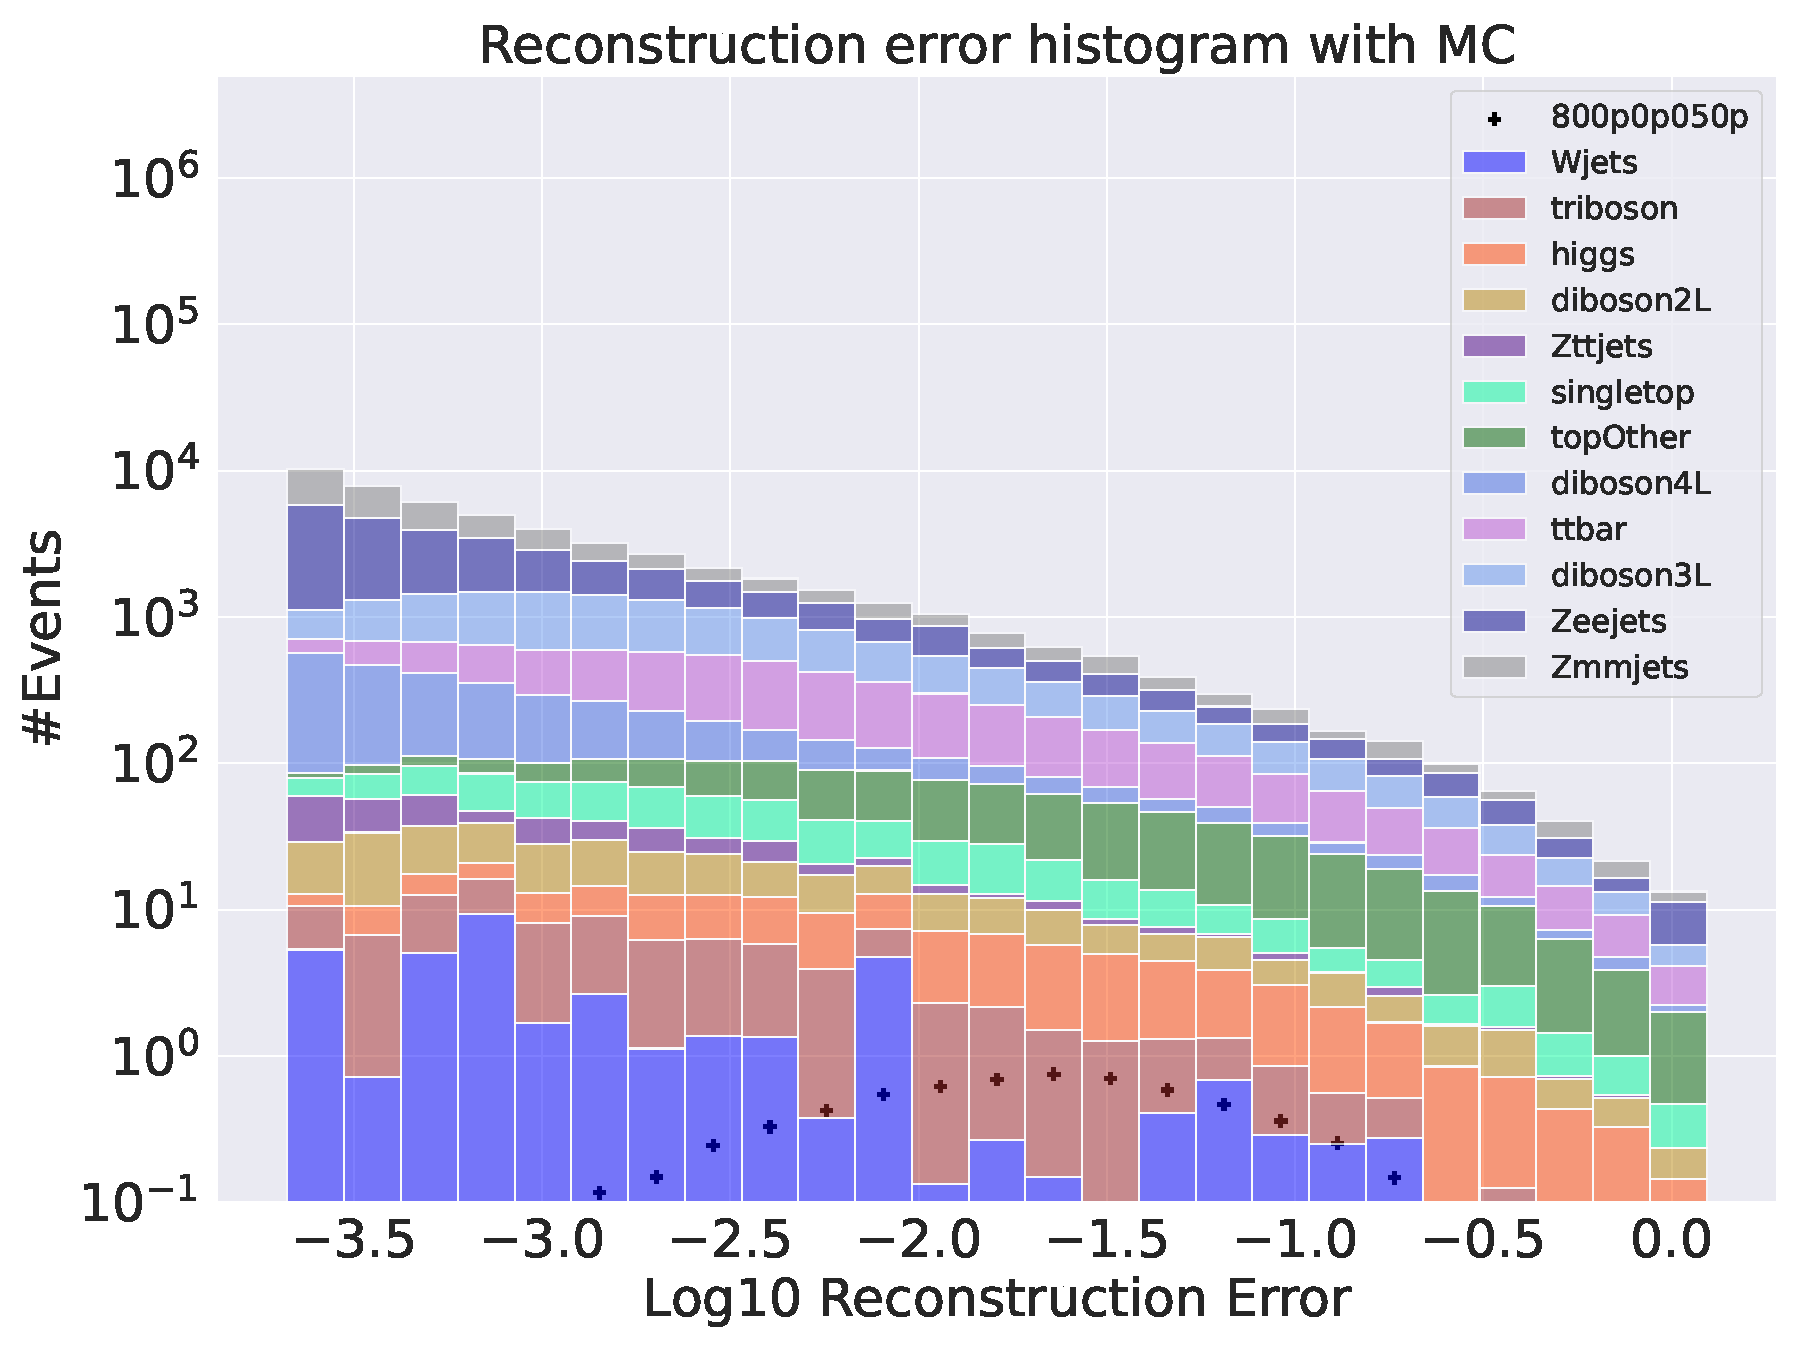
\includegraphics[width=\textwidth]{Figures/AE_testing/small/b_data_recon_big_rm3_feats_sig_800p0p050p.pdf}
        \caption{Reconstruction error on validation SM MC from the Autoencoder. The susy signal is the $800-50$ sample. 
        No significant separation of the distributions are found. }
        \label{fig:ae_susy_800_50_recon}
    \end{subfigure}
    \hfill
    \begin{subfigure}{.45\textwidth}
        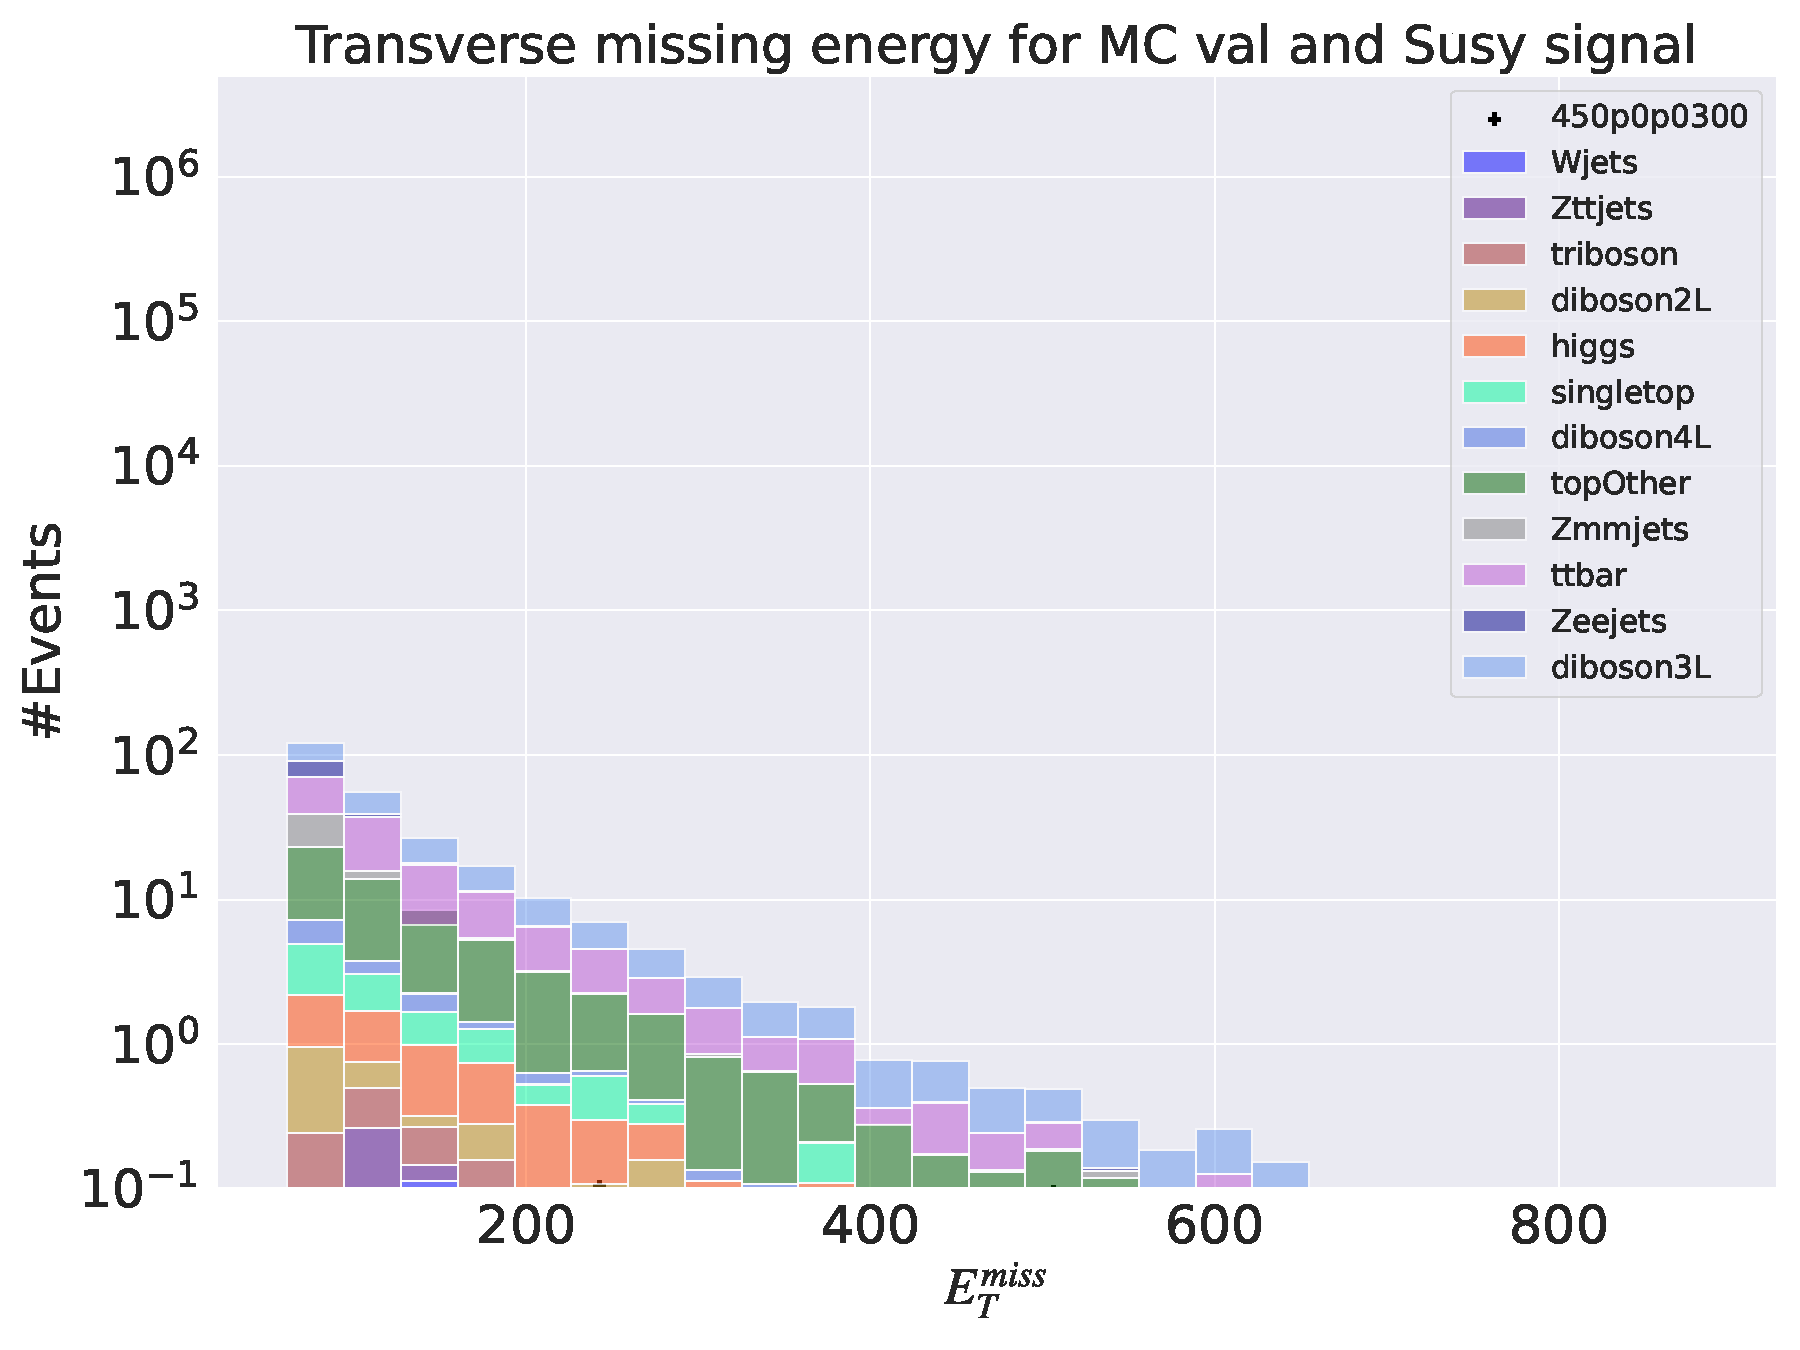
\includegraphics[width=\textwidth]{Figures/AE_testing/small/b_data_recon_big_rm3_feats_sig_450p0p0300_etmiss.pdf}
        \caption{Etmiss bump search for the $450-300$ susy signal. Here events are selected only if reconstruction error is larger than 1. No significant 
        separation of distribution found.}
        \label{fig:ae_susy_450_300_trilep}
    \end{subfigure}
    \hfill        
    \begin{subfigure}{.45\textwidth}
        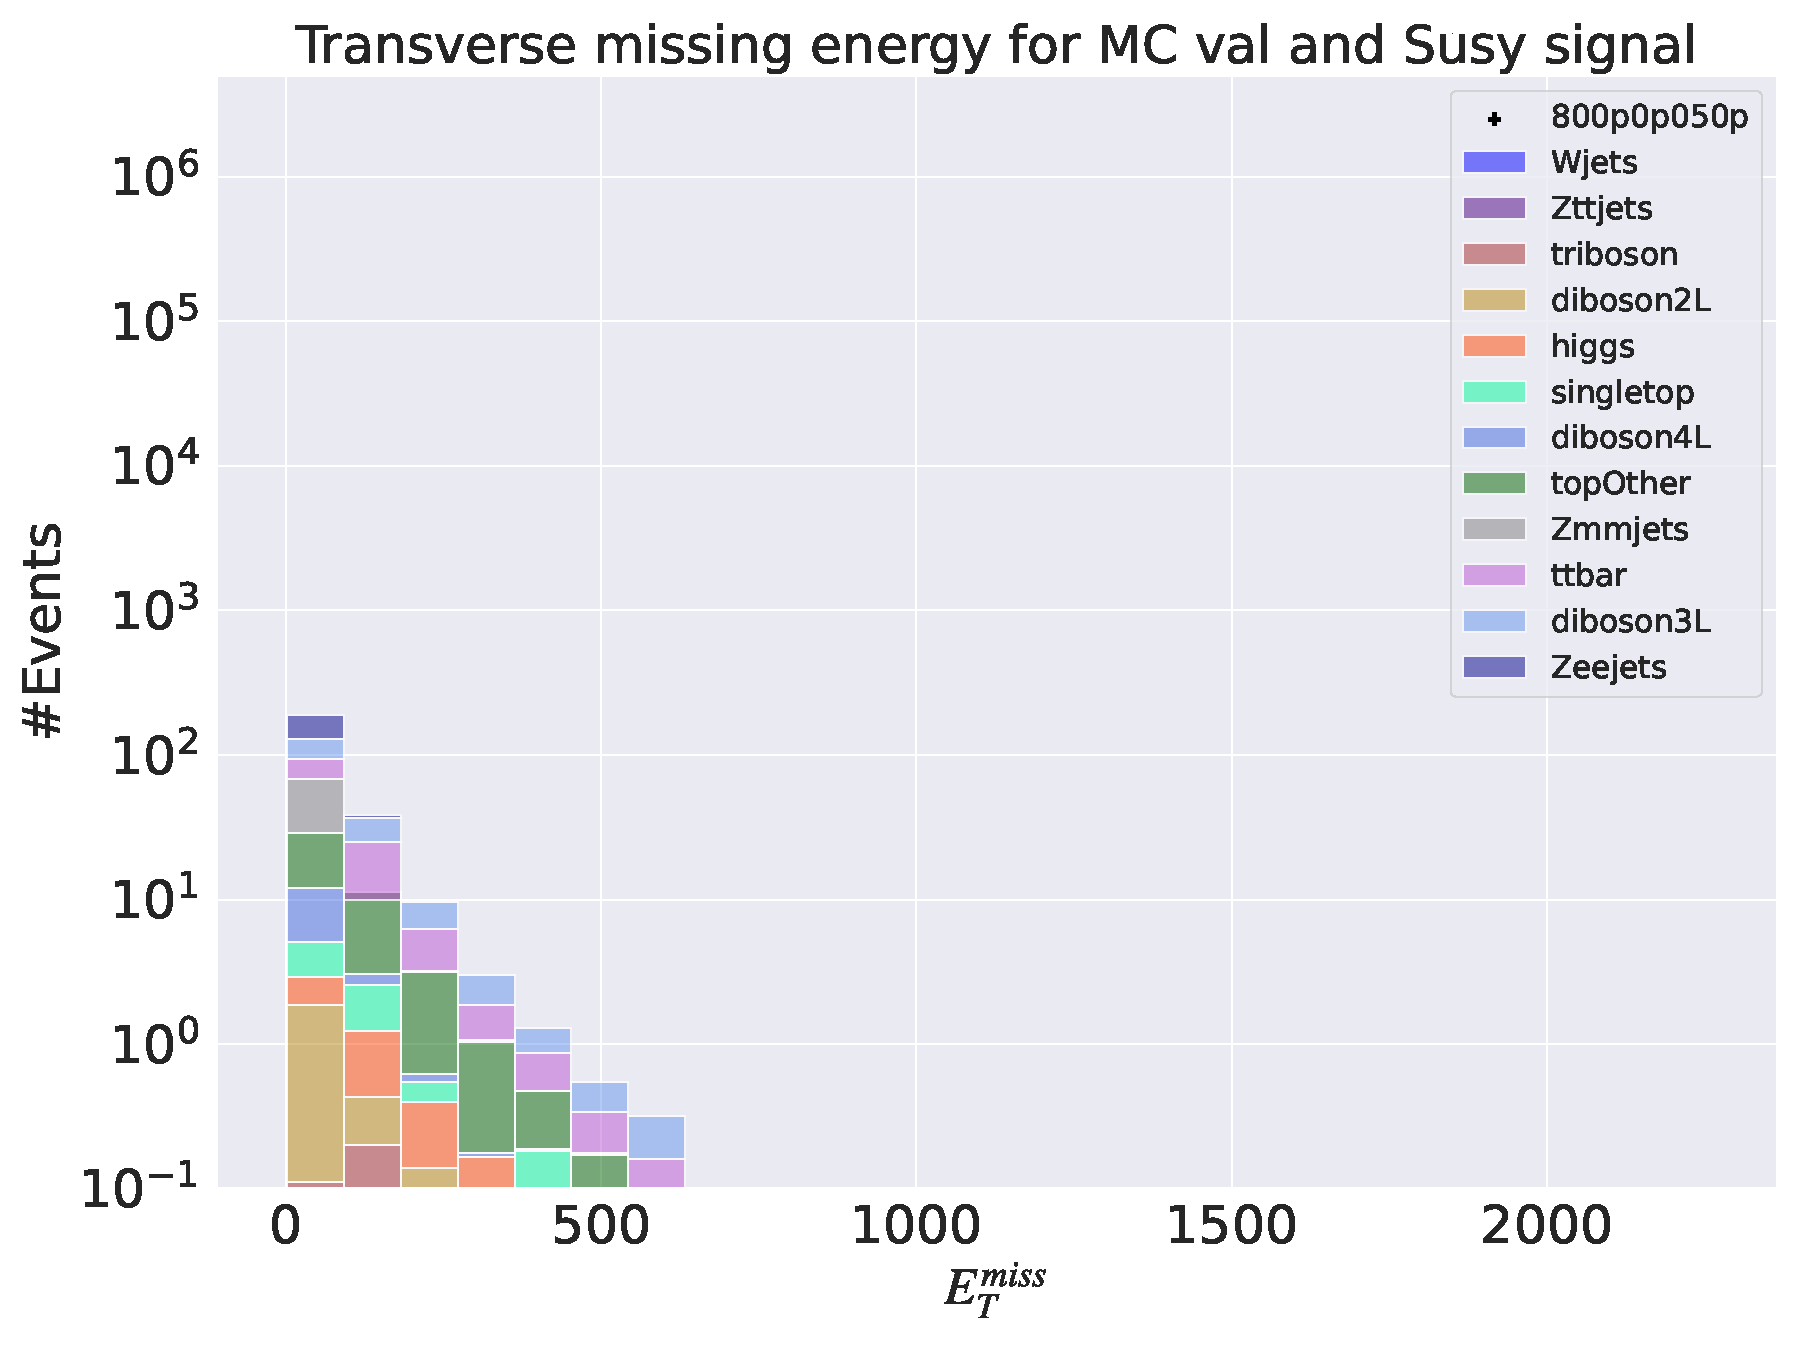
\includegraphics[width=\textwidth]{Figures/AE_testing/small/b_data_recon_big_rm3_feats_sig_800p0p050p_etmiss.pdf}
        \caption{etmiss bump search for the $800-50$ susy signal. Here events are selected only if reconstruction error is larger than 1. No significant 
        separation of distribution found.}
        \label{fig:ae_susy_800_50_trilep}
    \end{subfigure} 
    \hfill     
    \caption{Etmiss bump search on the $450-300$ and $800-50$ susy signals. The reconstruction error cut is set to 1.}
    \label{fig:ae_susy_450_300_800_50_recon_trilep}
\end{figure}


\subsection*{Variational Autoencoder}

\begin{figure}[h!]
    \centering
    \begin{subfigure}{.45\textwidth}
        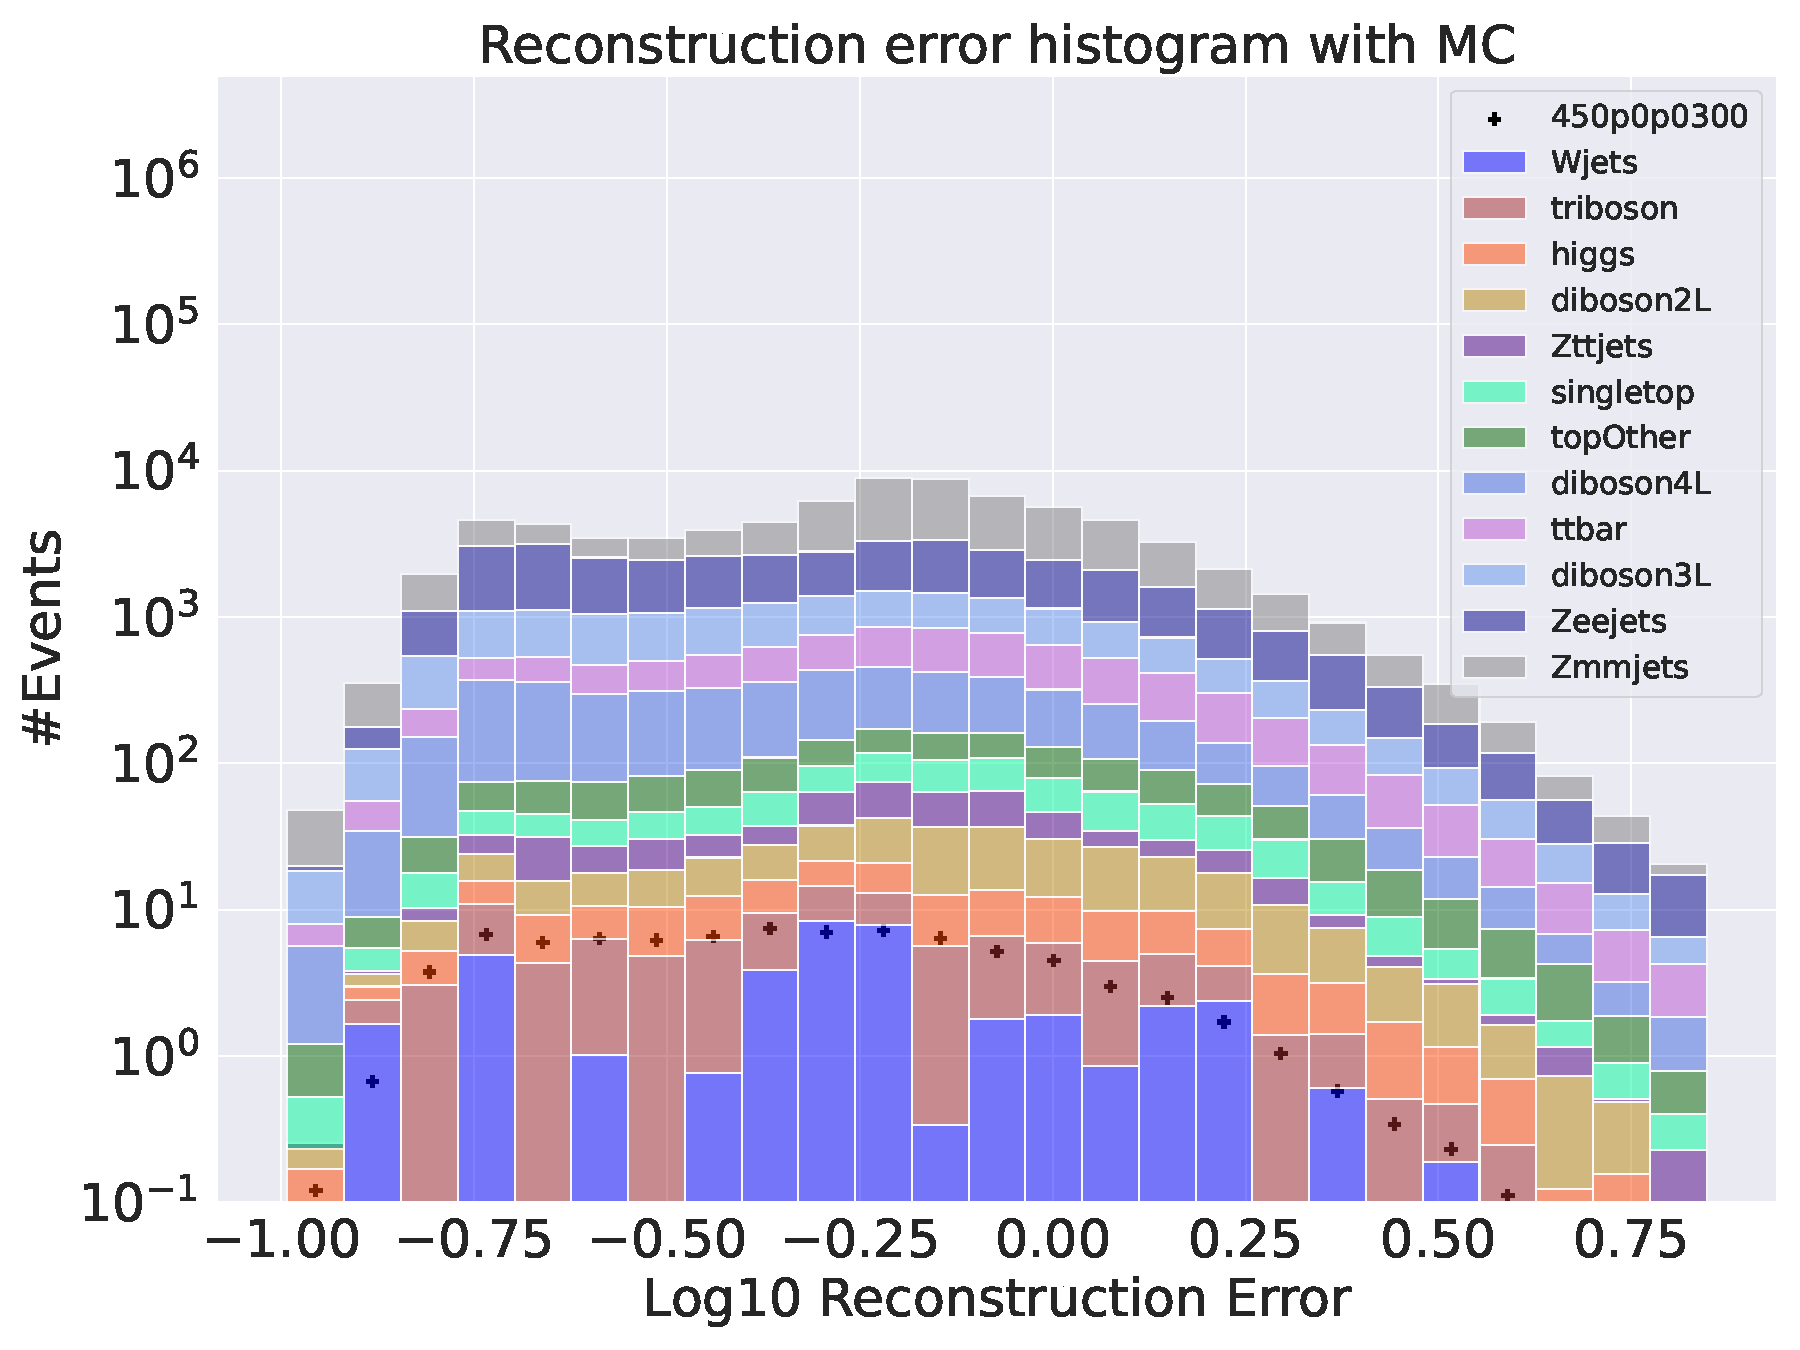
\includegraphics[width=\textwidth]{Figures/VAE_testing/small/b_data_recon_big_rm3_feats_sig_450p0p0300.pdf}
        \caption{Reconstruction error on validation SM MC from the variational Autoencoder. The susy signal is the $450-300$ sample. 
        No significant separation of the distributions are found. }
        \label{fig:vae_susy_450_300_recon}
    \end{subfigure}
    \hfill
    \begin{subfigure}{.45\textwidth}
        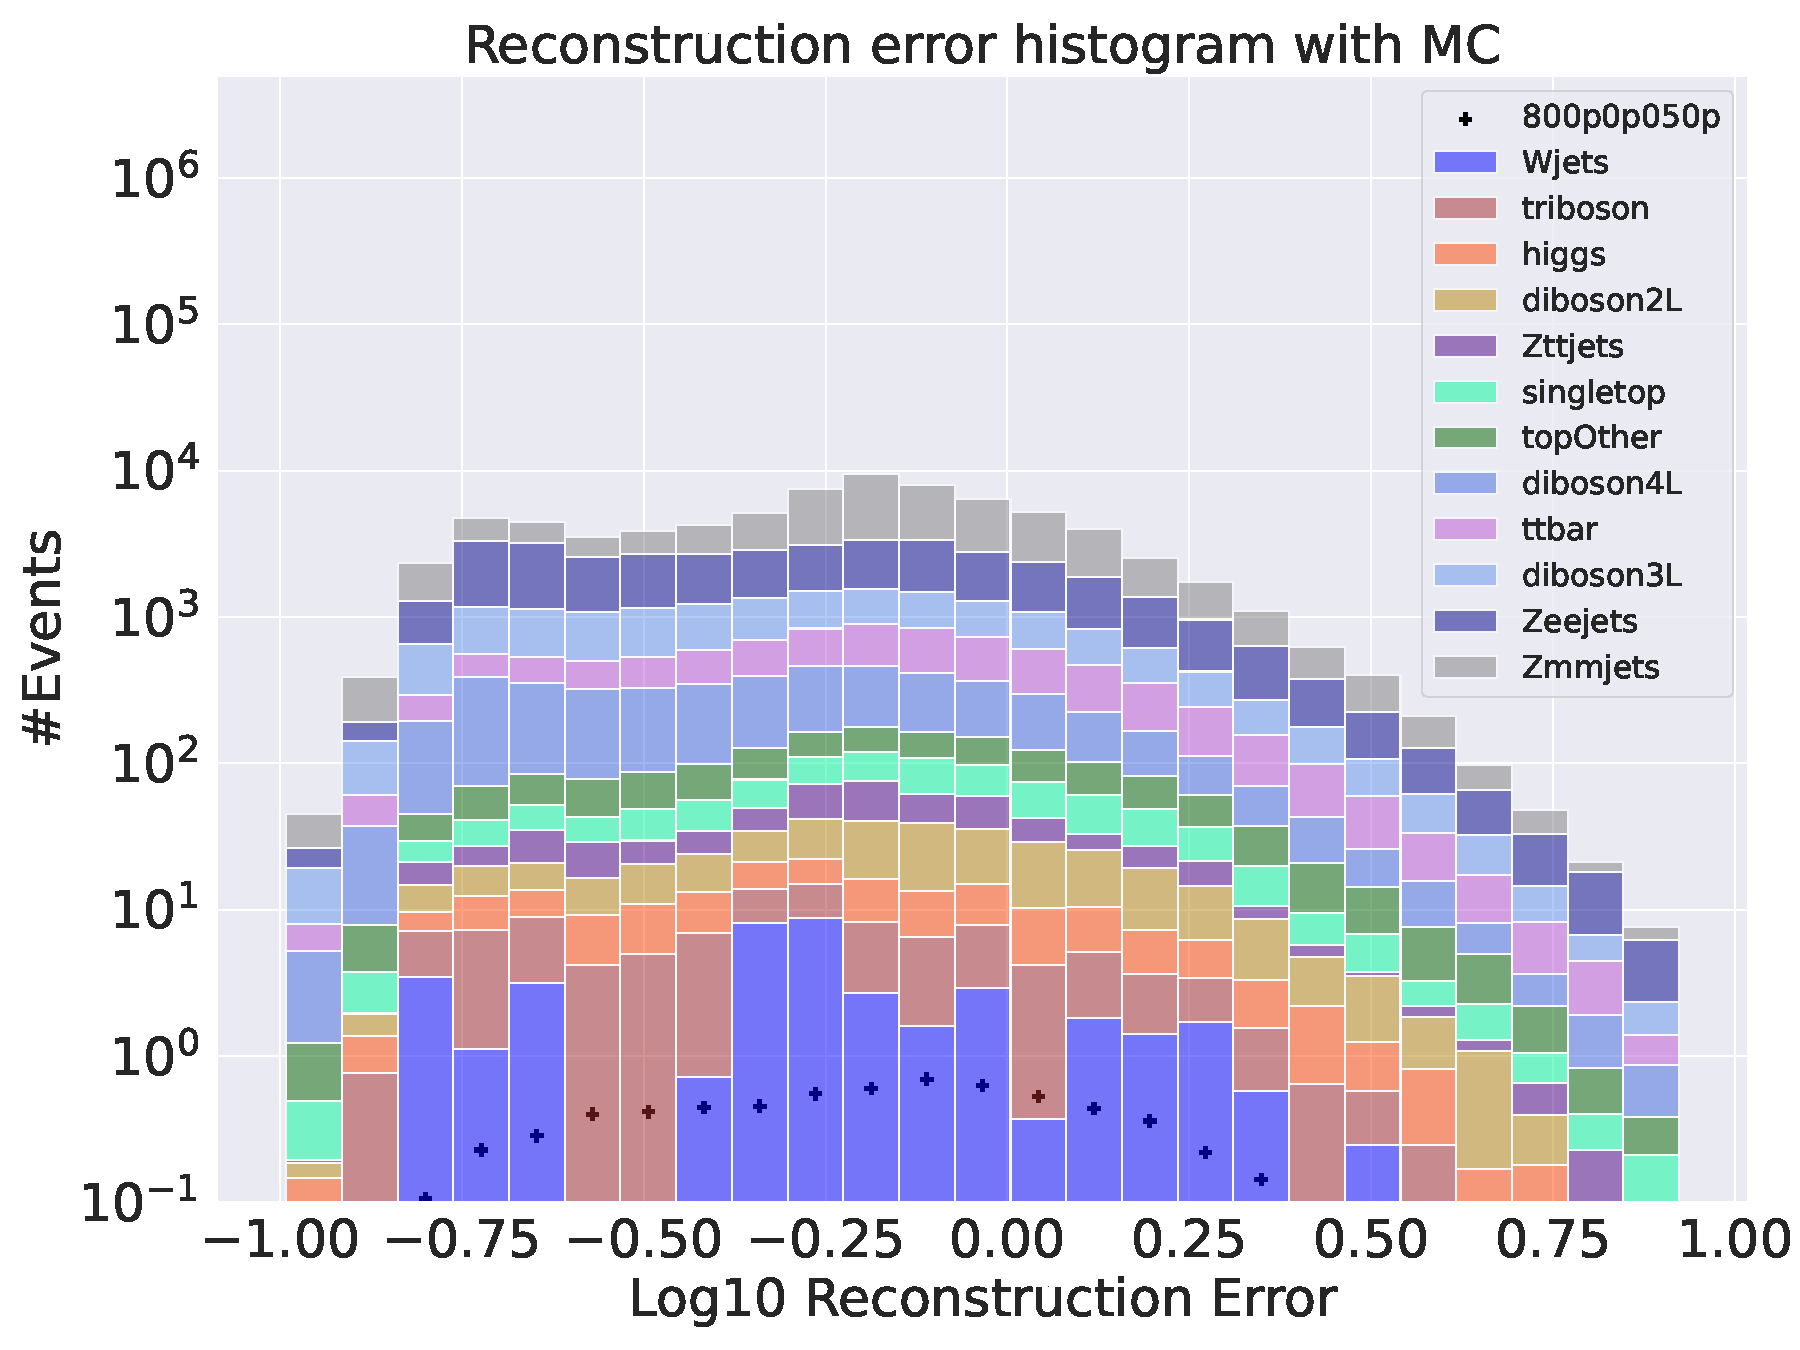
\includegraphics[width=\textwidth]{Figures/VAE_testing/small/b_data_recon_big_rm3_feats_sig_800p0p050p.pdf}
        \caption{Reconstruction error on validation SM MC from the variational Autoencoder. The susy signal is the $800-50$ sample. 
        No significant separation of the distributions are found. }
        \label{fig:vae_susy_800_50_recon}
    \end{subfigure}
    \hfill
    \begin{subfigure}{.45\textwidth}
        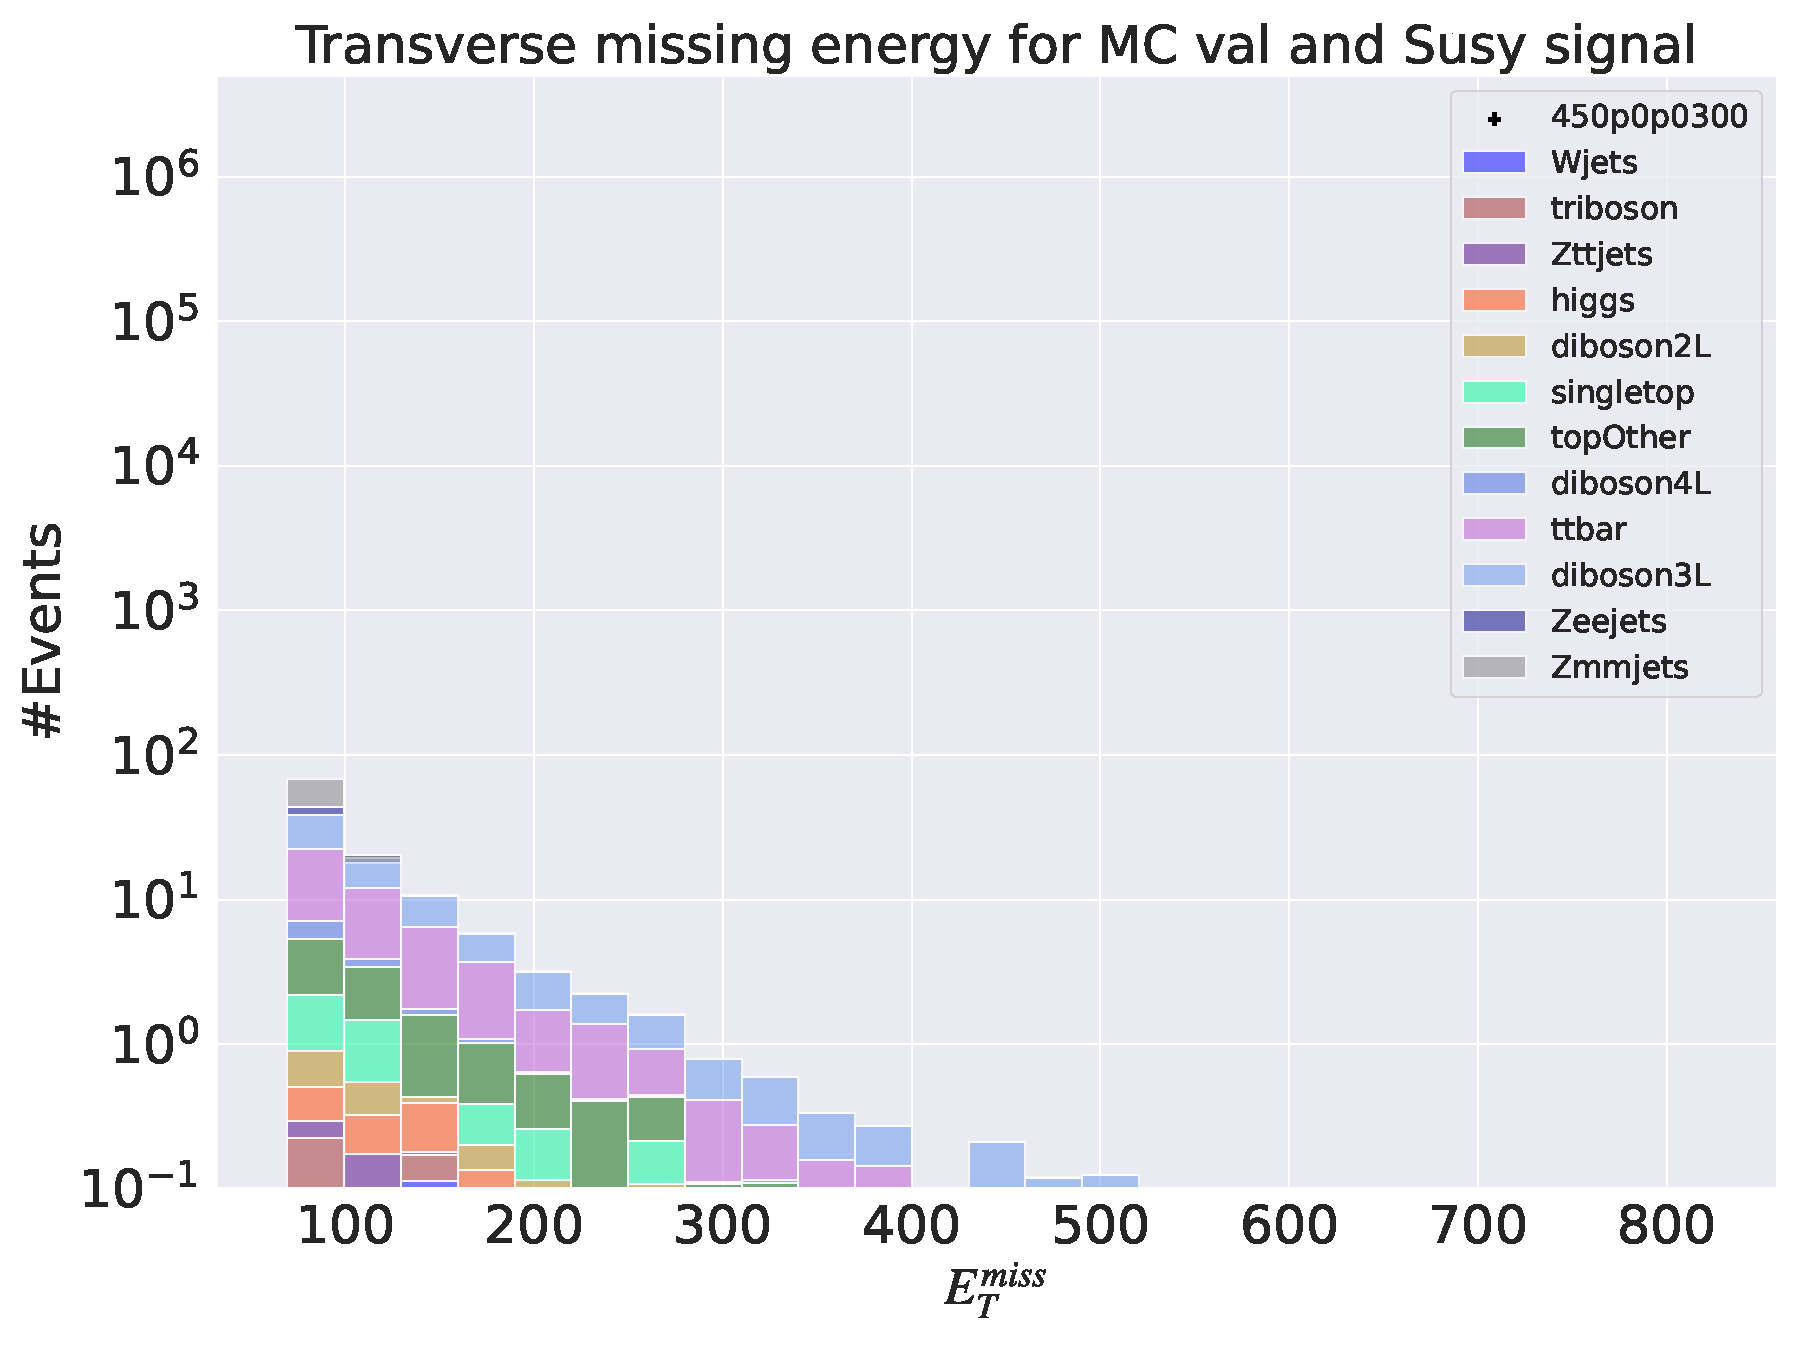
\includegraphics[width=\textwidth]{Figures/VAE_testing/small/b_data_recon_big_rm3_feats_sig_450p0p0300_etmiss.pdf}
        \caption{etmiss bump search for the $450-300$ susy signal. Here events are selected only if reconstruction error is larger than 1. No significant 
        separation of distribution found.}
        \label{fig:vae_susy_450_300_trilep}
    \end{subfigure}
    \hfill   
    \begin{subfigure}{.45\textwidth}
        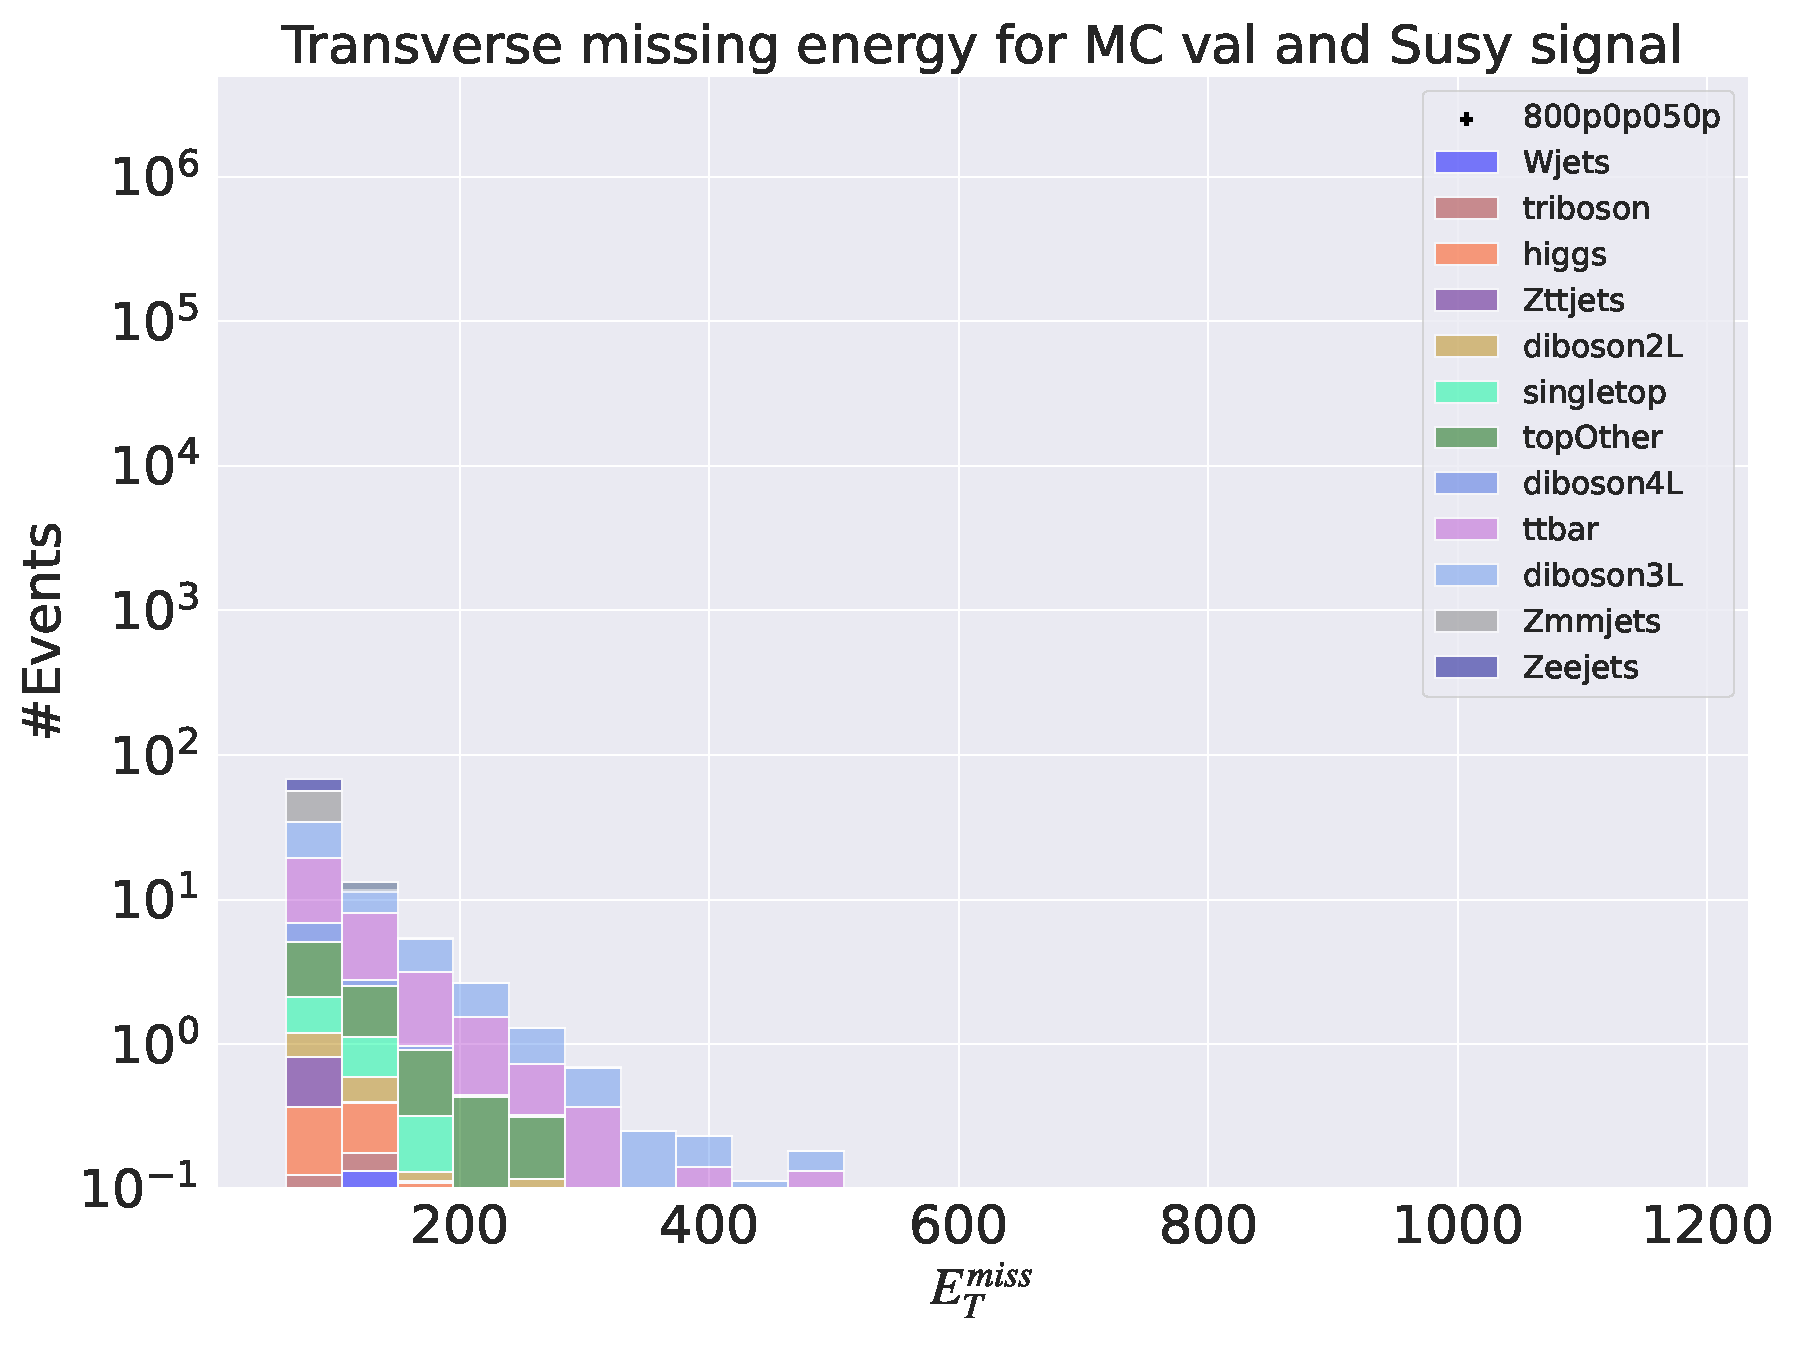
\includegraphics[width=\textwidth]{Figures/VAE_testing/small/b_data_recon_big_rm3_feats_sig_800p0p050p_etmiss.pdf}
        \caption{etmiss bump search for the $800-50$ susy signal. Here events are selected only if reconstruction error is larger than 1. No significant 
        separation of distribution found.}
        \label{fig:vae_susy_800_50_trilep}
    \end{subfigure}
    \hfill      
    \caption{ Reconstruction error and etmiss bump search on the $450-300$ and $800-50$ susy signals. The reconstruction error cut is set to 1.}
    \label{fig:vae_susy_450_300_800_50_recon_trilep}
\end{figure}


\newpage
\subsection*{ROC curves on $e_T^{miss}$ and reconstruction error}
Now based on the reconstruction error on the SUSY signals, especially the one in figure \ref{fig:ae_susy_800_50_recon}, it is tempting to declare that the autoencoder 
has done a good job reconstructing the standard model and a poor job on the SUSY signal, resulting in a separation of distributions. However, there is one thing we need to remember. 
The SUSY signals have very high $e_T^{miss}$, so much so that one can separate them by eye on that distribution alone. This is presented in the figure below:

\begin{figure}[h!]
    \centering
    \begin{subfigure}{.45\textwidth}
    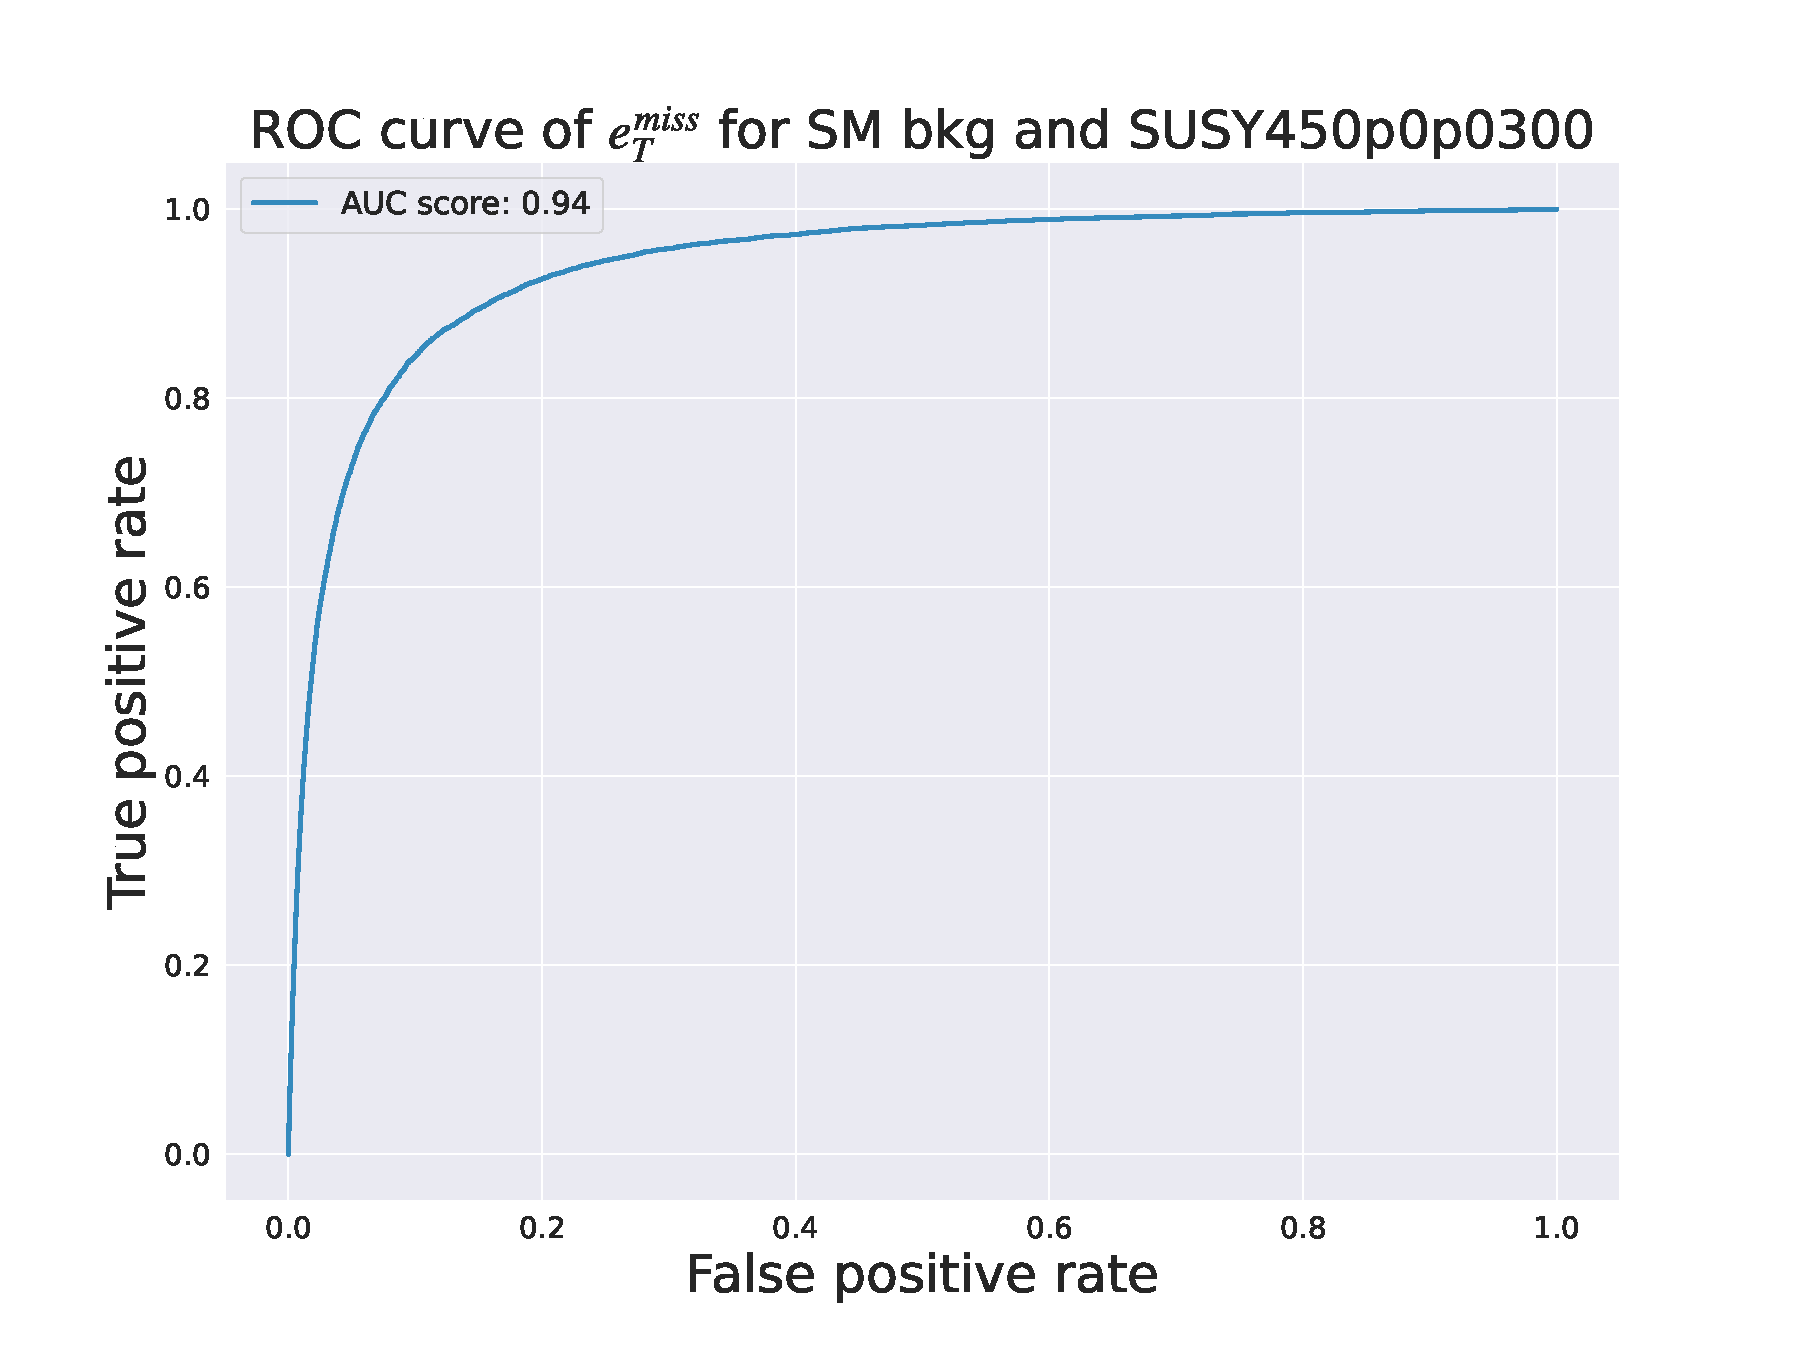
\includegraphics[width=\textwidth]{Figures/AE_testing/big/roc_curve_etmiss_450p0p0300.pdf}
        \caption{ROC curve for $e_T^{miss}$ of both SM MC and the SUSY $450-300$ signal. We see here that based on that feature alone, you can separate 
        the distributions with reative ease, with an AUC of about 0.94. }
    \end{subfigure}
    \hfill
    \begin{subfigure}{.45\textwidth}
        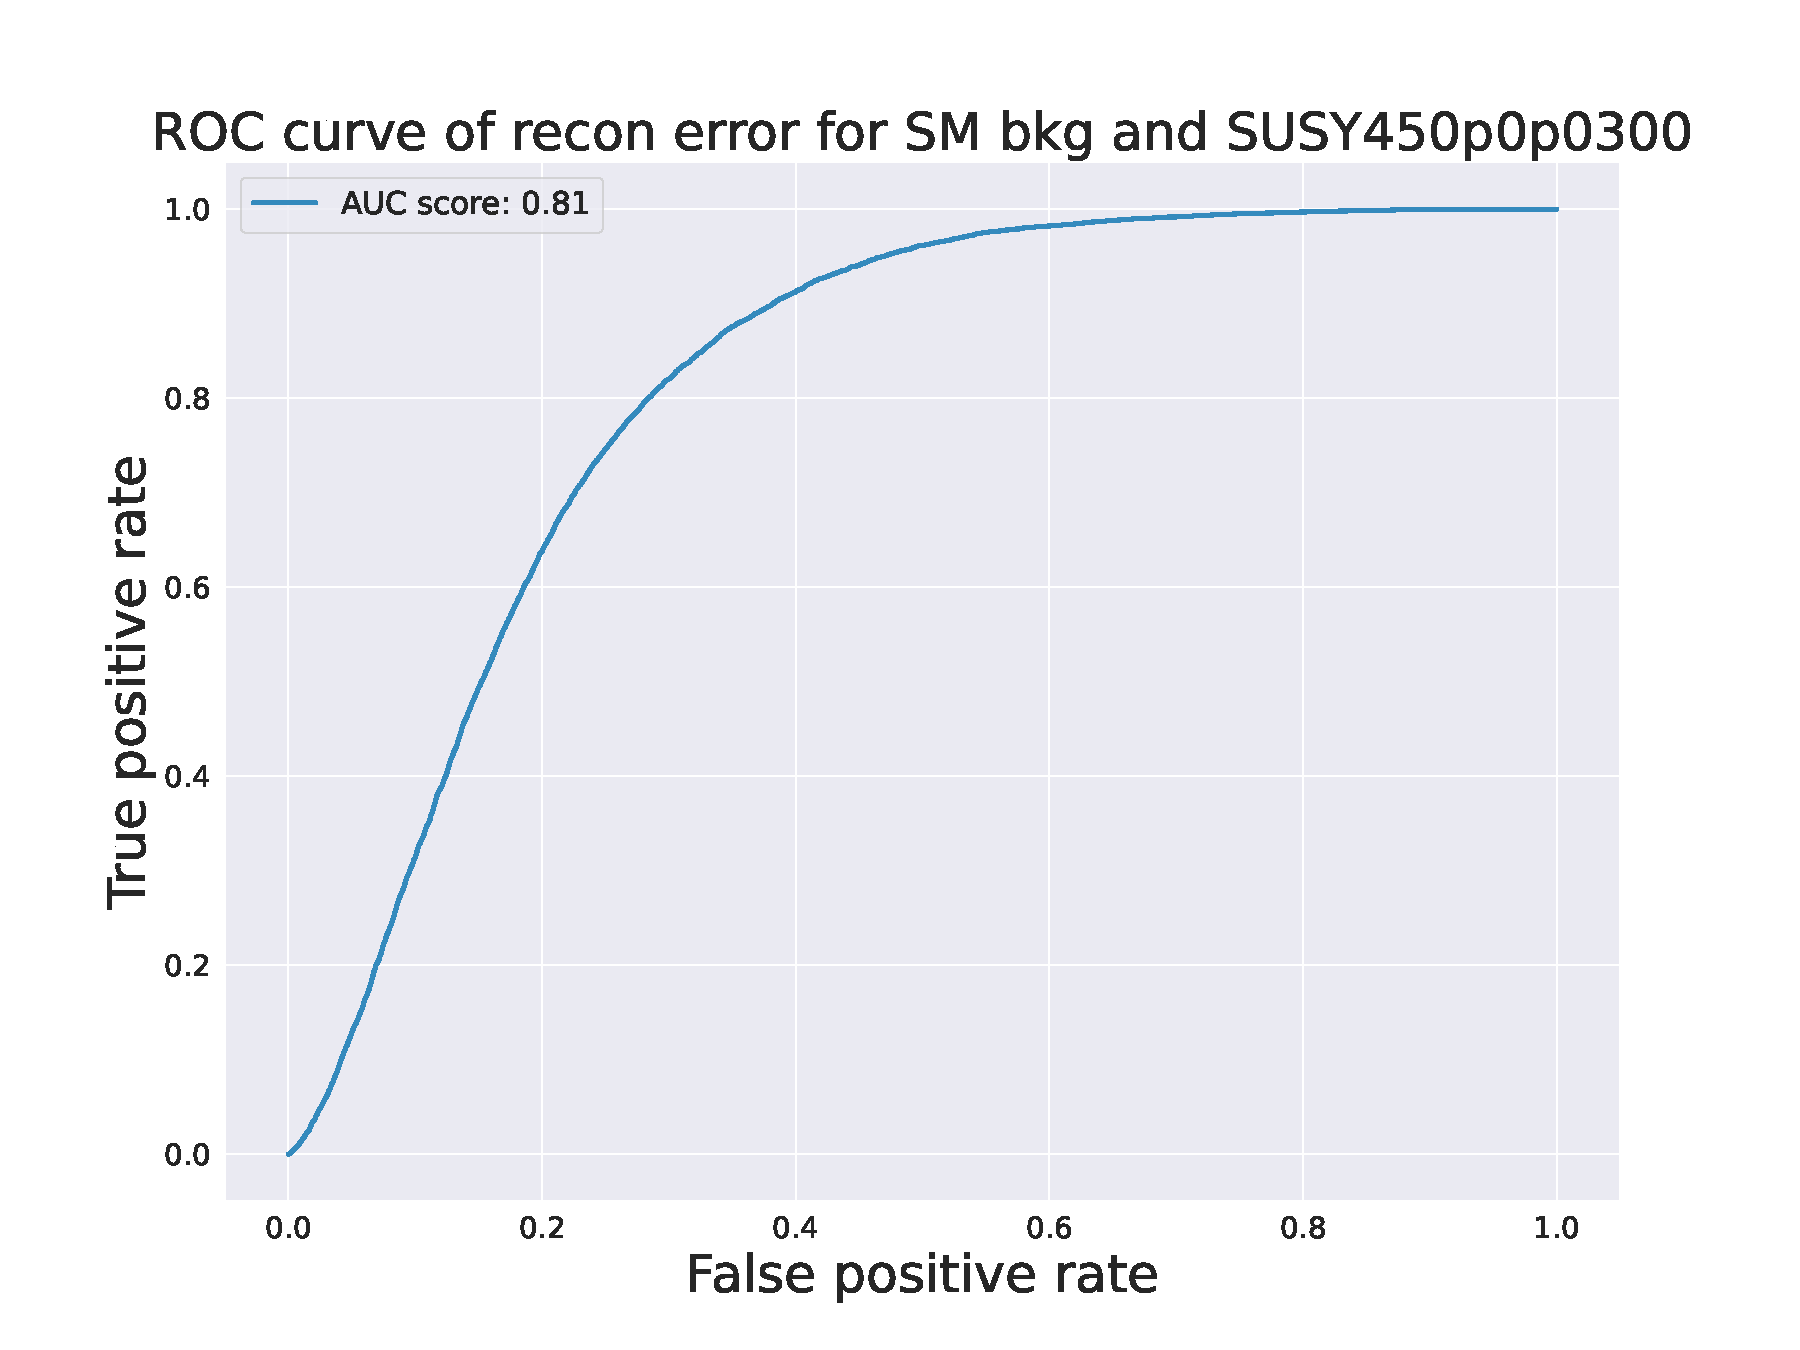
\includegraphics[width=\textwidth]{Figures/AE_testing/big/roc_curve_recon_err_450p0p0300.pdf}
            \caption{ROC curve for reconstruction error of both SM MC and the SUSY $450-300$ signal. We see here that there is relatively good separation,
            with a small AUC of about 0.81.}
        \end{subfigure}
        \hfill
    \caption{ROC curve for both $e_T^{miss}$ and reconstruction error with the SUSY $450-300$ signal. }
    \label{fig:roc_susy_450_300}
\end{figure}



\begin{figure}[h!]
    \centering
    \begin{subfigure}{.45\textwidth}
    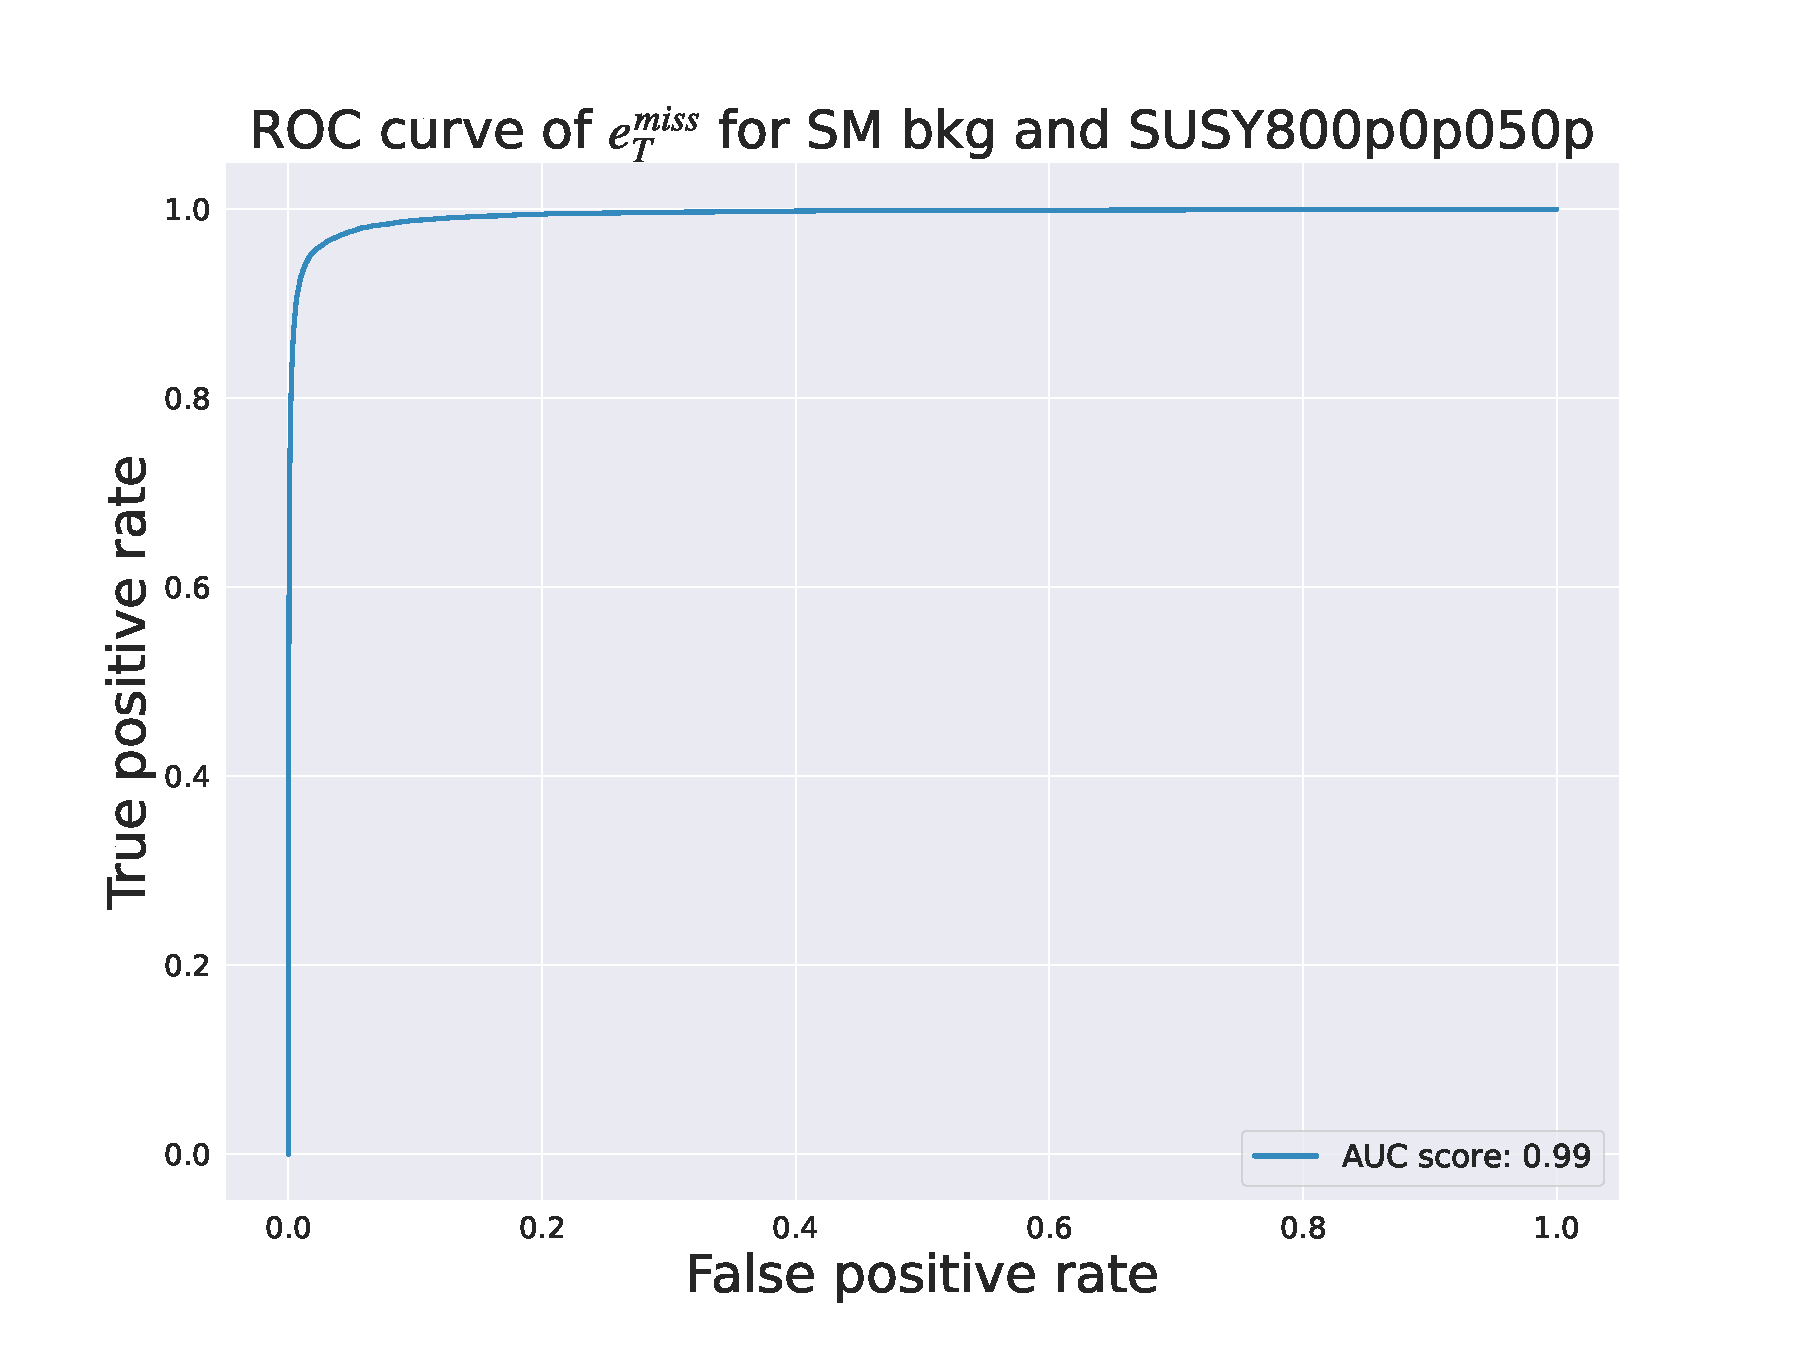
\includegraphics[width=\textwidth]{Figures/AE_testing/big/roc_curve_etmiss_800p0p050p.pdf}
        \caption{ROC curve for $e_T^{miss}$ of both SM MC and the SUSY $800-50$ signal. We see here that based on that feature alone, you can separate 
        the distributions with reative ease, with an AUC of about 0.99. }
    \end{subfigure}
    \hfill
    \begin{subfigure}{.45\textwidth}
        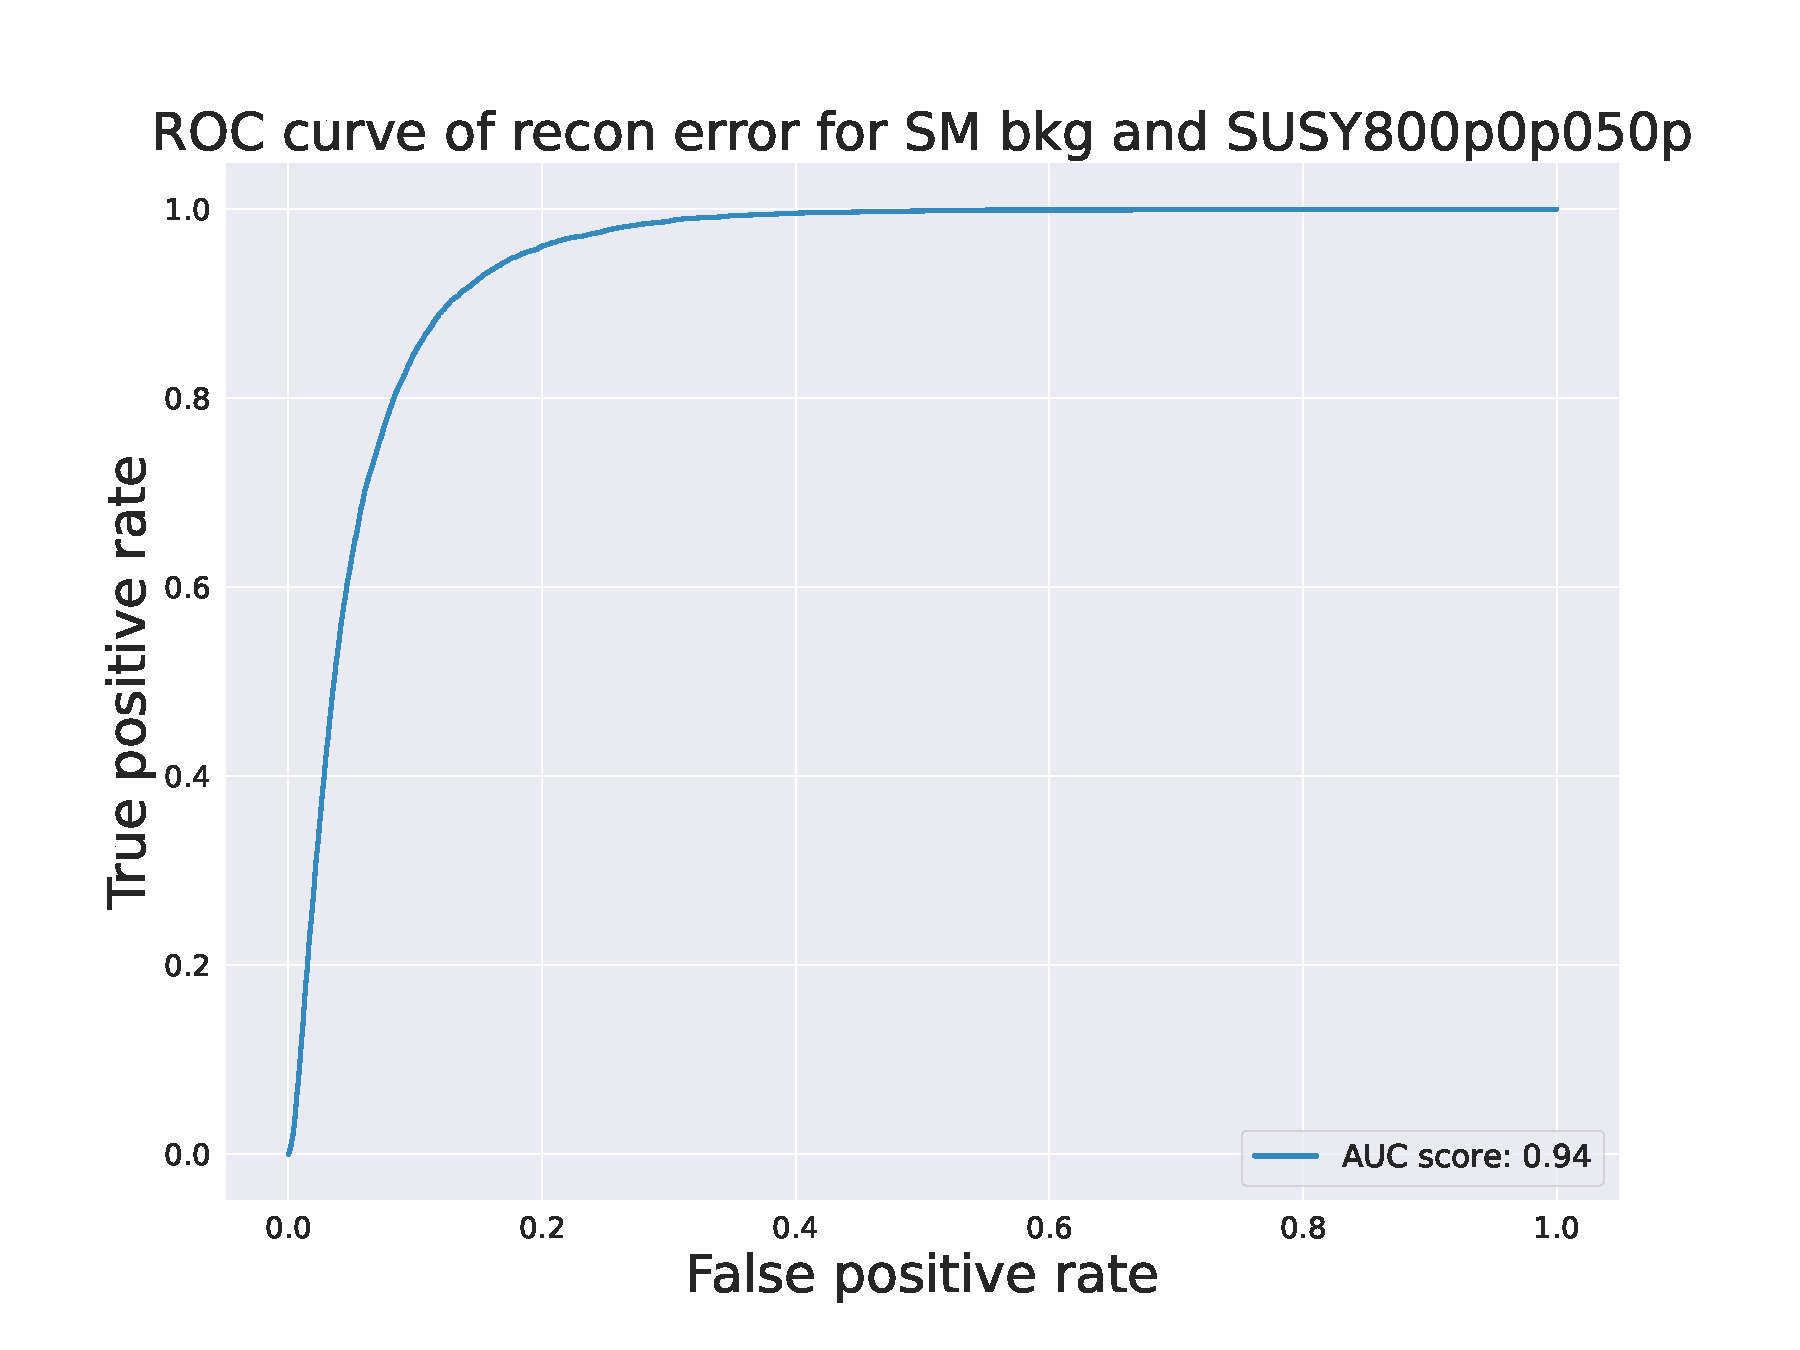
\includegraphics[width=\textwidth]{Figures/AE_testing/big/roc_curve_recon_err_800p0p050p.pdf}
            \caption{ROC curve for reconstruction error of both SM MC and the SUSY $800-50$ signal. We see here that there is a very good separation between the distributions
            , with an AUC of about 0.94.}
        \end{subfigure}
        \hfill
    \caption{ }
    \label{fig:roc_susy_800_50}
\end{figure}

From figure \ref{fig:roc_susy_450_300} and \ref{fig:roc_susy_800_50} we see that even though the reconstruction error is a good discriminator for the SM MC and the SUSY signals, 
$e_T^{miss}$ provides better separation. This is because the SUSY signals have very high $e_T^{miss}$, so much so that one can separate them by eye on that distribution alone. 
The interpretation of this is that the autoencoder has shown it can be used for the purpose of separating the SM MC from the SUSY signals, but not to the level of using just $e_T^{miss}$. 
The same behavior is shown for the small autoencoder in the appendix, aswell as for the small and large variational autoencoder. 
\section{3 lepton ATLAS data analysis}

\subsection*{Heavy neutrino signal testing of the regular and variational Autoencoder}

\section{2 lepton training for bump search testing}\label{sec:2lep}

The 3 lepton + $e_T^{miss}$ dataset has fewer events, and thus allows for less training of the neural networks. 
Thus, the 2 lepton + $e_T^{miss}$ dataset was tried as well. The event selection was done choosing at least 
2 leptons, meaning that the RMM signatures of some events will look similar to the RMM signatures of 
the 3 lepton + $e_T^{miss}$ dataset. A consequence of this is that the signal samples for the 3 lepton case 
will be a good start point for testing. The two autoencoders will be tested on three of the 
four metrics used for the 3 lepton + $e_T^{miss}$ case. 
\begin{itemize}
    \item Low reconstruction error on SM MC
    \item Background to signal ratio in $e_T^{miss}$ signal region
    \item Significance search in $e_T^{miss}$ signal region
\end{itemize}

\subsubsection*{Regular autoencoder performance}
Below are some results from training on the 2 lepton case with the regular autoencoder, using the same two SUSY signals as test cases. 

\begin{figure}[H]
    \centering
    \begin{subfigure}{.45\textwidth}
        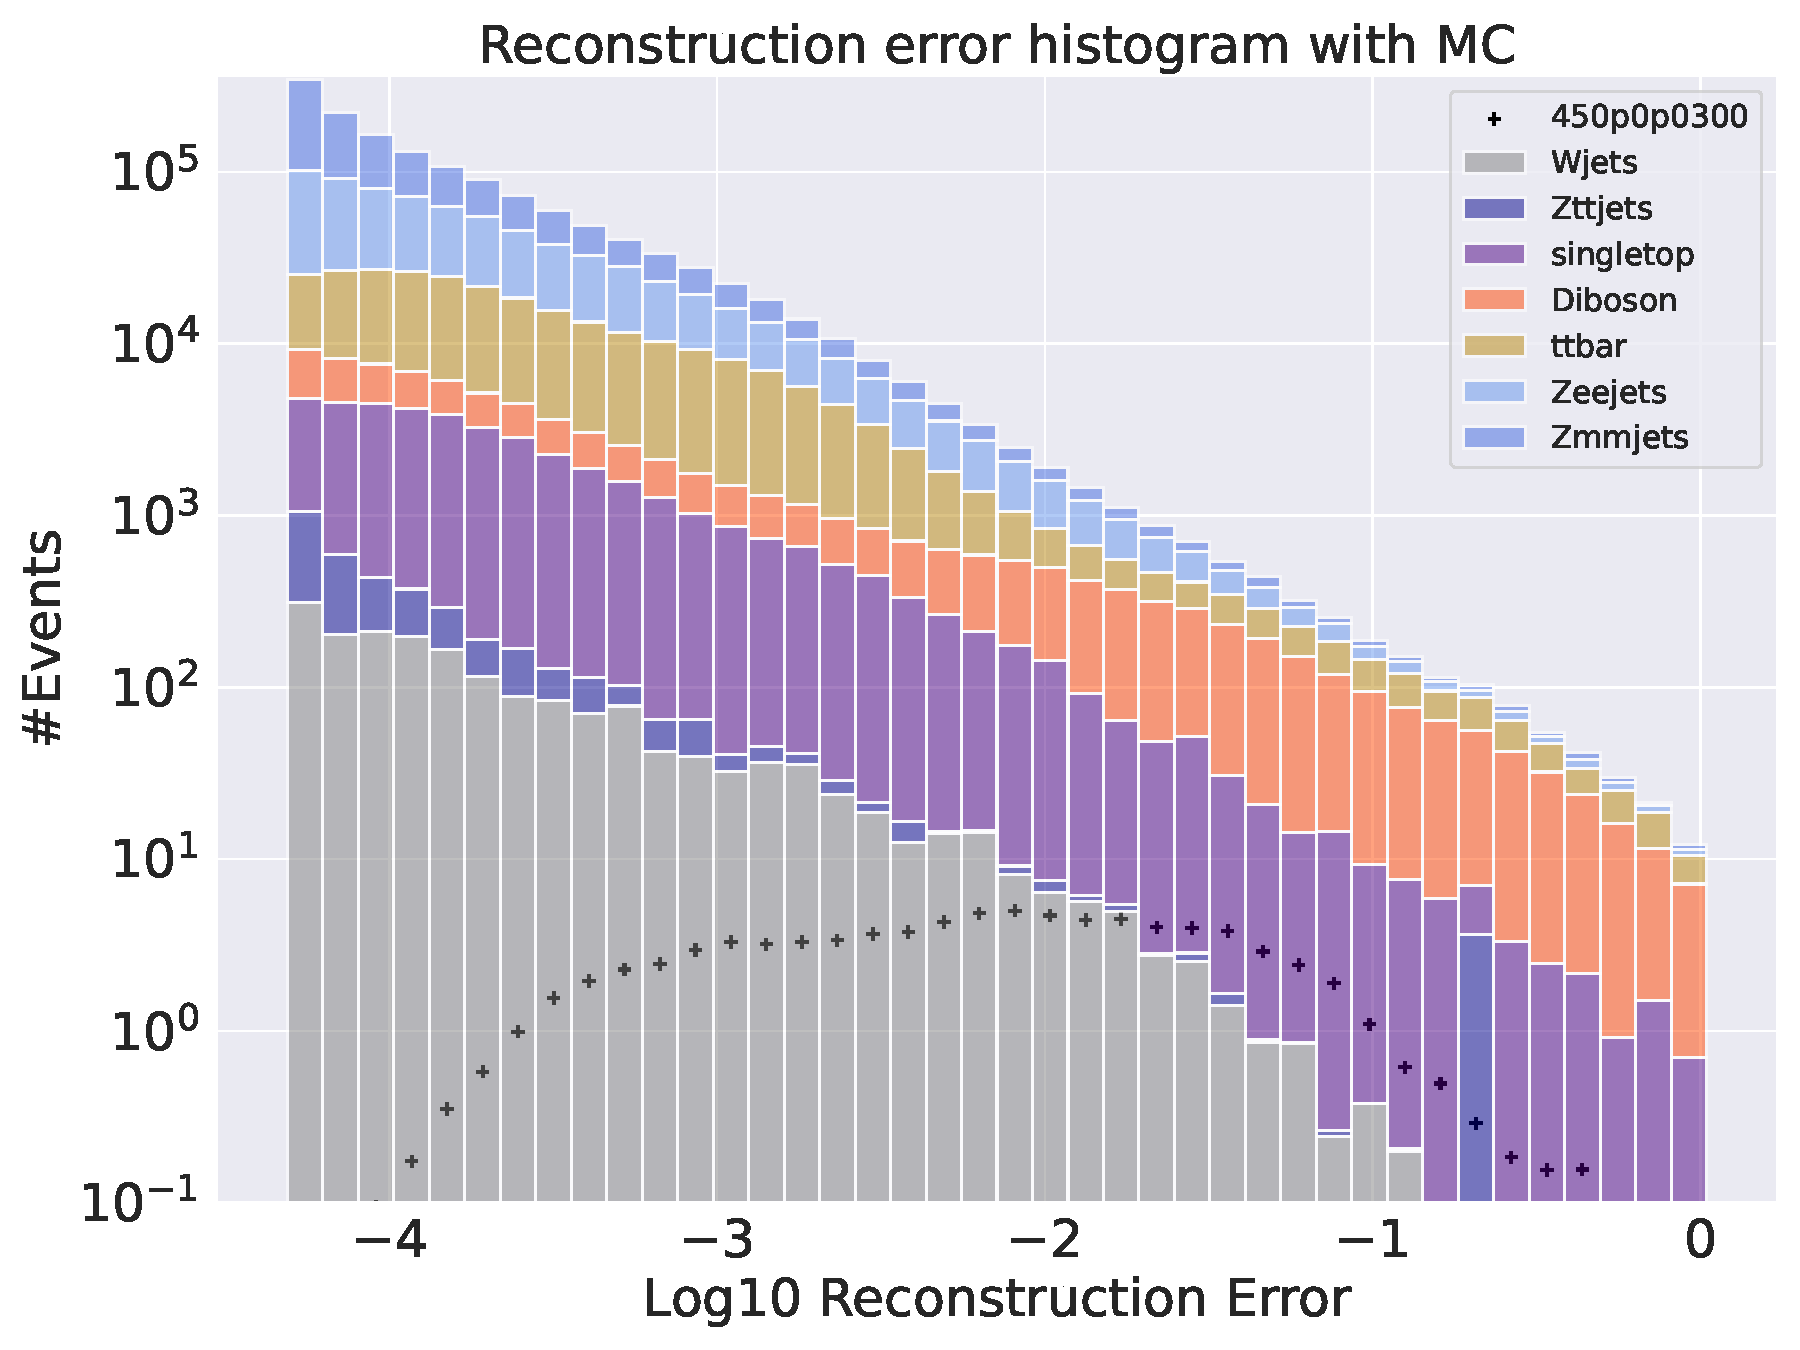
\includegraphics[width=\textwidth]{Figures/AE_testing/small/2lep/b_data_recon_big_rm3_feats_sig_450p0p0300_.pdf}
        \caption{ }
        \label{fig:AE_2lep_big_450}
    \end{subfigure}
    \hfill
    \begin{subfigure}{.45\textwidth}
        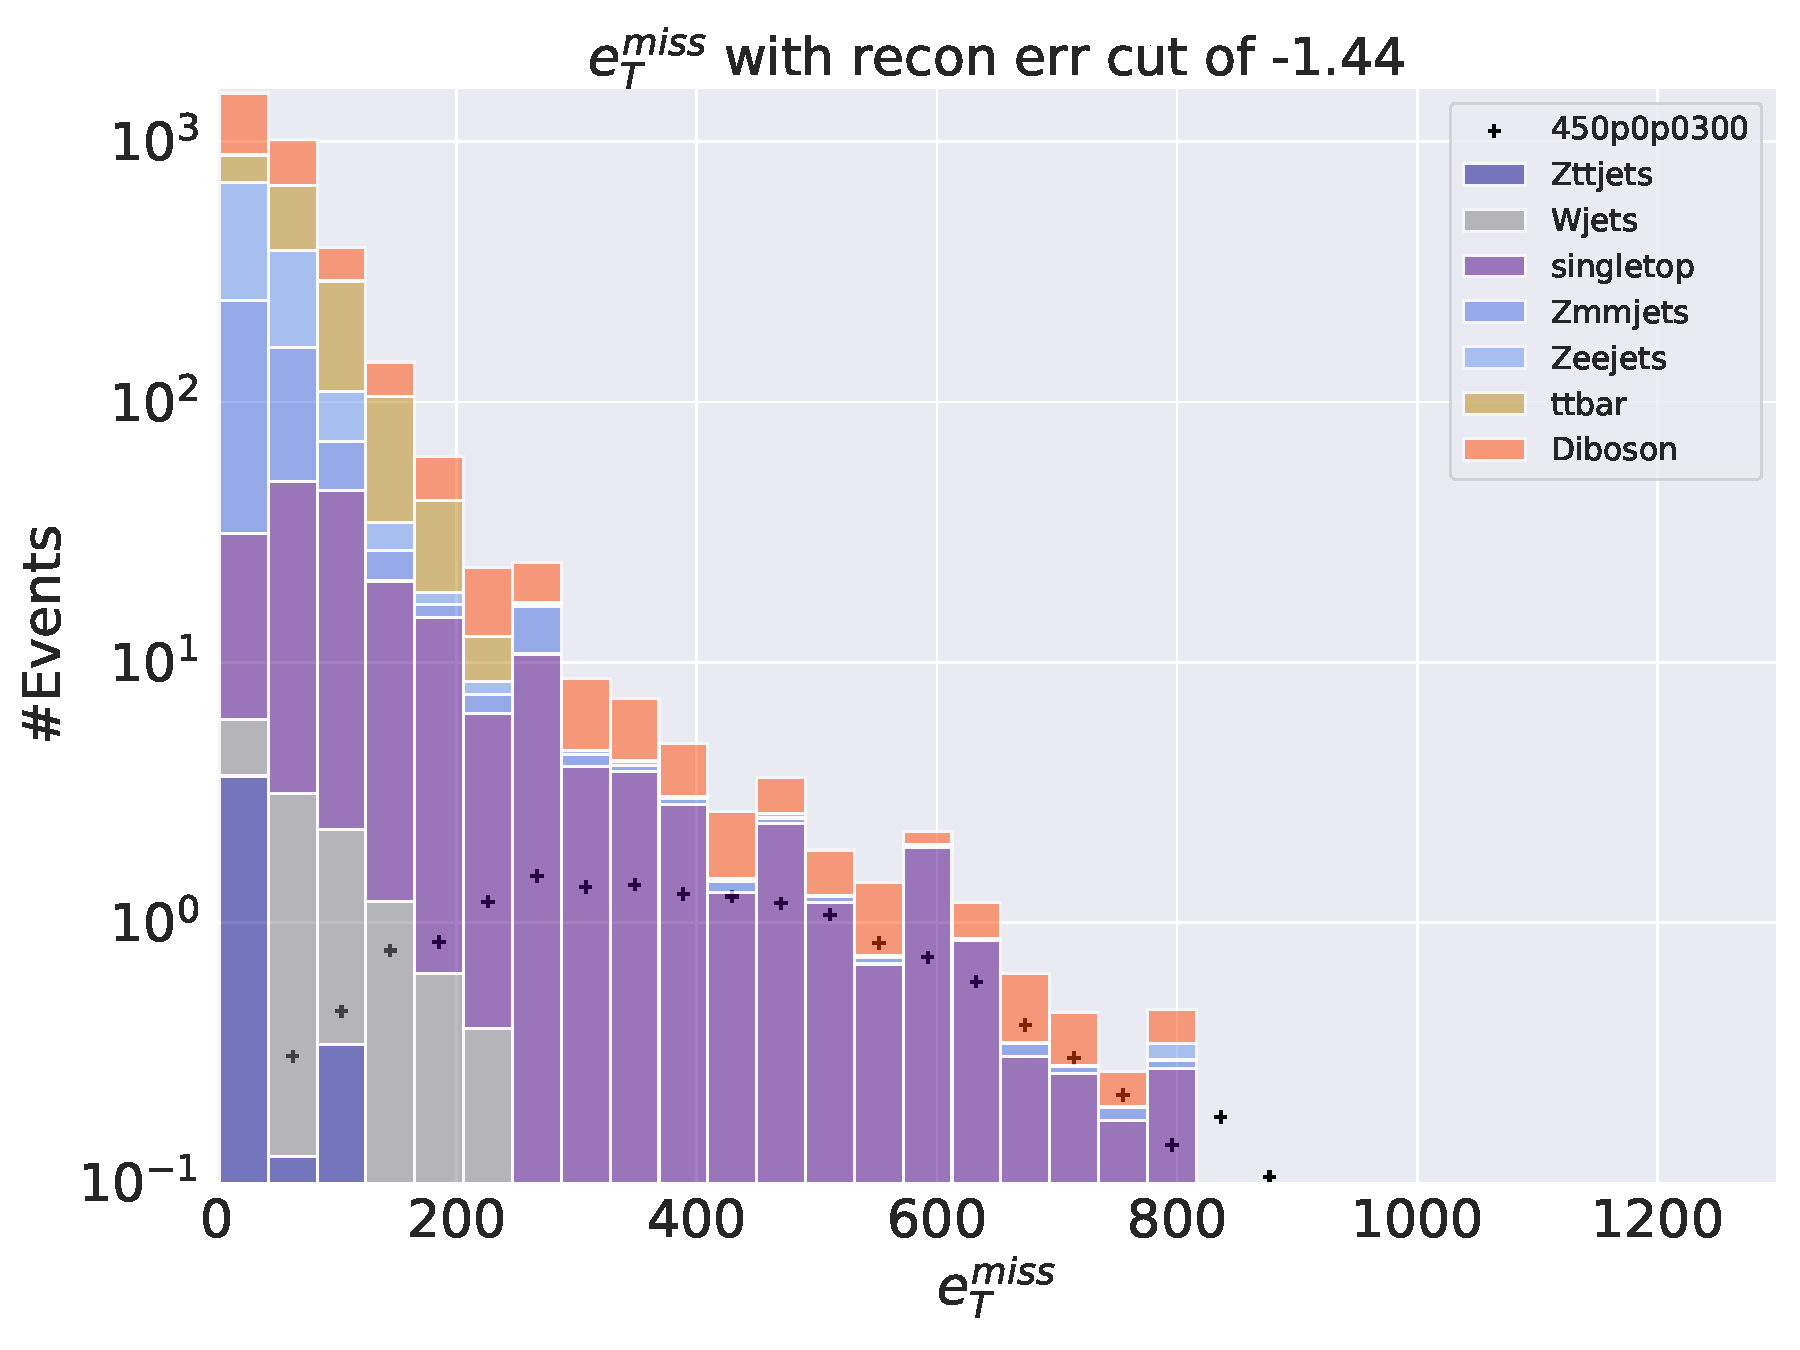
\includegraphics[width=\textwidth]{Figures/AE_testing/big/2lep/b_data_recon_big_rm3_feats_sig_450p0p0300_recon_errcut_-1.44.pdf}
        \caption{}
        \label{fig:AE_2lep_big_etmiss_450}
    \end{subfigure}
    \hfill 
    \begin{subfigure}{.45\textwidth}
        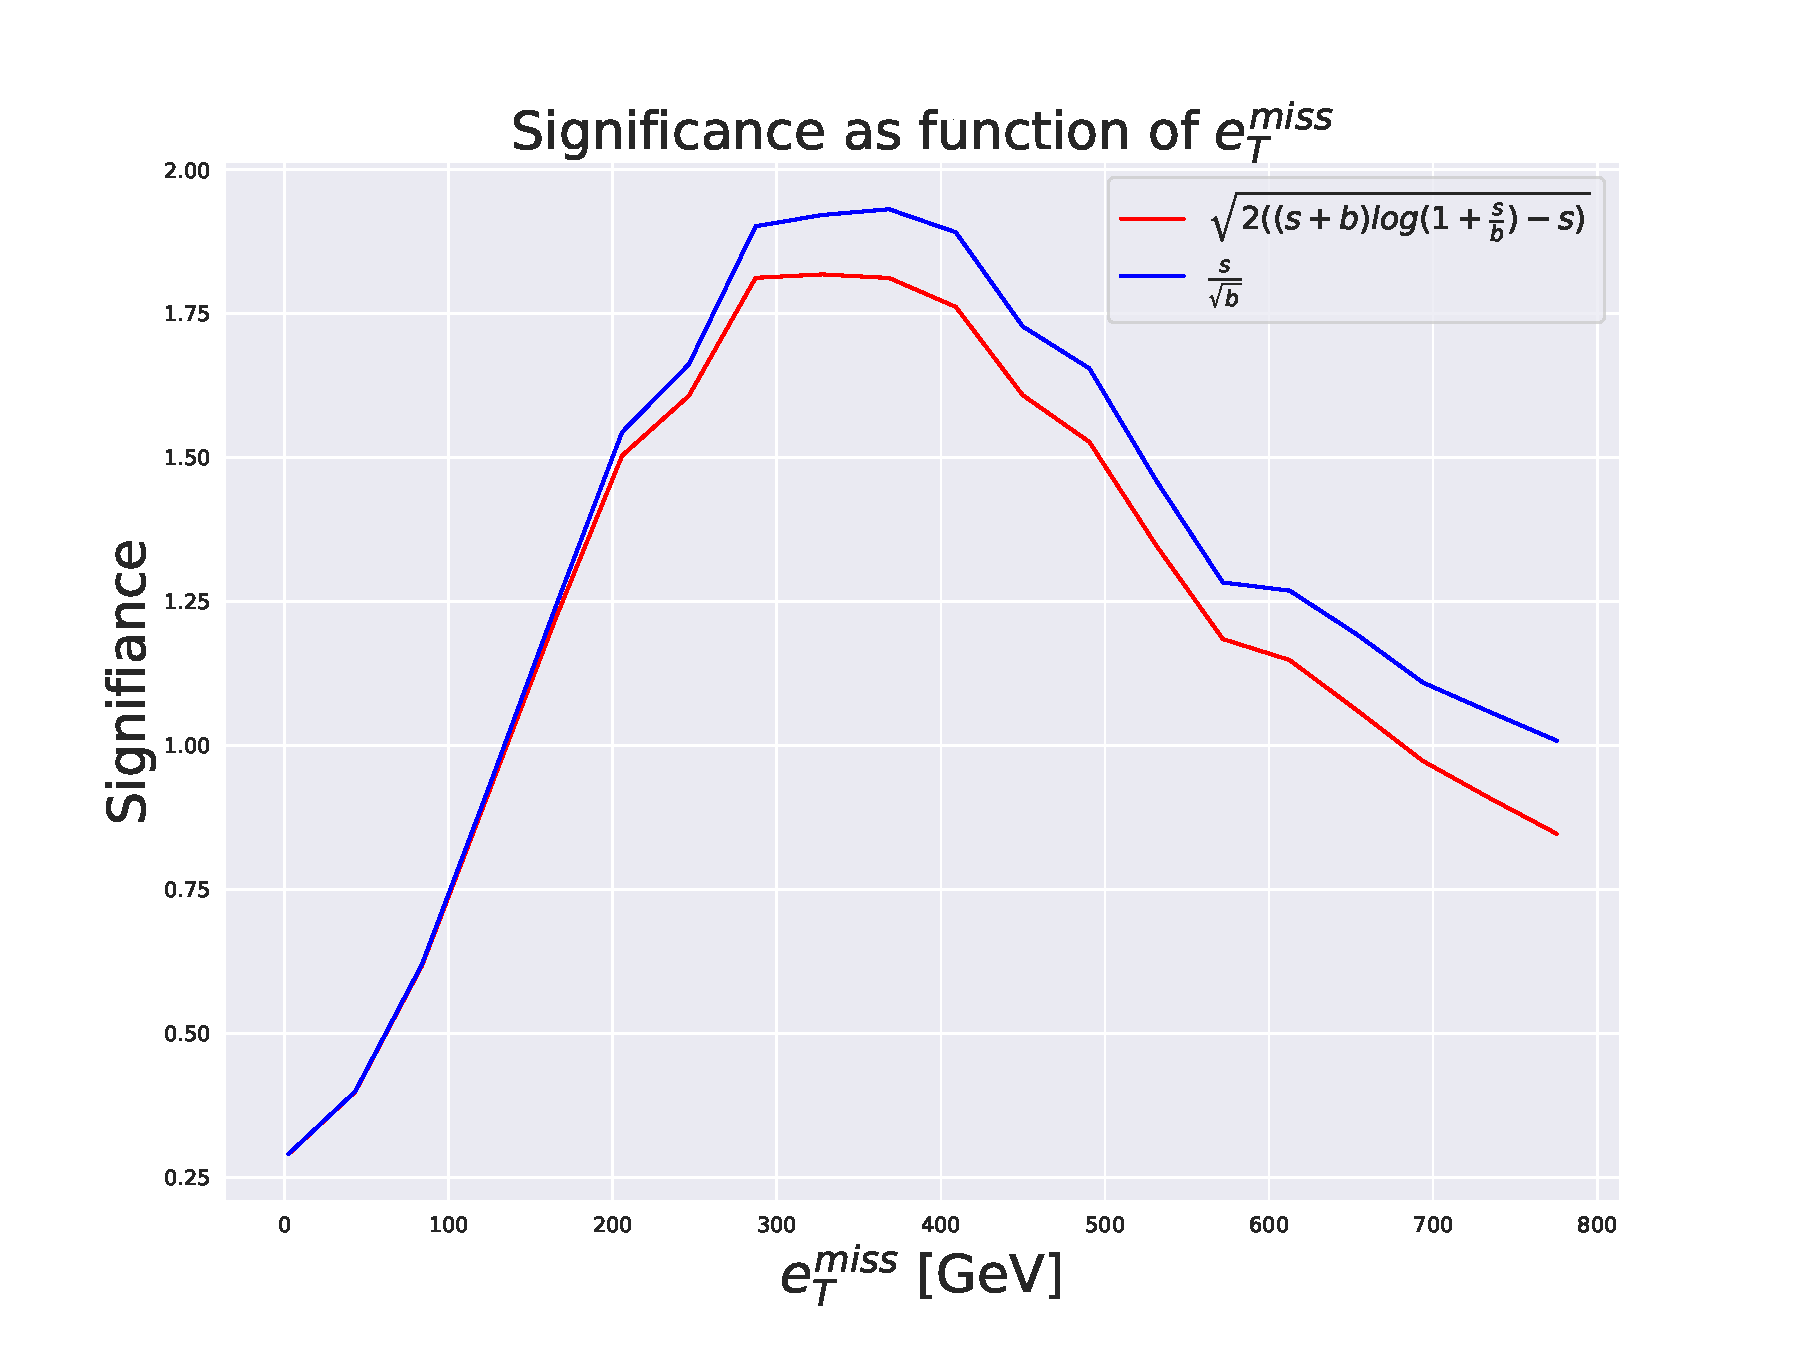
\includegraphics[width=\textwidth]{Figures/AE_testing/big/2lep/significance_etmiss_450p0p0300_-1.4360553938127363.pdf}
        \caption{}
        \label{fig:AE_2lep_big_signi_450}
    \end{subfigure}
    \hfill      
    \caption[2lep deep network | $450p300$ | AE]{Reconstruction error, $e_T^{miss}$ signal region, $m_{lll}$ signal region and significance as function of 
    $e_T^{miss}$ for the deep regular autoencoder using SUSY $450p300$. In figures \ref{fig:AE_2lep_big_450} there is a general trend here for both the small and large regular 
    autoencoder where the background distributions are highly shifted to the lower end of the 
    reconstruction error range. As the reconstruction error increases, the amount of each sample in a 
    given bin changes alot. In figure \ref{fig:AE_2lep_big_etmiss_450} there is a small separation between the peaks of the background
    and the signal. There is still mostly overlap between the two distributions. }
    \label{fig:AE_2lep_big_rec_sig_signi_450}
\end{figure}

\begin{figure}[H]
    \centering
    \begin{subfigure}{.45\textwidth}
        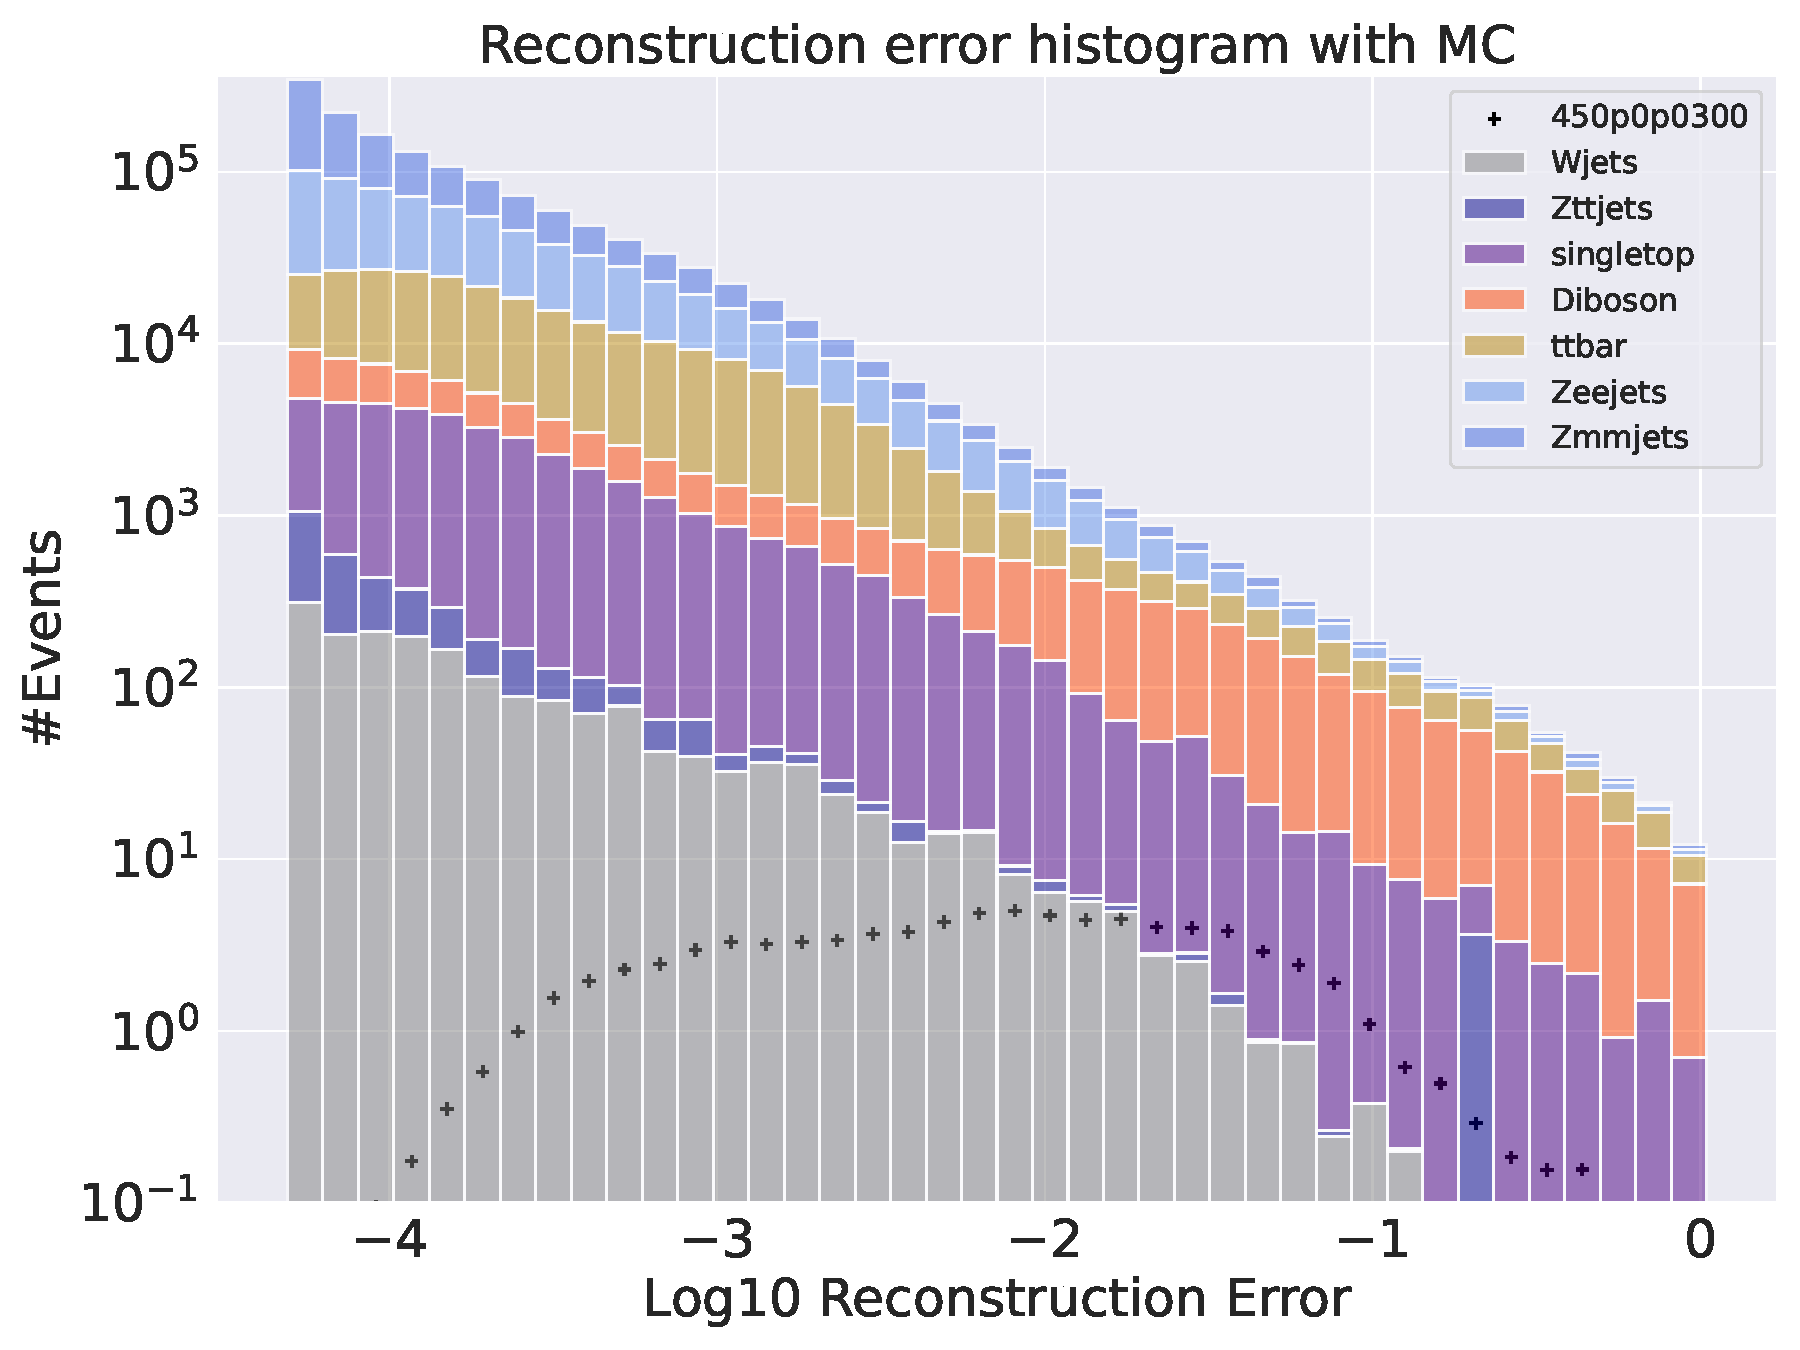
\includegraphics[width=\textwidth]{Figures/AE_testing/small/2lep/b_data_recon_big_rm3_feats_sig_450p0p0300_.pdf}
        \caption{ }
        \label{fig:AE_2lep_small_450}
    \end{subfigure}
    \hfill
    \begin{subfigure}{.45\textwidth}
        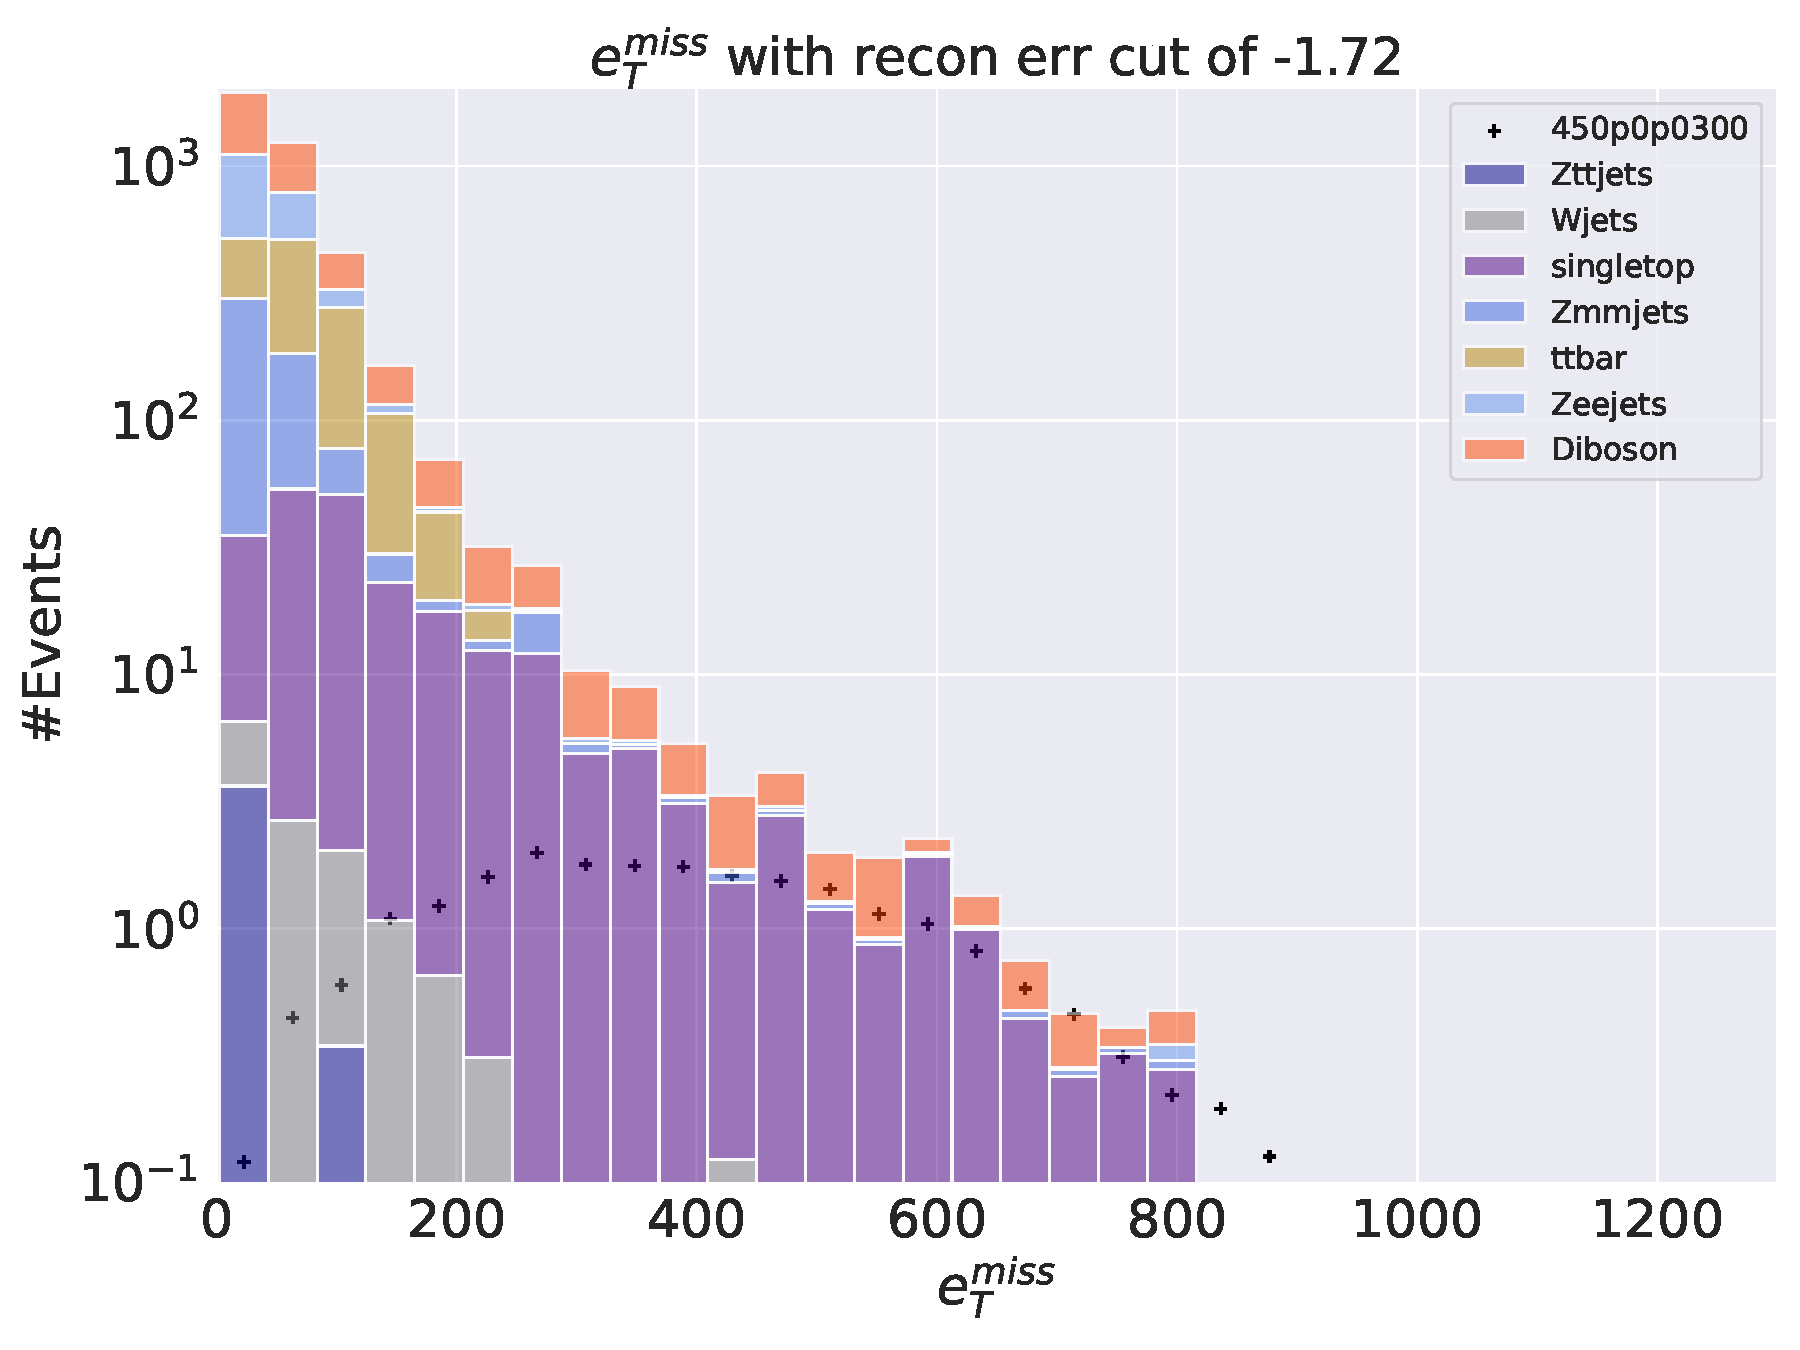
\includegraphics[width=\textwidth]{Figures/AE_testing/small/2lep/b_data_recon_big_rm3_feats_sig_450p0p0300_recon_errcut_-1.72.pdf}
        \caption{}
        \label{fig:AE_2lep_small_etmiss_450}
    \end{subfigure}
    \hfill  
    \begin{subfigure}{.45\textwidth}
        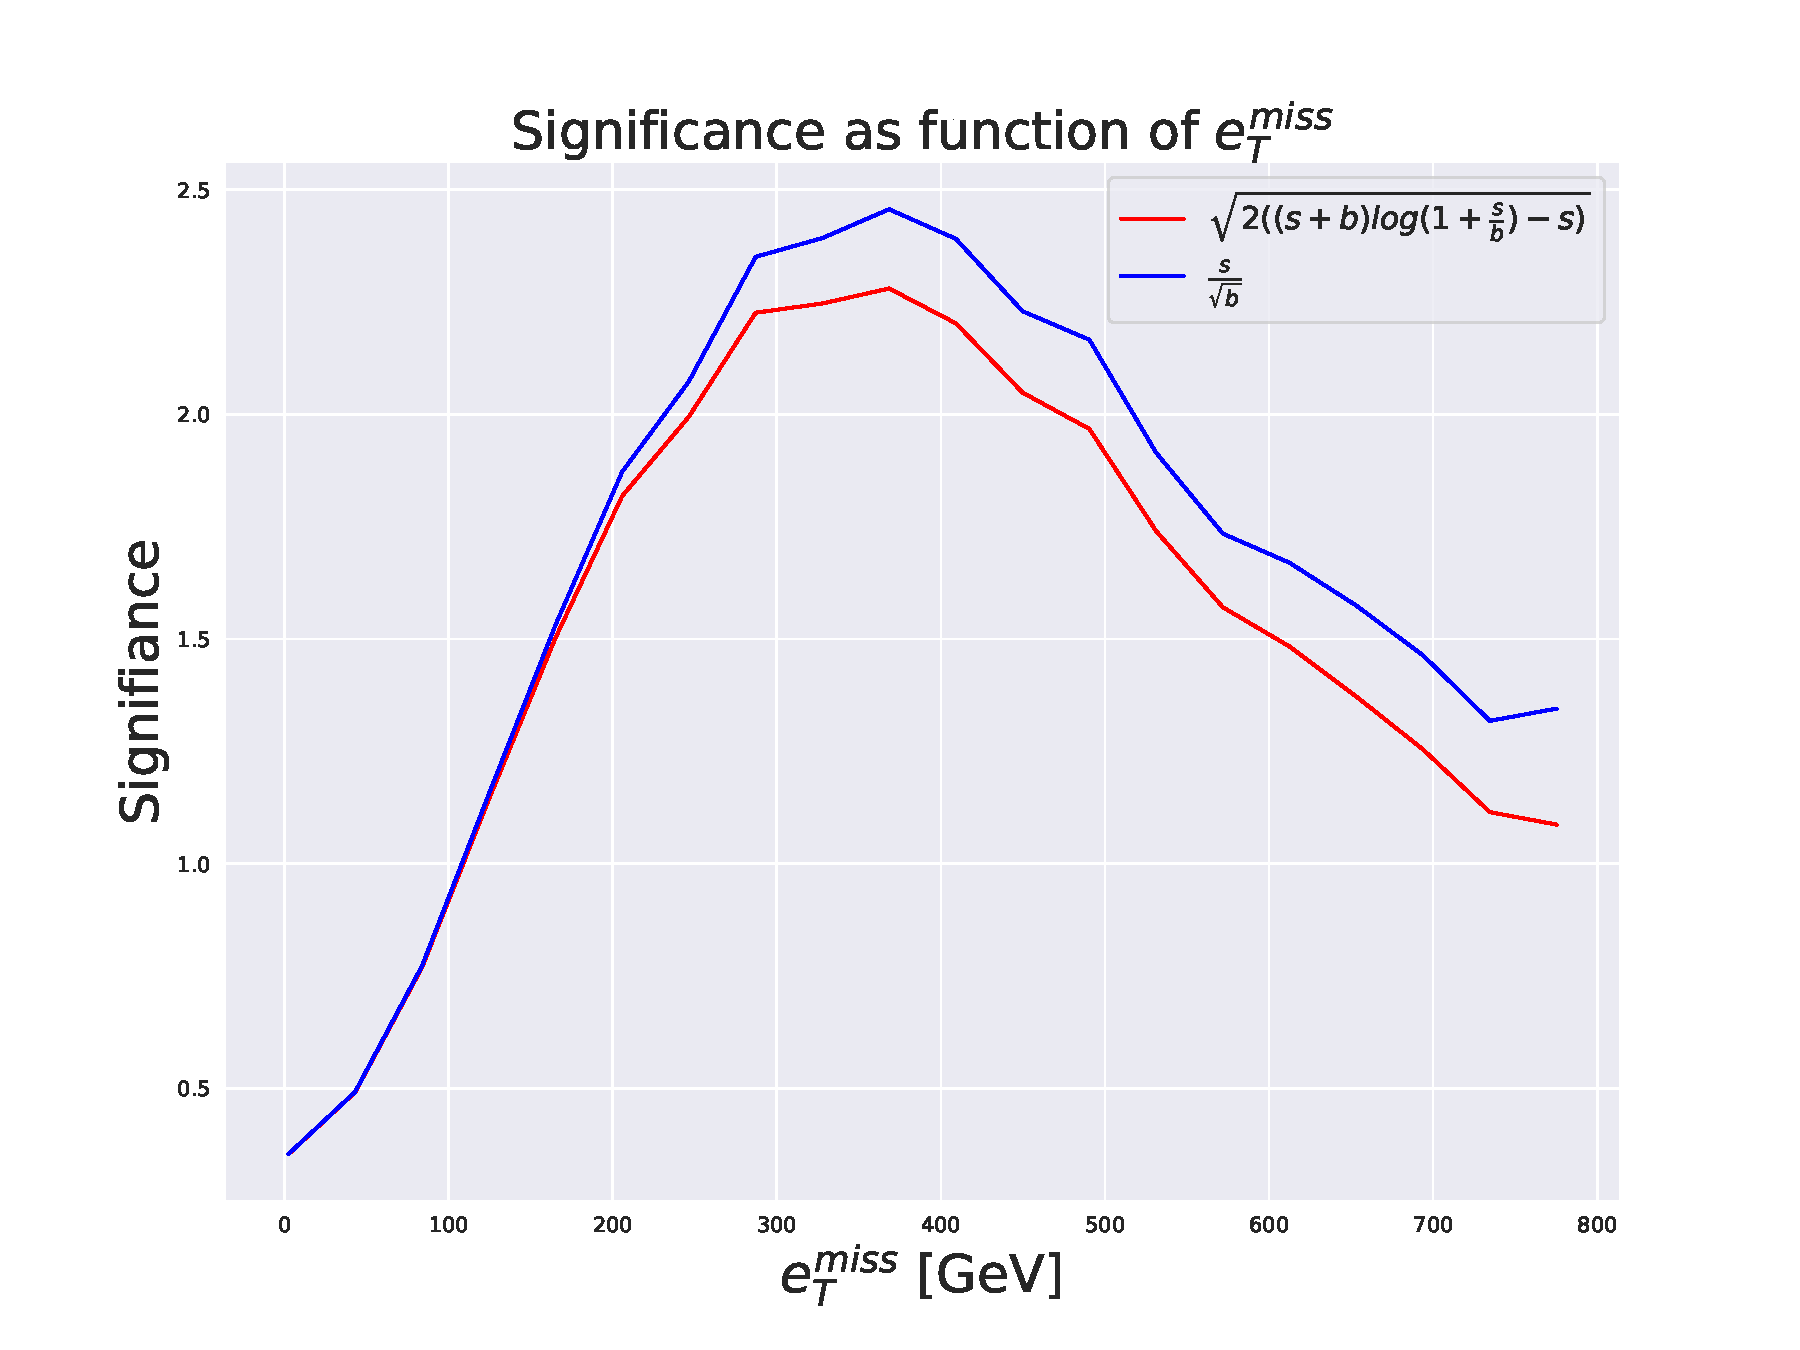
\includegraphics[width=\textwidth]{Figures/AE_testing/small/2lep/significance_etmiss_450p0p0300_-1.7167506533614734.pdf}
        \caption{}
        \label{fig:AE_2lep_small_signi_450}
    \end{subfigure}
    \hfill      
    \caption[2lep shallow network | $450p300$ | AE]{Reconstruction error, $e_T^{miss}$ signal region, $m_{lll}$ signal region and significance as function of 
    $e_T^{miss}$ for the deep regular autoencoder using SUSY $450p300$. In figures \ref{fig:AE_2lep_small_450} there is a general trend here for both the small and large regular 
    autoencoder where the background distributions are highly shifted to the lower end of the 
    reconstruction error range. As the reconstruction error increases, the amount of each sample in a 
    given bin changes alot. In figure \ref{fig:AE_2lep_small_etmiss_450} there is a small separation between the peaks of the background
    and the signal. There is still mostly overlap between the two distributions.}
    \label{fig:AE_2lep_small_rec_sig_signi_450}
\end{figure}


\begin{figure}[H]
    \centering
    \begin{subfigure}{.45\textwidth}
        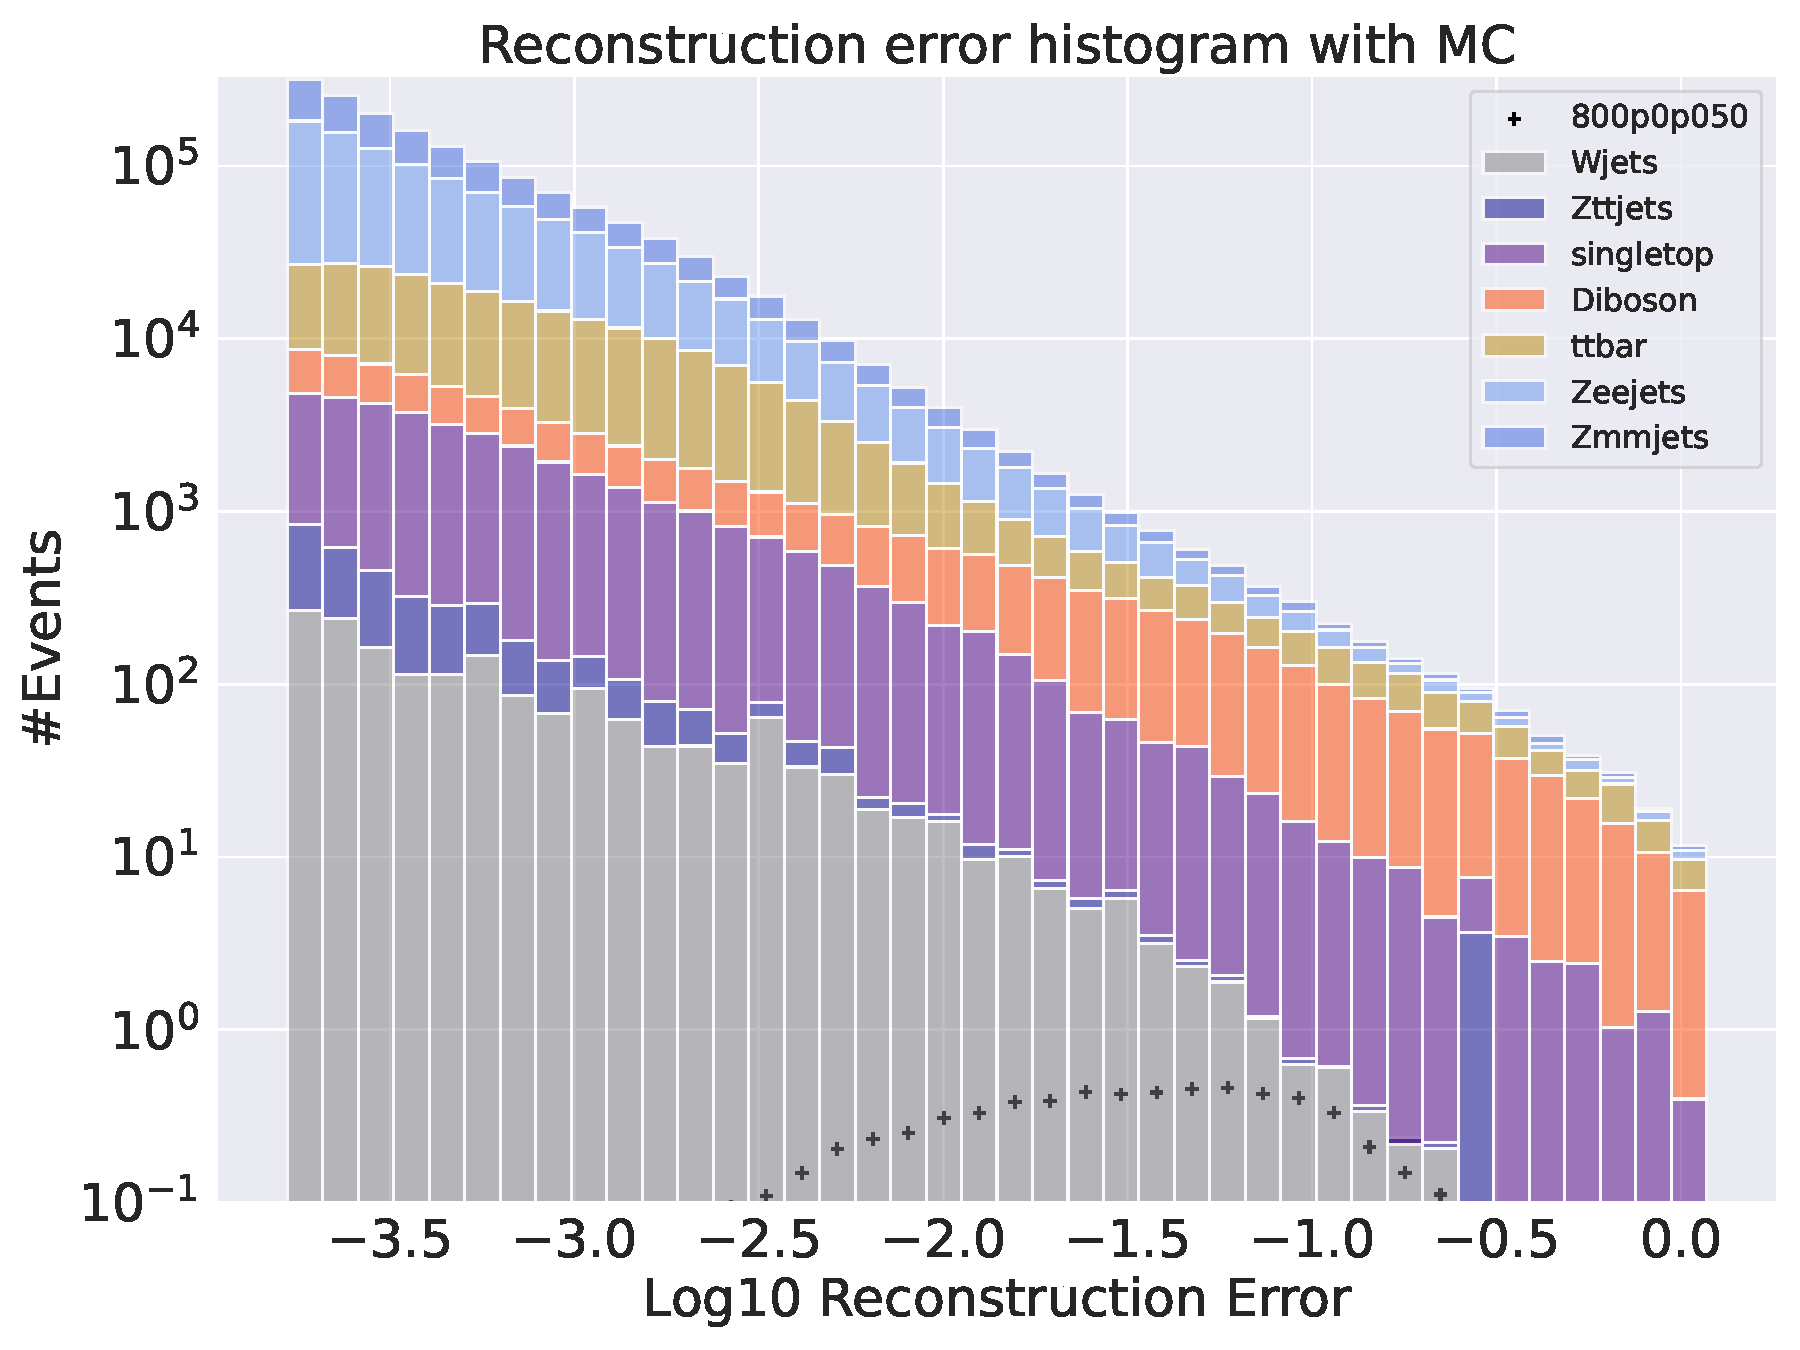
\includegraphics[width=\textwidth]{Figures/AE_testing/big/2lep/b_data_recon_big_rm3_feats_sig_800p0p050_.pdf}
        \caption{ }
        \label{fig:AE_2lep_big_800}
    \end{subfigure}
    \hfill
    \begin{subfigure}{.45\textwidth}
        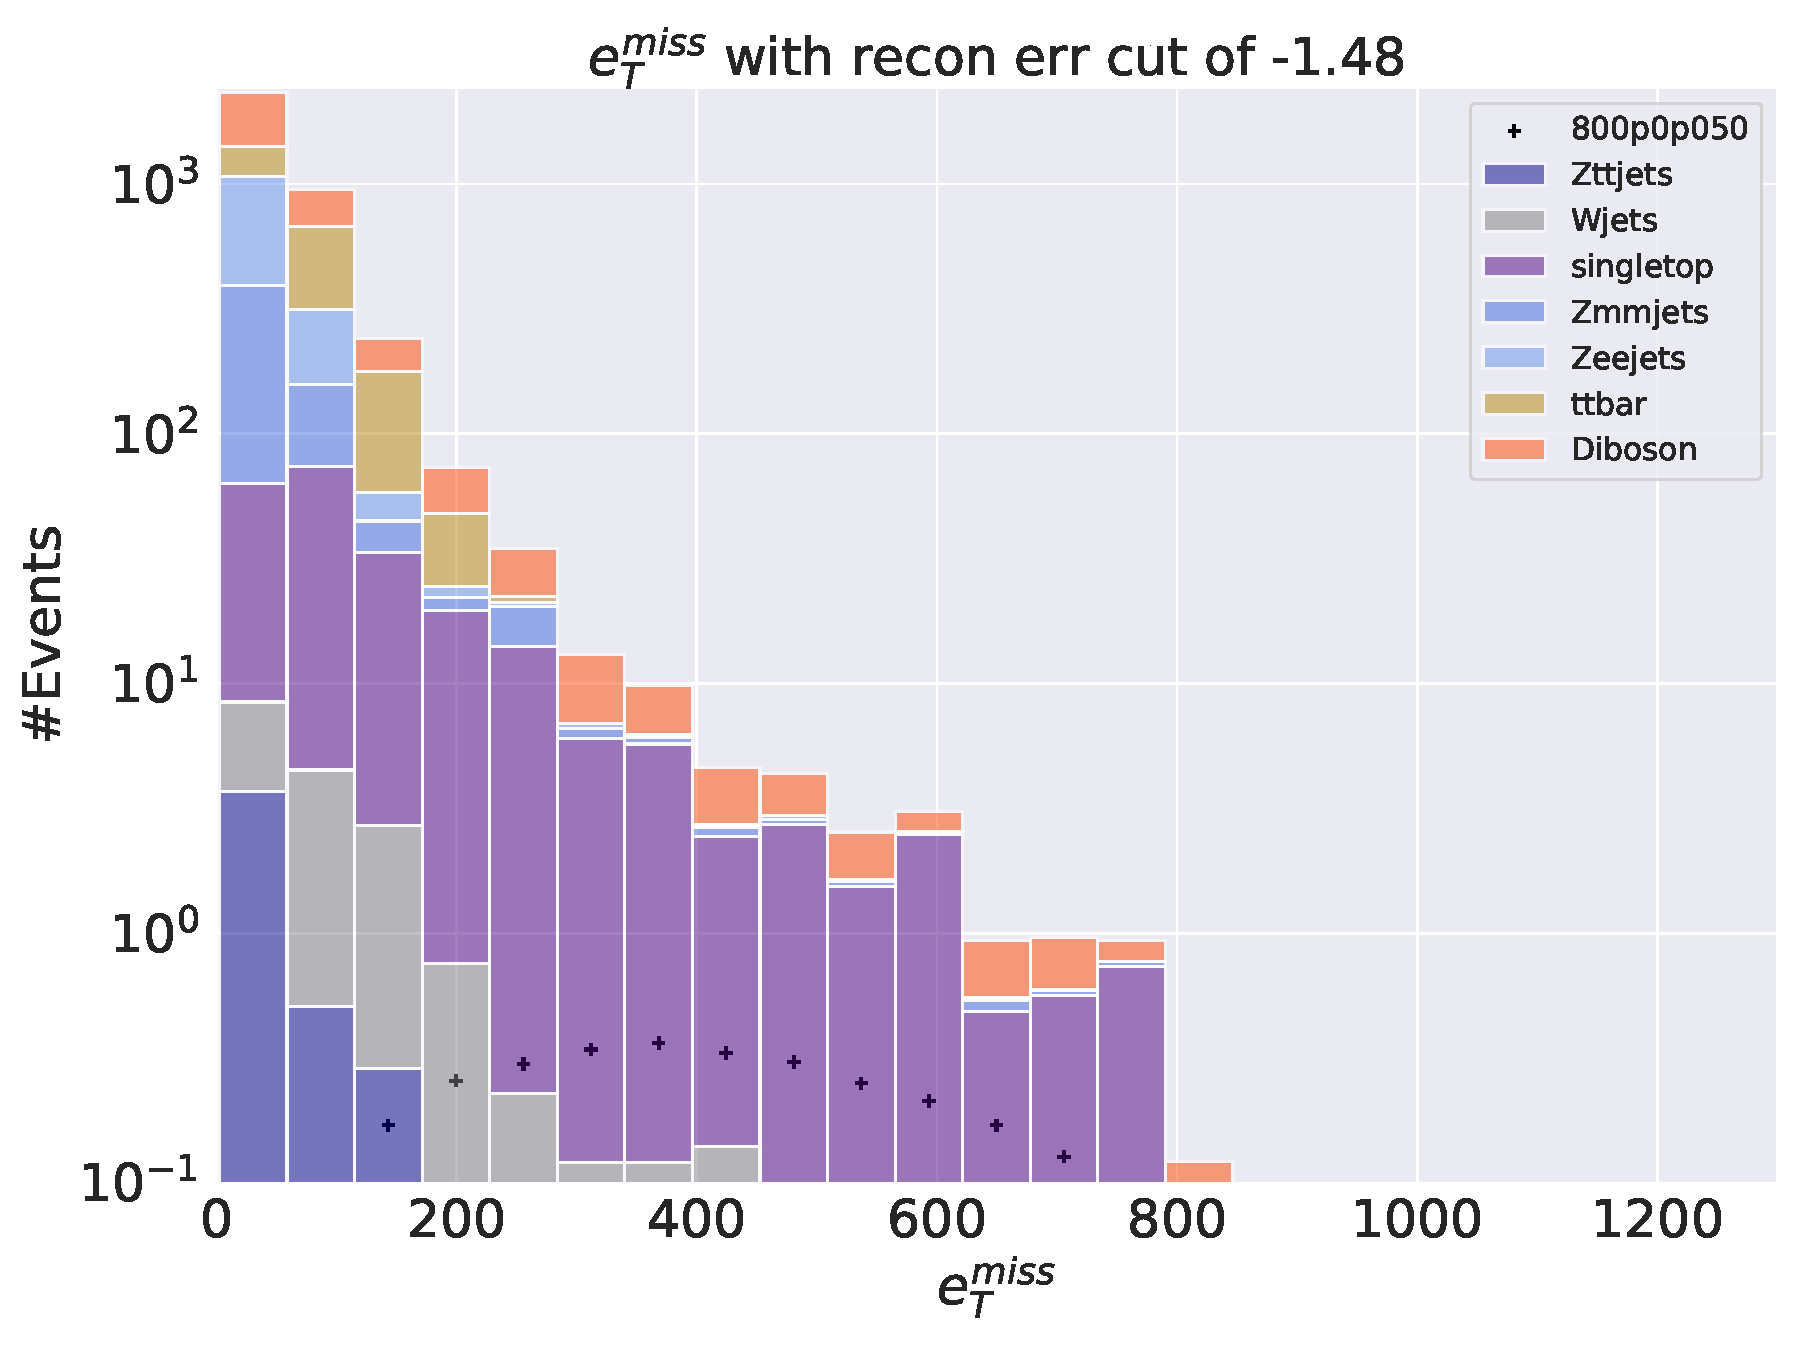
\includegraphics[width=\textwidth]{Figures/AE_testing/big/2lep/b_data_recon_big_rm3_feats_sig_800p0p050_recon_errcut_-1.48.pdf}
        \caption{}
        \label{fig:AE_2lep_big_etmiss_800}
    \end{subfigure}
    \hfill
      
    \begin{subfigure}{.45\textwidth}
        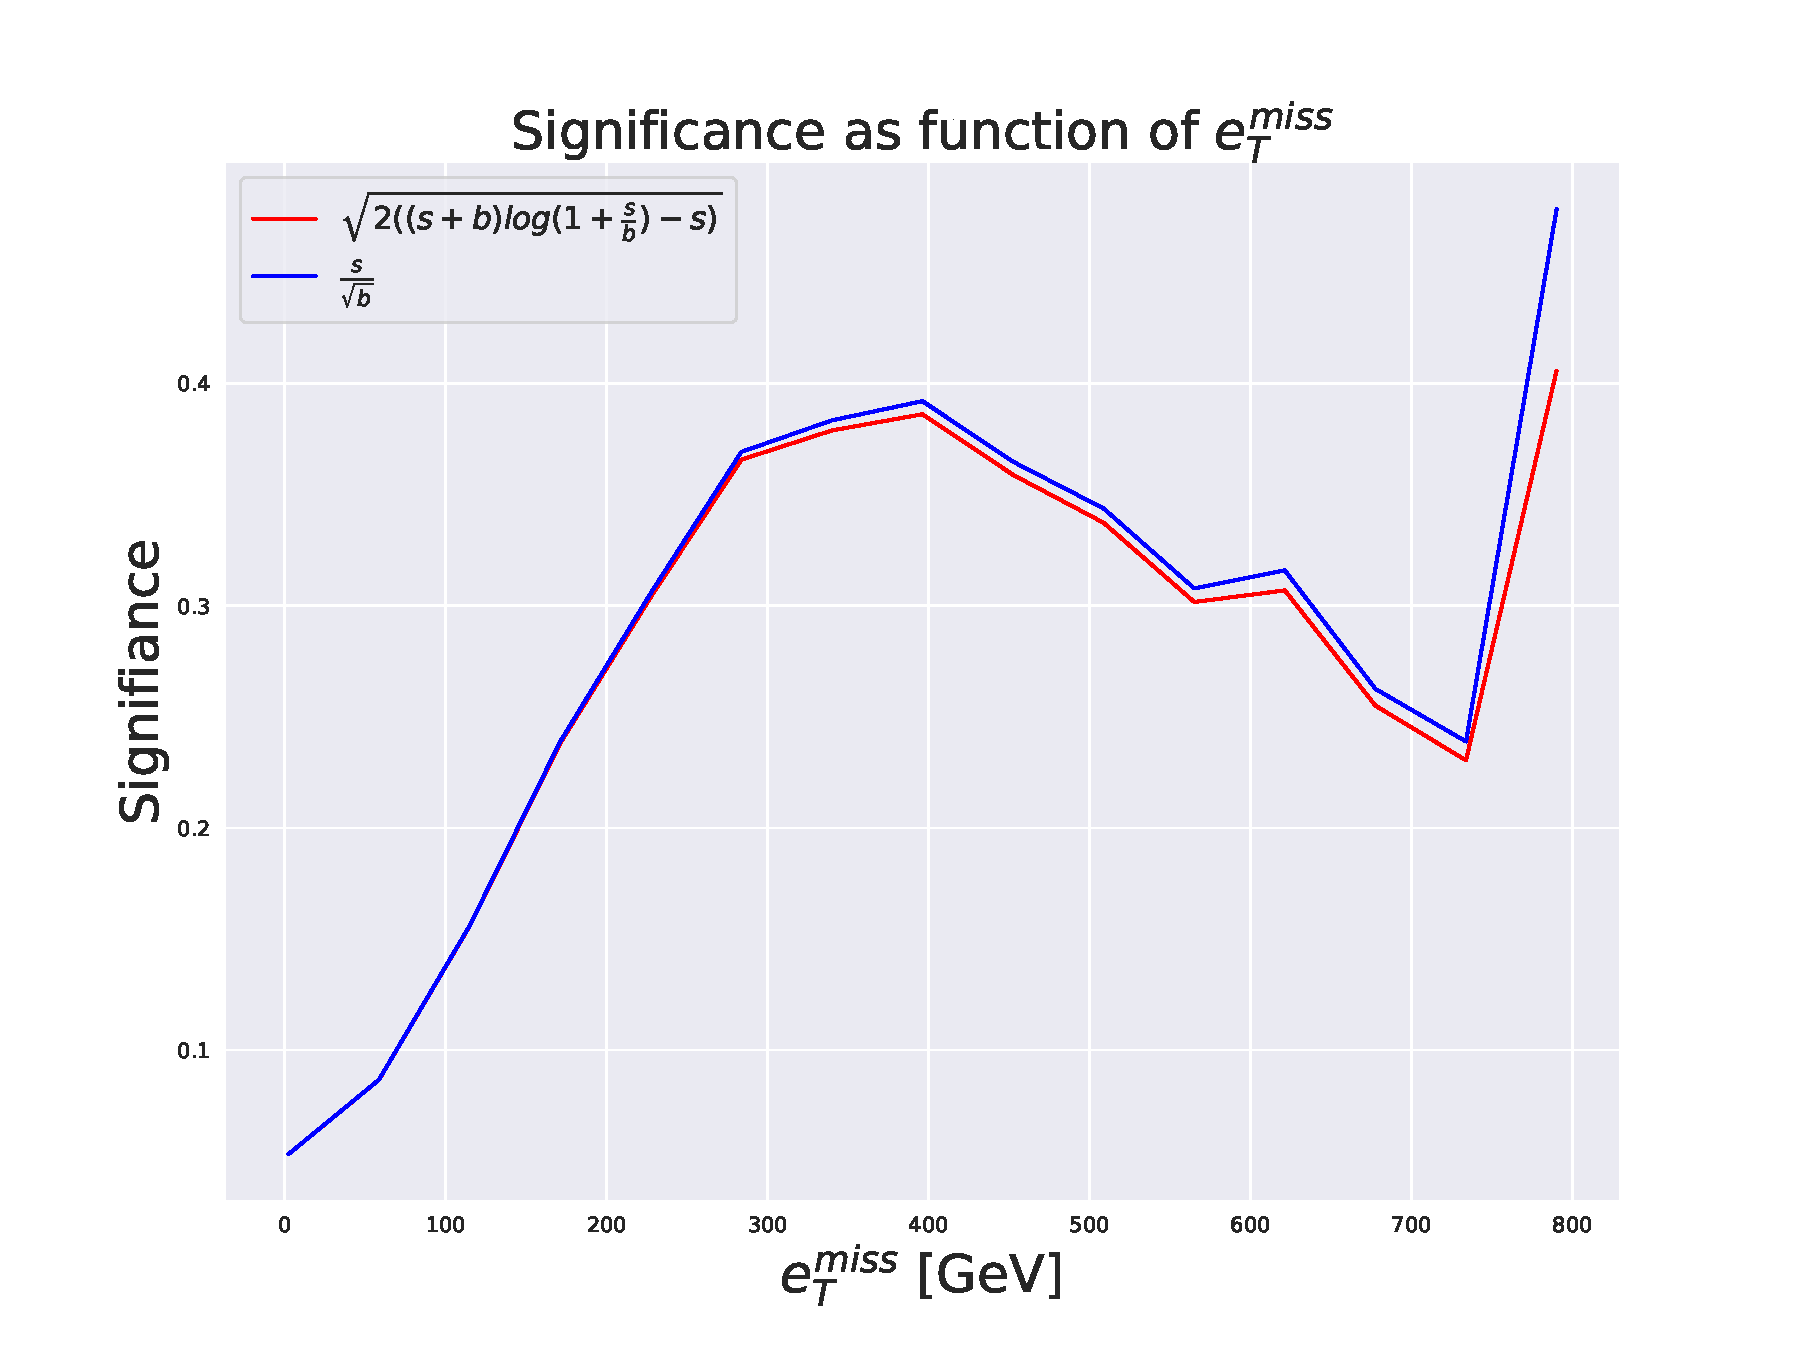
\includegraphics[width=\textwidth]{Figures/AE_testing/big/2lep/significance_etmiss_800p0p050_-1.4833711230716062.pdf}
        \caption{}
        \label{fig:AE_2lep_big_signi_800}
    \end{subfigure}
    \hfill      
    \caption[2lep deep network | $800p50$ | AE]{Reconstruction error, $e_T^{miss}$ signal region, $m_{lll}$ signal region and significance as function of 
    $e_T^{miss}$ for the deep regular autoencoder using SUSY $800p50$. In figures  \ref{fig:AE_2lep_big_800}, 
    there is a general trend here for both the small and large regular 
    autoencoder where the background distributions are highly shifted to the lower end of the 
    reconstruction error range. As the reconstruction error increases, the amount of each sample in a 
    given bin changes alot. In figure \ref{fig:AE_2lep_big_etmiss_800} and  
    there is a small separation between the peaks of the background
    and the signal. There is still mostly overlap between the two distributions.}
    \label{fig:AE_2lep_big_rec_sig_signi_800}
\end{figure}

\begin{figure}[H]
    \centering
    \begin{subfigure}{.45\textwidth}
        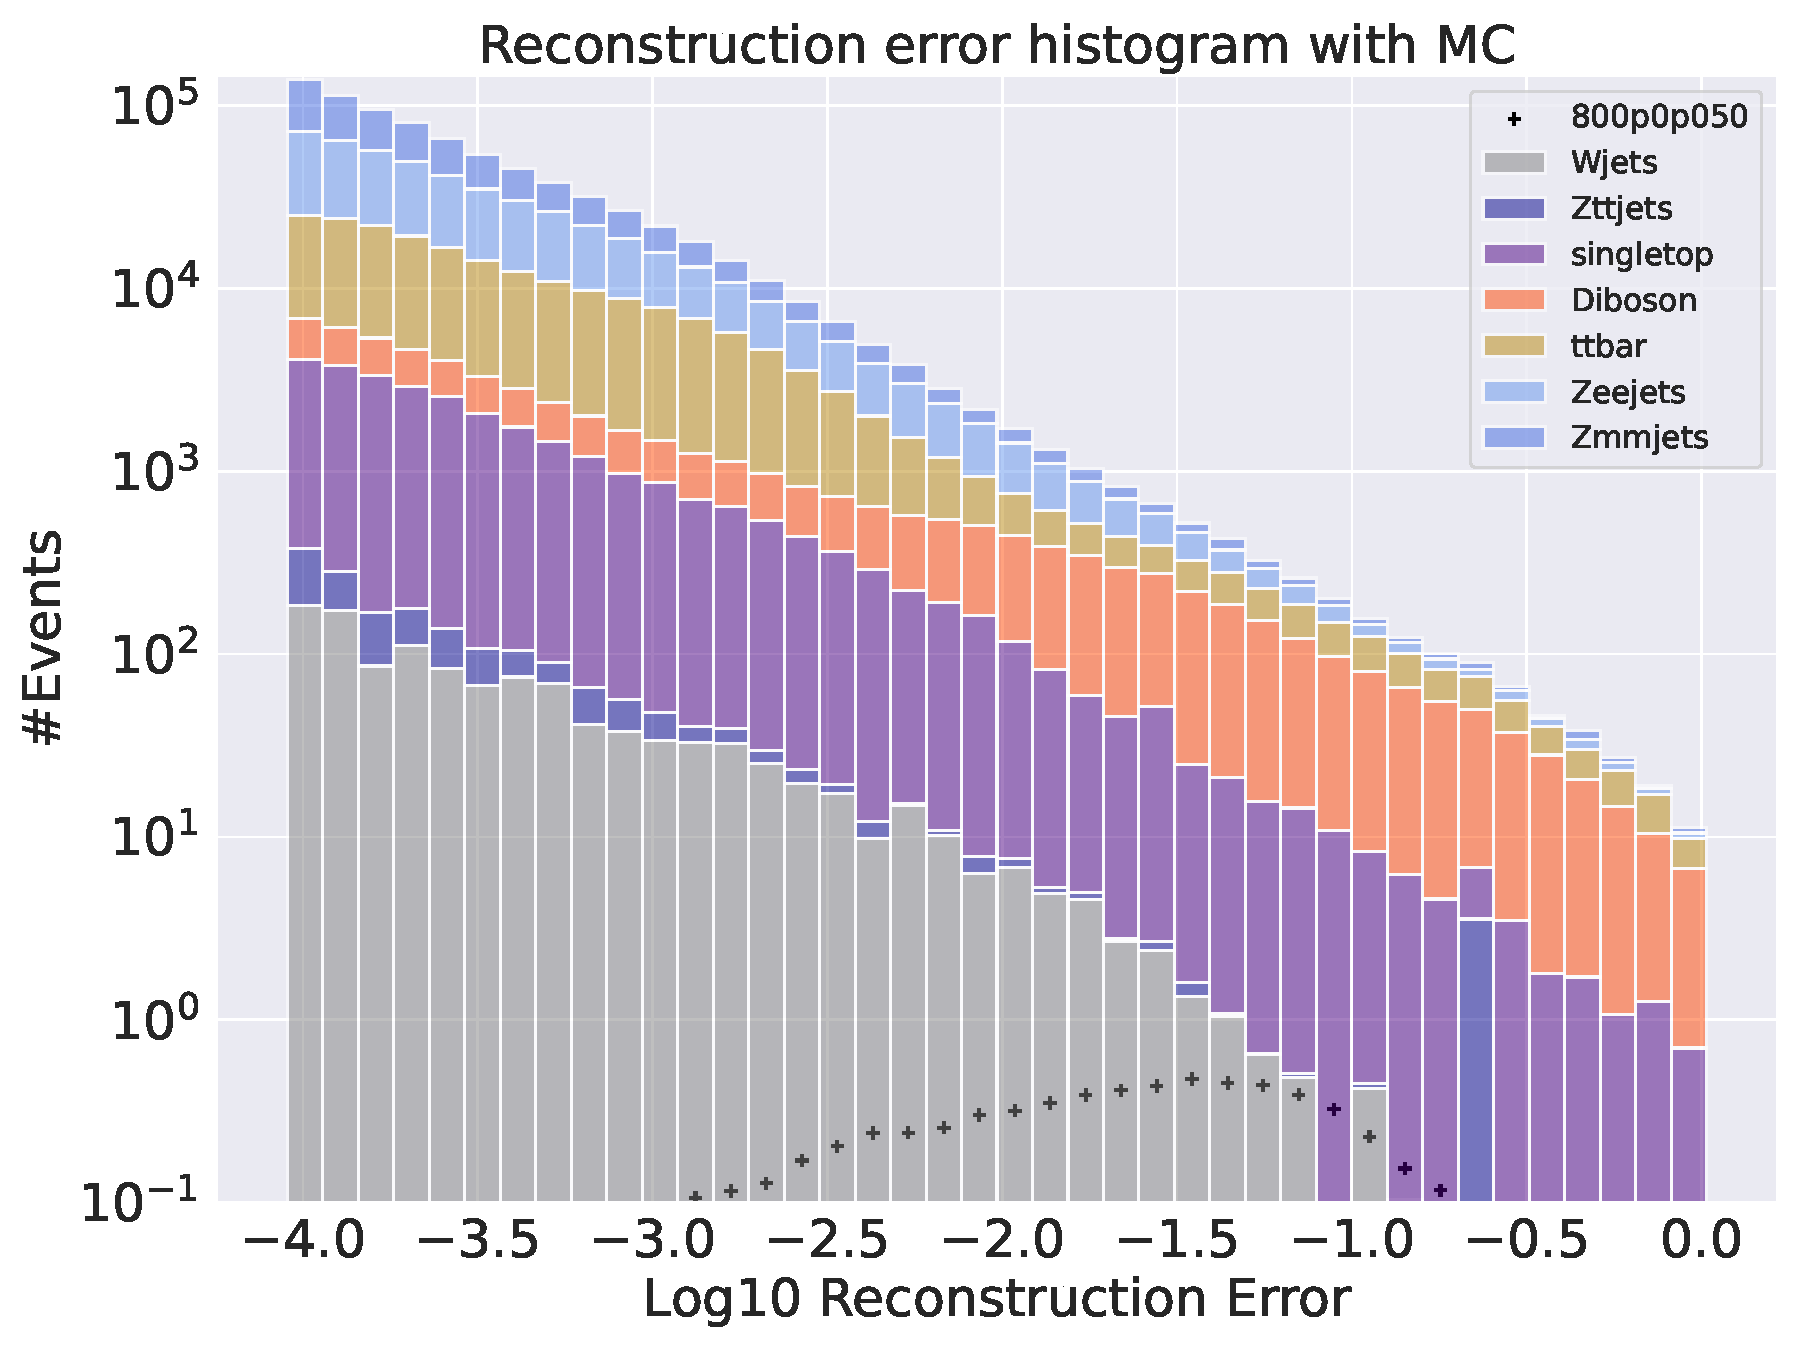
\includegraphics[width=\textwidth]{Figures/AE_testing/small/2lep/b_data_recon_big_rm3_feats_sig_800p0p050_.pdf}
        \caption{ }
        \label{fig:AE_2lep_small_800}
    \end{subfigure}
    \hfill
    \begin{subfigure}{.45\textwidth}
        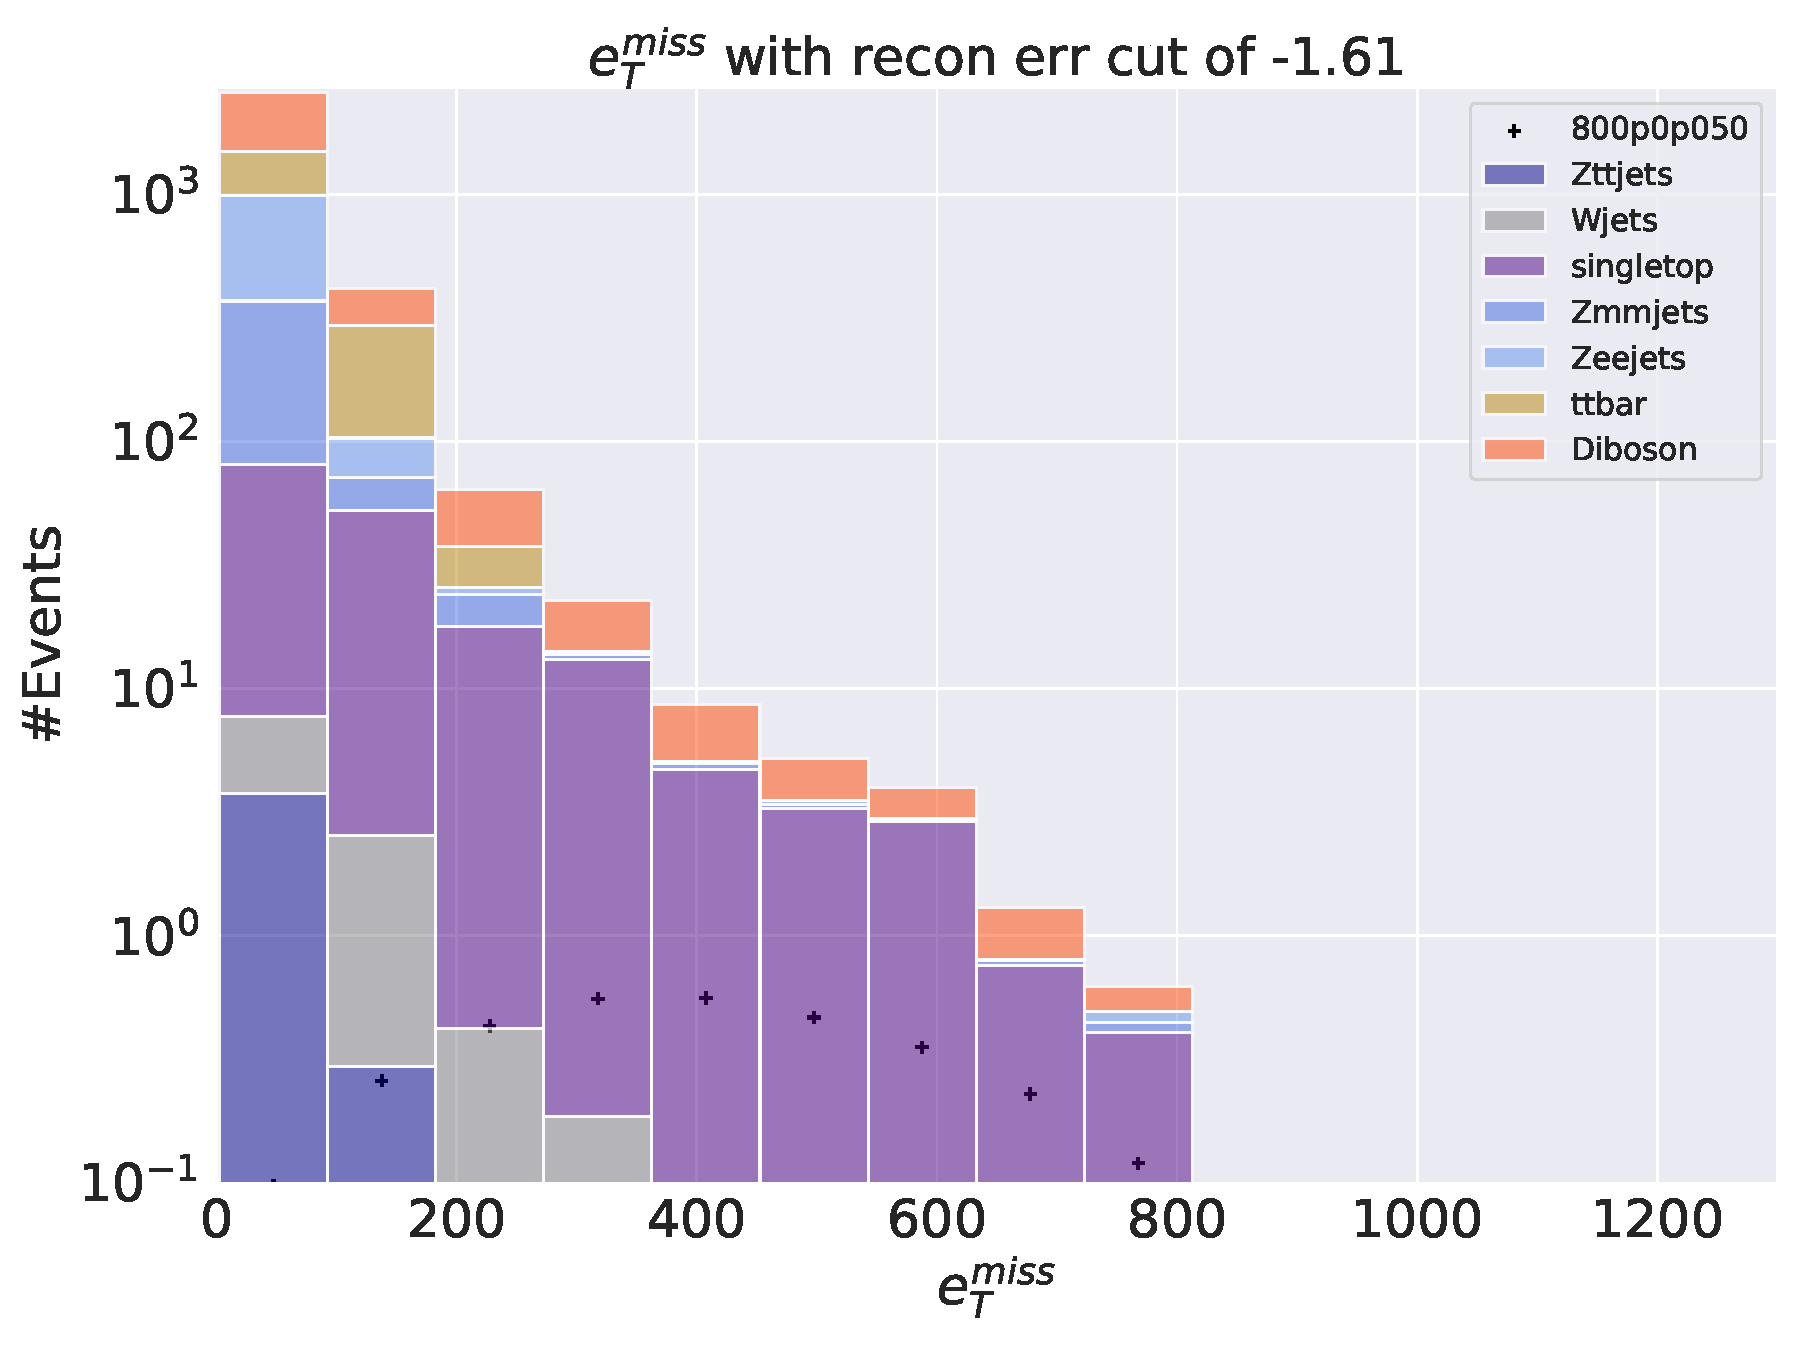
\includegraphics[width=\textwidth]{Figures/AE_testing/small/2lep/b_data_recon_big_rm3_feats_sig_800p0p050_recon_errcut_-1.61.pdf}
        \caption{}
        \label{fig:AE_2lep_small_etmiss_800}
    \end{subfigure}
    \hfill  
    \begin{subfigure}{.45\textwidth}
        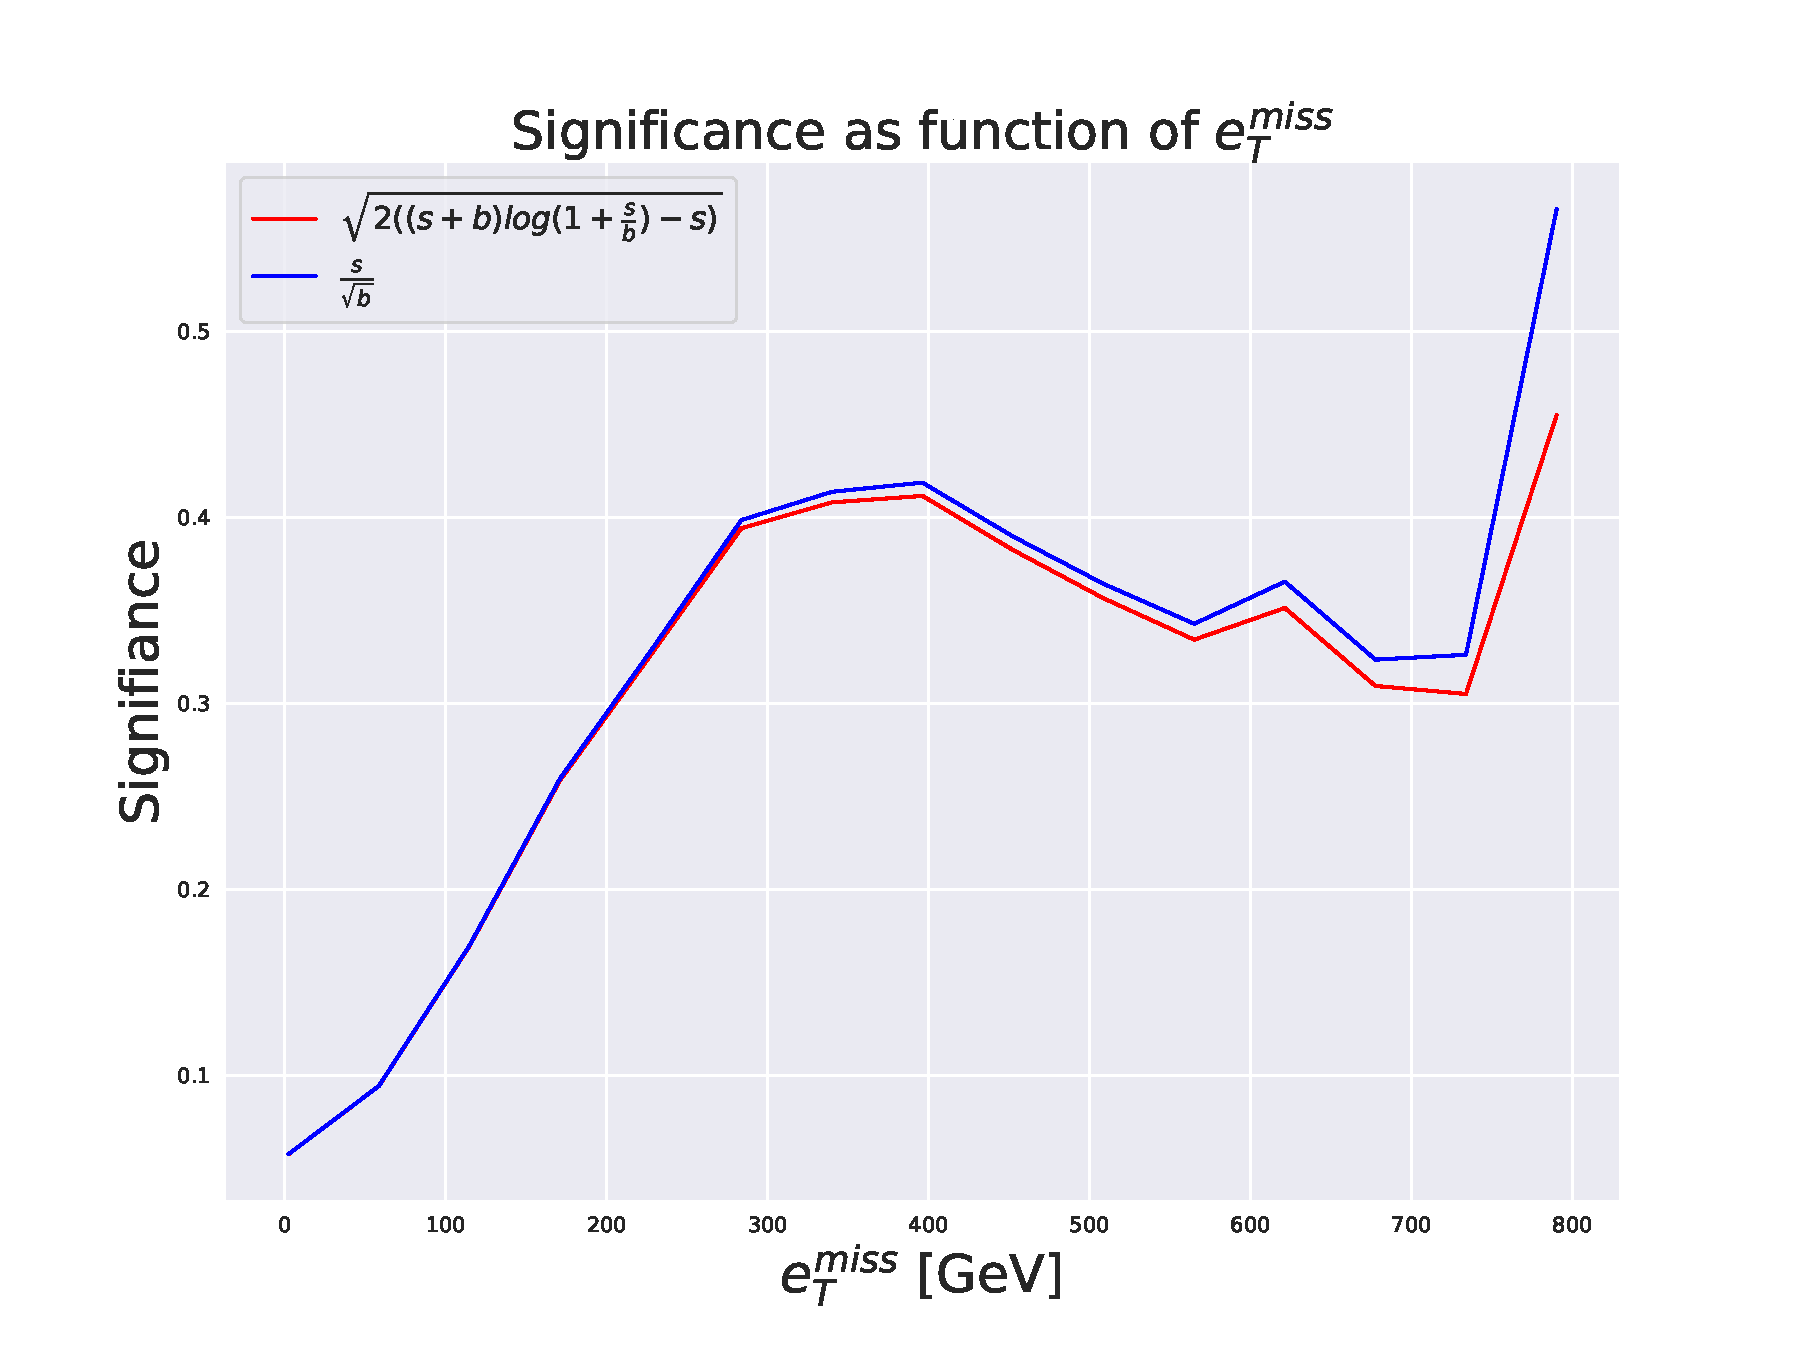
\includegraphics[width=\textwidth]{Figures/AE_testing/small/2lep/significance_etmiss_800p0p050_-1.6117055611472277.pdf}
        \caption{}
        \label{fig:AE_2lep_small_signi_800}
    \end{subfigure}
    \hfill      
    \caption[2lep shallow network | $800p50$ | AE]{Reconstruction error, $e_T^{miss}$ signal region, $m_{lll}$ signal region and significance as function of 
    $e_T^{miss}$ for the shallow regular autoencoder using SUSY $800p50$. In figures 
    \ref{fig:AE_2lep_small_800} there is a general trend here for both the small and large regular 
    autoencoder where the background distributions are highly shifted to the lower end of the 
    reconstruction error range. As the reconstruction error increases, the amount of each sample in a 
    given bin changes alot. In figure \ref{fig:AE_2lep_small_etmiss_800} there is a small separation 
    between the peaks of the background and the signal. There is still mostly overlap between the two distributions.}
    \label{fig:AE_2lep_small_rec_sig_signi_800}
\end{figure}


In figures \ref{fig:AE_2lep_big_rec_sig_signi_450}, \ref{fig:AE_2lep_small_rec_sig_signi_450}, 
\ref{fig:AE_2lep_big_rec_sig_signi_800} and \ref{fig:AE_2lep_small_rec_sig_signi_800} we have three 
subplots containing the total reconstruction error distributions, the $e_T^{miss}$ signal region, 
and the significance as function of $e_T^{miss}$ curve respectively. They were created using 
the shallow and deep regular autoencoder with the 2 lepton + $e_T^{miss}$ dataset.
In figures \ref{fig:AE_2lep_big_450}, \ref{fig:AE_2lep_small_450}, \ref{fig:AE_2lep_big_800}, 
\ref{fig:AE_2lep_small_800} there is a continuing trend following the 3 
lepton + $e_T^{miss}$ case shown in figures \ref{fig:AE_3lep_big_450}, \ref{fig:AE_3lep_small_450},
\ref{fig:AE_3lep_big_800}, \ref{fig:AE_3lep_small_800}. This indicates that as we increase the 
statistics, in other words the amount of background events 
used for training, the ability of the autoencoder to learn the internal structure increases. 
As expected, Zmmjets and Zeejets along with ttbar are the channels with the highest statistics 
in the 2 lepton + $e_T^{miss}$ dataset, thus it should be easier to learn to better reconstruct 
those events. However, note the amount of diboson in the higher end of the reconstruction error 
histograms, as well as in the $e_T^{miss}$ post reconstruction error cut distributions. 
Using the signal region definition \hl{from above} we set cuts on the reconstruction 
error and then calculate the significance of the signal. \par
In figures \ref{fig:AE_2lep_big_etmiss_450}, \ref{fig:AE_2lep_small_etmiss_450}, \ref{fig:AE_2lep_big_etmiss_800} and  
\ref{fig:AE_2lep_small_etmiss_800} we have the $e_T^{miss}$ distributions for 
the least strict cuts for the regular autoencoder models. One indication that the search strategy 
used in this thesis could work is if the models can improve the significance from just looking at 
the $e_T^{miss}$ distributions of the background and the signal in mind. Thus, we want to compare the pre 
reconstruction error significance with the signal region based on the autoencoder output. The significance 
in the pre reconstruction error case were for the SUSY $450p300$ signal 0.017 using both 
the small and large statistics formula, and 0.0014 for the SUSY $800p50$ signal. Note here that for 
$e_T^{miss}$, no physics informed cuts have been used, but there are certain cuts that can increase 
the significance, so the significance in should be considered to possibly be somewhat higher. \par
\par
In figures \ref{fig:AE_2lep_big_signi_450}, \ref{fig:AE_2lep_small_signi_450}, \ref{fig:AE_2lep_big_signi_800} 
and  \ref{fig:AE_2lep_small_signi_800} we have the significance as function of $e_T^{miss}$. From the 
function it 

\par

From figures \ref{fig:AE_2lep_big_signi_450}, \ref{fig:AE_2lep_small_signi_450}, \ref{fig:AE_2lep_big_signi_800} 
and  \ref{fig:AE_2lep_small_signi_800} we have the significance as a function of $e_T^{miss}$ for both signals 
using the shallow and deep autoencoder. This graph shows how implementing another cut in the signal region, 
namely where in the $e_T^{miss}$ distribution to select event, allows for higher significance. We see here 
that the shallow autoencoder gets a significance of almost 2.5 in the SUSY $450p300$ case, being the highest 
score, and beating the pre reconstruction error significance by alot. Another interesting point to note here 
is the tail ends, especially for the SUSY $800p50$ signal. This model has some events of very high $e_T^{miss}$, 
and in the tail end, there might be very few or none background events. It should be noted that the significance 
for the $800p50$ signal model is a lot smaller than for the $450p300$ signal model, even though the separation 
shown in figures \ref{fig:AE_2lep_big_450}, \ref{fig:AE_2lep_small_450}, \ref{fig:AE_2lep_big_800}, 
\ref{fig:AE_2lep_small_800} would suggest otherwise. Although the peak in both signal models are fairly 
separated from the peak of the SM MC, the SUSY $800p50$ signal model is shifted a lot more. This is 
consistent with expectation, for the same reason that the significance tails are the way they are.  Now, 
the reason for the low significance is most likely the fact that the signal sample contains low statistics, 
in other words, the weights are just a lot lower, compared to the other signal sample. \par

\subsubsection*{Variational autoencoder performance}

\begin{figure}[H]
    \centering
    \begin{subfigure}{.45\textwidth}
        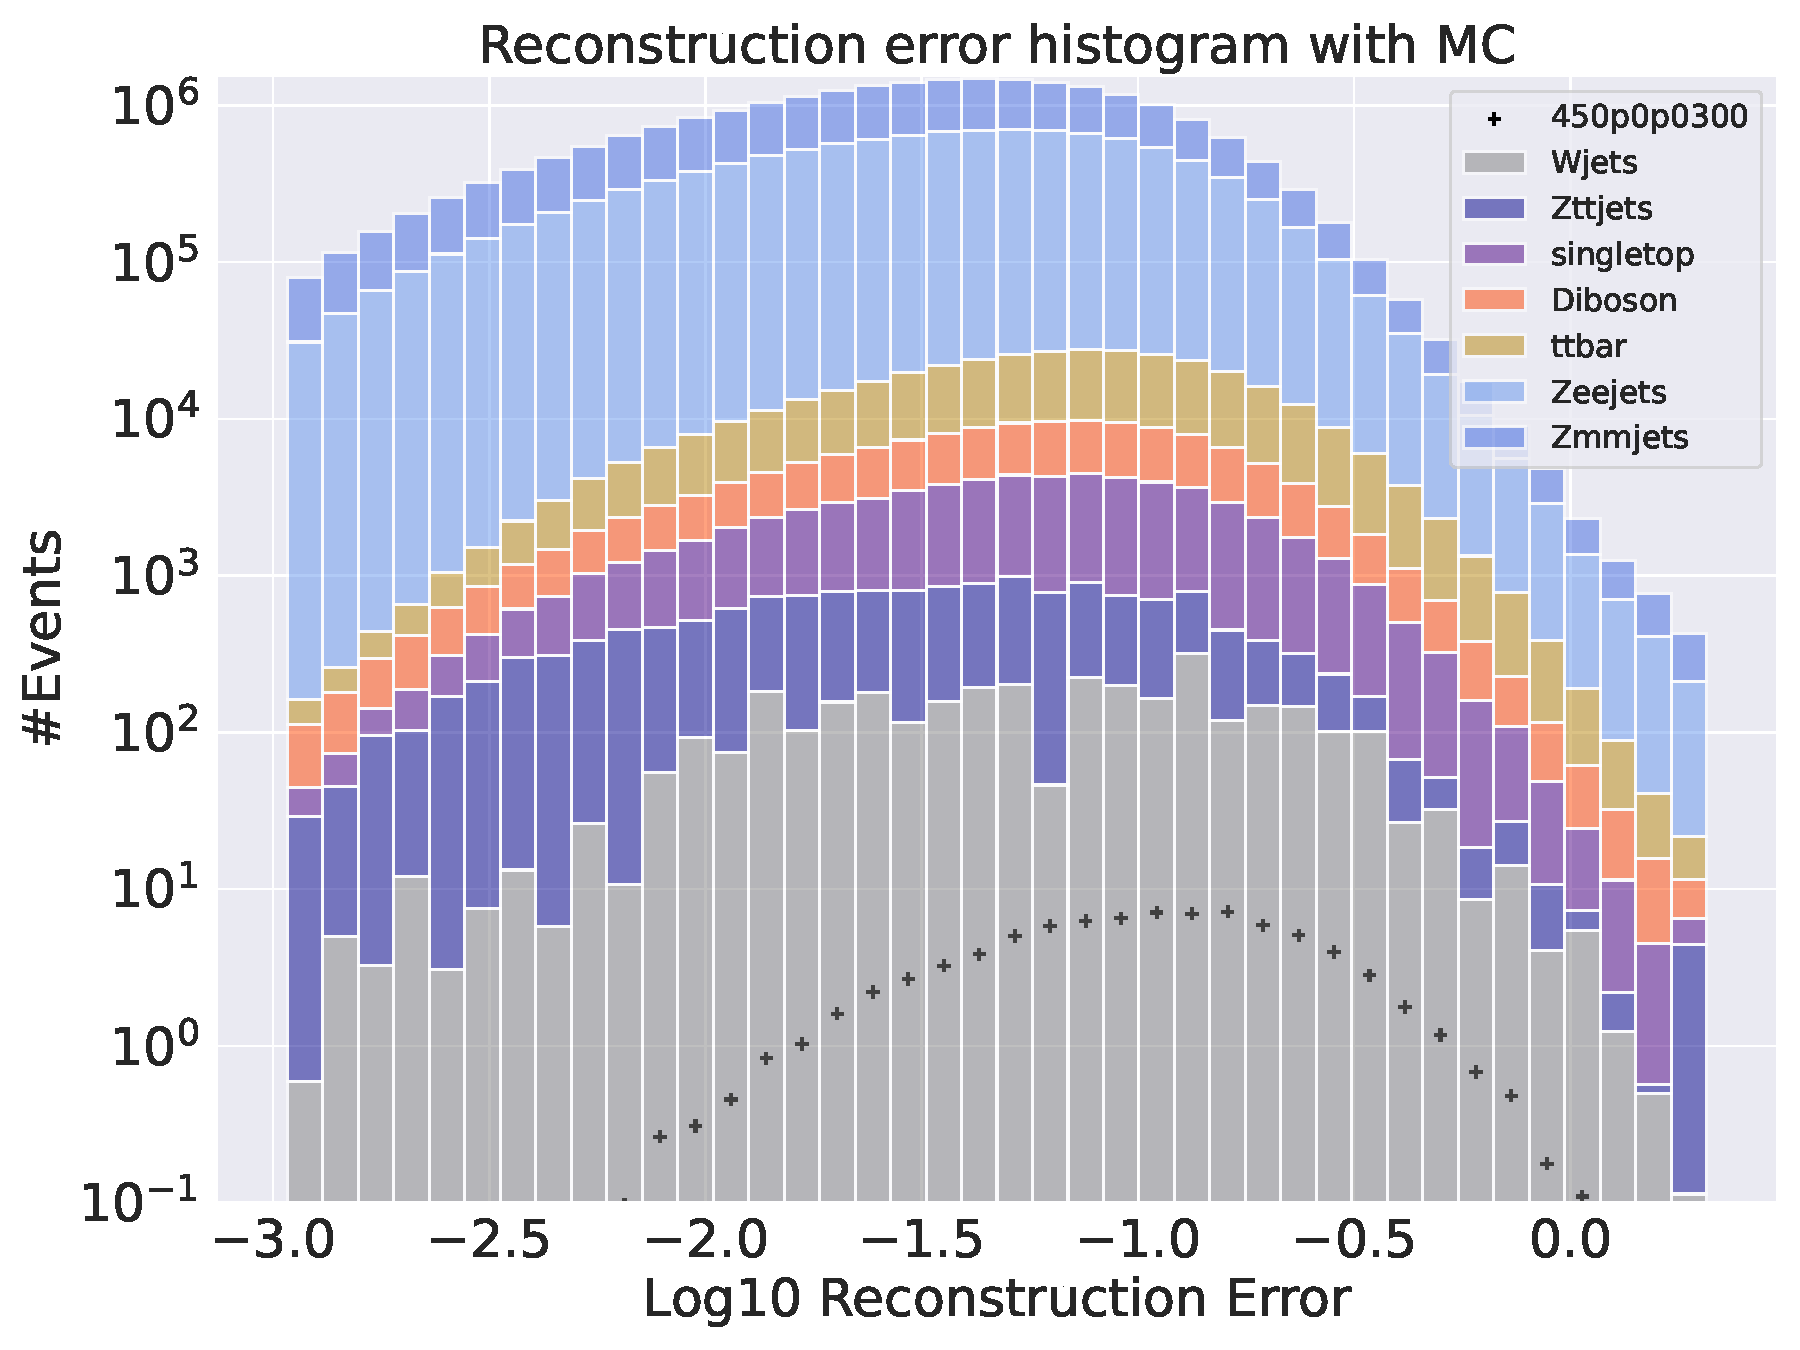
\includegraphics[width=\textwidth]{Figures/VAE_testing/small/2lep/b_data_recon_big_rm3_feats_sig_450p0p0300_.pdf}
        \caption{ }
        \label{fig:VAE_2lep_big_450}
    \end{subfigure}
    \hfill
    \begin{subfigure}{.45\textwidth}
        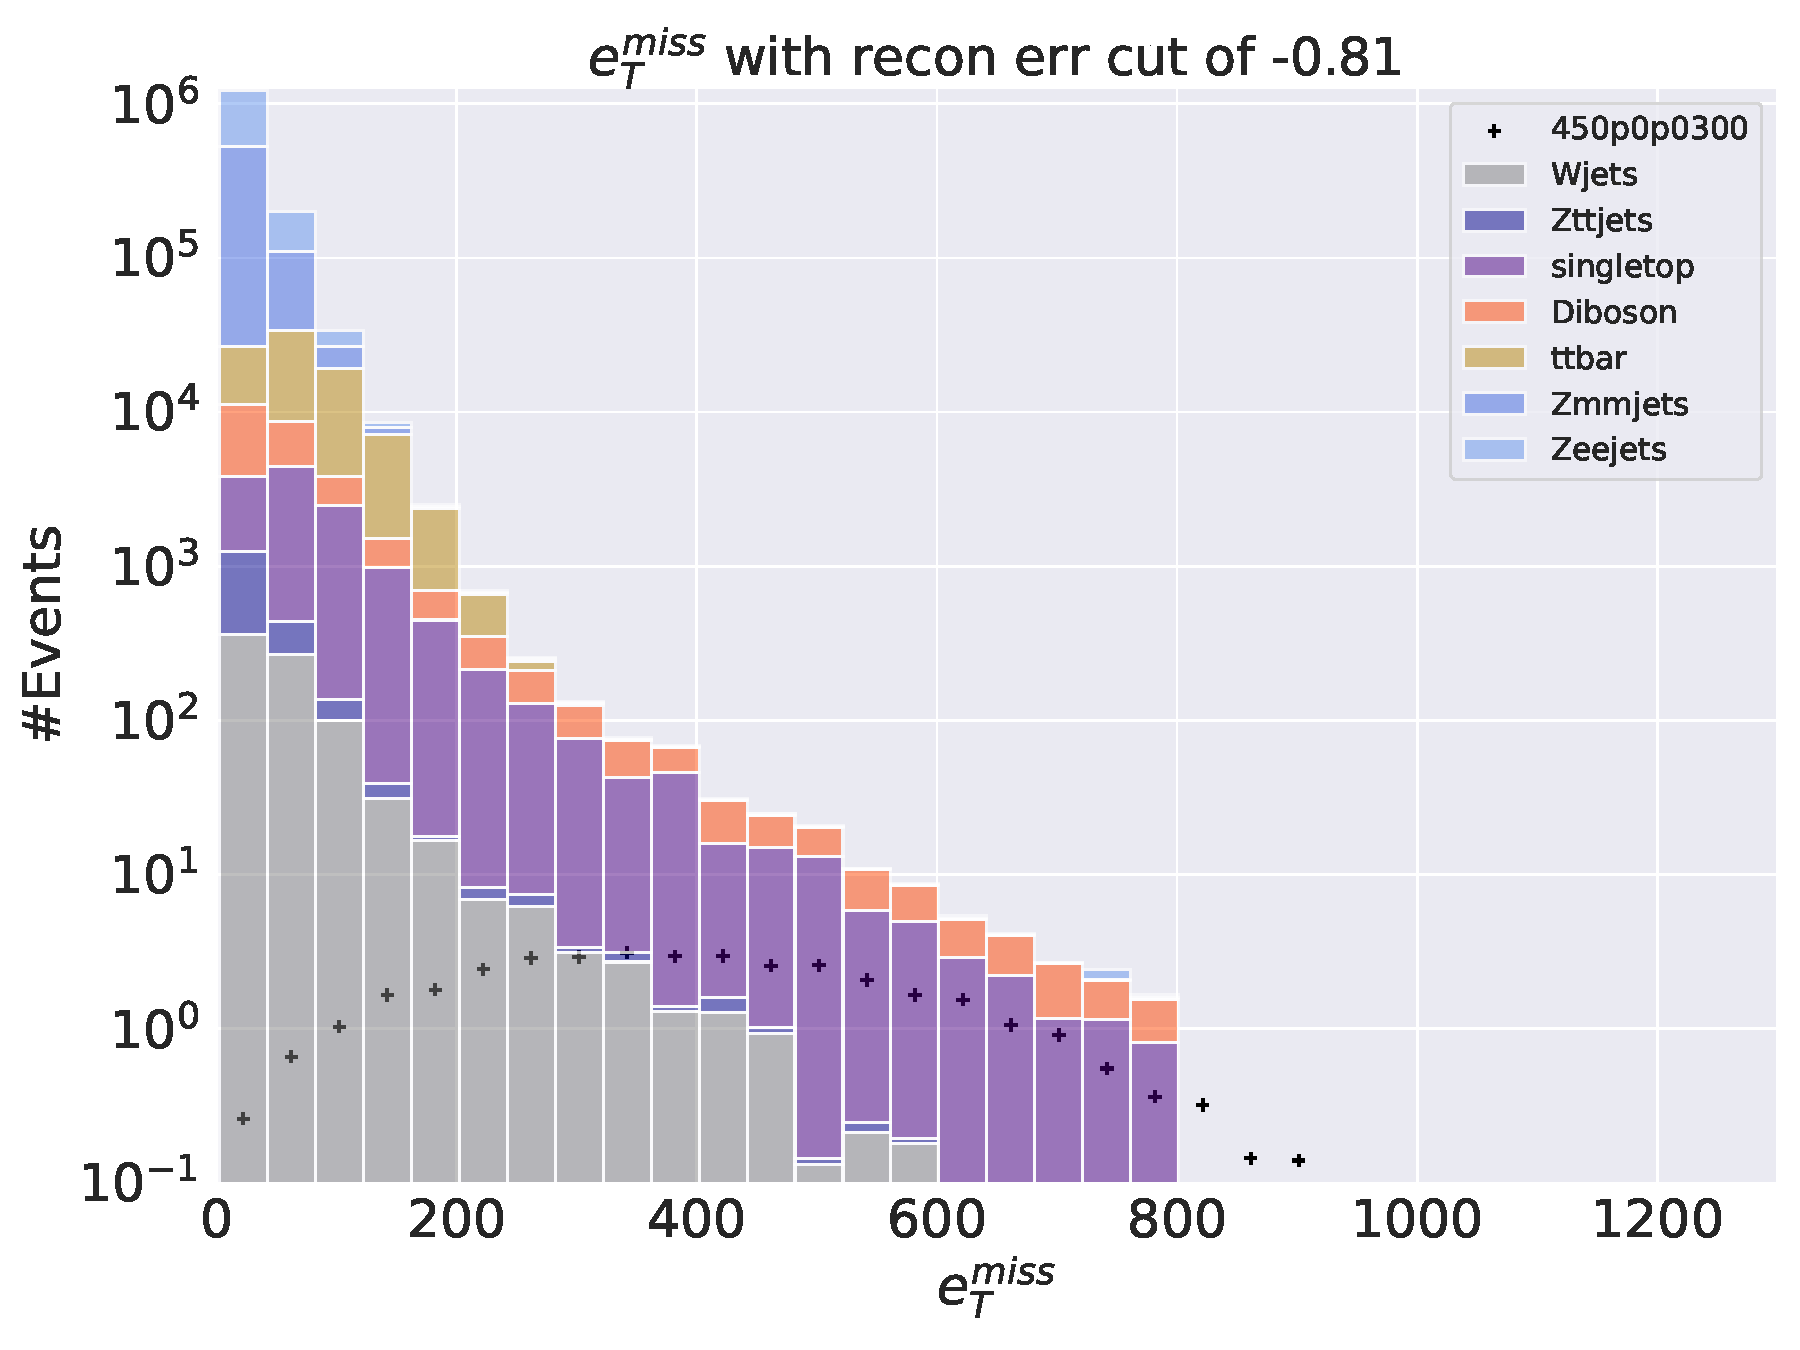
\includegraphics[width=\textwidth]{Figures/VAE_testing/big/2lep/b_data_recon_big_rm3_feats_sig_450p0p0300_recon_errcut_-0.81.pdf}
        \caption{}
        \label{fig:VAE_2lep_big_etmiss_450}
    \end{subfigure}
    \hfill 
    \begin{subfigure}{.45\textwidth}
        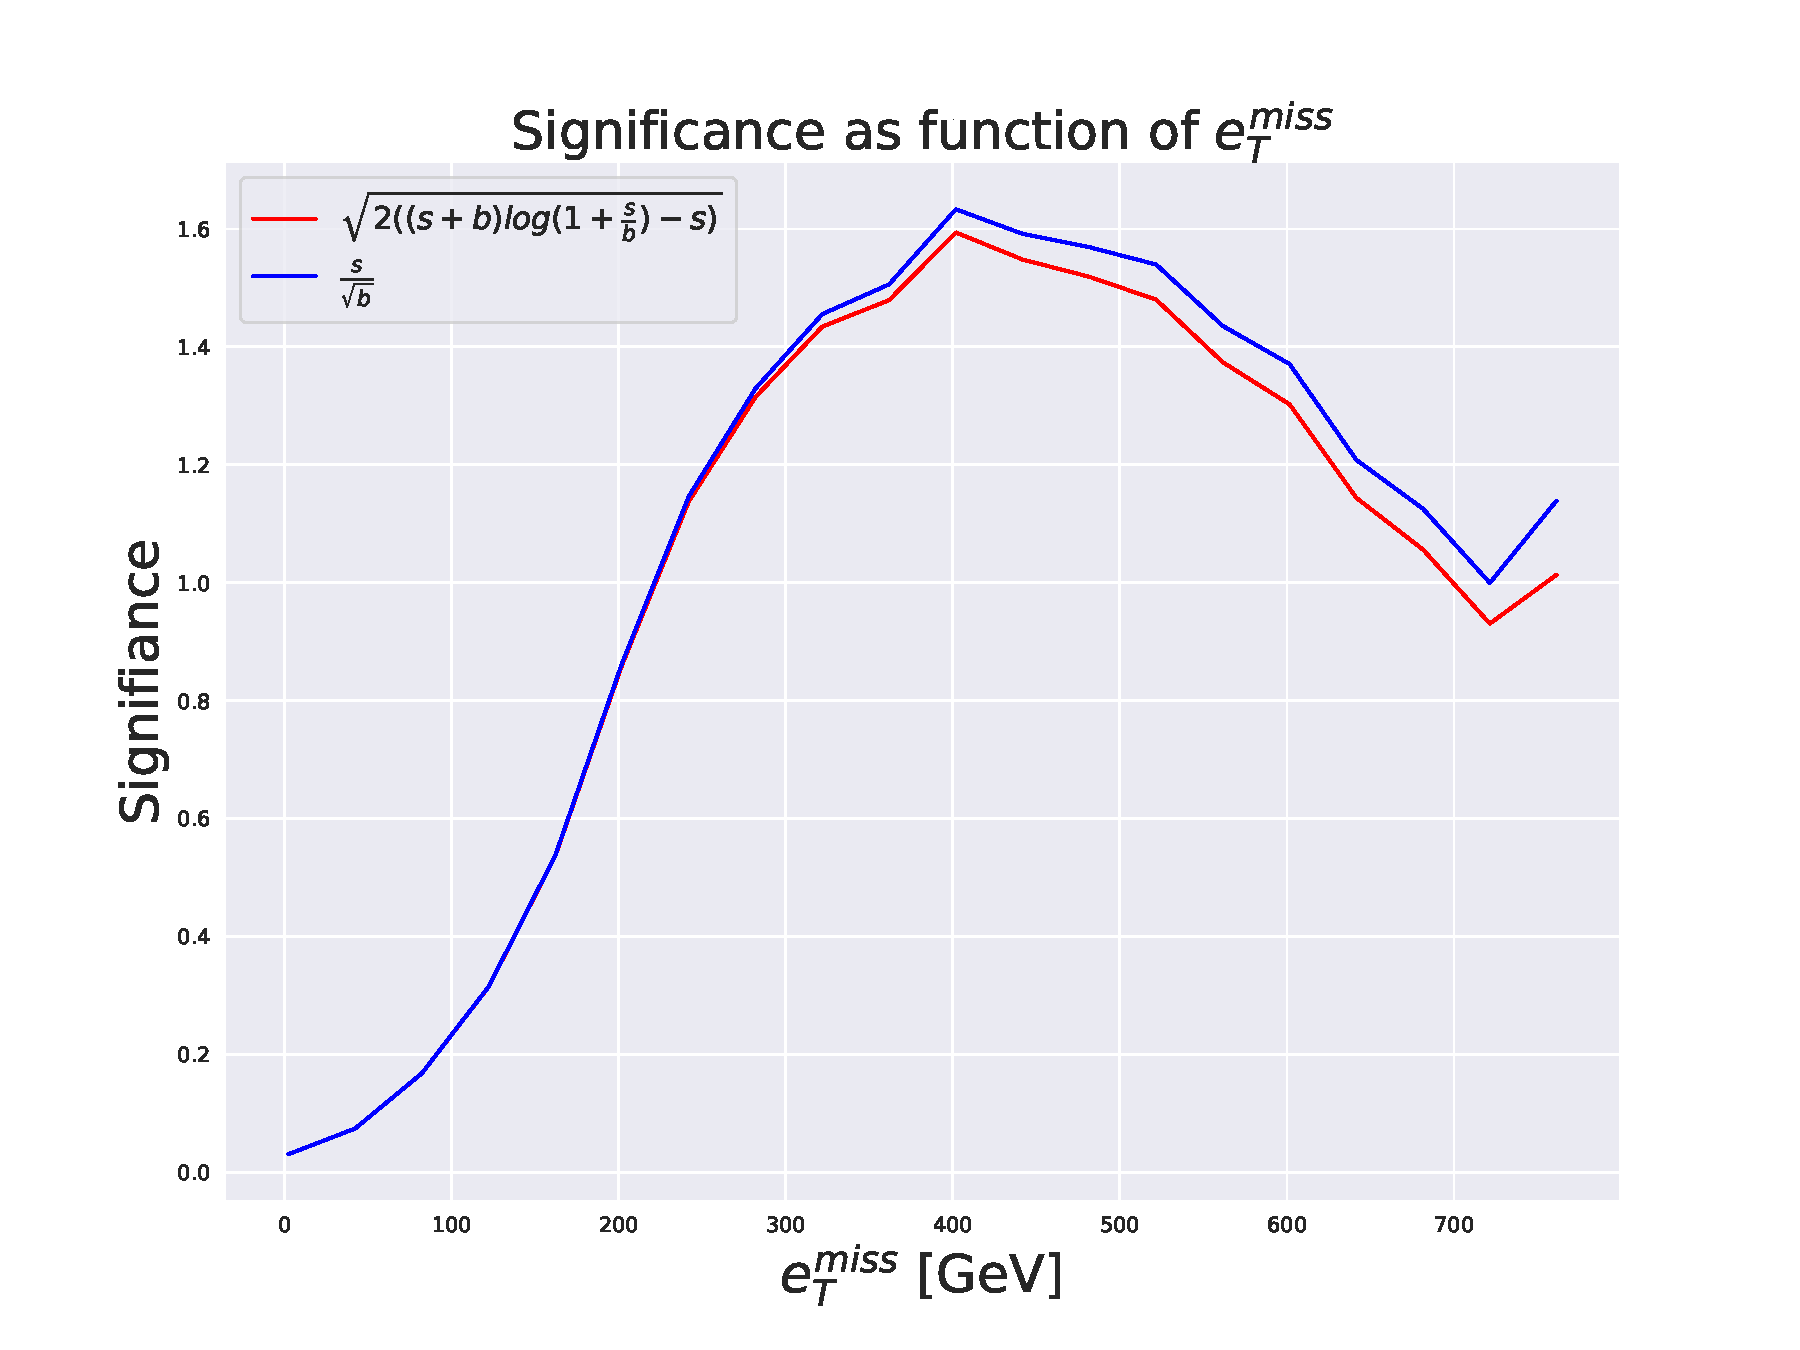
\includegraphics[width=\textwidth]{Figures/VAE_testing/big/2lep/significance_etmiss_450p0p0300_-0.8121874101107931.pdf}
        \caption{}
        \label{fig:VAE_2lep_big_signi_450}
    \end{subfigure}
    \hfill      
    \caption[2lep deep network | $450p300$ | VAE]{Reconstruction error, $e_T^{miss}$ signal region, $m_{lll}$ signal region and significance as function of 
    $e_T^{miss}$ for the deep regular autoencoder using SUSY $450p300$.}
    \label{fig:VAE_2lep_big_rec_sig_signi_450}
\end{figure}

\begin{figure}[H]
    \centering
    \begin{subfigure}{.45\textwidth}
        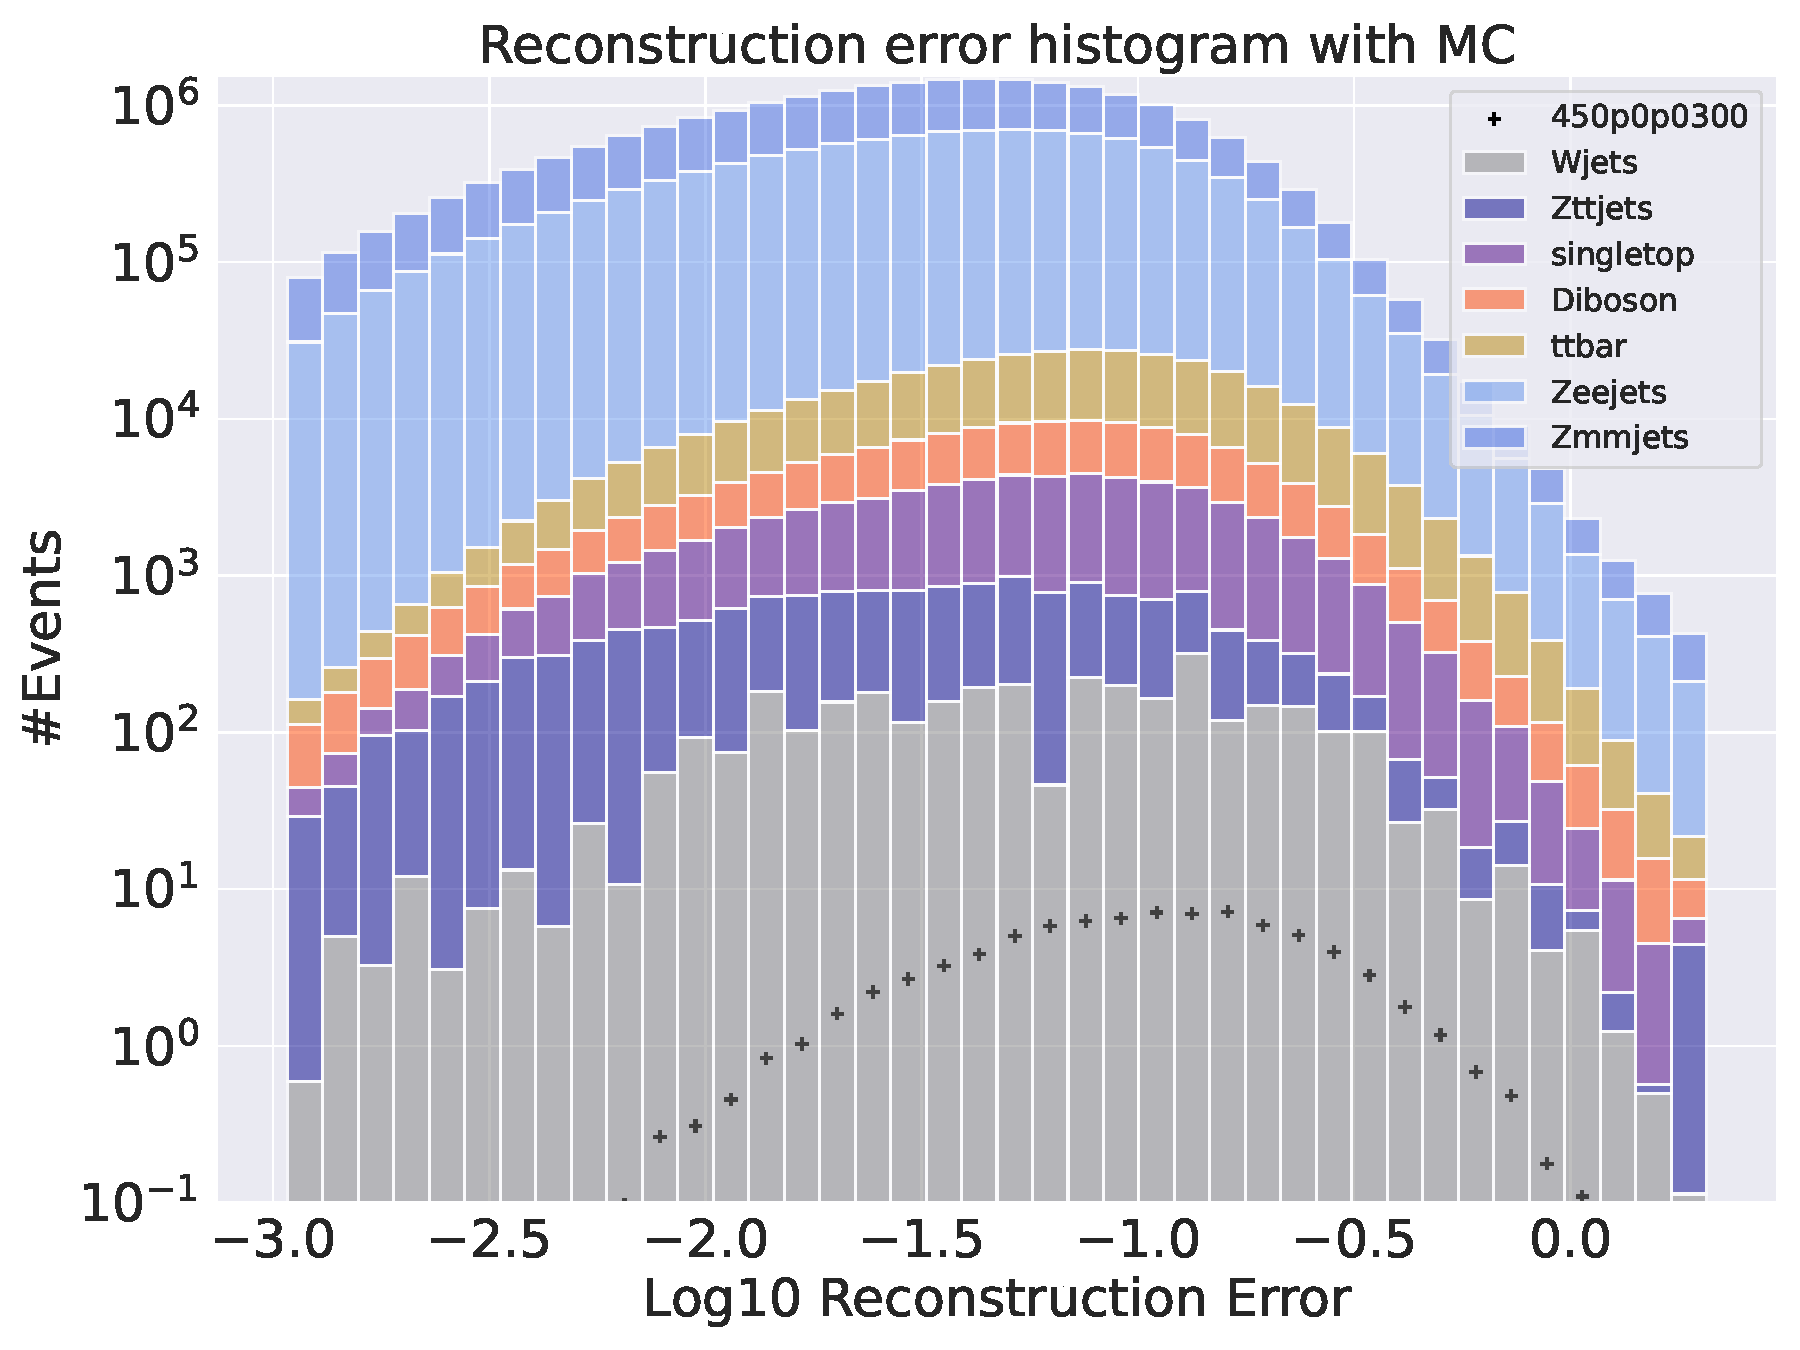
\includegraphics[width=\textwidth]{Figures/VAE_testing/small/2lep/b_data_recon_big_rm3_feats_sig_450p0p0300_.pdf}
        \caption{ }
        \label{fig:VAE_2lep_small_450}
    \end{subfigure}
    \hfill
    \begin{subfigure}{.45\textwidth}
        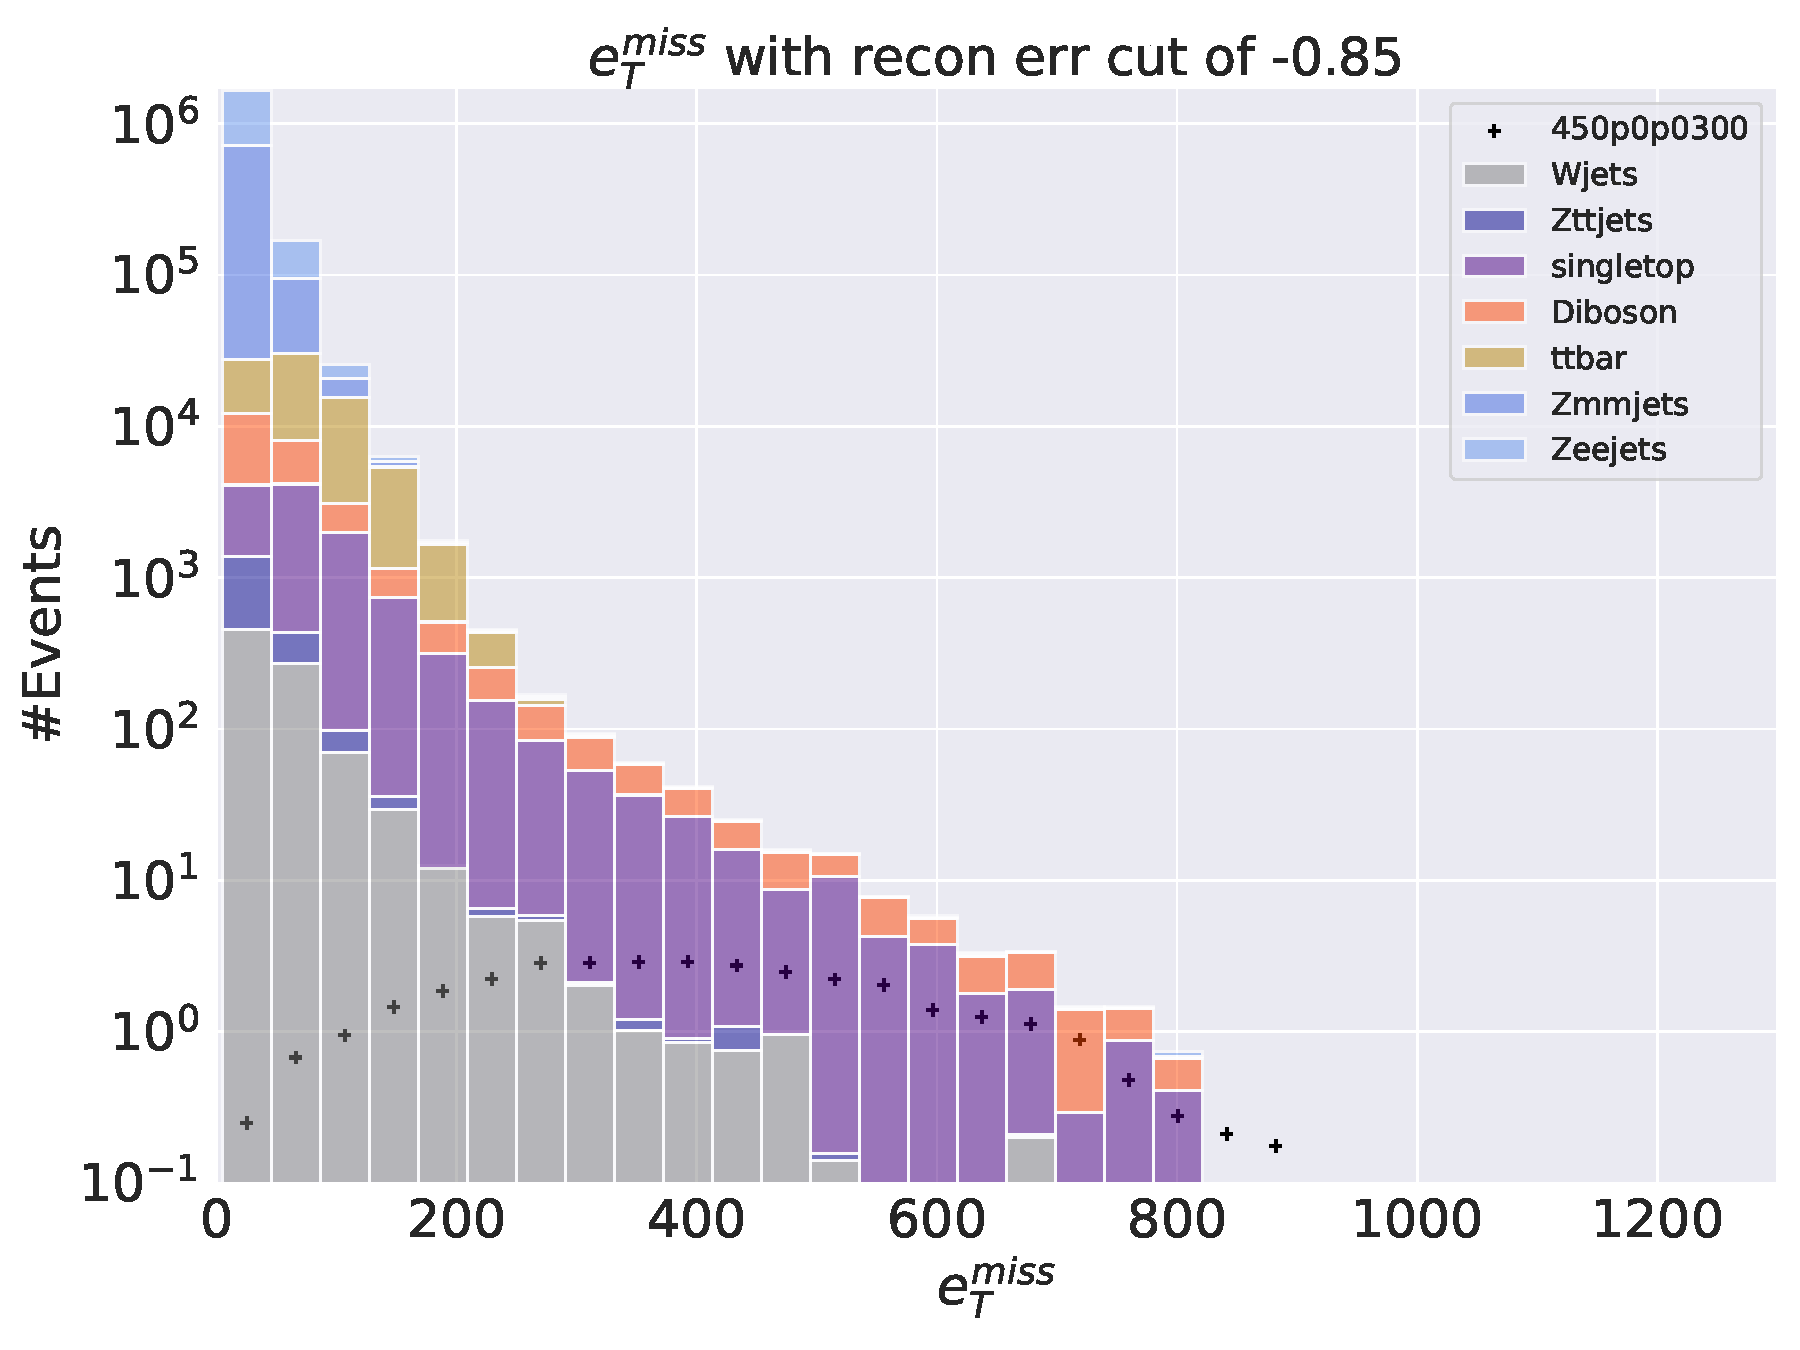
\includegraphics[width=\textwidth]{Figures/VAE_testing/small/2lep/b_data_recon_big_rm3_feats_sig_450p0p0300_recon_errcut_-0.85.pdf}
        \caption{}
        \label{fig:VAE_2lep_small_etmiss_450}
    \end{subfigure}
    \hfill  
    \begin{subfigure}{.45\textwidth}
        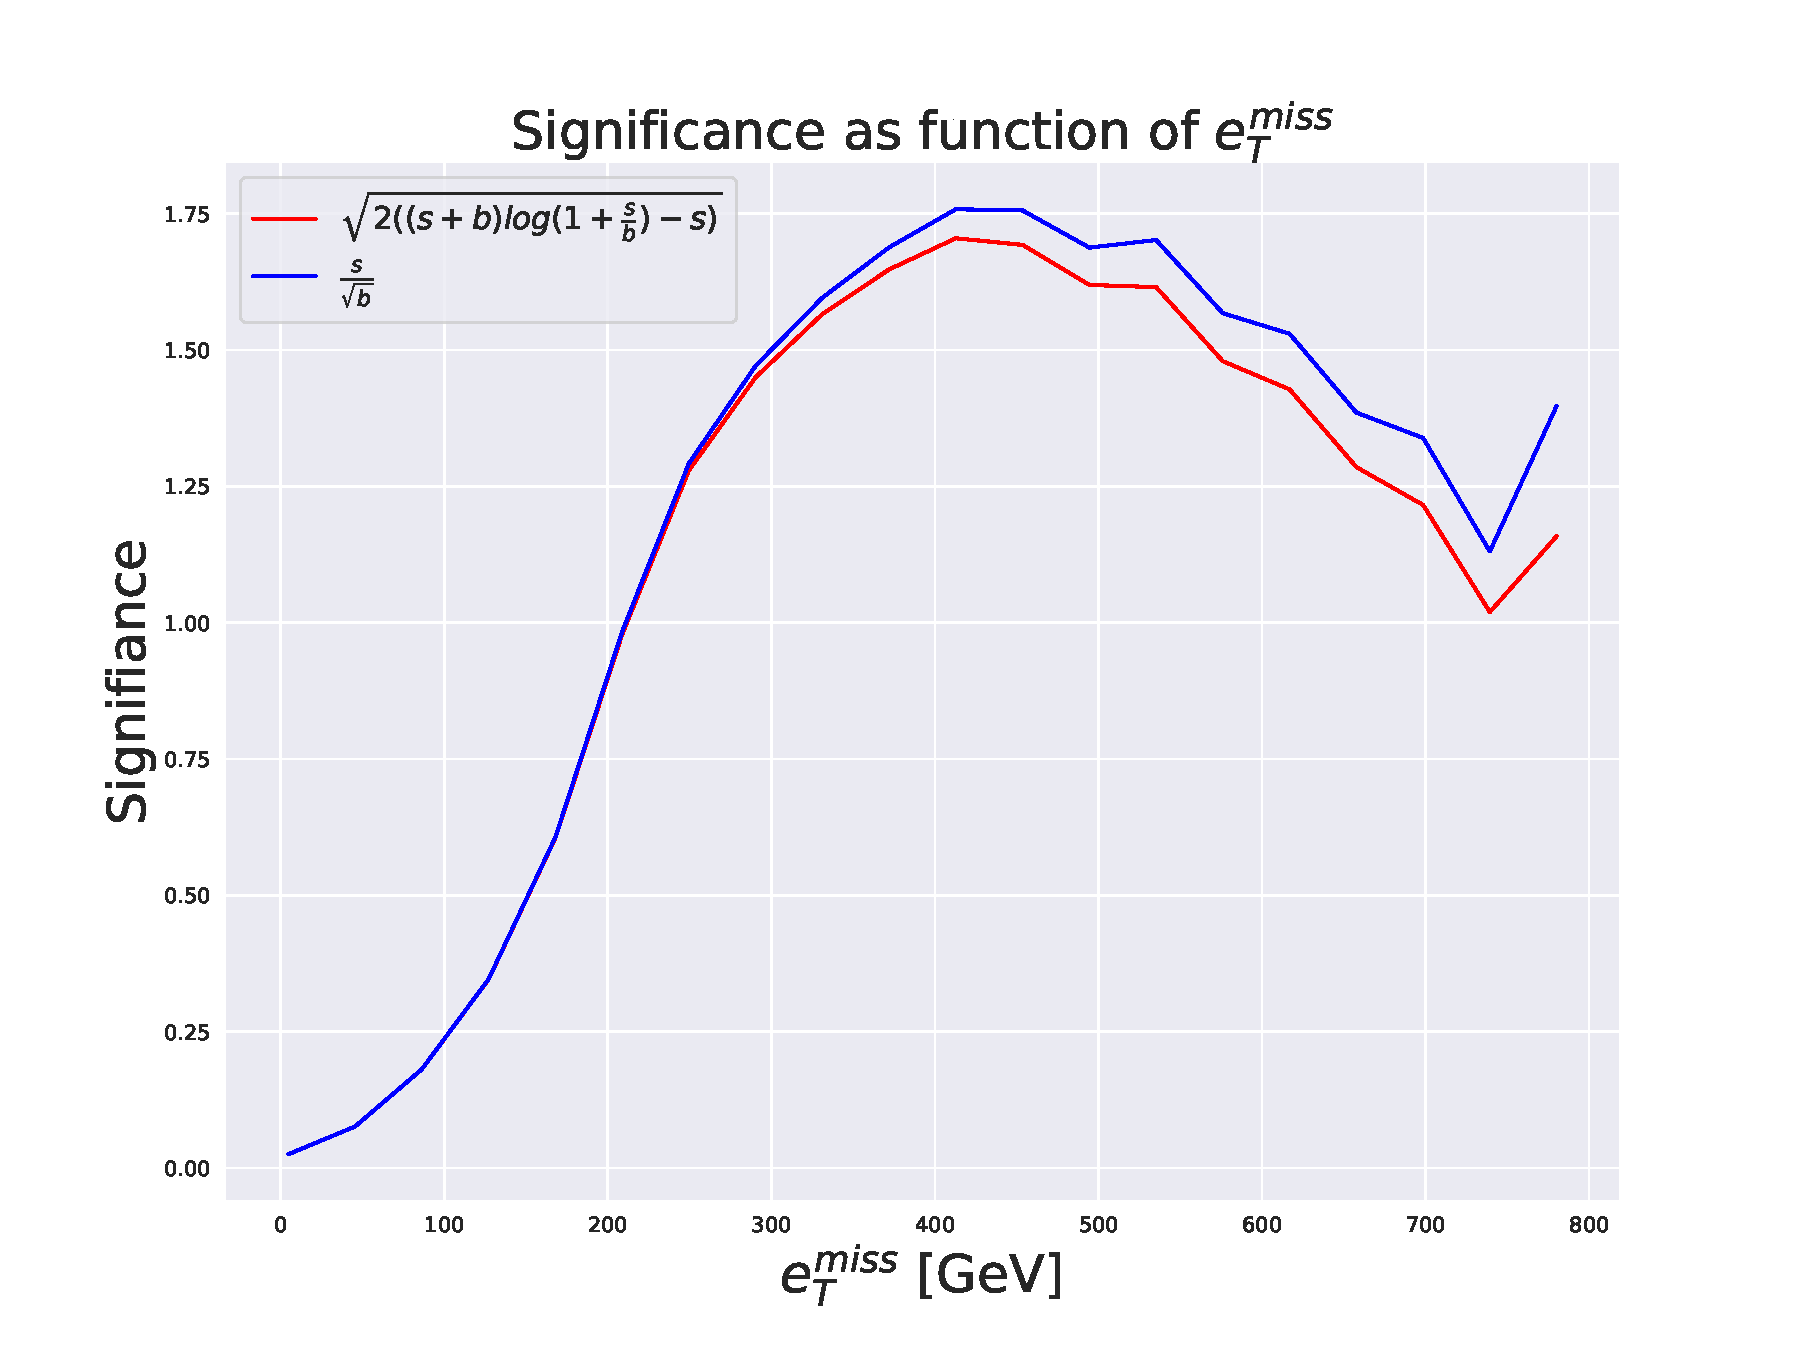
\includegraphics[width=\textwidth]{Figures/VAE_testing/small/2lep/significance_etmiss_450p0p0300_-0.8484803499636524.pdf}
        \caption{}
        \label{fig:VAE_2lep_small_signi_450}
    \end{subfigure}
    \hfill      
    \caption[2lep shallow network | $450p300$ | VAE]{Reconstruction error, $e_T^{miss}$ signal region, $m_{lll}$ signal region and significance as function of 
    $e_T^{miss}$ for the shallow regular autoencoder using SUSY $450p300$.}
    \label{fig:VAE_2lep_small_rec_sig_signi_450}
\end{figure}


\begin{figure}[H]
    \centering
    \begin{subfigure}{.45\textwidth}
        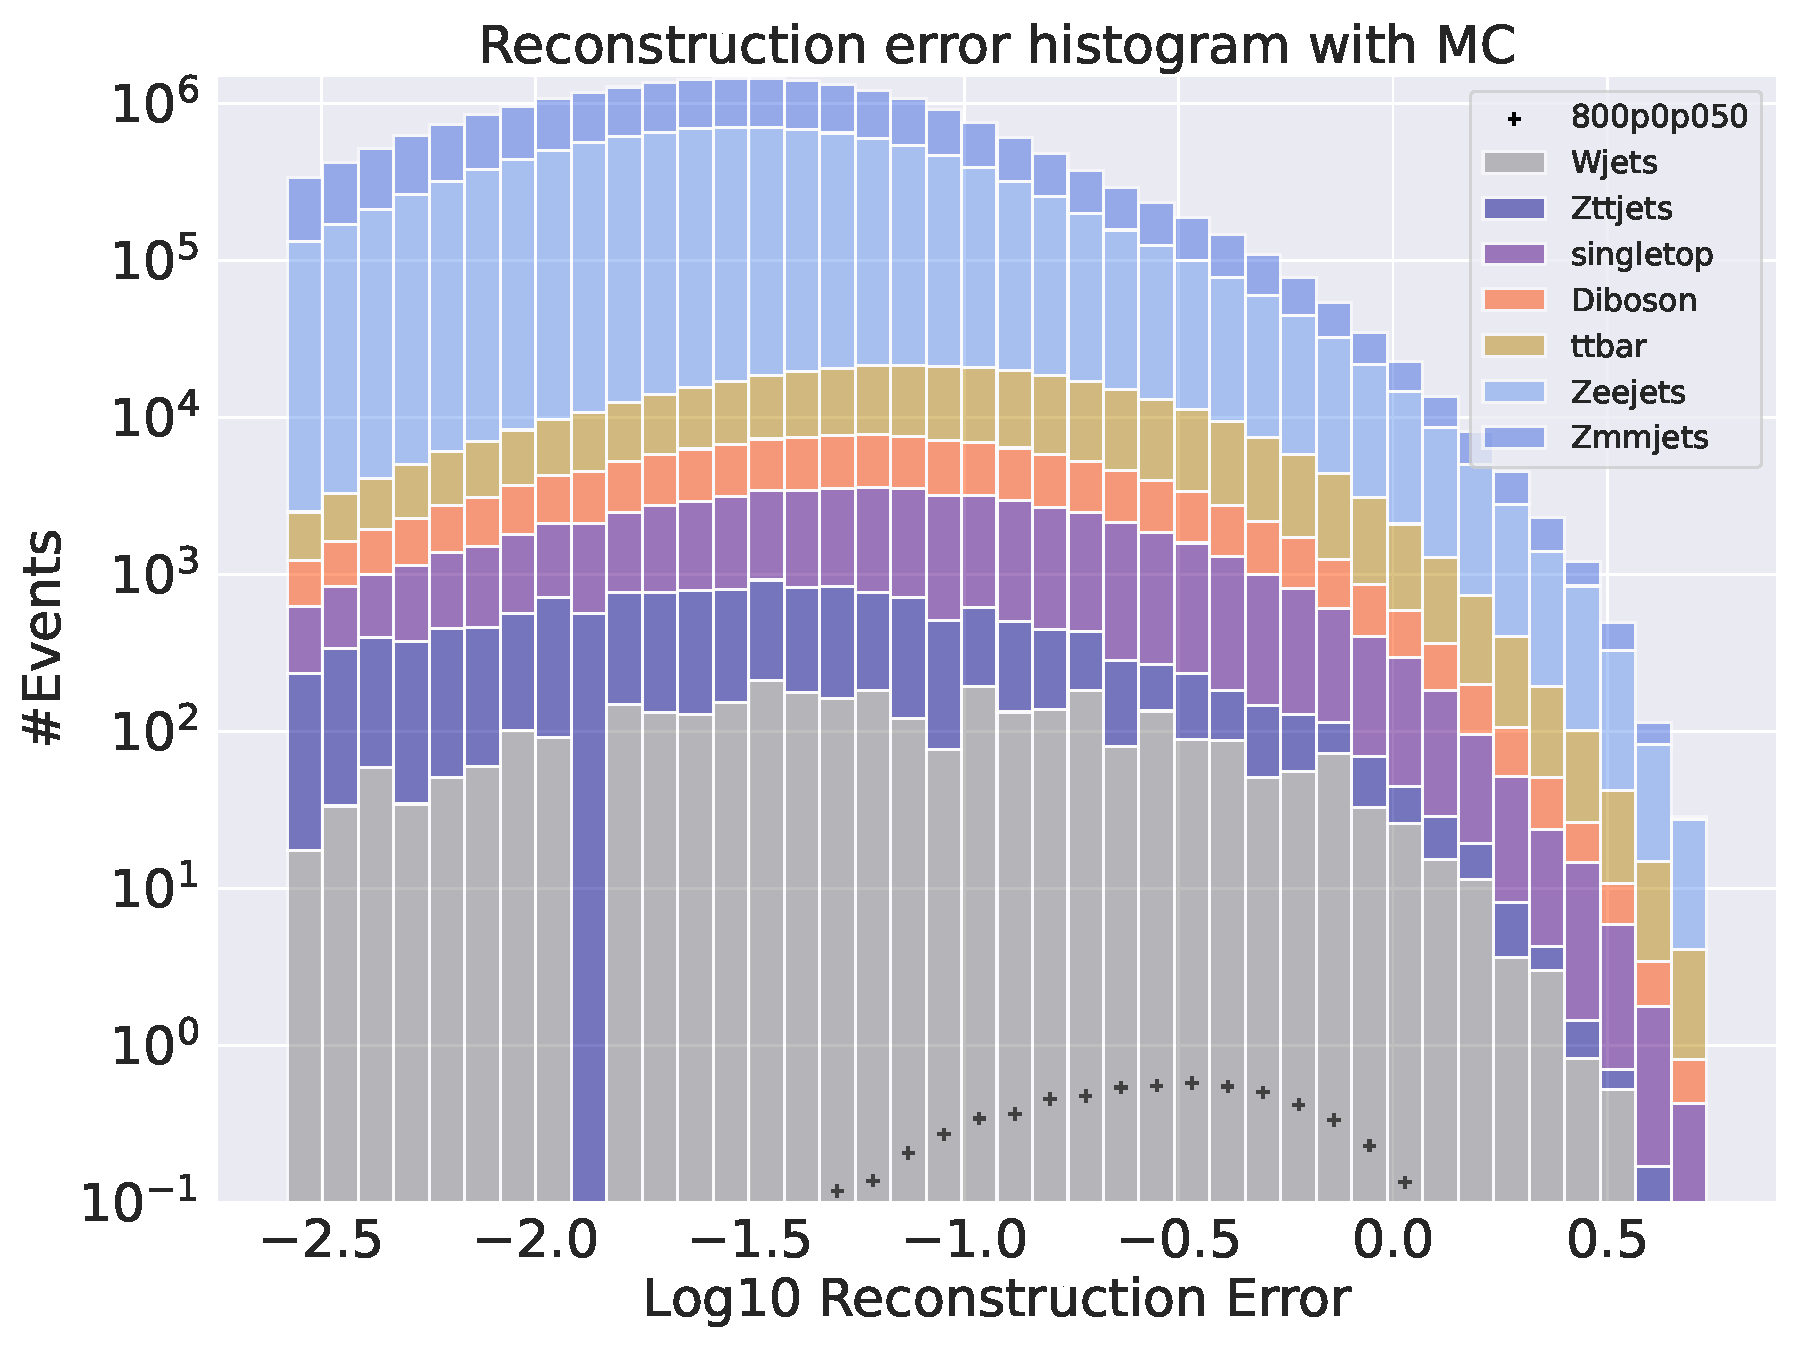
\includegraphics[width=\textwidth]{Figures/VAE_testing/big/2lep/b_data_recon_big_rm3_feats_sig_800p0p050_.pdf}
        \caption{ }
        \label{fig:VAE_2lep_big_800}
    \end{subfigure}
    \hfill
    \begin{subfigure}{.45\textwidth}
        \includegraphics[width=\textwidth]{Figures/VAE_testing/big/2lep/b_data_recon_big_rm3_feats_sig_800p0p050_recon_errcut_-0.72.pdf}
        \caption{}
        \label{fig:VAE_2lep_big_etmiss_800}
    \end{subfigure}
    \hfill
      
    \begin{subfigure}{.45\textwidth}
        \includegraphics[width=\textwidth]{Figures/VAE_testing/big/2lep/significance_etmiss_800p0p050_-0.7232197345309495.pdf}
        \caption{}
        \label{fig:VAE_2lep_big_signi_800}
    \end{subfigure}
    \hfill      
    \caption[2lep deep network | $800p50$ | VAE]{Reconstruction error, $e_T^{miss}$ signal region, $m_{lll}$ signal region and significance as function of 
    $e_T^{miss}$ for the deep variational autoencoder using SUSY $800p50$.}
    \label{fig:VAE_2lep_big_rec_sig_signi_800}
\end{figure}

\begin{figure}[H]
    \centering
    \begin{subfigure}{.45\textwidth}
        \includegraphics[width=\textwidth]{Figures/VAE_testing/small/2lep/b_data_recon_big_rm3_feats_sig_800p0p050_.pdf}
        \caption{ }
        \label{fig:VAE_2lep_small_800}
    \end{subfigure}
    \hfill
    \begin{subfigure}{.45\textwidth}
        \includegraphics[width=\textwidth]{Figures/VAE_testing/small/2lep/b_data_recon_big_rm3_feats_sig_800p0p050_recon_errcut_-0.85.pdf}
        \caption{}
        \label{fig:VAE_2lep_small_etmiss_800}
    \end{subfigure}
    \hfill  
    \begin{subfigure}{.45\textwidth}
        \includegraphics[width=\textwidth]{Figures/VAE_testing/small/2lep/significance_etmiss_800p0p050_-0.8542149600758421.pdf}
        \caption{}
        \label{ffig:VAE_2lep_small_signi_800}
    \end{subfigure}
    \hfill      
    \caption[2lep shallow network | $800p50$ | VAE]{Reconstruction error, $e_T^{miss}$ signal region, $m_{lll}$ signal region and significance as function of 
    $e_T^{miss}$ for the shallow variational autoencoder using SUSY $800p50$.}
    \label{fig:VAE_2lep_small_rec_sig_signi_800}
\end{figure}


In figures \ref{fig:VAE_2lep_big_rec_sig_signi_450}, \ref{fig:VAE_2lep_small_rec_sig_signi_450}, 
\ref{fig:VAE_2lep_big_rec_sig_signi_800} and \ref{fig:VAE_2lep_small_rec_sig_signi_800} we have three 
subplots containing the total reconstruction error distributions, the $e_T^{miss}$ signal region, 
and the significance as function of $e_T^{miss}$ curve respectively. They were created using 
the shallow and deep regular autoencoder with the 2 lepton + $e_T^{miss}$ dataset.
In figures \ref{fig:VAE_2lep_big_450}, \ref{fig:VAE_2lep_small_450}, \ref{fig:VAE_2lep_big_800}, 
\ref{fig:VAE_2lep_small_800} we have the reconstruction error distributions 
for both SUSY signals for the small and large variational autoencoder. Here we observe that the 
peak of the distributions for the SM MC in all four cases are somewhat centered in the middle 
of the reconstruction error range, which differs from the steep slope we saw in figures 
\ref{fig:AE_2lep_big_450}, \ref{fig:AE_2lep_small_450}, \ref{fig:AE_2lep_big_800}, 
\ref{fig:AE_2lep_small_800}. Interestingly, we see here that the deepness of the neural 
network here plays a role, which is different from the regular autoencoder output, where both 
the small and large autoencoder made a steep slope shape of the SM MC reconstruction error 
distribution. The peak of the distribution here is slightly shifted to the left for the shallow 
autoencoder model, and slightly shifted to the right of the center with the deep autoencoder 
model. One possible reason for this somewhat Gaussian like distribution could be that the 
variational autoencoder, via the reparametization trick from section \ref{sec:reparameterization}, 
samples from a Gaussian distribution that has yet to be trained on enough data to produce a 
good enough error distribution. This is also supported with the fact that the shape is even more 
Gaussian like in the 3 lepton + $e_T^{miss}$ case shown in figures \ref{fig:VAE_3lep_big_450}, 
\ref{fig:VAE_3lep_small_450}, \ref{fig:VAE_3lep_big_800}, \ref{fig:VAE_3lep_small_800}. 
It could also be that the batch size is too large, and that the model has to train on smaller 
batches to get a better result. \par 

In figures \ref{fig:VAE_2lep_big_etmiss_450}, \ref{fig:VAE_2lep_small_etmiss_450}, 
\ref{fig:VAE_2lep_big_etmiss_800} and  \ref{fig:VAE_2lep_small_etmiss_800} we have 
the $e_T^{miss}$ distribution for the least strict cut for each signal. We see that 
the cuts are somewhat similar to the regular autoencoder, but with two key differences.
First, because the peaks of the distributions from figures \ref{fig:VAE_2lep_big_450}, 
\ref{fig:VAE_2lep_small_450}, \ref{fig:VAE_2lep_big_800}, \ref{fig:VAE_2lep_small_800} 
are so close, the cuts allowed for more background events in the signal region. Here, 
as with the regular autoencoder output, $m_{err}$ was used, but was not a good descriminator 
for the background events. One could perhaps make a new strategy for setting the cuts in 
the event one has a "fat gaussian" shape. Still, because we set cuts based on reconstruction 
error to mimimize the background in the signal region, if one does not have a slope like shape, 
the results will be poor in comparison. \par 
Secondly, the background that remains are slightly 
different from the signal region from the regular autoencoder. In the lower energy range there 
is a large excess of Zeejets, Zmmjets and ttbar events that have a high reconstruction error, 
which is not the case for the variational autoencoder, dominated by diboson events in all bins. 
In the higher energy range, diboson are largest contributer to the background, but the number 
of bins are exceptionally smaller than the Zmmjets/Zeejets/ttbar events, by a magnitude of 3 at the most. 


 
\section{Challenges with the search method and tools}

In the previous sections, the output and results of using the autoencoder for anomaly detection have been shown. 
The method and results, as produced and shown in this thesis, have yielded some promising results, given the nature 
of the search method. However, it should be known what the challenges of the task actually are, to truly understand 
why the results only are promising, and not great compared to other search methods. The challenges can be divided into 
three main points, all of which are entangled together. The three challenges are listed below. 

\begin{itemize}
    \item Model independence
    \item Reconstruction error minimization
    \item Feature engineering
\end{itemize}

Model independence is the first challenge. By model it is here referring to signal models, which it self might be self 
explanatory, but is a incredibly difficult criteria to uphold. As mentioned in the theory section for the Standard Model, 
the Standard Model, all though very successful in certain predictions, lack the ability to explain a whole number of 
behavior around us, and so there have been made a large numbers of suggested solutions to the issues. These new models are 
often called extensions to the Standard Model, and all though mathematically consistent, not neccesarly physically possible. 
And even if they are physically possible, in other words, they adhere to certain fundamental physical principles, they 
still might not exsist, as several searches at ATLAS have exluded but never found any new physics. The search method is inherently 
biased as one assumes that the new physics looks like the signal, and thus do analysis, data preparation etc with that 
signal in mind. But we do not know, at all, what the new physics looks like, even the assumption that we are looking for 
particles are implying a bias that might not be true. From the collisions in the detector to the analysis, there are biased descisions, 
we cannot avoid them, but we can minimize them as much as possible, which is a goal with the search strategy in this thesis. \par
This leads us to the second challenge, which is reconstruction error minimization. The proposed method in this thesis is to 
learn the signature of the standard model so well, that even subtle anomalous behavior will be picked up by the analysis tool. 
The autoencoder learns the signature of the standard model, by mimimizing the reconstruction error, and then hopefully, the 
anomalous data will be picked up and skewed to the right end of the reconstructino error distribution in a signal region. 
One problem with this is that one first blinds oneself to signals that might be very, very similar to the standard model in some 
feature space, but with very low statistics. These events will for a given set of features, never be found. \par 
The The third challenge is the choice of features. This thesis utilized the RMM structure by Chekanov et al, as it maximizes 
the amount of information in the input data by using almost completely uncorrolated features. However, as we do not know the signals 
we are looking for, there is no way to know if this choice is the optimal choice for new physics. In fact, even if we found 
an ideal set of features, based on some physical principles or something else, it is not trivial that the reconstruction error calculation
should weight the error of each feature equally. It might very well be that some features are less important than others. Essentially, 
the goal is to optimize for a signal we do not know, using features we dont know are optimal, and weighting them as "unbiased" as 
possible, simply taking the average, to dictate how the autoencoder learns and updates its internal weights and biases. 



%%%%%%%%%%%%% Conclusion %%%%%%%%%%%%%%%%%%%%%%%%%%
\chapter{Conclusion}
\addcontentsline{toc}{chapter}{Conclusion} 

%\medskip

The main goal of this thesis was to benchmark and investigate the performance and usage of
autoencoders in BSM searches. The analysis and testing were done using 
n-tuples from ATLAS that was converted to python dataframe structures. We argued for using 
the Rapidity-Mass matrix as features in our input data, with 6 bjets and 6 ljets, and 6 
of each lepton. The original goal was to test and understand the performance in the case
where we have a 3 lepton + $e_T^{miss}$ final state. In testing, it was shown that the 
performance was not too impressive, thus the choice was made to use the 2 lepton + $e_T^{miss}$ dataset which 
contains much more data. Due to the large size of the total dataset, we proposed a solution
where the overall distribution in the total set was conserved in smaller batches, called 
megasets. Several tests were deviced to benchmark the autoencoders, 
making anomalous events by altering the $p_T$ of standard model events and testing on two 
supersymmetric signal models. We showed that the autoencoders performance increased with 
larger training samples, but argue for more testing as these methods are not well 
understood yet. The performance was measured in three categories: how well it reconstructs 
the test dataset; how much background and signal is left in the signal region; and 
the significance it achieves when performing cuts in the signal region. It was shown that
for the first category, the regular autoencoder is much better than the variational autoencoder, 
creating a reconstruction error distribution with slope like shape pushed to the lower end. 
In the second category the regular autoencoder is much better at 
reducing the background, but not that much better at increasing the amount of signal. In the 
third category the regular autoencoder performs better than the variational autoencoder. 
It was also shown that with an increase in training data, the first category was improved 
for both the regular autoencoder and the variational autoencoder. \par 
We also argue for future work and challenges with the method. Amongst other 
issues where computational bottlenecks related to writing and loading of data from training 
and inference. It is recommended to further investigate the RMM, as well as alter 
the training process by physics informed or machine learning informed choices, such as a 
weighted MSE. 
\backmatter{}


%%%%%%%%%%%%% Appendix %%%%%%%%%%%%%%%%%%%%%%%%

\begin{appendices}
\numberwithin{equation}{section}

\appendix
\chapter{Appendix A}
\renewcommand{\thechapter}{A}
\renewcommand{\theequation}{\thechapter.\arabic{equation}}
\section{Algorithmic implementation}\label{sec:algo_impl}

The RMM as a set of features were a bit tricky to implement, and one way to implement it was 
to use a dictionary containing the names of features already in the RDataFrame set. RDataFrame 
allows for custom c++ functions to be run on the entire dataframe, and because almost all the 
features in the RMM use the kinematical variables for each particle they were needed to 
be accessed. Each element in the dictionary contains a number ID corresponding to the column 
it belongs to, a name, the 4 kinematic variables $p_T$, $\eta$, $\phi$ and E, and the rank 
within its particle type. Thus, $ele_0$ is the first electron, and its rank is 0. 

\begin{lstlisting}[language=Python, style=pythonstyle, label={code:rmm_dict_struct}]
rmm_structure = {
    1: ["ljet_0", "jetPt[ljet]", "jetEta[ljet]", "jetPhi[ljet]", "jetM[ljet]", 0,],
    2: [ "ljet_1", "jetPt[ljet]", "jetEta[ljet]", "jetPhi[ljet]", "jetM[ljet]", 1,],
    3: [ "ljet_2", "jetPt[ljet]", "jetEta[ljet]", "jetPhi[ljet]", "jetM[ljet]", 2,],
    4: [ "ljet_3", "jetPt[ljet]", "jetEta[ljet]", "jetPhi[ljet]", "jetM[ljet]", 3,],
    5: [ "ljet_4", "jetPt[ljet]", "jetEta[ljet]", "jetPhi[ljet]", "jetM[ljet]", 4,],
    6: [ "ljet_5", "jetPt[ljet]", "jetEta[ljet]", "jetPhi[ljet]", "jetM[ljet]", 5,],
    7: [ "bjet_0", "jetPt[bjet77]", "jetEta[bjet77]", "jetPhi[bjet77]", "jetM[bjet77]", 0,],
    8: [ "bjet_1", "jetPt[bjet77]", "jetEta[bjet77]", "jetPhi[bjet77]", "jetM[bjet77]", 1,],
    9: [ "bjet_2", "jetPt[bjet77]", "jetEta[bjet77]", "jetPhi[bjet77]", "jetM[bjet77]", 2,],
    10: [ "bjet_3", "jetPt[bjet77]", "jetEta[bjet77]", "jetPhi[bjet77]", "jetM[bjet77]", 3,],
    11: [ "bjet_4", "jetPt[bjet77]", "jetEta[bjet77]", "jetPhi[bjet77]", "jetM[bjet77]", 4,],
    12: [ "bjet_5", "jetPt[bjet77]", "jetEta[bjet77]", "jetPhi[bjet77]", "jetM[bjet77]", 5,],
    13: [ "ele_0", "lepPt[ele_SG]", "lepEta[ele_SG]", "lepPhi[ele_SG]", "lepM[ele_SG]", 0,],
    14: [ "ele_1", "lepPt[ele_SG]", "lepEta[ele_SG]", "lepPhi[ele_SG]", "lepM[ele_SG]", 1,],
    15: [ "ele_2", "lepPt[ele_SG]", "lepEta[ele_SG]", "lepPhi[ele_SG]", "lepM[ele_SG]", 2,],
    16: [ "ele_3", "lepPt[ele_SG]", "lepEta[ele_SG]", "lepPhi[ele_SG]", "lepM[ele_SG]", 3,],
    17: [ "ele_4", "lepPt[ele_SG]", "lepEta[ele_SG]", "lepPhi[ele_SG]", "lepM[ele_SG]", 4,],
    18: [ "muo_0", "lepPt[muo_SG]", "lepEta[muo_SG]", "lepPhi[muo_SG]", "lepM[muo_SG]", 0,],
    19: [ "muo_1", "lepPt[muo_SG]", "lepEta[muo_SG]", "lepPhi[muo_SG]", "lepM[muo_SG]", 1,],
    20: [ "muo_2", "lepPt[muo_SG]", "lepEta[muo_SG]", "lepPhi[muo_SG]", "lepM[muo_SG]", 2,],
    21: [ "muo_3", "lepPt[muo_SG]", "lepEta[muo_SG]", "lepPhi[muo_SG]", "lepM[muo_SG]", 3,],
    22: [ "muo_4", "lepPt[muo_SG]", "lepEta[muo_SG]", "lepPhi[muo_SG]", "lepM[muo_SG]", 4,],
}      

\end{lstlisting}
 
The dictionary is then used in the nested for loop below. The loop is partitioned into several 
scenarios. Firstly, the first element in the matrix is the $e_T^{miss}$. Once that is set, 
the loop has three cases to check, the upper triangle, the lower triangle and the diagonal. 
The upper triangle is related to masses, and the lower triangle is related to longitudal properties. 
Using this, the number ID helps ID which particle(s) to use and where to put the properties 
calculated based on them.

\begin{figure}[H]
\begin{lstlisting}[language=Python, style=pythonstyle, label={code:RMM_implementation}]
for row in range(N_row):
    if row == 0:
        # Calculate e_T^miss and m_T for all objects
        for column in range(N_col):
            if column == 0:
                # Set e_T_miss
                df[k] = df[k].Define("e_T_miss", "met_Et") 
            else:
                # Set m_T for all particles
                name, pt,eta,phi,m,index = rmm_structure[column]
                df[k] = df[k].Define(
                    f"m_T_{name}", f"getM_T({pt},{eta},{phi},{m},{index})"
                )
    else:
        # Calculate rest of matrix
        for column in range(N_col):
            if column == 0:
                # Set h_L for all particles
                name, pt,eta,phi,m,index = rmm_structure[row]
                
                df[k] = df[k].Define(
                    f"h_L_{name}", f"geth_L({pt},{eta},{phi},{m},{index})"
                )
                elif column == row:
                name, pt,eta,phi,m,index = rmm_structure[column]
                if index == 0:
                    # If particle is the first of its type, calculate e_T of particle
                    df[k] = df[k].Define(
                        f"e_T_{name}", f"getET_part({pt},{m},{index})"
                    )
                else:
                    # If particle is not the first of its type, calculate the difference in e_T
                    df[k] = df[k].Define(
                        f"delta_e_t_{name}", f"delta_e_T({pt},{m},{index})"
                    )
                    

            elif column > row:
                # For invariant mass
                # Particle 1
                name1, pt1,eta1,phi1,m1,index1 = rmm_structure[row]
                
                # Particle 2
                name2,pt2,eta2,phi2,m2,index2 = rmm_structure[column]
        
                histo_name = f"m_{name1}_{name2}"
                df[k] = df[k].Define(
                    histo_name,
                    f"getM({pt1},{eta1}, {phi1}, {m1}, {pt2}, {eta2}, {phi2}, {m2}, {index1}, {index2})",
                )
            elif row > column:
                # For h longitudal stuff
                # Particle 1
                name1, pt1,eta1,phi1,m1,index1 = rmm_structure[row]
                
                # Particle 2
                name2,pt2,eta2,phi2,m2,index2 = rmm_structure[column]

                histo_name = f"h_{name1}_{name2}"
                df[k] = df[k].Define(
                    f"{histo_name}",
                    f"geth({pt1},{eta1}, {phi1}, {m1},  {pt2}, {eta2}, {phi2}, {m2},  {index1}, {index2})",
                )
                
\end{lstlisting}
\end{figure}


\appendix
\renewcommand{\thechapter}{B}
\chapter{Appendix B}
%\renewcommand{\theequation}{\thechapter.\arabic{equation}}
\subsection*{Channel removal testing}
\subsubsection*{Regular autoencoder}

\begin{figure}[H]
    \centering
    \begin{subfigure}{.45\textwidth}
        \includegraphics[width=\textwidth]{Figures/AE_testing/small/b_data_recon_big_rm3_feats_sig_diboson2l.pdf}
        \caption{Reconstruction error on validation SM MC from the small Autoencoder. Here the diboson2l channel has been removed from training and 
        is used as signal. No significant difference in distributions are found.}
        \label{fig:ae_small_diboson2l}
    \end{subfigure}
    \hfill 
    \begin{subfigure}{.45\textwidth}
        \includegraphics[width=\textwidth]{Figures/AE_testing/big/b_data_recon_big_rm3_feats_sig_diboson2l.pdf}
        \caption{Reconstruction error on validation SM MC from the big Autoencoder. Here the diboson2l channel has been removed from training and 
        is used as signal. No significant difference in distributions are found. }
        \label{fig:ae_big_diboson2l}
    \end{subfigure}
    \hfill 
    \begin{subfigure}{.45\textwidth}
        \includegraphics[width=\textwidth]{Figures/AE_testing/small/b_data_recon_big_rm3_feats_sig_diboson3l.pdf}
        \caption{Reconstruction error on validation SM MC from the small Autoencoder. Here the diboson3l channel has been removed from training and 
        is used as signal. No significant difference in distributions are found. }
        \label{fig:ae_small_diboson3l}
    \end{subfigure}
    \hfill
    \begin{subfigure}{.45\textwidth}
        \includegraphics[width=\textwidth]{Figures/AE_testing/big/b_data_recon_big_rm3_feats_sig_diboson3l.pdf}
        \caption{Reconstruction error on validation SM MC from the big Autoencoder. Here the diboson3l channel has been removed from training and 
        is used as signal. No significant difference in distributions are found. }
        \label{fig:ae_big_diboson3l}
    \end{subfigure}
    \hfill
    \begin{subfigure}{.45\textwidth}
        \includegraphics[width=\textwidth]{Figures/AE_testing/small/b_data_recon_big_rm3_feats_sig_diboson4l.pdf}
        \caption{Reconstruction error on validation SM MC from the small Autoencoder. Here the diboson4l channel has been removed from training and 
        is used as signal. No significant difference in distributions are found. }
        \label{fig:ae_small_diboson4l}
    \end{subfigure}
    \hfill 
    \begin{subfigure}{.45\textwidth}
        \includegraphics[width=\textwidth]{Figures/AE_testing/big/b_data_recon_big_rm3_feats_sig_diboson4l.pdf}
        \caption{Reconstruction error on validation SM MC from the big Autoencoder. Here the diboson4l channel has been removed from training and 
        is used as signal. No significant difference in distributions are found. }
        \label{fig:ae_big_diboson4l}
    \end{subfigure}
    \hfill  
    \caption[Channel removal, diboson2l, diboson3l, diboson4l]{Reconstruction error on validation SM MC from the small and big Autoencoder. Here the diboson2l, diboson3l and diboson4l have been used for the
    small (left) and large (right) regular autoencoder}
    \label{fig:ae_big_channel3}
\end{figure}


\begin{figure}[H]
    \centering
    \begin{subfigure}{.45\textwidth}
        \includegraphics[width=\textwidth]{Figures/AE_testing/small/b_data_recon_big_rm3_feats_sig_Wjets.pdf}
        \caption{Reconstruction error on validation SM MC from the small Autoencoder. Here the Wjets channel has been removed from training and 
        is used as signal. No significant difference in distributions are found.}
        \label{fig:ae_small_Wjets}
    \end{subfigure}
    \hfill 
    \begin{subfigure}{.45\textwidth}
        \includegraphics[width=\textwidth]{Figures/AE_testing/big/b_data_recon_big_rm3_feats_sig_Wjets.pdf}
        \caption{Reconstruction error on validation SM MC from the big Autoencoder. Here the Wjets channel has been removed from training and 
        is used as signal. No significant difference in distributions are found. }
        \label{fig:ae_big_Wjets}
    \end{subfigure}
    \hfill 
    \begin{subfigure}{.45\textwidth}
        \includegraphics[width=\textwidth]{Figures/AE_testing/small/b_data_recon_big_rm3_feats_sig_topOther.pdf}
        \caption{Reconstruction error on validation SM MC from the small Autoencoder. Here the topOther channel has been removed from training and 
        is used as signal. No significant difference in distributions are found. }
        \label{fig:ae_small_topOther}
    \end{subfigure}
    \hfill
    \begin{subfigure}{.45\textwidth}
        \includegraphics[width=\textwidth]{Figures/AE_testing/big/b_data_recon_big_rm3_feats_sig_topOther.pdf}
        \caption{Reconstruction error on validation SM MC from the big Autoencoder. Here the topOther channel has been removed from training and 
        is used as signal. No significant difference in distributions are found. }
        \label{fig:ae_big_topOther}
    \end{subfigure}
    \hfill
    \begin{subfigure}{.45\textwidth}
        \includegraphics[width=\textwidth]{Figures/AE_testing/small/b_data_recon_big_rm3_feats_sig_triboson.pdf}
        \caption{Reconstruction error on validation SM MC from the small Autoencoder. Here the triboson channel has been removed from training and 
        is used as signal. No significant difference in distributions are found. }
        \label{fig:ae_small_triboson}
    \end{subfigure}
    \hfill 
    \begin{subfigure}{.45\textwidth}
        \includegraphics[width=\textwidth]{Figures/AE_testing/big/b_data_recon_big_rm3_feats_sig_triboson.pdf}
        \caption{Reconstruction error on validation SM MC from the big Autoencoder. Here the triboson channel has been removed from training and 
        is used as signal. No significant difference in distributions are found. }
        \label{fig:ae_big_triboson}
    \end{subfigure}
    \hfill  
    \caption{ }
    \label{fig:ae_big_channel4}
\end{figure}

\begin{figure}[H]
    \centering
    \begin{subfigure}{.45\textwidth}
        \includegraphics[width=\textwidth]{Figures/AE_testing/small/b_data_recon_big_rm3_feats_sig_Zeejets.pdf}
        \caption{Reconstruction error on validation SM MC from the small Autoencoder. Here the Zeejets channel has been removed from training and 
        is used as signal. No significant difference in distributions are found.}
        \label{fig:ae_small_Zeejets}
    \end{subfigure}
    \hfill 
    \begin{subfigure}{.45\textwidth}
        \includegraphics[width=\textwidth]{Figures/AE_testing/big/b_data_recon_big_rm3_feats_sig_Zeejets.pdf}
        \caption{Reconstruction error on validation SM MC from the big Autoencoder. Here the Zeejets channel has been removed from training and 
        is used as signal. No significant difference in distributions are found. }
        \label{fig:ae_big_Zeejets}
    \end{subfigure}
    \hfill 
    \begin{subfigure}{.45\textwidth}
        \includegraphics[width=\textwidth]{Figures/AE_testing/small/b_data_recon_big_rm3_feats_sig_Zmmjets.pdf}
        \caption{Reconstruction error on validation SM MC from the small Autoencoder. Here the Zmmjets channel has been removed from training and 
        is used as signal. No significant difference in distributions are found. }
        \label{fig:ae_small_Zmmjets}
    \end{subfigure}
    \hfill
    \begin{subfigure}{.45\textwidth}
        \includegraphics[width=\textwidth]{Figures/AE_testing/big/b_data_recon_big_rm3_feats_sig_Zmmjets.pdf}
        \caption{Reconstruction error on validation SM MC from the big Autoencoder. Here the Zmmjets channel has been removed from training and 
        is used as signal. No significant difference in distributions are found. }
        \label{fig:ae_big_Zmmjets}
    \end{subfigure}
    \hfill
    \begin{subfigure}{.45\textwidth}
        \includegraphics[width=\textwidth]{Figures/AE_testing/small/b_data_recon_big_rm3_feats_sig_Zttjets.pdf}
        \caption{Reconstruction error on validation SM MC from the small Autoencoder. Here the Zttjets channel has been removed from training and 
        is used as signal. No significant difference in distributions are found. }
        \label{fig:ae_small_Zttjets}
    \end{subfigure}
    \hfill 
    \begin{subfigure}{.45\textwidth}
        \includegraphics[width=\textwidth]{Figures/AE_testing/big/b_data_recon_big_rm3_feats_sig_Zttjets.pdf}
        \caption{Reconstruction error on validation SM MC from the big Autoencoder. Here the Zttjets channel has been removed from training and 
        is used as signal. No significant difference in distributions are found. }
        \label{fig:ae_big_Zttjets}
    \end{subfigure}
    \hfill  
    \caption{ }
    \label{fig:ae_big_channel5}
\end{figure}

\subsubsection*{Variational autoencoder}

\begin{figure}[H]
    \centering
    \begin{subfigure}{.45\textwidth}
        \includegraphics[width=\textwidth]{Figures/VAE_testing/small/b_data_recon_big_rm3_feats_sig_diboson2l.pdf}
        \caption{Reconstruction error on validation SM MC from the small Autoencoder. Here the diboson2l channel has been removed from training and 
        is used as signal. No significant difference in distributions are found.}
        \label{fig:vae_small_diboson2l}
    \end{subfigure}
    \hfill 
    \begin{subfigure}{.45\textwidth}
        \includegraphics[width=\textwidth]{Figures/VAE_testing/big/b_data_recon_big_rm3_feats_sig_diboson2l.pdf}
        \caption{Reconstruction error on validation SM MC from the big Autoencoder. Here the diboson2l channel has been removed from training and 
        is used as signal. No significant difference in distributions are found. }
        \label{fig:vae_big_diboson2l}
    \end{subfigure}
    \hfill 
    \begin{subfigure}{.45\textwidth}
        \includegraphics[width=\textwidth]{Figures/VAE_testing/small/b_data_recon_big_rm3_feats_sig_diboson3l.pdf}
        \caption{Reconstruction error on validation SM MC from the small Autoencoder. Here the diboson3l channel has been removed from training and 
        is used as signal. No significant difference in distributions are found. }
        \label{fig:vae_small_diboson3l}
    \end{subfigure}
    \hfill
    \begin{subfigure}{.45\textwidth}
        \includegraphics[width=\textwidth]{Figures/VAE_testing/big/b_data_recon_big_rm3_feats_sig_diboson3l.pdf}
        \caption{Reconstruction error on validation SM MC from the big Autoencoder. Here the diboson3l channel has been removed from training and 
        is used as signal. No significant difference in distributions are found. }
        \label{fig:vae_big_diboson3l}
    \end{subfigure}
    \hfill
    \begin{subfigure}{.45\textwidth}
        \includegraphics[width=\textwidth]{Figures/VAE_testing/small/b_data_recon_big_rm3_feats_sig_diboson4l.pdf}
        \caption{Reconstruction error on validation SM MC from the small Autoencoder. Here the diboson4l channel has been removed from training and 
        is used as signal. No significant difference in distributions are found. }
        \label{fig:vae_small_diboson4l}
    \end{subfigure}
    \hfill 
    \begin{subfigure}{.45\textwidth}
        \includegraphics[width=\textwidth]{Figures/VAE_testing/big/b_data_recon_big_rm3_feats_sig_diboson4l.pdf}
        \caption{Reconstruction error on validation SM MC from the big Autoencoder. Here the diboson4l channel has been removed from training and 
        is used as signal. No significant difference in distributions are found. }
        \label{fig:vae_big_diboson4l}
    \end{subfigure}
    \hfill  
    \caption{ }
    \label{fig:vae_big_channel3}
\end{figure}


\begin{figure}[H]
    \centering
    \begin{subfigure}{.45\textwidth}
        \includegraphics[width=\textwidth]{Figures/VAE_testing/small/b_data_recon_big_rm3_feats_sig_Wjets.pdf}
        \caption{Reconstruction error on validation SM MC from the small Autoencoder. Here the Wjets channel has been removed from training and 
        is used as signal. No significant difference in distributions are found.}
        \label{fig:vae_small_Wjets}
    \end{subfigure}
    \hfill 
    \begin{subfigure}{.45\textwidth}
        \includegraphics[width=\textwidth]{Figures/VAE_testing/big/b_data_recon_big_rm3_feats_sig_Wjets.pdf}
        \caption{Reconstruction error on validation SM MC from the big Autoencoder. Here the Wjets channel has been removed from training and 
        is used as signal. No significant difference in distributions are found. }
        \label{fig:vae_big_Wjets}
    \end{subfigure}
    \hfill 
    \begin{subfigure}{.45\textwidth}
        \includegraphics[width=\textwidth]{Figures/VAE_testing/small/b_data_recon_big_rm3_feats_sig_topOther.pdf}
        \caption{Reconstruction error on validation SM MC from the small Autoencoder. Here the topOther channel has been removed from training and 
        is used as signal. No significant difference in distributions are found. }
        \label{fig:vae_small_topOther}
    \end{subfigure}
    \hfill
    \begin{subfigure}{.45\textwidth}
        \includegraphics[width=\textwidth]{Figures/VAE_testing/big/b_data_recon_big_rm3_feats_sig_topOther.pdf}
        \caption{Reconstruction error on validation SM MC from the big Autoencoder. Here the topOther channel has been removed from training and 
        is used as signal. No significant difference in distributions are found. }
        \label{fig:vae_big_topOther}
    \end{subfigure}
    \hfill
    \begin{subfigure}{.45\textwidth}
        \includegraphics[width=\textwidth]{Figures/VAE_testing/small/b_data_recon_big_rm3_feats_sig_triboson.pdf}
        \caption{Reconstruction error on validation SM MC from the small Autoencoder. Here the triboson channel has been removed from training and 
        is used as signal. No significant difference in distributions are found. }
        \label{fig:vae_small_triboson}
    \end{subfigure}
    \hfill 
    \begin{subfigure}{.45\textwidth}
        \includegraphics[width=\textwidth]{Figures/VAE_testing/big/b_data_recon_big_rm3_feats_sig_triboson.pdf}
        \caption{Reconstruction error on validation SM MC from the big Autoencoder. Here the triboson channel has been removed from training and 
        is used as signal. No significant difference in distributions are found. }
        \label{fig:vae_big_triboson}
    \end{subfigure}
    \hfill  
    \caption{ }
    \label{fig:vae_big_channel4}
\end{figure}

\begin{figure}[H]
    \centering
    \begin{subfigure}{.45\textwidth}
        \includegraphics[width=\textwidth]{Figures/VAE_testing/small/b_data_recon_big_rm3_feats_sig_Zeejets.pdf}
        \caption{Reconstruction error on validation SM MC from the small Autoencoder. Here the Zeejets channel has been removed from training and 
        is used as signal. No significant difference in distributions are found.}
        \label{fig:vae_small_Zeejets}
    \end{subfigure}
    \hfill 
    \begin{subfigure}{.45\textwidth}
        \includegraphics[width=\textwidth]{Figures/VAE_testing/big/b_data_recon_big_rm3_feats_sig_Zeejets.pdf}
        \caption{Reconstruction error on validation SM MC from the big Autoencoder. Here the Zeejets channel has been removed from training and 
        is used as signal. No significant difference in distributions are found. }
        \label{fig:vae_big_Zeejets}
    \end{subfigure}
    \hfill 
    \begin{subfigure}{.45\textwidth}
        \includegraphics[width=\textwidth]{Figures/VAE_testing/small/b_data_recon_big_rm3_feats_sig_Zmmjets.pdf}
        \caption{Reconstruction error on validation SM MC from the small Autoencoder. Here the Zmmjets channel has been removed from training and 
        is used as signal. No significant difference in distributions are found. }
        \label{fig:vae_small_Zmmjets}
    \end{subfigure}
    \hfill
    \begin{subfigure}{.45\textwidth}
        \includegraphics[width=\textwidth]{Figures/VAE_testing/big/b_data_recon_big_rm3_feats_sig_Zmmjets.pdf}
        \caption{Reconstruction error on validation SM MC from the big Autoencoder. Here the Zmmjets channel has been removed from training and 
        is used as signal. No significant difference in distributions are found. }
        \label{fig:vae_big_Zmmjets}
    \end{subfigure}
    \hfill
    \begin{subfigure}{.45\textwidth}
        \includegraphics[width=\textwidth]{Figures/VAE_testing/small/b_data_recon_big_rm3_feats_sig_Zttjets.pdf}
        \caption{Reconstruction error on validation SM MC from the small Autoencoder. Here the Zttjets channel has been removed from training and 
        is used as signal. No significant difference in distributions are found. }
        \label{fig:vae_small_Zttjets}
    \end{subfigure}
    \hfill 
    \begin{subfigure}{.45\textwidth}
        \includegraphics[width=\textwidth]{Figures/VAE_testing/big/b_data_recon_big_rm3_feats_sig_Zttjets.pdf}
        \caption{Reconstruction error on validation SM MC from the big Autoencoder. Here the Zttjets channel has been removed from training and 
        is used as signal. No significant difference in distributions are found. }
        \label{fig:vae_big_Zttjets}
    \end{subfigure}
    \hfill  
    \caption{ }
    \label{fig:vae_big_channel5}
\end{figure}

%\appendix
%\renewcommand{\thechapter}{C}
%\chapter{Appendix C}
%\renewcommand{\theequation}{\thechapter.\arabic{equation}}
%\section*{Reconstruction error cuts}
\subsection*{3 leptons + $e_T^{miss}$}
\subsubsection*{Regular autoencoder output}
\begin{figure}[H]
    \centering
    \begin{subfigure}{.40\textwidth}
        \includegraphics[width=\textwidth]{Figures/AE_testing/big/3lep/b_data_recon_big_rm3_feats_sig_450p0p0300.pdf}
        \caption{ }
        \label{fig:AE_3lep_big_450_2}
    \end{subfigure}
    \hfill
    \begin{subfigure}{.40\textwidth}
        \includegraphics[width=\textwidth]{Figures/AE_testing/big/3lep/b_data_recon_big_rm3_feats_sig_450p0p0300_etmiss_recon_errcut_-1.17.pdf}
        \caption{}
        \label{fig:AE_3lep_big_etmiss_450_2}
    \end{subfigure}
    \hfill
    \begin{subfigure}{.40\textwidth}
        \includegraphics[width=\textwidth]{Figures/AE_testing/big/3lep/b_data_recon_big_rm3_feats_sig_450p0p0300_mlll_recon_errcut_-1.17.pdf}
        \caption{}
        \label{fig:AE_3lep_big_mlll_450_2}
    \end{subfigure}
    \hfill   
    \begin{subfigure}{.40\textwidth}
        \includegraphics[width=\textwidth]{Figures/AE_testing/big/3lep/significance_etmiss_450p0p0300_-1.1736206563802147.pdf}
        \caption{}
        \label{fig:AE_3lep_big_signi_450_2}
    \end{subfigure}
    \hfill      
    \caption[3lep deep network | $450p300$ | AE | 2]{Reconstruction error, $e_T^{miss}$ signal region, $m_{lll}$ signal region and significance as function of 
    $e_T^{miss}$ for the deep regular autoencoder. Here the SUSY $450p300$ model is used.}
    \label{fig:AE_3lep_big_rec_sig_signi_450_2}
\end{figure}

\begin{figure}[H]
    \centering
    \begin{subfigure}{.40\textwidth}
        \includegraphics[width=\textwidth]{Figures/AE_testing/small/3lep/b_data_recon_big_rm3_feats_sig_450p0p0300.pdf}
        \caption{ }
        \label{fig:AE_3lep_small_450_2}
    \end{subfigure}
    \hfill
    \begin{subfigure}{.40\textwidth}
        \includegraphics[width=\textwidth]{Figures/AE_testing/small/3lep/b_data_recon_big_rm3_feats_sig_450p0p0300_etmiss_recon_errcut_-1.28.pdf}
        \caption{}
        \label{fig:AE_3lep_small_etmiss_450_2}
    \end{subfigure}
    \hfill
    \begin{subfigure}{.40\textwidth}
        \includegraphics[width=\textwidth]{Figures/AE_testing/small/3lep/b_data_recon_big_rm3_feats_sig_450p0p0300_mlll_recon_errcut_-1.28.pdf}
        \caption{}
        \label{fig:AE_3lep_small_mlll_450_2}
    \end{subfigure}
    \hfill   
    \begin{subfigure}{.40\textwidth}
        \includegraphics[width=\textwidth]{Figures/AE_testing/small/3lep/significance_etmiss_450p0p0300_-1.2800970222462997.pdf}
        \caption{}
        \label{fig:AE_3lep_small_signi_450_2}
    \end{subfigure}
    \hfill      
    \caption[3lep shallow network | $450p300$ | AE | 2]{Reconstruction error, $e_T^{miss}$ signal region, $m_{lll}$ signal region and significance as function of 
    $e_T^{miss}$ for the shallow regular autoencoder. Here the SUSY $450p300$ model is used.}
    \label{fig:AE_3lep_small_rec_sig_signi_450_2}
\end{figure}








\begin{figure}[H]
    \centering
    \begin{subfigure}{.40\textwidth}
        \includegraphics[width=\textwidth]{Figures/AE_testing/big/3lep/b_data_recon_big_rm3_feats_sig_800p0p050p.pdf}
        \caption{ }
        \label{fig:AE_3lep_big_800_2}
    \end{subfigure}
    \hfill
    \begin{subfigure}{.40\textwidth}
        \includegraphics[width=\textwidth]{Figures/AE_testing/big/3lep/b_data_recon_big_rm3_feats_sig_800p0p050p_etmiss_recon_errcut_-0.95.pdf}
        \caption{}
        \label{fig:AE_3lep_big_etmiss_800_2}
    \end{subfigure}
    \hfill
    \begin{subfigure}{.40\textwidth}
        \includegraphics[width=\textwidth]{Figures/AE_testing/big/3lep/b_data_recon_big_rm3_feats_sig_800p0p050p_mlll_recon_errcut_-0.95.pdf}
        \caption{}
        \label{fig:AE_3lep_big_mlll_800_2}
    \end{subfigure}
    \hfill   
    \begin{subfigure}{.40\textwidth}
        \includegraphics[width=\textwidth]{Figures/AE_testing/big/3lep/significance_etmiss_800p0p050p_-0.9544944422260757.pdf}
        \caption{}
        \label{fig:AE_3lep_big_signi_800_2}
    \end{subfigure}
    \hfill      
    \caption[3lep deep network | $800p50$ | AE | 2]{Reconstruction error, $e_T^{miss}$ signal region, $m_{lll}$ signal region and significance as function of 
    $e_T^{miss}$ for the deep regular autoencoder. Here the SUSY $450p300$ model is used.}
    \label{fig:AE_3lep_big_rec_sig_signi_800_2}
\end{figure}

\begin{figure}[H]
    \centering
    \begin{subfigure}{.40\textwidth}
        \includegraphics[width=\textwidth]{Figures/AE_testing/small/3lep/b_data_recon_big_rm3_feats_sig_800p0p050p.pdf}
        \caption{ }
        \label{fig:AE_3lep_small_800_2}
    \end{subfigure}
    \hfill
    \begin{subfigure}{.40\textwidth}
        \includegraphics[width=\textwidth]{Figures/AE_testing/small/3lep/b_data_recon_big_rm3_feats_sig_800p0p050p_etmiss_recon_errcut_-1.06.pdf}
        \caption{}
        \label{fig:AE_3lep_small_etmiss_800_2}
    \end{subfigure}
    \hfill
    \begin{subfigure}{.40\textwidth}
        \includegraphics[width=\textwidth]{Figures/AE_testing/small/3lep/b_data_recon_big_rm3_feats_sig_800p0p050p_mlll_recon_errcut_-1.06.pdf}
        \caption{}
        \label{fig:AE_3lep_small_mlll_800_2}
    \end{subfigure}
    \hfill   
    \begin{subfigure}{.40\textwidth}
        \includegraphics[width=\textwidth]{Figures/AE_testing/small/3lep/significance_etmiss_800p0p050p_-1.0567039801896674.pdf}
        \caption{}
        \label{fig:AE_3lep_small_signi_800_2}
    \end{subfigure}
    \hfill      
    \caption[3lep shallow network | $800p50$ | AE | 2]{Reconstruction error, $e_T^{miss}$ signal region, $m_{lll}$ signal region and significance as function of 
    $e_T^{miss}$ for the shallow regular autoencoder. Here the SUSY $450p300$ model is used.}
    \label{fig:AE_3lep_small_rec_sig_signi_800_2}
\end{figure}












\begin{figure}[H]
    \centering
    \begin{subfigure}{.40\textwidth}
        \includegraphics[width=\textwidth]{Figures/AE_testing/big/3lep/b_data_recon_big_rm3_feats_sig_450p0p0300.pdf}
        \caption{ }
        \label{fig:AE_3lep_big_450_3}
    \end{subfigure}
    \hfill
    \begin{subfigure}{.40\textwidth}
        \includegraphics[width=\textwidth]{Figures/AE_testing/big/3lep/b_data_recon_big_rm3_feats_sig_450p0p0300_etmiss_recon_errcut_-0.78.pdf}
        \caption{}
        \label{fig:AE_3lep_big_etmiss_450_3}
    \end{subfigure}
    \hfill
    \begin{subfigure}{.40\textwidth}
        \includegraphics[width=\textwidth]{Figures/AE_testing/big/3lep/b_data_recon_big_rm3_feats_sig_450p0p0300_mlll_recon_errcut_-0.78.pdf}
        \caption{}
        \label{fig:AE_3lep_big_mlll_450_3}
    \end{subfigure}
    \hfill   
    \begin{subfigure}{.40\textwidth}
        \includegraphics[width=\textwidth]{Figures/AE_testing/big/3lep/significance_etmiss_450p0p0300_-0.7824137709201433.pdf}
        \caption{}
        \label{fig:AE_3lep_big_signi_450_3}
    \end{subfigure}
    \hfill      
    \caption[3lep deep network | $450p300$ | AE | 3]{Reconstruction error, $e_T^{miss}$ signal region, $m_{lll}$ signal region and significance as function of 
    $e_T^{miss}$ for the deep regular autoencoder. Here the SUSY $450p300$ model is used.}
    \label{fig:AE_3lep_big_rec_sig_signi_450_3}
\end{figure}

\begin{figure}[H]
    \centering
    \begin{subfigure}{.40\textwidth}
        \includegraphics[width=\textwidth]{Figures/AE_testing/small/3lep/b_data_recon_big_rm3_feats_sig_450p0p0300.pdf}
        \caption{ }
        \label{fig:AE_3lep_small_450_3}
    \end{subfigure}
    \hfill
    \begin{subfigure}{.40\textwidth}
        \includegraphics[width=\textwidth]{Figures/AE_testing/small/3lep/b_data_recon_big_rm3_feats_sig_450p0p0300_etmiss_recon_errcut_-0.85.pdf}
        \caption{}
        \label{fig:AE_3lep_small_etmiss_450_3}
    \end{subfigure}
    \hfill
    \begin{subfigure}{.40\textwidth}
        \includegraphics[width=\textwidth]{Figures/AE_testing/small/3lep/b_data_recon_big_rm3_feats_sig_450p0p0300_mlll_recon_errcut_-0.85.pdf}
        \caption{}
        \label{fig:AE_3lep_small_mlll_450_3}
    \end{subfigure}
    \hfill   
    \begin{subfigure}{.40\textwidth}
        \includegraphics[width=\textwidth]{Figures/AE_testing/small/3lep/significance_etmiss_450p0p0300_-0.8533980148308666.pdf}
        \caption{}
        \label{fig:AE_3lep_small_signi_450_3}
    \end{subfigure}
    \hfill      
    \caption[3lep shallow network | $450p300$ | AE | 3]{Reconstruction error, $e_T^{miss}$ signal region, $m_{lll}$ signal region and significance as function of 
    $e_T^{miss}$ for the shallow regular autoencoder. Here the SUSY $450p300$ model is used.}
    \label{fig:AE_3lep_small_rec_sig_signi_450_3}
\end{figure}








\begin{figure}[H]
    \centering
    \begin{subfigure}{.40\textwidth}
        \includegraphics[width=\textwidth]{Figures/AE_testing/big/3lep/b_data_recon_big_rm3_feats_sig_800p0p050p.pdf}
        \caption{ }
        \label{fig:AE_3lep_big_800_3}
    \end{subfigure}
    \hfill
    \begin{subfigure}{.40\textwidth}
        \includegraphics[width=\textwidth]{Figures/AE_testing/big/3lep/b_data_recon_big_rm3_feats_sig_800p0p050p_etmiss_recon_errcut_-0.64.pdf}
        \caption{}
        \label{fig:AE_3lep_big_etmiss_800_3}
    \end{subfigure}
    \hfill
    \begin{subfigure}{.40\textwidth}
        \includegraphics[width=\textwidth]{Figures/AE_testing/big/3lep/b_data_recon_big_rm3_feats_sig_800p0p050p_mlll_recon_errcut_-0.64.pdf}
        \caption{}
        \label{fig:AE_3lep_big_mlll_800_3}
    \end{subfigure}
    \hfill   
    \begin{subfigure}{.40\textwidth}
        \includegraphics[width=\textwidth]{Figures/AE_testing/big/3lep/significance_etmiss_800p0p050p_-0.6363296281507171.pdf}
        \caption{}
        \label{fig:AE_3lep_big_signi_800_3}
    \end{subfigure}
    \hfill      
    \caption[3lep deep network | $800p50$ | AE | 3]{Reconstruction error, $e_T^{miss}$ signal region, $m_{lll}$ signal region and significance as function of 
    $e_T^{miss}$ for the deep regular autoencoder. Here the SUSY $450p300$ model is used.}
    \label{fig:AE_3lep_big_rec_sig_signi_800_3}
\end{figure}

\begin{figure}[H]
    \centering
    \begin{subfigure}{.40\textwidth}
        \includegraphics[width=\textwidth]{Figures/AE_testing/small/3lep/b_data_recon_big_rm3_feats_sig_800p0p050p.pdf}
        \caption{ }
        \label{fig:AE_3lep_small_800_3}
    \end{subfigure}
    \hfill
    \begin{subfigure}{.40\textwidth}
        \includegraphics[width=\textwidth]{Figures/AE_testing/small/3lep/b_data_recon_big_rm3_feats_sig_800p0p050p_etmiss_recon_errcut_-0.70.pdf}
        \caption{}
        \label{fig:AE_3lep_small_etmiss_800_3}
    \end{subfigure}
    \hfill
    \begin{subfigure}{.40\textwidth}
        \includegraphics[width=\textwidth]{Figures/AE_testing/small/3lep/b_data_recon_big_rm3_feats_sig_800p0p050p_mlll_recon_errcut_-0.70.pdf}
        \caption{}
        \label{fig:AE_3lep_small_mlll_800_3}
    \end{subfigure}
    \hfill   
    \begin{subfigure}{.40\textwidth}
        \includegraphics[width=\textwidth]{Figures/AE_testing/small/3lep/significance_etmiss_800p0p050p_-0.7044693201264449.pdf}
        \caption{}
        \label{fig:AE_3lep_small_signi_800_3}
    \end{subfigure}
    \hfill      
    \caption[3lep shallow network | $800p50$ | AE | 3]{Reconstruction error, $e_T^{miss}$ signal region, $m_{lll}$ signal region and significance as function of 
    $e_T^{miss}$ for the shallow regular autoencoder. Here the SUSY $450p300$ model is used.}
    \label{fig:AE_3lep_small_rec_sig_signi_800_3}
\end{figure}


\subsubsection*{Variational autoencoder output}

\begin{figure}[H]
    \centering
    \begin{subfigure}{.40\textwidth}
        \includegraphics[width=\textwidth]{Figures/VAE_testing/big/3lep/b_data_recon_big_rm3_feats_sig_450p0p0300.pdf}
        \caption{ }
        \label{fig:VAE_3lep_big_450_2}
    \end{subfigure}
    \hfill
    \begin{subfigure}{.40\textwidth}
        \includegraphics[width=\textwidth]{Figures/VAE_testing/big/3lep/b_data_recon_big_rm3_feats_sig_450p0p0300_etmiss_recon_errcut_-0.82.pdf}
        \caption{}
        \label{fig:VAE_3lep_big_etmiss_450_2}
    \end{subfigure}
    \hfill
    \begin{subfigure}{.40\textwidth}
        \includegraphics[width=\textwidth]{Figures/VAE_testing/big/3lep/b_data_recon_big_rm3_feats_sig_450p0p0300_mlll_recon_errcut_-0.82.pdf}
        \caption{}
        \label{fig:VAE_3lep_big_mlll_450_2}
    \end{subfigure}
    \hfill   
    \begin{subfigure}{.40\textwidth}
        \includegraphics[width=\textwidth]{Figures/VAE_testing/big/3lep/significance_etmiss_450p0p0300_-0.8226861536678497.pdf}
        \caption{}
        \label{fig:VAE_3lep_big_signi_450_2}
    \end{subfigure}
    \hfill      
    \caption[3lep deep network | $450p300$ | VAE | 2]{Reconstruction error, $e_T^{miss}$ signal region, $m_{lll}$ signal region and significance as function of 
    $e_T^{miss}$ for the deep variational autoencoder. Here the SUSY $450p300$ model is used.}
    \label{fig:VAE_3lep_big_rec_sig_signi_450_2}
\end{figure}

\begin{figure}[H]
    \centering
    \begin{subfigure}{.40\textwidth}
        \includegraphics[width=\textwidth]{Figures/VAE_testing/small/3lep/b_data_recon_big_rm3_feats_sig_450p0p0300.pdf}
        \caption{ }
        \label{fig:VAE_3lep_small_450_2}
    \end{subfigure}
    \hfill
    \begin{subfigure}{.40\textwidth}
        \includegraphics[width=\textwidth]{Figures/VAE_testing/small/3lep/b_data_recon_big_rm3_feats_sig_450p0p0300_etmiss_recon_errcut_-0.80.pdf}
        \caption{}
        \label{fig:VAE_3lep_small_etmiss_450_2}
    \end{subfigure}
    \hfill
    \begin{subfigure}{.40\textwidth}
        \includegraphics[width=\textwidth]{Figures/VAE_testing/small/3lep/b_data_recon_big_rm3_feats_sig_450p0p0300_mlll_recon_errcut_-0.80.pdf}
        \caption{}
        \label{fig:VAE_3lep_small_mlll_450_2}
    \end{subfigure}
    \hfill   
    \begin{subfigure}{.40\textwidth}
        \includegraphics[width=\textwidth]{Figures/VAE_testing/small/3lep/significance_etmiss_450p0p0300_-0.7957779204248656.pdf}
        \caption{}
        \label{fig:VAE_3lep_small_signi_450_2}
    \end{subfigure}
    \hfill      
    \caption[3lep shallow network | $450p300$ | VAE | 2]{Reconstruction error, $e_T^{miss}$ signal region, $m_{lll}$ signal region and significance as function of 
    $e_T^{miss}$ for the shallow variational autoencoder. Here the SUSY $450p300$ model is used.}
    \label{fig:VAE_3lep_small_rec_sig_signi_450_2}
\end{figure}








\begin{figure}[H]
    \centering
    \begin{subfigure}{.40\textwidth}
        \includegraphics[width=\textwidth]{Figures/VAE_testing/big/3lep/b_data_recon_big_rm3_feats_sig_800p0p050p.pdf}
        \caption{ }
        \label{fig:VAE_3lep_big_800_2}
    \end{subfigure}
    \hfill
    \begin{subfigure}{.40\textwidth}
        \includegraphics[width=\textwidth]{Figures/VAE_testing/big/3lep/b_data_recon_big_rm3_feats_sig_800p0p050p_etmiss_recon_errcut_-0.79.pdf}
        \caption{}
        \label{fig:VAE_3lep_big_etmiss_800_2}
    \end{subfigure}
    \hfill
    \begin{subfigure}{.40\textwidth}
        \includegraphics[width=\textwidth]{Figures/VAE_testing/big/3lep/b_data_recon_big_rm3_feats_sig_800p0p050p_mlll_recon_errcut_-0.79.pdf}
        \caption{}
        \label{fig:VAE_3lep_big_mlll_800_2}
    \end{subfigure}
    \hfill   
    \begin{subfigure}{.40\textwidth}
        \includegraphics[width=\textwidth]{Figures/VAE_testing/big/3lep/significance_etmiss_800p0p050p_-0.7941392653620614.pdf}
        \caption{}
        \label{fig:VAE_3lep_big_signi_800_2}
    \end{subfigure}
    \hfill      
    \caption[3lep deep network | $800p50$ | VAE | 2]{Reconstruction error, $e_T^{miss}$ signal region, $m_{lll}$ signal region and significance as function of 
    $e_T^{miss}$ for the deep variational autoencoder. Here the SUSY $450p300$ model is used.}
    \label{fig:VAE_3lep_big_rec_sig_signi_800_2}
\end{figure}

\begin{figure}[H]
    \centering
    \begin{subfigure}{.40\textwidth}
        \includegraphics[width=\textwidth]{Figures/VAE_testing/small/3lep/b_data_recon_big_rm3_feats_sig_800p0p050p.pdf}
        \caption{ }
        \label{fig:VAE_3lep_small_800_2}
    \end{subfigure}
    \hfill
    \begin{subfigure}{.40\textwidth}
        \includegraphics[width=\textwidth]{Figures/VAE_testing/small/3lep/b_data_recon_big_rm3_feats_sig_800p0p050p_etmiss_recon_errcut_-0.69.pdf}
        \caption{}
        \label{fig:VAE_3lep_small_etmiss_800_2}
    \end{subfigure}
    \hfill
    \begin{subfigure}{.40\textwidth}
        \includegraphics[width=\textwidth]{Figures/VAE_testing/small/3lep/b_data_recon_big_rm3_feats_sig_800p0p050p_mlll_recon_errcut_-0.69.pdf}
        \caption{}
        \label{fig:VAE_3lep_small_mlll_800_2}
    \end{subfigure}
    \hfill   
    \begin{subfigure}{.40\textwidth}
        \includegraphics[width=\textwidth]{Figures/VAE_testing/small/3lep/significance_etmiss_800p0p050p_-0.6856921439167579.pdf}
        \caption{}
        \label{fig:VAE_3lep_small_signi_800_2}
    \end{subfigure}
    \hfill      
    \caption[3lep shallow network | $800p50$ | VAE | 2]{Reconstruction error, $e_T^{miss}$ signal region, $m_{lll}$ signal region and significance as function of 
    $e_T^{miss}$ for the shallow variational autoencoder. Here the SUSY $450p300$ model is used.}
    \label{fig:VAE_3lep_small_rec_sig_signi_800_2}
\end{figure}












\begin{figure}[H]
    \centering
    \begin{subfigure}{.40\textwidth}
        \includegraphics[width=\textwidth]{Figures/VAE_testing/big/3lep/b_data_recon_big_rm3_feats_sig_450p0p0300.pdf}
        \caption{ }
        \label{fig:VAE_3lep_big_450_3}
    \end{subfigure}
    \hfill
    \begin{subfigure}{.40\textwidth}
        \includegraphics[width=\textwidth]{Figures/VAE_testing/big/3lep/b_data_recon_big_rm3_feats_sig_450p0p0300_etmiss_recon_errcut_-0.55.pdf}
        \caption{}
        \label{fig:VAE_3lep_big_etmiss_450_3}
    \end{subfigure}
    \hfill
    \begin{subfigure}{.40\textwidth}
        \includegraphics[width=\textwidth]{Figures/VAE_testing/big/3lep/b_data_recon_big_rm3_feats_sig_450p0p0300_mlll_recon_errcut_-0.55.pdf}
        \caption{}
        \label{fig:VAE_3lep_big_mlll_450_3}
    \end{subfigure}
    \hfill   
    \begin{subfigure}{.40\textwidth}
        \includegraphics[width=\textwidth]{Figures/VAE_testing/big/3lep/significance_etmiss_450p0p0300_-0.5484574357785665.pdf}
        \caption{}
        \label{fig:VAE_3lep_big_signi_450_3}
    \end{subfigure}
    \hfill      
    \caption[3lep deep network | $450p300$ | VAE | 3]{Reconstruction error, $e_T^{miss}$ signal region, $m_{lll}$ signal region and significance as function of 
    $e_T^{miss}$ for the deep variational autoencoder. Here the SUSY $450p300$ model is used.}
    \label{fig:VAE_3lep_big_rec_sig_signi_450_3}
\end{figure}

\begin{figure}[H]
    \centering
    \begin{subfigure}{.40\textwidth}
        \includegraphics[width=\textwidth]{Figures/VAE_testing/small/3lep/b_data_recon_big_rm3_feats_sig_450p0p0300.pdf}
        \caption{ }
        \label{fig:VAE_3lep_small_450_3}
    \end{subfigure}
    \hfill
    \begin{subfigure}{.40\textwidth}
        \includegraphics[width=\textwidth]{Figures/VAE_testing/small/3lep/b_data_recon_big_rm3_feats_sig_450p0p0300_etmiss_recon_errcut_-0.53.pdf}
        \caption{}
        \label{fig:VAE_3lep_small_etmiss_450_3}
    \end{subfigure}
    \hfill
    \begin{subfigure}{.40\textwidth}
        \includegraphics[width=\textwidth]{Figures/VAE_testing/small/3lep/b_data_recon_big_rm3_feats_sig_450p0p0300_mlll_recon_errcut_-0.53.pdf}
        \caption{}
        \label{fig:VAE_3lep_small_mlll_450_3}
    \end{subfigure}
    \hfill   
    \begin{subfigure}{.40\textwidth}
        \includegraphics[width=\textwidth]{Figures/VAE_testing/small/3lep/significance_etmiss_450p0p0300_-0.530518613616577.pdf}
        \caption{}
        \label{fig:VAE_3lep_small_signi_450_3}
    \end{subfigure}
    \hfill      
    \caption[3lep shallow network | $450p300$ | VAE | 3]{Reconstruction error, $e_T^{miss}$ signal region, $m_{lll}$ signal region and significance as function of 
    $e_T^{miss}$ for the shallow variational autoencoder. Here the SUSY $450p300$ model is used.}
    \label{fig:VAE_3lep_small_rec_sig_signi_450_3}
\end{figure}








\begin{figure}[H]
    \centering
    \begin{subfigure}{.40\textwidth}
        \includegraphics[width=\textwidth]{Figures/VAE_testing/big/3lep/b_data_recon_big_rm3_feats_sig_800p0p050p.pdf}
        \caption{ }
        \label{fig:VAE_3lep_big_800_3}
    \end{subfigure}
    \hfill
    \begin{subfigure}{.40\textwidth}
        \includegraphics[width=\textwidth]{Figures/VAE_testing/big/3lep/b_data_recon_big_rm3_feats_sig_800p0p050p_etmiss_recon_errcut_-0.53.pdf}
        \caption{}
        \label{fig:VAE_3lep_big_etmiss_800_3}
    \end{subfigure}
    \hfill
    \begin{subfigure}{.40\textwidth}
        \includegraphics[width=\textwidth]{Figures/VAE_testing/big/3lep/b_data_recon_big_rm3_feats_sig_800p0p050p_mlll_recon_errcut_-0.53.pdf}
        \caption{}
        \label{fig:VAE_3lep_big_mlll_800_3}
    \end{subfigure}
    \hfill   
    \begin{subfigure}{.40\textwidth}
        \includegraphics[width=\textwidth]{Figures/VAE_testing/big/3lep/significance_etmiss_800p0p050p_-0.529426176908041.pdf}
        \caption{}
        \label{fig:VAE_3lep_big_signi_800_3}
    \end{subfigure}
    \hfill      
    \caption[3lep deep network | $800p50$ | VAE | 3]{Reconstruction error, $e_T^{miss}$ signal region, $m_{lll}$ signal region and significance as function of 
    $e_T^{miss}$ for the deep variational autoencoder. Here the SUSY $450p300$ model is used.}
    \label{fig:VAE_3lep_big_rec_sig_signi_800_3}
\end{figure}

\begin{figure}[H]
    \centering
    \begin{subfigure}{.40\textwidth}
        \includegraphics[width=\textwidth]{Figures/VAE_testing/small/3lep/b_data_recon_big_rm3_feats_sig_800p0p050p.pdf}
        \caption{ }
        \label{fig:VAE_3lep_small_800_3}
    \end{subfigure}
    \hfill
    \begin{subfigure}{.40\textwidth}
        \includegraphics[width=\textwidth]{Figures/VAE_testing/small/3lep/b_data_recon_big_rm3_feats_sig_800p0p050p_etmiss_recon_errcut_-0.46.pdf}
        \caption{}
        \label{fig:VAE_3lep_small_etmiss_800_3}
    \end{subfigure}
    \hfill
    \begin{subfigure}{.40\textwidth}
        \includegraphics[width=\textwidth]{Figures/VAE_testing/small/3lep/b_data_recon_big_rm3_feats_sig_800p0p050p_mlll_recon_errcut_-0.46.pdf}
        \caption{}
        \label{fig:VAE_3lep_small_mlll_800_3}
    \end{subfigure}
    \hfill   
    \begin{subfigure}{.40\textwidth}
        \includegraphics[width=\textwidth]{Figures/VAE_testing/small/3lep/significance_etmiss_800p0p050p_-0.4571280959445052.pdf}
        \caption{}
        \label{fig:VAE_3lep_small_signi_800_3}
    \end{subfigure}
    \hfill      
    \caption[3lep shallow network | $800p50$ | VAE | 3]{Reconstruction error, $e_T^{miss}$ signal region, $m_{lll}$ signal region and significance as function of 
    $e_T^{miss}$ for the shallow variational autoencoder. Here the SUSY $450p300$ model is used.}
    \label{fig:VAE_3lep_small_rec_sig_signi_800_3}
\end{figure}



%\appendix
%\renewcommand{\thechapter}{D}
%\chapter{Appendix D}
%\renewcommand{\theequation}{\thechapter.\arabic{equation}}
%\subsection*{2 leptons + $e_T^{miss}$}

\subsubsection*{Regular autoencoder output}



\begin{figure}[H]
    \centering
    \begin{subfigure}{.40\textwidth}
        \includegraphics[width=\textwidth]{Figures/AE_testing/small/2lep/b_data_recon_big_rm3_feats_sig_450p0p0300_.pdf}
        \caption{ }
        \label{fig:AE_2lep_big_450_2}
    \end{subfigure}
    \hfill
    \begin{subfigure}{.40\textwidth}
        \includegraphics[width=\textwidth]{Figures/AE_testing/big/2lep/b_data_recon_big_rm3_feats_sig_450p0p0300_recon_errcut_-1.08.pdf}
        \caption{}
        \label{fig:AE_2lep_big_etmiss_450_2}
    \end{subfigure}
    \hfill 
    \begin{subfigure}{.40\textwidth}
        \includegraphics[width=\textwidth]{Figures/AE_testing/big/2lep/significance_etmiss_450p0p0300_-1.0770415453595523.pdf}
        \caption{}
        \label{fig:AE_2lep_big_signi_450_2}
    \end{subfigure}
    \hfill      
    \caption[2lep deep network | $450p300$ | AE | 2]{Reconstruction error, $e_T^{miss}$ signal region, $m_{lll}$ signal region and significance as function of 
    $e_T^{miss}$ for the deep regular autoencoder. Here the SUSY $450p300$ model is used.}
    \label{fig:AE_2lep_big_rec_sig_signi_450_2}
\end{figure}

\begin{figure}[H]
    \centering
    \begin{subfigure}{.40\textwidth}
        \includegraphics[width=\textwidth]{Figures/AE_testing/small/2lep/b_data_recon_big_rm3_feats_sig_450p0p0300_.pdf}
        \caption{ }
        \label{fig:AE_2lep_small_450_2}
    \end{subfigure}
    \hfill
    \begin{subfigure}{.40\textwidth}
        \includegraphics[width=\textwidth]{Figures/AE_testing/small/2lep/b_data_recon_big_rm3_feats_sig_450p0p0300_recon_errcut_-1.29.pdf}
        \caption{}
        \label{fig:AE_2lep_small_etmiss_450_2}
    \end{subfigure}
    \hfill  
    \begin{subfigure}{.40\textwidth}
        \includegraphics[width=\textwidth]{Figures/AE_testing/small/2lep/significance_etmiss_450p0p0300_-1.287562990021105.pdf}
        \caption{}
        \label{fig:AE_2lep_small_signi_450_2}
    \end{subfigure}
    \hfill      
    \caption[2lep shallow network | $450p300$ | AE | 2]{Reconstruction error, $e_T^{miss}$ signal region, $m_{lll}$ signal region and significance as function of 
    $e_T^{miss}$ for the deep regular autoencoder. Here the SUSY $450p300$ model is used.}
    \label{fig:AE_2lep_small_rec_sig_signi_450_2}
\end{figure}


\begin{figure}[H]
    \centering
    \begin{subfigure}{.40\textwidth}
        \includegraphics[width=\textwidth]{Figures/AE_testing/big/2lep/b_data_recon_big_rm3_feats_sig_800p0p050_.pdf}
        \caption{ }
        \label{fig:AE_2lep_big_800_2}
    \end{subfigure}
    \hfill
    \begin{subfigure}{.40\textwidth}
        \includegraphics[width=\textwidth]{Figures/AE_testing/big/2lep/b_data_recon_big_rm3_feats_sig_800p0p050_recon_errcut_-1.11.pdf}
        \caption{}
        \label{fig:AE_2lep_big_etmiss_800_2}
    \end{subfigure}
    \hfill
      
    \begin{subfigure}{.40\textwidth}
        \includegraphics[width=\textwidth]{Figures/AE_testing/big/2lep/significance_etmiss_800p0p050_-1.1125283423037047.pdf}
        \caption{}
        \label{fig:AE_2lep_big_signi_800_2}
    \end{subfigure}
    \hfill      
    \caption[2lep deep network | $800p50$ | AE | 2]{Reconstruction error, $e_T^{miss}$ signal region, $m_{lll}$ signal region and significance as function of 
    $e_T^{miss}$ for the deep regular autoencoder. Here the SUSY $800p50$ model is used.}
    \label{fig:AE_2lep_big_rec_sig_signi_800_2}
\end{figure}

\begin{figure}[H]
    \centering
    \begin{subfigure}{.40\textwidth}
        \includegraphics[width=\textwidth]{Figures/AE_testing/small/2lep/b_data_recon_big_rm3_feats_sig_800p0p050_.pdf}
        \caption{ }
        \label{fig:AE_2lep_small_800_2}
    \end{subfigure}
    \hfill
    \begin{subfigure}{.40\textwidth}
        \includegraphics[width=\textwidth]{Figures/AE_testing/small/2lep/b_data_recon_big_rm3_feats_sig_800p0p050_recon_errcut_-1.21.pdf}
        \caption{}
        \label{fig:AE_2lep_small_etmiss_800_2}
    \end{subfigure}
    \hfill  
    \begin{subfigure}{.40\textwidth}
        \includegraphics[width=\textwidth]{Figures/AE_testing/small/2lep/significance_etmiss_800p0p050_-1.2087791708604207.pdf}
        \caption{}
        \label{fig:AE_2lep_small_signi_800_2}
    \end{subfigure}
    \hfill      
    \caption[2lep shallow network | $800p50$ | AE | 2]{Reconstruction error, $e_T^{miss}$ signal region, $m_{lll}$ signal region and significance as function of 
    $e_T^{miss}$ for the shallow regular autoencoder. Here the SUSY $800p50$ model is used.}
    \label{fig:AE_2lep_small_rec_sig_signi_800_2}
\end{figure}
























\begin{figure}[H]
    \centering
    \begin{subfigure}{.40\textwidth}
        \includegraphics[width=\textwidth]{Figures/AE_testing/small/2lep/b_data_recon_big_rm3_feats_sig_450p0p0300_.pdf}
        \caption{ }
        \label{fig:AE_2lep_big_450_3}
    \end{subfigure}
    \hfill
    \begin{subfigure}{.40\textwidth}
        \includegraphics[width=\textwidth]{Figures/AE_testing/big/2lep/b_data_recon_big_rm3_feats_sig_450p0p0300_recon_errcut_-0.72.pdf}
        \caption{}
        \label{fig:AE_2lep_big_etmiss_450_3}
    \end{subfigure}
    \hfill 
    \begin{subfigure}{.40\textwidth}
        \includegraphics[width=\textwidth]{Figures/AE_testing/big/2lep/significance_etmiss_450p0p0300_-0.7180276969063684.pdf}
        \caption{}
        \label{fig:AE_2lep_big_signi_450_3}
    \end{subfigure}
    \hfill      
    \caption[2lep deep network | $450p300$ | AE | 3]{Reconstruction error, $e_T^{miss}$ signal region, $m_{lll}$ signal region and significance as function of 
    $e_T^{miss}$ for the deep regular autoencoder. Here the SUSY $450p300$ model is used.}
    \label{fig:AE_2lep_big_rec_sig_signi_450_3}
\end{figure}

\begin{figure}[H]
    \centering
    \begin{subfigure}{.40\textwidth}
        \includegraphics[width=\textwidth]{Figures/AE_testing/small/2lep/b_data_recon_big_rm3_feats_sig_450p0p0300_.pdf}
        \caption{ }
        \label{fig:AE_2lep_small_450_3}
    \end{subfigure}
    \hfill
    \begin{subfigure}{.40\textwidth}
        \includegraphics[width=\textwidth]{Figures/AE_testing/small/2lep/b_data_recon_big_rm3_feats_sig_450p0p0300_recon_errcut_-0.86.pdf}
        \caption{}
        \label{fig:AE_2lep_small_etmiss_450_3}
    \end{subfigure}
    \hfill  
    \begin{subfigure}{.40\textwidth}
        \includegraphics[width=\textwidth]{Figures/AE_testing/small/2lep/significance_etmiss_450p0p0300_-0.8583753266807368.pdf}
        \caption{}
        \label{fig:AE_2lep_small_signi_450_3}
    \end{subfigure}
    \hfill      
    \caption[2lep shallow network | $450p300$ | AE | 3]{Reconstruction error, $e_T^{miss}$ signal region, $m_{lll}$ signal region and significance as function of 
    $e_T^{miss}$ for the deep regular autoencoder. Here the SUSY $450p300$ model is used.}
    \label{fig:AE_2lep_small_rec_sig_signi_450_3}
\end{figure}


\begin{figure}[H]
    \centering
    \begin{subfigure}{.40\textwidth}
        \includegraphics[width=\textwidth]{Figures/AE_testing/big/2lep/b_data_recon_big_rm3_feats_sig_800p0p050_.pdf}
        \caption{ }
        \label{fig:AE_2lep_big_800_3}
    \end{subfigure}
    \hfill
    \begin{subfigure}{.40\textwidth}
        \includegraphics[width=\textwidth]{Figures/AE_testing/big/2lep/b_data_recon_big_rm3_feats_sig_800p0p050_recon_errcut_-0.74.pdf}
        \caption{}
        \label{fig:AE_2lep_big_etmiss_800_3}
    \end{subfigure}
    \hfill
      
    \begin{subfigure}{.40\textwidth}
        \includegraphics[width=\textwidth]{Figures/AE_testing/big/2lep/significance_etmiss_800p0p050_-0.7416855615358031.pdf}
        \caption{}
        \label{fig:AE_2lep_big_signi_800_3}
    \end{subfigure}
    \hfill      
    \caption[2lep deep network | $800p50$ | AE | 3]{Reconstruction error, $e_T^{miss}$ signal region, $m_{lll}$ signal region and significance as function of 
    $e_T^{miss}$ for the deep regular autoencoder. Here the SUSY $800p50$ model is used.}
    \label{fig:AE_2lep_big_rec_sig_signi_800_3}
\end{figure}

\begin{figure}[H]
    \centering
    \begin{subfigure}{.40\textwidth}
        \includegraphics[width=\textwidth]{Figures/AE_testing/small/2lep/b_data_recon_big_rm3_feats_sig_800p0p050_.pdf}
        \caption{ }
        \label{fig:AE_2lep_small_800_3}
    \end{subfigure}
    \hfill
    \begin{subfigure}{.40\textwidth}
        \includegraphics[width=\textwidth]{Figures/AE_testing/small/2lep/b_data_recon_big_rm3_feats_sig_800p0p050_recon_errcut_-0.81.pdf}
        \caption{}
        \label{fig:AE_2lep_small_etmiss_800_3}
    \end{subfigure}
    \hfill  
    \begin{subfigure}{.40\textwidth}
        \includegraphics[width=\textwidth]{Figures/AE_testing/small/2lep/significance_etmiss_800p0p050_-0.805852780573614.pdf}
        \caption{}
        \label{fig:AE_2lep_small_signi_800_3}
    \end{subfigure}
    \hfill      
    \caption[2lep shallow network | $800p50$ | AE | 3]{Reconstruction error, $e_T^{miss}$ signal region, $m_{lll}$ signal region and significance as function of 
    $e_T^{miss}$ for the shallow regular autoencoder. Here the SUSY $800p50$ model is used.}
    \label{fig:AE_2lep_small_rec_sig_signi_800_3}
\end{figure}















\subsubsection*{Variational autoencoder output}












\begin{figure}[H]
    \centering
    \begin{subfigure}{.40\textwidth}
        \includegraphics[width=\textwidth]{Figures/VAE_testing/small/2lep/b_data_recon_big_rm3_feats_sig_450p0p0300_.pdf}
        \caption{ }
        \label{fig:VAE_2lep_big_450_2}
    \end{subfigure}
    \hfill
    \begin{subfigure}{.40\textwidth}
        \includegraphics[width=\textwidth]{Figures/VAE_testing/big/2lep/b_data_recon_big_rm3_feats_sig_450p0p0300_recon_errcut_-0.61.pdf}
        \caption{}
        \label{fig:VAE_2lep_big_etmiss_450_2}
    \end{subfigure}
    \hfill 
    \begin{subfigure}{.40\textwidth}
        \includegraphics[width=\textwidth]{Figures/VAE_testing/big/2lep/significance_etmiss_450p0p0300_-0.6091405575830948.pdf}
        \caption{}
        \label{fig:VAE_2lep_big_signi_450_2}
    \end{subfigure}
    \hfill      
    \caption[2lep deep network | $450p300$ | VAE | 2]{Reconstruction error, $e_T^{miss}$ signal region, $m_{lll}$ signal region and significance as function of 
    $e_T^{miss}$ for the deep regular autoencoder. Here the SUSY $450p300$ model is used.}
    \label{fig:VAE_2lep_big_rec_sig_signi_450_2}
\end{figure}

\begin{figure}[H]
    \centering
    \begin{subfigure}{.40\textwidth}
        \includegraphics[width=\textwidth]{Figures/VAE_testing/small/2lep/b_data_recon_big_rm3_feats_sig_450p0p0300_.pdf}
        \caption{ }
        \label{fig:VAE_2lep_small_450_2}
    \end{subfigure}
    \hfill
    \begin{subfigure}{.40\textwidth}
        \includegraphics[width=\textwidth]{Figures/VAE_testing/small/2lep/b_data_recon_big_rm3_feats_sig_450p0p0300_recon_errcut_-0.64.pdf}
        \caption{}
        \label{fig:VAE_2lep_small_etmiss_450_2}
    \end{subfigure}
    \hfill  
    \begin{subfigure}{.40\textwidth}
        \includegraphics[width=\textwidth]{Figures/VAE_testing/small/2lep/significance_etmiss_450p0p0300_-0.6363602624727392.pdf}
        \caption{}
        \label{fig:VAE_2lep_small_signi_450_2}
    \end{subfigure}
    \hfill      
    \caption[2lep shallow network | $450p300$ | VAE | 2]{Reconstruction error, $e_T^{miss}$ signal region, $m_{lll}$ signal region and significance as function of 
    $e_T^{miss}$ for the deep regular autoencoder. Here the SUSY $450p300$ model is used.}
    \label{fig:VAE_2lep_small_rec_sig_signi_450_2}
\end{figure}


\begin{figure}[H]
    \centering
    \begin{subfigure}{.40\textwidth}
        \includegraphics[width=\textwidth]{Figures/VAE_testing/big/2lep/b_data_recon_big_rm3_feats_sig_800p0p050_.pdf}
        \caption{ }
        \label{fig:VAE_2lep_big_800_2}
    \end{subfigure}
    \hfill
    \begin{subfigure}{.40\textwidth}
        \includegraphics[width=\textwidth]{Figures/VAE_testing/big/2lep/b_data_recon_big_rm3_feats_sig_800p0p050_recon_errcut_-0.54.pdf}
        \caption{}
        \label{fig:VAE_2lep_big_etmiss_800_2}
    \end{subfigure}
    \hfill
      
    \begin{subfigure}{.40\textwidth}
        \includegraphics[width=\textwidth]{Figures/VAE_testing/big/2lep/significance_etmiss_800p0p050_-0.542414800898212.pdf}
        \caption{}
        \label{fig:VAE_2lep_big_signi_800_2}
    \end{subfigure}
    \hfill      
    \caption[2lep deep network | $800p50$ | VAE | 2]{Reconstruction error, $e_T^{miss}$ signal region, $m_{lll}$ signal region and significance as function of 
    $e_T^{miss}$ for the deep regular autoencoder. Here the SUSY $800p50$ model is used.}
    \label{fig:VAE_2lep_big_rec_sig_signi_800_2}
\end{figure}

\begin{figure}[H]
    \centering
    \begin{subfigure}{.40\textwidth}
        \includegraphics[width=\textwidth]{Figures/VAE_testing/small/2lep/b_data_recon_big_rm3_feats_sig_800p0p050_.pdf}
        \caption{ }
        \label{fig:VAE_2lep_small_800_2}
    \end{subfigure}
    \hfill
    \begin{subfigure}{.40\textwidth}
        \includegraphics[width=\textwidth]{Figures/VAE_testing/small/2lep/b_data_recon_big_rm3_feats_sig_800p0p050_recon_errcut_-0.64.pdf}
        \caption{}
        \label{fig:VAE_2lep_small_etmiss_800_2}
    \end{subfigure}
    \hfill  
    \begin{subfigure}{.40\textwidth}
        \includegraphics[width=\textwidth]{Figures/VAE_testing/small/2lep/significance_etmiss_800p0p050_-0.6406612200568815.pdf}
        \caption{}
        \label{fig:VAE_2lep_small_signi_800_2}
    \end{subfigure}
    \hfill      
    \caption[2lep shallow network | $800p50$ | VAE | 2]{Reconstruction error, $e_T^{miss}$ signal region, $m_{lll}$ signal region and significance as function of 
    $e_T^{miss}$ for the shallow regular autoencoder. Here the SUSY $800p50$ model is used.}
    \label{fig:VAE_2lep_small_rec_sig_signi_800_2}
\end{figure}




























\begin{figure}[H]
    \centering
    \begin{subfigure}{.40\textwidth}
        \includegraphics[width=\textwidth]{Figures/VAE_testing/small/2lep/b_data_recon_big_rm3_feats_sig_450p0p0300_.pdf}
        \caption{ }
        \label{fig:VAE_2lep_big_450_3}
    \end{subfigure}
    \hfill
    \begin{subfigure}{.40\textwidth}
        \includegraphics[width=\textwidth]{Figures/VAE_testing/big/2lep/b_data_recon_big_rm3_feats_sig_450p0p0300_recon_errcut_-0.41.pdf}
        \caption{}
        \label{fig:VAE_2lep_big_etmiss_450_3}
    \end{subfigure}
    \hfill 
    \begin{subfigure}{.40\textwidth}
        \includegraphics[width=\textwidth]{Figures/VAE_testing/big/2lep/significance_etmiss_450p0p0300_-0.40609370505539655.pdf}
        \caption{}
        \label{fig:VAE_2lep_big_signi_450_3}
    \end{subfigure}
    \hfill      
    \caption[2lep deep network | $450p300$ | VAE | 3]{Reconstruction error, $e_T^{miss}$ signal region, $m_{lll}$ signal region and significance as function of 
    $e_T^{miss}$ for the deep regular autoencoder. Here the SUSY $450p300$ model is used.}
    \label{fig:VAE_2lep_big_rec_sig_signi_450_3}
\end{figure}

\begin{figure}[H]
    \centering
    \begin{subfigure}{.40\textwidth}
        \includegraphics[width=\textwidth]{Figures/VAE_testing/small/2lep/b_data_recon_big_rm3_feats_sig_450p0p0300_.pdf}
        \caption{ }
        \label{fig:VAE_2lep_small_450_3}
    \end{subfigure}
    \hfill
    \begin{subfigure}{.40\textwidth}
        \includegraphics[width=\textwidth]{Figures/VAE_testing/small/2lep/b_data_recon_big_rm3_feats_sig_450p0p0300_recon_errcut_-0.42.pdf}
        \caption{}
        \label{fig:VAE_2lep_small_etmiss_450_3}
    \end{subfigure}
    \hfill  
    \begin{subfigure}{.40\textwidth}
        \includegraphics[width=\textwidth]{Figures/VAE_testing/small/2lep/significance_etmiss_450p0p0300_-0.4242401749818261.pdf}
        \caption{}
        \label{fig:VAE_2lep_small_signi_450_3}
    \end{subfigure}
    \hfill      
    \caption[2lep shallow network | $450p300$ | VAE | 3]{Reconstruction error, $e_T^{miss}$ signal region, $m_{lll}$ signal region and significance as function of 
    $e_T^{miss}$ for the deep regular autoencoder. Here the SUSY $450p300$ model is used.}
    \label{fig:VAE_2lep_small_rec_sig_signi_450_3}
\end{figure}


\begin{figure}[H]
    \centering
    \begin{subfigure}{.40\textwidth}
        \includegraphics[width=\textwidth]{Figures/VAE_testing/big/2lep/b_data_recon_big_rm3_feats_sig_800p0p050_.pdf}
        \caption{ }
        \label{fig:VAE_2lep_big_800_3}
    \end{subfigure}
    \hfill
    \begin{subfigure}{.40\textwidth}
        \includegraphics[width=\textwidth]{Figures/VAE_testing/big/2lep/b_data_recon_big_rm3_feats_sig_800p0p050_recon_errcut_-0.36.pdf}
        \caption{}
        \label{fig:VAE_2lep_big_etmiss_800_3}
    \end{subfigure}
    \hfill
      
    \begin{subfigure}{.40\textwidth}
        \includegraphics[width=\textwidth]{Figures/VAE_testing/big/2lep/significance_etmiss_800p0p050_-0.3616098672654746.pdf}
        \caption{}
        \label{fig:VAE_2lep_big_signi_800_3}
    \end{subfigure}
    \hfill      
    \caption[2lep deep network | $800p50$ | VAE | 3]{Reconstruction error, $e_T^{miss}$ signal region, $m_{lll}$ signal region and significance as function of 
    $e_T^{miss}$ for the deep regular autoencoder. Here the SUSY $800p50$ model is used.}
    \label{fig:VAE_2lep_big_rec_sig_signi_800_3}
\end{figure}

\begin{figure}[H]
    \centering
    \begin{subfigure}{.40\textwidth}
        \includegraphics[width=\textwidth]{Figures/VAE_testing/small/2lep/b_data_recon_big_rm3_feats_sig_800p0p050_.pdf}
        \caption{ }
        \label{fig:VAE_2lep_small_800_3}
    \end{subfigure}
    \hfill
    \begin{subfigure}{.40\textwidth}
        \includegraphics[width=\textwidth]{Figures/VAE_testing/small/2lep/b_data_recon_big_rm3_feats_sig_800p0p050_recon_errcut_-0.43.pdf}
        \caption{}
        \label{fig:VAE_2lep_small_etmiss_800_3}
    \end{subfigure}
    \hfill  
    \begin{subfigure}{.40\textwidth}
        \includegraphics[width=\textwidth]{Figures/VAE_testing/small/2lep/significance_etmiss_800p0p050_-0.4271074800379211.pdf}
        \caption{}
        \label{fig:VAE_2lep_small_signi_800_3}
    \end{subfigure}
    \hfill      
    \caption[2lep shallow network | $800p50$ | VAE | 3]{Reconstruction error, $e_T^{miss}$ signal region, $m_{lll}$ signal region and significance as function of 
    $e_T^{miss}$ for the shallow regular autoencoder. Here the SUSY $800p50$ model is used.}
    \label{fig:VAE_2lep_small_rec_sig_signi_800_3}
\end{figure}





\end{appendices}



\twocolumn
\bibliography{bibliography.bib}
\bibliographystyle{jhep}

\end{document}
